% Options for packages loaded elsewhere
\PassOptionsToPackage{unicode}{hyperref}
\PassOptionsToPackage{hyphens}{url}
\PassOptionsToPackage{dvipsnames,svgnames,x11names}{xcolor}
%
\documentclass[
  letterpaper,
  DIV=11,
  numbers=noendperiod]{scrartcl}

\usepackage{amsmath,amssymb}
\usepackage{iftex}
\ifPDFTeX
  \usepackage[T1]{fontenc}
  \usepackage[utf8]{inputenc}
  \usepackage{textcomp} % provide euro and other symbols
\else % if luatex or xetex
  \usepackage{unicode-math}
  \defaultfontfeatures{Scale=MatchLowercase}
  \defaultfontfeatures[\rmfamily]{Ligatures=TeX,Scale=1}
\fi
\usepackage{lmodern}
\ifPDFTeX\else  
    % xetex/luatex font selection
\fi
% Use upquote if available, for straight quotes in verbatim environments
\IfFileExists{upquote.sty}{\usepackage{upquote}}{}
\IfFileExists{microtype.sty}{% use microtype if available
  \usepackage[]{microtype}
  \UseMicrotypeSet[protrusion]{basicmath} % disable protrusion for tt fonts
}{}
\makeatletter
\@ifundefined{KOMAClassName}{% if non-KOMA class
  \IfFileExists{parskip.sty}{%
    \usepackage{parskip}
  }{% else
    \setlength{\parindent}{0pt}
    \setlength{\parskip}{6pt plus 2pt minus 1pt}}
}{% if KOMA class
  \KOMAoptions{parskip=half}}
\makeatother
\usepackage{xcolor}
\setlength{\emergencystretch}{3em} % prevent overfull lines
\setcounter{secnumdepth}{-\maxdimen} % remove section numbering
% Make \paragraph and \subparagraph free-standing
\makeatletter
\ifx\paragraph\undefined\else
  \let\oldparagraph\paragraph
  \renewcommand{\paragraph}{
    \@ifstar
      \xxxParagraphStar
      \xxxParagraphNoStar
  }
  \newcommand{\xxxParagraphStar}[1]{\oldparagraph*{#1}\mbox{}}
  \newcommand{\xxxParagraphNoStar}[1]{\oldparagraph{#1}\mbox{}}
\fi
\ifx\subparagraph\undefined\else
  \let\oldsubparagraph\subparagraph
  \renewcommand{\subparagraph}{
    \@ifstar
      \xxxSubParagraphStar
      \xxxSubParagraphNoStar
  }
  \newcommand{\xxxSubParagraphStar}[1]{\oldsubparagraph*{#1}\mbox{}}
  \newcommand{\xxxSubParagraphNoStar}[1]{\oldsubparagraph{#1}\mbox{}}
\fi
\makeatother

\usepackage{color}
\usepackage{fancyvrb}
\newcommand{\VerbBar}{|}
\newcommand{\VERB}{\Verb[commandchars=\\\{\}]}
\DefineVerbatimEnvironment{Highlighting}{Verbatim}{commandchars=\\\{\}}
% Add ',fontsize=\small' for more characters per line
\usepackage{framed}
\definecolor{shadecolor}{RGB}{241,243,245}
\newenvironment{Shaded}{\begin{snugshade}}{\end{snugshade}}
\newcommand{\AlertTok}[1]{\textcolor[rgb]{0.68,0.00,0.00}{#1}}
\newcommand{\AnnotationTok}[1]{\textcolor[rgb]{0.37,0.37,0.37}{#1}}
\newcommand{\AttributeTok}[1]{\textcolor[rgb]{0.40,0.45,0.13}{#1}}
\newcommand{\BaseNTok}[1]{\textcolor[rgb]{0.68,0.00,0.00}{#1}}
\newcommand{\BuiltInTok}[1]{\textcolor[rgb]{0.00,0.23,0.31}{#1}}
\newcommand{\CharTok}[1]{\textcolor[rgb]{0.13,0.47,0.30}{#1}}
\newcommand{\CommentTok}[1]{\textcolor[rgb]{0.37,0.37,0.37}{#1}}
\newcommand{\CommentVarTok}[1]{\textcolor[rgb]{0.37,0.37,0.37}{\textit{#1}}}
\newcommand{\ConstantTok}[1]{\textcolor[rgb]{0.56,0.35,0.01}{#1}}
\newcommand{\ControlFlowTok}[1]{\textcolor[rgb]{0.00,0.23,0.31}{\textbf{#1}}}
\newcommand{\DataTypeTok}[1]{\textcolor[rgb]{0.68,0.00,0.00}{#1}}
\newcommand{\DecValTok}[1]{\textcolor[rgb]{0.68,0.00,0.00}{#1}}
\newcommand{\DocumentationTok}[1]{\textcolor[rgb]{0.37,0.37,0.37}{\textit{#1}}}
\newcommand{\ErrorTok}[1]{\textcolor[rgb]{0.68,0.00,0.00}{#1}}
\newcommand{\ExtensionTok}[1]{\textcolor[rgb]{0.00,0.23,0.31}{#1}}
\newcommand{\FloatTok}[1]{\textcolor[rgb]{0.68,0.00,0.00}{#1}}
\newcommand{\FunctionTok}[1]{\textcolor[rgb]{0.28,0.35,0.67}{#1}}
\newcommand{\ImportTok}[1]{\textcolor[rgb]{0.00,0.46,0.62}{#1}}
\newcommand{\InformationTok}[1]{\textcolor[rgb]{0.37,0.37,0.37}{#1}}
\newcommand{\KeywordTok}[1]{\textcolor[rgb]{0.00,0.23,0.31}{\textbf{#1}}}
\newcommand{\NormalTok}[1]{\textcolor[rgb]{0.00,0.23,0.31}{#1}}
\newcommand{\OperatorTok}[1]{\textcolor[rgb]{0.37,0.37,0.37}{#1}}
\newcommand{\OtherTok}[1]{\textcolor[rgb]{0.00,0.23,0.31}{#1}}
\newcommand{\PreprocessorTok}[1]{\textcolor[rgb]{0.68,0.00,0.00}{#1}}
\newcommand{\RegionMarkerTok}[1]{\textcolor[rgb]{0.00,0.23,0.31}{#1}}
\newcommand{\SpecialCharTok}[1]{\textcolor[rgb]{0.37,0.37,0.37}{#1}}
\newcommand{\SpecialStringTok}[1]{\textcolor[rgb]{0.13,0.47,0.30}{#1}}
\newcommand{\StringTok}[1]{\textcolor[rgb]{0.13,0.47,0.30}{#1}}
\newcommand{\VariableTok}[1]{\textcolor[rgb]{0.07,0.07,0.07}{#1}}
\newcommand{\VerbatimStringTok}[1]{\textcolor[rgb]{0.13,0.47,0.30}{#1}}
\newcommand{\WarningTok}[1]{\textcolor[rgb]{0.37,0.37,0.37}{\textit{#1}}}

\providecommand{\tightlist}{%
  \setlength{\itemsep}{0pt}\setlength{\parskip}{0pt}}\usepackage{longtable,booktabs,array}
\usepackage{calc} % for calculating minipage widths
% Correct order of tables after \paragraph or \subparagraph
\usepackage{etoolbox}
\makeatletter
\patchcmd\longtable{\par}{\if@noskipsec\mbox{}\fi\par}{}{}
\makeatother
% Allow footnotes in longtable head/foot
\IfFileExists{footnotehyper.sty}{\usepackage{footnotehyper}}{\usepackage{footnote}}
\makesavenoteenv{longtable}
\usepackage{graphicx}
\makeatletter
\newsavebox\pandoc@box
\newcommand*\pandocbounded[1]{% scales image to fit in text height/width
  \sbox\pandoc@box{#1}%
  \Gscale@div\@tempa{\textheight}{\dimexpr\ht\pandoc@box+\dp\pandoc@box\relax}%
  \Gscale@div\@tempb{\linewidth}{\wd\pandoc@box}%
  \ifdim\@tempb\p@<\@tempa\p@\let\@tempa\@tempb\fi% select the smaller of both
  \ifdim\@tempa\p@<\p@\scalebox{\@tempa}{\usebox\pandoc@box}%
  \else\usebox{\pandoc@box}%
  \fi%
}
% Set default figure placement to htbp
\def\fps@figure{htbp}
\makeatother

\usepackage{booktabs}
\usepackage{caption}
\usepackage{longtable}
\usepackage{colortbl}
\usepackage{array}
\usepackage{anyfontsize}
\usepackage{multirow}
\KOMAoption{captions}{tableheading}
\makeatletter
\@ifpackageloaded{caption}{}{\usepackage{caption}}
\AtBeginDocument{%
\ifdefined\contentsname
  \renewcommand*\contentsname{Table of contents}
\else
  \newcommand\contentsname{Table of contents}
\fi
\ifdefined\listfigurename
  \renewcommand*\listfigurename{List of Figures}
\else
  \newcommand\listfigurename{List of Figures}
\fi
\ifdefined\listtablename
  \renewcommand*\listtablename{List of Tables}
\else
  \newcommand\listtablename{List of Tables}
\fi
\ifdefined\figurename
  \renewcommand*\figurename{Figure}
\else
  \newcommand\figurename{Figure}
\fi
\ifdefined\tablename
  \renewcommand*\tablename{Table}
\else
  \newcommand\tablename{Table}
\fi
}
\@ifpackageloaded{float}{}{\usepackage{float}}
\floatstyle{ruled}
\@ifundefined{c@chapter}{\newfloat{codelisting}{h}{lop}}{\newfloat{codelisting}{h}{lop}[chapter]}
\floatname{codelisting}{Listing}
\newcommand*\listoflistings{\listof{codelisting}{List of Listings}}
\makeatother
\makeatletter
\makeatother
\makeatletter
\@ifpackageloaded{caption}{}{\usepackage{caption}}
\@ifpackageloaded{subcaption}{}{\usepackage{subcaption}}
\makeatother

\usepackage{bookmark}

\IfFileExists{xurl.sty}{\usepackage{xurl}}{} % add URL line breaks if available
\urlstyle{same} % disable monospaced font for URLs
\hypersetup{
  pdftitle={TABLE ONE AND PLOTS},
  pdfauthor={Asabere Asante},
  colorlinks=true,
  linkcolor={blue},
  filecolor={Maroon},
  citecolor={Blue},
  urlcolor={Blue},
  pdfcreator={LaTeX via pandoc}}


\title{TABLE ONE AND PLOTS}
\author{Asabere Asante}
\date{}

\begin{document}
\maketitle


\begin{Shaded}
\begin{Highlighting}[]
\FunctionTok{library}\NormalTok{(tidyverse)}
\FunctionTok{library}\NormalTok{(finalfit)}
\FunctionTok{library}\NormalTok{(gtsummary)}
\FunctionTok{library}\NormalTok{(patchwork)}
\end{Highlighting}
\end{Shaded}

\begin{Shaded}
\begin{Highlighting}[]
\NormalTok{rakai }\OtherTok{=} \FunctionTok{read\_csv}\NormalTok{(}\StringTok{"rakai\_updated.csv"}\NormalTok{)}
\FunctionTok{dim}\NormalTok{(rakai)}
\end{Highlighting}
\end{Shaded}

\begin{verbatim}
[1] 2839   79
\end{verbatim}

\begin{Shaded}
\begin{Highlighting}[]
\CommentTok{\#glimpse(rakai)}
\CommentTok{\#missing\_glimpse(rakai)}
\end{Highlighting}
\end{Shaded}

\begin{Shaded}
\begin{Highlighting}[]
\NormalTok{df1 }\OtherTok{\textless{}{-}}\NormalTok{ rakai }\SpecialCharTok{\%\textgreater{}\%} 
  \FunctionTok{select}\NormalTok{(ageyrs,sex,locate,occup1,currmarr,evermarr,mobility,}
\NormalTok{          artdays,artwks,artmos,artyrs,comm\_num,educyrs,religion)}
\end{Highlighting}
\end{Shaded}

\begin{Shaded}
\begin{Highlighting}[]
\NormalTok{df2 }\OtherTok{\textless{}{-}}\NormalTok{ rakai }\SpecialCharTok{\%\textgreater{}\%} 
  \FunctionTok{select}\NormalTok{(ageyrs,sex,locate,occup1,currmarr,evermarr,mobility,}
\NormalTok{  artdays,artwks,artmos,artyrs,comm\_num,artrunbc,artstrbc,hivac,copies,new\_copies)}
\end{Highlighting}
\end{Shaded}

\begin{Shaded}
\begin{Highlighting}[]
\NormalTok{df3 }\OtherTok{\textless{}{-}}\NormalTok{ df1 }\SpecialCharTok{\%\textgreater{}\%} 
  \FunctionTok{mutate}\NormalTok{(}\AttributeTok{ageyrs =}\NormalTok{ ageyrs }\SpecialCharTok{\%\textgreater{}\%}  \FunctionTok{ff\_label}\NormalTok{(}\StringTok{"Age (years)"}\NormalTok{),}
         \AttributeTok{sex =} \FunctionTok{if\_else}\NormalTok{(sex }\SpecialCharTok{==} \StringTok{"F"}\NormalTok{,}\StringTok{"Female"}\NormalTok{,}\StringTok{"Male"}\NormalTok{) }\SpecialCharTok{\%\textgreater{}\%} 
           \FunctionTok{as\_factor}\NormalTok{() }\SpecialCharTok{\%\textgreater{}\%}
           \FunctionTok{fct\_relevel}\NormalTok{(}\StringTok{"Female"}\NormalTok{) }\SpecialCharTok{\%\textgreater{}\%} 
           \FunctionTok{ff\_label}\NormalTok{(}\StringTok{"Sex"}\NormalTok{),}
         \AttributeTok{mobility =} \FunctionTok{case\_when}\NormalTok{(}
\NormalTok{           mobility }\SpecialCharTok{\%in\%} \FunctionTok{c}\NormalTok{(}\DecValTok{3}\NormalTok{,}\DecValTok{8}\NormalTok{,}\DecValTok{10}\NormalTok{) }\SpecialCharTok{\textasciitilde{}} \StringTok{"In{-}migrant"}\NormalTok{,}
           \AttributeTok{.default =} \StringTok{"Long{-}term resident"}\NormalTok{) }\SpecialCharTok{\%\textgreater{}\%} 
           \FunctionTok{fct\_relevel}\NormalTok{(}\StringTok{"In{-}migrant"}\NormalTok{) }\SpecialCharTok{\%\textgreater{}\%} 
           \FunctionTok{ff\_label}\NormalTok{(}\StringTok{"Migration"}\NormalTok{),}
         \AttributeTok{community\_type =} \FunctionTok{case\_when}\NormalTok{(}
\NormalTok{           comm\_num }\SpecialCharTok{\%in\%} \FunctionTok{c}\NormalTok{(}\DecValTok{38}\NormalTok{,}\DecValTok{770}\NormalTok{,}\DecValTok{771}\NormalTok{,}\DecValTok{774}\NormalTok{) }\SpecialCharTok{\textasciitilde{}} \StringTok{"Fishing community"}\NormalTok{,}
                                     \AttributeTok{.default =} \StringTok{"Inland Community"}\NormalTok{) }\SpecialCharTok{\%\textgreater{}\%} 
           \FunctionTok{fct\_relevel}\NormalTok{(}\StringTok{"Inland Community"}\NormalTok{) }\SpecialCharTok{\%\textgreater{}\%} 
           \FunctionTok{ff\_label}\NormalTok{(}\StringTok{"Community type"}\NormalTok{),}
         \AttributeTok{fishing\_comm =} \FunctionTok{if\_else}\NormalTok{(community\_type }\SpecialCharTok{==} \StringTok{"Fishing Community"}\NormalTok{,}\DecValTok{1}\NormalTok{,}\DecValTok{0}\NormalTok{) }\SpecialCharTok{\%\textgreater{}\%} 
           \FunctionTok{ff\_label}\NormalTok{(}\StringTok{"Lake Victoria Fishing Community"}\NormalTok{),}
         
         \AttributeTok{primary\_occupation =} \FunctionTok{case\_when}\NormalTok{(}
\NormalTok{           occup1 }\SpecialCharTok{\%in\%} \FunctionTok{c}\NormalTok{(}\DecValTok{1}\NormalTok{,}\DecValTok{2}\NormalTok{,}\DecValTok{5}\NormalTok{) }\SpecialCharTok{\textasciitilde{}} \StringTok{"Agriculture/Homebrewing"}\NormalTok{,}
\NormalTok{           occup1 }\SpecialCharTok{\%in\%} \FunctionTok{c}\NormalTok{(}\DecValTok{10}\NormalTok{,}\DecValTok{11}\NormalTok{) }\SpecialCharTok{\textasciitilde{}} \StringTok{"Trading or shopkeeping"}\NormalTok{,}
\NormalTok{           occup1 }\SpecialCharTok{\%in\%} \FunctionTok{c}\NormalTok{(}\DecValTok{12}\NormalTok{,}\DecValTok{18}\NormalTok{) }\SpecialCharTok{\textasciitilde{}} \StringTok{"Bar work or waitressing"}\NormalTok{,}
\NormalTok{           occup1 }\SpecialCharTok{\%in\%} \FunctionTok{c}\NormalTok{(}\DecValTok{2}\NormalTok{,}\DecValTok{3}\NormalTok{,}\DecValTok{4}\NormalTok{) }\SpecialCharTok{\textasciitilde{}} \StringTok{"House work"}\NormalTok{,}
\NormalTok{           occup1  }\SpecialCharTok{==} \DecValTok{7} \SpecialCharTok{\textasciitilde{}} \StringTok{"Fishing{-}related occupation"}\NormalTok{,}
           \AttributeTok{.default =} \StringTok{"Other"}\NormalTok{) }\SpecialCharTok{\%\textgreater{}\%} 
           \FunctionTok{fct\_relevel}\NormalTok{(}\StringTok{"Agriculture/Homebrewing"}\NormalTok{,}\StringTok{"Trading or shopkeeping"}\NormalTok{) }\SpecialCharTok{\%\textgreater{}\%} 
           \FunctionTok{ff\_label}\NormalTok{(}\StringTok{"Primary Occupation"}\NormalTok{),}
         
         \AttributeTok{age\_cat =} \FunctionTok{case\_when}\NormalTok{(}
\NormalTok{                             ageyrs }\SpecialCharTok{\textless{}} \DecValTok{30} \SpecialCharTok{\textasciitilde{}} \StringTok{"\textless{}30"}\NormalTok{,}
\NormalTok{                             ageyrs }\SpecialCharTok{\textgreater{}=} \DecValTok{30} \SpecialCharTok{\&}\NormalTok{ ageyrs }\SpecialCharTok{\textless{}=} \DecValTok{39} \SpecialCharTok{\textasciitilde{}}  \StringTok{"30{-}39"}\NormalTok{,}
\NormalTok{                             ageyrs }\SpecialCharTok{\textgreater{}=}\DecValTok{40} \SpecialCharTok{\&}\NormalTok{ ageyrs }\SpecialCharTok{\textless{}=} \DecValTok{49} \SpecialCharTok{\textasciitilde{}} \StringTok{"40{-}49"}\NormalTok{) }\SpecialCharTok{\%\textgreater{}\%} 
           \FunctionTok{fct\_relevel}\NormalTok{(}\StringTok{"\textless{}30"}\NormalTok{) }\SpecialCharTok{\%\textgreater{}\%} 
           \FunctionTok{ff\_label}\NormalTok{(}\StringTok{"Age group"}\NormalTok{),}
         
         \AttributeTok{current\_marital\_status =} \FunctionTok{case\_when}\NormalTok{(}
\NormalTok{           currmarr }\SpecialCharTok{==} \DecValTok{1} \SpecialCharTok{\textasciitilde{}} \StringTok{"Currently married"}\NormalTok{,}
\NormalTok{           currmarr }\SpecialCharTok{==} \DecValTok{2} \SpecialCharTok{\textasciitilde{}} \StringTok{"Previously married"}\NormalTok{,}
\NormalTok{           currmarr }\SpecialCharTok{==} \DecValTok{8} \SpecialCharTok{\textasciitilde{}} \StringTok{"Never married"}
\NormalTok{           ) }\SpecialCharTok{\%\textgreater{}\%} 
           \FunctionTok{fct\_relevel}\NormalTok{(}\StringTok{"Never married"}\NormalTok{,}\StringTok{"Currently married"}\NormalTok{) }\SpecialCharTok{\%\textgreater{}\%} 
           \FunctionTok{ff\_label}\NormalTok{(}\StringTok{"Current marital status"}\NormalTok{),}
         
         \AttributeTok{art\_duration =} \FunctionTok{case\_when}\NormalTok{(}
\NormalTok{           artyrs }\SpecialCharTok{\textgreater{}=} \DecValTok{1} \SpecialCharTok{\&}\NormalTok{ artyrs }\SpecialCharTok{\textless{}} \DecValTok{2} \SpecialCharTok{\textasciitilde{}} \StringTok{"1{-}2 years"}\NormalTok{,}
\NormalTok{           artyrs }\SpecialCharTok{\textgreater{}} \DecValTok{2} \SpecialCharTok{\&}\NormalTok{  artyrs }\SpecialCharTok{\textless{}=} \DecValTok{5} \SpecialCharTok{\textasciitilde{}} \StringTok{"2{-}5 years"}\NormalTok{,}
\NormalTok{           artyrs }\SpecialCharTok{\textgreater{}} \DecValTok{5} \SpecialCharTok{\textasciitilde{}} \StringTok{"\textgreater{}5 years"}\NormalTok{,}
           \AttributeTok{.default =}  \StringTok{"\textless{}1 year"}
\NormalTok{         ) }\SpecialCharTok{\%\textgreater{}\%} 
           \FunctionTok{fct\_relevel}\NormalTok{(}\StringTok{"\textless{}1 year"}\NormalTok{,}\StringTok{"1{-}2 years"}\NormalTok{,}\StringTok{"2{-}5 years"}\NormalTok{) }\SpecialCharTok{\%\textgreater{}\%} 
           \FunctionTok{ff\_label}\NormalTok{(}\StringTok{"Time on ART"}\NormalTok{),}
         
         \AttributeTok{education\_level =} \FunctionTok{case\_when}\NormalTok{(}
\NormalTok{           educyrs }\SpecialCharTok{==} \DecValTok{8} \SpecialCharTok{\textasciitilde{}} \StringTok{"No formal education"}\NormalTok{,}
\NormalTok{           educyrs }\SpecialCharTok{\%in\%} \FunctionTok{c}\NormalTok{(}\DecValTok{1}\NormalTok{,}\DecValTok{2}\NormalTok{) }\SpecialCharTok{\textasciitilde{}} \StringTok{"Primary"}\NormalTok{,}
\NormalTok{           educyrs }\SpecialCharTok{\%in\%} \FunctionTok{c}\NormalTok{(}\DecValTok{3}\NormalTok{,}\DecValTok{4}\NormalTok{) }\SpecialCharTok{\textasciitilde{}} \StringTok{"Secondary"}\NormalTok{,}
\NormalTok{           educyrs }\SpecialCharTok{\%in\%} \FunctionTok{c}\NormalTok{(}\DecValTok{5}\NormalTok{,}\DecValTok{6}\NormalTok{,}\DecValTok{7}\NormalTok{,}\DecValTok{10}\NormalTok{,}\DecValTok{11}\NormalTok{) }\SpecialCharTok{\textasciitilde{}} \StringTok{"Technical/University"}
          
\NormalTok{          ) }\SpecialCharTok{\%\textgreater{}\%} 
           \FunctionTok{fct\_relevel}\NormalTok{(}\StringTok{"No formal education"}\NormalTok{) }\SpecialCharTok{\%\textgreater{}\%} 
           \FunctionTok{ff\_label}\NormalTok{(}\StringTok{"Educational attainment"}\NormalTok{),}
         
         \AttributeTok{religion =} \FunctionTok{case\_when}\NormalTok{(}
\NormalTok{           religion }\SpecialCharTok{\%in\%} \FunctionTok{c}\NormalTok{(}\DecValTok{1}\NormalTok{,}\DecValTok{6}\NormalTok{) }\SpecialCharTok{\textasciitilde{}} \StringTok{"Other or none"}\NormalTok{,}
\NormalTok{           religion }\SpecialCharTok{\%in\%} \FunctionTok{c}\NormalTok{(}\DecValTok{2}\NormalTok{,}\DecValTok{3}\NormalTok{,}\DecValTok{4}\NormalTok{) }\SpecialCharTok{\textasciitilde{}} \StringTok{"Catholic/Christian"}\NormalTok{,}
\NormalTok{           religion }\SpecialCharTok{==} \DecValTok{5} \SpecialCharTok{\textasciitilde{}} \StringTok{"Muslim"}
\NormalTok{         ) }\SpecialCharTok{\%\textgreater{}\%} 
           \FunctionTok{ff\_label}\NormalTok{(}\StringTok{"Religion"}\NormalTok{)}
                                    
         
\NormalTok{  )}
\end{Highlighting}
\end{Shaded}

\begin{Shaded}
\begin{Highlighting}[]
\NormalTok{df4 }\OtherTok{\textless{}{-}}\NormalTok{ df3 }\SpecialCharTok{\%\textgreater{}\%} 
  \FunctionTok{select}\NormalTok{(}
\NormalTok{    ageyrs,age\_cat,sex,current\_marital\_status,education\_level,primary\_occupation,}
\NormalTok{    mobility,community\_type,art\_duration}
\NormalTok{  )}
\end{Highlighting}
\end{Shaded}

\subsubsection{\texorpdfstring{\textbf{Table
One}}{Table One}}\label{table-one}

\begin{Shaded}
\begin{Highlighting}[]
\NormalTok{df4 }\SpecialCharTok{\%\textgreater{}\%}
  \FunctionTok{tbl\_summary}\NormalTok{(}
    \AttributeTok{by =}\NormalTok{ sex,}
    \AttributeTok{statistic =} \FunctionTok{list}\NormalTok{(}
      \FunctionTok{all\_categorical}\NormalTok{() }\SpecialCharTok{\textasciitilde{}} \StringTok{"\{n\} (\{p\}\%)"}\NormalTok{,}
      \FunctionTok{all\_continuous}\NormalTok{()  }\SpecialCharTok{\textasciitilde{}} \StringTok{"\{median\} (\{IQR\})"}
\NormalTok{    ),}
    \AttributeTok{digits =} \FunctionTok{list}\NormalTok{(}
      \FunctionTok{all\_categorical}\NormalTok{() }\SpecialCharTok{\textasciitilde{}} \DecValTok{0}\NormalTok{,}
      \FunctionTok{all\_continuous}\NormalTok{()  }\SpecialCharTok{\textasciitilde{}} \DecValTok{0}
\NormalTok{    )}
\NormalTok{  ) }\SpecialCharTok{\%\textgreater{}\%}
  \FunctionTok{add\_overall}\NormalTok{() }\SpecialCharTok{\%\textgreater{}\%}
   \FunctionTok{bold\_labels}\NormalTok{() }\SpecialCharTok{\%\textgreater{}\%}
  \FunctionTok{italicize\_levels}\NormalTok{() }\SpecialCharTok{\%\textgreater{}\%}
  \FunctionTok{modify\_spanning\_header}\NormalTok{(}
    \AttributeTok{update =} \FunctionTok{all\_stat\_cols}\NormalTok{() }\SpecialCharTok{\textasciitilde{}} \StringTok{"**Sex**"}
\NormalTok{  ) }
\end{Highlighting}
\end{Shaded}

\begin{table}
\fontsize{12.0pt}{14.4pt}\selectfont
\begin{tabular*}{\linewidth}{@{\extracolsep{\fill}}lccc}
\toprule
 & \multicolumn{3}{c}{\textbf{Sex}} \\ 
\cmidrule(lr){2-4}
\textbf{Characteristic} & \textbf{Overall}  N = 2,839\textsuperscript{\textit{1}} & \textbf{Female}  N = 1,824\textsuperscript{\textit{1}} & \textbf{Male}  N = 1,015\textsuperscript{\textit{1}} \\ 
\midrule\addlinespace[2.5pt]
{\bfseries Age (years)} & 38 (11) & 37 (11) & 39 (9) \\ 
{\bfseries Age group} &  &  &  \\ 
{\itshape     <30} & 437 (15\%) & 347 (19\%) & 90 (9\%) \\ 
{\itshape     30-39} & 1,229 (43\%) & 809 (44\%) & 420 (41\%) \\ 
{\itshape     40-49} & 1,173 (41\%) & 668 (37\%) & 505 (50\%) \\ 
{\bfseries Current marital status} &  &  &  \\ 
{\itshape     Never married} & 142 (5\%) & 96 (5\%) & 46 (5\%) \\ 
{\itshape     Currently married} & 1,720 (61\%) & 1,036 (57\%) & 684 (67\%) \\ 
{\itshape     Previously married} & 977 (34\%) & 692 (38\%) & 285 (28\%) \\ 
{\bfseries Educational attainment} &  &  &  \\ 
{\itshape     No formal education} & 266 (9\%) & 174 (10\%) & 92 (9\%) \\ 
{\itshape     Primary} & 1,931 (68\%) & 1,193 (65\%) & 738 (73\%) \\ 
{\itshape     Secondary} & 406 (14\%) & 287 (16\%) & 119 (12\%) \\ 
{\itshape     Technical/University} & 236 (8\%) & 170 (9\%) & 66 (7\%) \\ 
{\bfseries Primary Occupation} &  &  &  \\ 
{\itshape     Agriculture/Homebrewing} & 709 (25\%) & 529 (29\%) & 180 (18\%) \\ 
{\itshape     Trading or shopkeeping} & 543 (19\%) & 430 (24\%) & 113 (11\%) \\ 
{\itshape     Bar work or waitressing} & 282 (10\%) & 278 (15\%) & 4 (0\%) \\ 
{\itshape     Fishing-related occupation} & 504 (18\%) & 3 (0\%) & 501 (49\%) \\ 
{\itshape     House work} & 287 (10\%) & 283 (16\%) & 4 (0\%) \\ 
{\itshape     Other} & 514 (18\%) & 301 (17\%) & 213 (21\%) \\ 
{\bfseries Migration} &  &  &  \\ 
{\itshape     In-migrant} & 637 (22\%) & 464 (25\%) & 173 (17\%) \\ 
{\itshape     Long-term resident} & 2,202 (78\%) & 1,360 (75\%) & 842 (83\%) \\ 
{\bfseries Community type} &  &  &  \\ 
{\itshape     Inland Community} & 1,284 (45\%) & 943 (52\%) & 341 (34\%) \\ 
{\itshape     Fishing community} & 1,555 (55\%) & 881 (48\%) & 674 (66\%) \\ 
{\bfseries Time on ART} &  &  &  \\ 
{\itshape     <1 year} & 222 (8\%) & 152 (8\%) & 70 (7\%) \\ 
{\itshape     1-2 years} & 79 (3\%) & 50 (3\%) & 29 (3\%) \\ 
{\itshape     2-5 years} & 750 (26\%) & 446 (24\%) & 304 (30\%) \\ 
{\itshape     >5 years} & 1,788 (63\%) & 1,176 (64\%) & 612 (60\%) \\ 
\bottomrule
\end{tabular*}
\begin{minipage}{\linewidth}
\textsuperscript{\textit{1}}Median (IQR); n (\%)\\
\end{minipage}
\end{table}

\begin{Shaded}
\begin{Highlighting}[]
\NormalTok{df5 }\OtherTok{\textless{}{-}}\NormalTok{ rakai }\SpecialCharTok{\%\textgreater{}\%} 
  \FunctionTok{select}\NormalTok{(sex,artrunbc,artrunac,}
\NormalTok{         hivac,hivbc,copies,new\_copies,artstrac,artstrbc) }\SpecialCharTok{\%\textgreater{}\%} 
  \FunctionTok{filter}\NormalTok{(hivac }\SpecialCharTok{!=}\DecValTok{8}\NormalTok{, hivbc}\SpecialCharTok{!=}\DecValTok{8}\NormalTok{,artrunbc}\SpecialCharTok{!=}\DecValTok{8}\NormalTok{,artstrac}\SpecialCharTok{!=}\DecValTok{8}\NormalTok{,artstrbc}\SpecialCharTok{!=}\DecValTok{8}\NormalTok{,artrunac}\SpecialCharTok{!=}\DecValTok{8}\NormalTok{)}
\end{Highlighting}
\end{Shaded}

\begin{Shaded}
\begin{Highlighting}[]
\NormalTok{df6 }\OtherTok{\textless{}{-}}\NormalTok{ df5 }\SpecialCharTok{\%\textgreater{}\%} 
  \FunctionTok{mutate}\NormalTok{(}
    \AttributeTok{sex =} \FunctionTok{if\_else}\NormalTok{(sex }\SpecialCharTok{==} \StringTok{"F"}\NormalTok{,}\StringTok{"Female"}\NormalTok{,}\StringTok{"Male"}\NormalTok{) }\SpecialCharTok{\%\textgreater{}\%} 
      \FunctionTok{as\_factor}\NormalTok{() }\SpecialCharTok{\%\textgreater{}\%}
      \FunctionTok{fct\_relevel}\NormalTok{(}\StringTok{"Female"}\NormalTok{) }\SpecialCharTok{\%\textgreater{}\%} 
      \FunctionTok{as\_factor}\NormalTok{() }\SpecialCharTok{\%\textgreater{}\%} 
      \FunctionTok{ff\_label}\NormalTok{(}\StringTok{"Sex"}\NormalTok{),}
  
    \AttributeTok{hivac =} \FunctionTok{if\_else}\NormalTok{(hivac }\SpecialCharTok{==}\DecValTok{1}\NormalTok{, }\StringTok{"Yes"}\NormalTok{,}\StringTok{"No"}\NormalTok{) }\SpecialCharTok{\%\textgreater{}\%} 
    \FunctionTok{ff\_label}\NormalTok{(}\StringTok{"Missed scheduled visit for HIV care"}\NormalTok{) }\SpecialCharTok{\%\textgreater{}\%} 
      \FunctionTok{as\_factor}\NormalTok{(),}
   
     \AttributeTok{hivbc =} \FunctionTok{if\_else}\NormalTok{(hivbc }\SpecialCharTok{==}\DecValTok{1}\NormalTok{,}\StringTok{"Yes"}\NormalTok{,}\StringTok{"No"}\NormalTok{) }\SpecialCharTok{\%\textgreater{}\%} 
    \FunctionTok{ff\_label}\NormalTok{(}\StringTok{"Missed scheduled visit for HIV care"}\NormalTok{) }\SpecialCharTok{\%\textgreater{}\%} 
    \FunctionTok{as\_factor}\NormalTok{(),}
 
     \AttributeTok{artrunac =} \FunctionTok{if\_else}\NormalTok{(artrunac }\SpecialCharTok{==}\DecValTok{1}\NormalTok{,}\StringTok{"Yes"}\NormalTok{,}\StringTok{"No"}\NormalTok{) }\SpecialCharTok{\%\textgreater{}\%} 
    \FunctionTok{as\_factor}\NormalTok{() }\SpecialCharTok{\%\textgreater{}\%} 
    \FunctionTok{ff\_label}\NormalTok{(}\StringTok{"Run out of ART before next refill"}\NormalTok{),}
 
   \AttributeTok{artrunbc =} \FunctionTok{if\_else}\NormalTok{(artrunbc }\SpecialCharTok{==}\DecValTok{1}\NormalTok{,}\StringTok{"Yes"}\NormalTok{,}\StringTok{"No"}\NormalTok{) }\SpecialCharTok{\%\textgreater{}\%} 
    \FunctionTok{as\_factor}\NormalTok{() }\SpecialCharTok{\%\textgreater{}\%} 
    \FunctionTok{ff\_label}\NormalTok{(}\StringTok{"Run out of ART before next refill"}\NormalTok{),}
  
  \AttributeTok{artstrac =} \FunctionTok{if\_else}\NormalTok{(artstrac }\SpecialCharTok{==}\DecValTok{1}\NormalTok{,}\StringTok{"Yes"}\NormalTok{,}\StringTok{"No"}\NormalTok{) }\SpecialCharTok{\%\textgreater{}\%} 
    \FunctionTok{as\_factor}\NormalTok{() }\SpecialCharTok{\%\textgreater{}\%} 
    \FunctionTok{ff\_label}\NormalTok{(}\StringTok{"Taken ART pills less frequently / in smaller}
\StringTok{amounts to conserve supply"}\NormalTok{),}
  
  \AttributeTok{artstrbc =} \FunctionTok{if\_else}\NormalTok{(artstrbc }\SpecialCharTok{==}\DecValTok{1}\NormalTok{,}\StringTok{"Yes"}\NormalTok{,}\StringTok{"No"}\NormalTok{) }\SpecialCharTok{\%\textgreater{}\%} 
    \FunctionTok{as\_factor}\NormalTok{() }\SpecialCharTok{\%\textgreater{}\%} 
    \FunctionTok{ff\_label}\NormalTok{(}\StringTok{"Taken ART pills less frequently / in smaller}
\StringTok{amounts to conserve supply"}\NormalTok{)}
\NormalTok{  )}
\end{Highlighting}
\end{Shaded}

\subsubsection{\texorpdfstring{\textbf{Viral Load
Suppression}}{Viral Load Suppression}}\label{viral-load-suppression}

\begin{Shaded}
\begin{Highlighting}[]
\NormalTok{df7 }\OtherTok{\textless{}{-}}\NormalTok{ df6 }\SpecialCharTok{\%\textgreater{}\%} \FunctionTok{filter}\NormalTok{(copies }\SpecialCharTok{!=} \StringTok{"INV.IC "}\NormalTok{,}\SpecialCharTok{!}\FunctionTok{is.na}\NormalTok{(copies),}\SpecialCharTok{!}\FunctionTok{is.na}\NormalTok{(new\_copies)) }\SpecialCharTok{\%\textgreater{}\%} 
  \FunctionTok{mutate}\NormalTok{(}
    \AttributeTok{copies =} \FunctionTok{str\_remove\_all}\NormalTok{(copies, }\StringTok{"\textless{}}\SpecialCharTok{\textbackslash{}\textbackslash{}}\StringTok{s*"}\NormalTok{),}
    \AttributeTok{copies =} \FunctionTok{if\_else}\NormalTok{(copies }\SpecialCharTok{==} \StringTok{"BD"}\NormalTok{, }\StringTok{"0"}\NormalTok{, copies),}
    \AttributeTok{copies =} \FunctionTok{as.numeric}\NormalTok{(copies),}
    
    \AttributeTok{new\_copies =} \FunctionTok{str\_remove\_all}\NormalTok{(new\_copies, }\StringTok{"\textless{}}\SpecialCharTok{\textbackslash{}\textbackslash{}}\StringTok{s*"}\NormalTok{),}
    \AttributeTok{new\_copies =} \FunctionTok{if\_else}\NormalTok{(new\_copies }\SpecialCharTok{==} \StringTok{"BD"}\NormalTok{, }\StringTok{"0"}\NormalTok{, new\_copies),}
    \AttributeTok{new\_copies =} \FunctionTok{as.numeric}\NormalTok{(new\_copies)}
\NormalTok{  ) }\SpecialCharTok{\%\textgreater{}\%} 
  \FunctionTok{mutate}\NormalTok{(}\AttributeTok{viral\_load\_b4 =} \FunctionTok{if\_else}\NormalTok{(copies }\SpecialCharTok{\textless{}} \DecValTok{200}\NormalTok{, }\StringTok{"Viral Load Sppression"}\NormalTok{,}\StringTok{"Viraemia"}\NormalTok{) }\SpecialCharTok{\%\textgreater{}\%} 
           \FunctionTok{ff\_label}\NormalTok{(}\StringTok{"HIV RNA viral load, in copies/ml"}\NormalTok{),}
         \AttributeTok{viral\_load\_after =} \FunctionTok{if\_else}\NormalTok{(new\_copies }\SpecialCharTok{\textless{}} \DecValTok{200}\NormalTok{,}\StringTok{"Viral Load Sppression"}\NormalTok{,}\StringTok{"Viraemia"}\NormalTok{) }\SpecialCharTok{\%\textgreater{}\%} 
           \FunctionTok{ff\_label}\NormalTok{(}\StringTok{"HIV RNA viral load, in copies/ml"}\NormalTok{))}
\end{Highlighting}
\end{Shaded}

\begin{Shaded}
\begin{Highlighting}[]
\NormalTok{df\_vl\_supp  }\OtherTok{\textless{}{-}}\NormalTok{ df7 }\SpecialCharTok{\%\textgreater{}\%}
  \FunctionTok{mutate}\NormalTok{(}
    \AttributeTok{suppbc =} \FunctionTok{if\_else}\NormalTok{(viral\_load\_b4 }\SpecialCharTok{==} \StringTok{"Viral Load Suppression"}\NormalTok{, }\DecValTok{1}\NormalTok{, }\DecValTok{0}\NormalTok{),}
    \AttributeTok{suppac =} \FunctionTok{if\_else}\NormalTok{(viral\_load\_after }\SpecialCharTok{==} \StringTok{"Viral Load Suppression"}\NormalTok{, }\DecValTok{1}\NormalTok{, }\DecValTok{0}\NormalTok{)}
\NormalTok{  ) }\SpecialCharTok{\%\textgreater{}\%} 
  \FunctionTok{select}\NormalTok{(}\SpecialCharTok{{-}}\FunctionTok{c}\NormalTok{(copies,new\_copies))}\SpecialCharTok{\%\textgreater{}\%} 
  \FunctionTok{pivot\_longer}\NormalTok{(}
    \AttributeTok{cols =} \FunctionTok{c}\NormalTok{(viral\_load\_b4,viral\_load\_after),}
    \AttributeTok{names\_to =} \StringTok{"variable"}\NormalTok{,}
    \AttributeTok{values\_to =} \StringTok{"viral\_load"}
\NormalTok{  ) }\SpecialCharTok{\%\textgreater{}\%}
  \FunctionTok{mutate}\NormalTok{(}
    \AttributeTok{time =} \FunctionTok{if\_else}\NormalTok{(}\FunctionTok{grepl}\NormalTok{(}\StringTok{"b4$"}\NormalTok{, variable), }\StringTok{"Before Covid{-}19"}\NormalTok{, }\StringTok{"After Covid{-}19"}\NormalTok{),}
\NormalTok{  )}
  
  
\NormalTok{df\_vl\_summary }\OtherTok{\textless{}{-}}\NormalTok{ df\_vl\_supp }\SpecialCharTok{\%\textgreater{}\%} \FunctionTok{filter}\NormalTok{(}\SpecialCharTok{!}\FunctionTok{is.na}\NormalTok{(viral\_load)) }\SpecialCharTok{\%\textgreater{}\%} 
  \FunctionTok{group\_by}\NormalTok{(time,viral\_load) }\SpecialCharTok{\%\textgreater{}\%}
  \FunctionTok{summarise}\NormalTok{(}
    \AttributeTok{n\_suppressed =} \FunctionTok{n}\NormalTok{(),}
    \AttributeTok{.groups =} \StringTok{"drop"}
\NormalTok{  ) }\SpecialCharTok{\%\textgreater{}\%} 
  \FunctionTok{mutate}\NormalTok{(}\AttributeTok{time =} \FunctionTok{as\_factor}\NormalTok{(time) }\SpecialCharTok{\%\textgreater{}\%}  \FunctionTok{fct\_relevel}\NormalTok{(}\StringTok{"Before Covid{-}19"}\NormalTok{),}
         \AttributeTok{viral\_load =} \FunctionTok{as\_factor}\NormalTok{(viral\_load) }\SpecialCharTok{\%\textgreater{}\%} 
           \FunctionTok{fct\_relevel}\NormalTok{(}\StringTok{"Viral Load Suppression"}\NormalTok{))}

\NormalTok{df\_vl\_summary }\OtherTok{\textless{}{-}}\NormalTok{  df\_vl\_summary }\SpecialCharTok{\%\textgreater{}\%} 
  \FunctionTok{group\_by}\NormalTok{(time) }\SpecialCharTok{\%\textgreater{}\%} 
  \FunctionTok{summarise}\NormalTok{(}\AttributeTok{n =} \FunctionTok{sum}\NormalTok{(n\_suppressed)) }\SpecialCharTok{\%\textgreater{}\%} 
  \FunctionTok{left\_join}\NormalTok{(df\_vl\_summary,}\FunctionTok{join\_by}\NormalTok{(time))}

\NormalTok{df\_vl\_summary }\OtherTok{\textless{}{-}}\NormalTok{ df\_vl\_summary  }\SpecialCharTok{\%\textgreater{}\%}
  \FunctionTok{mutate}\NormalTok{(}
    \AttributeTok{proportion =}\NormalTok{ n\_suppressed }\SpecialCharTok{/}\NormalTok{ n,}
    \AttributeTok{se =} \FunctionTok{sqrt}\NormalTok{(proportion }\SpecialCharTok{*}\NormalTok{ (}\DecValTok{1} \SpecialCharTok{{-}}\NormalTok{ proportion) }\SpecialCharTok{/}\NormalTok{ n),}
    \AttributeTok{lower =}\NormalTok{ proportion }\SpecialCharTok{{-}} \FloatTok{1.96} \SpecialCharTok{*}\NormalTok{ se,}
    \AttributeTok{upper =}\NormalTok{ proportion }\SpecialCharTok{+} \FloatTok{1.96} \SpecialCharTok{*}\NormalTok{ se}
\NormalTok{  ) }
\NormalTok{df\_vl\_summary}
\end{Highlighting}
\end{Shaded}

\begin{longtable}[]{@{}
  >{\raggedright\arraybackslash}p{(\linewidth - 14\tabcolsep) * \real{0.1649}}
  >{\raggedleft\arraybackslash}p{(\linewidth - 14\tabcolsep) * \real{0.0515}}
  >{\raggedright\arraybackslash}p{(\linewidth - 14\tabcolsep) * \real{0.2268}}
  >{\raggedleft\arraybackslash}p{(\linewidth - 14\tabcolsep) * \real{0.1340}}
  >{\raggedleft\arraybackslash}p{(\linewidth - 14\tabcolsep) * \real{0.1134}}
  >{\raggedleft\arraybackslash}p{(\linewidth - 14\tabcolsep) * \real{0.1031}}
  >{\raggedleft\arraybackslash}p{(\linewidth - 14\tabcolsep) * \real{0.1031}}
  >{\raggedleft\arraybackslash}p{(\linewidth - 14\tabcolsep) * \real{0.1031}}@{}}
\toprule\noalign{}
\begin{minipage}[b]{\linewidth}\raggedright
time
\end{minipage} & \begin{minipage}[b]{\linewidth}\raggedleft
n
\end{minipage} & \begin{minipage}[b]{\linewidth}\raggedright
viral\_load
\end{minipage} & \begin{minipage}[b]{\linewidth}\raggedleft
n\_suppressed
\end{minipage} & \begin{minipage}[b]{\linewidth}\raggedleft
proportion
\end{minipage} & \begin{minipage}[b]{\linewidth}\raggedleft
se
\end{minipage} & \begin{minipage}[b]{\linewidth}\raggedleft
lower
\end{minipage} & \begin{minipage}[b]{\linewidth}\raggedleft
upper
\end{minipage} \\
\midrule\noalign{}
\endhead
\bottomrule\noalign{}
\endlastfoot
Before Covid-19 & 2779 & Viraemia & 135 & 0.0485786 & 0.0040782 &
0.0405854 & 0.0565718 \\
Before Covid-19 & 2779 & Viral Load Sppression & 2644 & 0.9514214 &
0.0040782 & 0.9434282 & 0.9594146 \\
After Covid-19 & 2780 & Viraemia & 135 & 0.0485612 & 0.0040767 &
0.0405707 & 0.0565516 \\
After Covid-19 & 2780 & Viral Load Sppression & 2645 & 0.9514388 &
0.0040767 & 0.9434484 & 0.9594293 \\
\end{longtable}

\begin{Shaded}
\begin{Highlighting}[]
\FunctionTok{ggplot}\NormalTok{(df\_vl\_summary, }\FunctionTok{aes}\NormalTok{(}\AttributeTok{x =}\NormalTok{ viral\_load, }\AttributeTok{y =}\NormalTok{ proportion, }\AttributeTok{fill =}\NormalTok{ time)) }\SpecialCharTok{+}
  \FunctionTok{geom\_bar}\NormalTok{(}
    \AttributeTok{stat =} \StringTok{"identity"}\NormalTok{,}
    \AttributeTok{position =} \FunctionTok{position\_dodge}\NormalTok{(}\AttributeTok{width =} \FloatTok{0.7}\NormalTok{),}
    \AttributeTok{width =} \FloatTok{0.5}
\NormalTok{  ) }\SpecialCharTok{+}
  \FunctionTok{geom\_errorbar}\NormalTok{(}
    \FunctionTok{aes}\NormalTok{(}\AttributeTok{ymin =}\NormalTok{ lower, }\AttributeTok{ymax =}\NormalTok{ upper),}
    \AttributeTok{position =} \FunctionTok{position\_dodge}\NormalTok{(}\AttributeTok{width =} \FloatTok{0.7}\NormalTok{),}
    \AttributeTok{width =} \FloatTok{0.2}\NormalTok{,}
    \AttributeTok{size =} \FloatTok{0.5}
\NormalTok{  ) }\SpecialCharTok{+}
  \FunctionTok{scale\_y\_continuous}\NormalTok{(}\AttributeTok{labels =}\NormalTok{ scales}\SpecialCharTok{::}\FunctionTok{percent\_format}\NormalTok{()) }\SpecialCharTok{+}
  \FunctionTok{labs}\NormalTok{(}\AttributeTok{x =} \StringTok{"Viral Load"}\NormalTok{, }
       \AttributeTok{y =} \StringTok{"Proportion of individuals"}\NormalTok{, }
       \AttributeTok{fill =} \StringTok{"Time"}\NormalTok{,}
       \AttributeTok{title =} \StringTok{"Viral Load Levels"}\NormalTok{) }\SpecialCharTok{+}
  
  \FunctionTok{theme\_minimal}\NormalTok{()}\SpecialCharTok{+}
  \FunctionTok{theme}\NormalTok{(}
    \AttributeTok{plot.title =} \FunctionTok{element\_text}\NormalTok{(}\AttributeTok{hjust =} \FloatTok{0.5}\NormalTok{, }\AttributeTok{face =} \StringTok{"bold"}\NormalTok{, }\AttributeTok{size =} \DecValTok{12}\NormalTok{),}
    \AttributeTok{axis.title.x =} \FunctionTok{element\_text}\NormalTok{(}\AttributeTok{face =} \StringTok{"bold"}\NormalTok{, }\AttributeTok{size =} \DecValTok{10}\NormalTok{),}
    \AttributeTok{axis.title.y =} \FunctionTok{element\_text}\NormalTok{(}\AttributeTok{face =} \StringTok{"bold"}\NormalTok{, }\AttributeTok{size =} \DecValTok{10}\NormalTok{),}
    \AttributeTok{legend.title =} \FunctionTok{element\_text}\NormalTok{(}\AttributeTok{face =} \StringTok{"bold"}\NormalTok{, }\AttributeTok{size =} \DecValTok{10}\NormalTok{),}
    \AttributeTok{legend.text =} \FunctionTok{element\_text}\NormalTok{(}\AttributeTok{size =} \DecValTok{10}\NormalTok{),}
    \AttributeTok{legend.position =} \FunctionTok{c}\NormalTok{(}\DecValTok{0}\NormalTok{, }\DecValTok{1}\NormalTok{),}
    \AttributeTok{legend.justification =} \FunctionTok{c}\NormalTok{(}\DecValTok{0}\NormalTok{, }\DecValTok{1}\NormalTok{),}
    \AttributeTok{legend.direction =} \StringTok{"horizontal"}
\NormalTok{  )}
\end{Highlighting}
\end{Shaded}

\pandocbounded{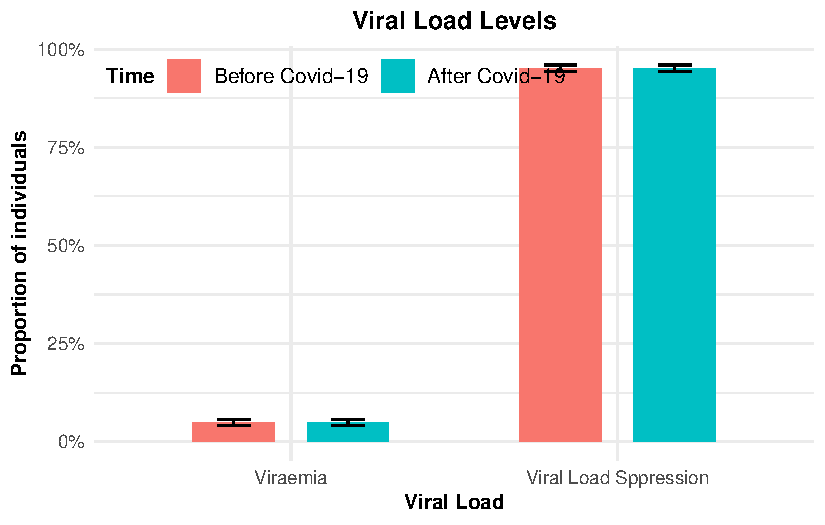
\includegraphics[keepaspectratio]{Rakai_revision_files/figure-pdf/unnamed-chunk-13-1.pdf}}

\subsubsection{\texorpdfstring{\textbf{Proportion taking ART pills less
frequently / in smaller amounts by
Sex}}{Proportion taking ART pills less frequently / in smaller amounts by Sex}}\label{proportion-taking-art-pills-less-frequently-in-smaller-amounts-by-sex}

\begin{Shaded}
\begin{Highlighting}[]
\NormalTok{df6 }\SpecialCharTok{\%\textgreater{}\%} \FunctionTok{group\_by}\NormalTok{(sex,artstrbc) }\SpecialCharTok{\%\textgreater{}\%} 
  \FunctionTok{count}\NormalTok{()}
\end{Highlighting}
\end{Shaded}

\begin{longtable}[]{@{}llr@{}}
\toprule\noalign{}
sex & artstrbc & n \\
\midrule\noalign{}
\endhead
\bottomrule\noalign{}
\endlastfoot
Female & No & 1799 \\
Female & Yes & 21 \\
Male & No & 1003 \\
Male & Yes & 11 \\
\end{longtable}

\begin{Shaded}
\begin{Highlighting}[]
\NormalTok{df6 }\SpecialCharTok{\%\textgreater{}\%} \FunctionTok{group\_by}\NormalTok{(sex,artstrac) }\SpecialCharTok{\%\textgreater{}\%} 
  \FunctionTok{count}\NormalTok{()}
\end{Highlighting}
\end{Shaded}

\begin{longtable}[]{@{}llr@{}}
\toprule\noalign{}
sex & artstrac & n \\
\midrule\noalign{}
\endhead
\bottomrule\noalign{}
\endlastfoot
Female & No & 1775 \\
Female & Yes & 45 \\
Male & No & 985 \\
Male & Yes & 29 \\
\end{longtable}

\begin{Shaded}
\begin{Highlighting}[]
\NormalTok{df\_artstr }\OtherTok{\textless{}{-}}\NormalTok{ df6 }\SpecialCharTok{\%\textgreater{}\%}
  \FunctionTok{pivot\_longer}\NormalTok{(}
    \AttributeTok{cols =} \FunctionTok{c}\NormalTok{(artstrbc, artstrac),}
    \AttributeTok{names\_to =} \StringTok{"variable"}\NormalTok{,}
    \AttributeTok{values\_to =} \StringTok{"response"}
\NormalTok{  ) }\SpecialCharTok{\%\textgreater{}\%}
  \FunctionTok{mutate}\NormalTok{(}
    \AttributeTok{time =} \FunctionTok{if\_else}\NormalTok{(}\FunctionTok{grepl}\NormalTok{(}\StringTok{"bc$"}\NormalTok{, variable), }\StringTok{"Before Covid{-}19"}\NormalTok{, }\StringTok{"After Covid{-}19"}\NormalTok{)}
\NormalTok{  )}

\NormalTok{df\_artstr\_summary }\OtherTok{\textless{}{-}}\NormalTok{ df\_artstr }\SpecialCharTok{\%\textgreater{}\%}
  \FunctionTok{group\_by}\NormalTok{(time,sex) }\SpecialCharTok{\%\textgreater{}\%}
  \FunctionTok{summarise}\NormalTok{(}
    \AttributeTok{n\_yes =} \FunctionTok{sum}\NormalTok{(response }\SpecialCharTok{==} \StringTok{"Yes"}\NormalTok{, }\AttributeTok{na.rm =} \ConstantTok{TRUE}\NormalTok{),}
    \AttributeTok{n =} \FunctionTok{n}\NormalTok{(),}
    \AttributeTok{.groups =} \StringTok{"drop"}
\NormalTok{  )}

\NormalTok{df\_artstr\_totals }\OtherTok{\textless{}{-}}\NormalTok{ df\_artstr }\SpecialCharTok{\%\textgreater{}\%}
  \FunctionTok{group\_by}\NormalTok{(time) }\SpecialCharTok{\%\textgreater{}\%}
  \FunctionTok{summarise}\NormalTok{(}
    \AttributeTok{n\_yes =} \FunctionTok{sum}\NormalTok{(response }\SpecialCharTok{==} \StringTok{"Yes"}\NormalTok{, }\AttributeTok{na.rm =} \ConstantTok{TRUE}\NormalTok{),}
    \AttributeTok{n =} \FunctionTok{n}\NormalTok{(),}
    \AttributeTok{.groups =} \StringTok{"drop"}
\NormalTok{  ) }

\NormalTok{df\_artstr\_summary }\OtherTok{\textless{}{-}} \FunctionTok{bind\_rows}\NormalTok{(df\_artstr\_summary, df\_artstr\_totals) }\SpecialCharTok{\%\textgreater{}\%}
  \FunctionTok{mutate}\NormalTok{(}
    \AttributeTok{proportion =}\NormalTok{ n\_yes }\SpecialCharTok{/}\NormalTok{ n,}
    \AttributeTok{se =} \FunctionTok{sqrt}\NormalTok{(proportion }\SpecialCharTok{*}\NormalTok{ (}\DecValTok{1} \SpecialCharTok{{-}}\NormalTok{ proportion) }\SpecialCharTok{/}\NormalTok{ n),}
    \AttributeTok{lower =}\NormalTok{ proportion }\SpecialCharTok{{-}} \FloatTok{1.96} \SpecialCharTok{*}\NormalTok{ se,}
    \AttributeTok{upper =}\NormalTok{ proportion }\SpecialCharTok{+} \FloatTok{1.96} \SpecialCharTok{*}\NormalTok{ se}
\NormalTok{  ) }\SpecialCharTok{\%\textgreater{}\%} 
  \FunctionTok{mutate}\NormalTok{(}\AttributeTok{time =} \FunctionTok{as\_factor}\NormalTok{(time) }\SpecialCharTok{\%\textgreater{}\%} 
           \FunctionTok{fct\_relevel}\NormalTok{(}\StringTok{"Before Covid{-}19"}\NormalTok{),}
         \AttributeTok{sex=} \FunctionTok{if\_else}\NormalTok{(}\FunctionTok{is.na}\NormalTok{(sex),}\StringTok{"Total"}\NormalTok{,sex))}



\NormalTok{df\_artstr\_summary }\OtherTok{\textless{}{-}}\NormalTok{  df\_artstr\_summary }\SpecialCharTok{\%\textgreater{}\%} 
  \FunctionTok{mutate}\NormalTok{(}
    \AttributeTok{time =} \FunctionTok{as\_factor}\NormalTok{(time) }\SpecialCharTok{\%\textgreater{}\%} 
      \FunctionTok{fct\_relevel}\NormalTok{(}\StringTok{"Before Covid{-}19"}\NormalTok{),}
    \AttributeTok{sex =} \FunctionTok{as\_factor}\NormalTok{(sex)}
\NormalTok{  )}
\end{Highlighting}
\end{Shaded}

\begin{Shaded}
\begin{Highlighting}[]
\NormalTok{reduced\_art\_intake\_plot }\OtherTok{\textless{}{-}} \FunctionTok{ggplot}\NormalTok{(df\_artstr\_summary, }\FunctionTok{aes}\NormalTok{(}\AttributeTok{x =}\NormalTok{ sex, }\AttributeTok{y =}\NormalTok{ proportion, }\AttributeTok{fill =}\NormalTok{ time)) }\SpecialCharTok{+}
  \FunctionTok{geom\_col}\NormalTok{(}\AttributeTok{position =} \FunctionTok{position\_dodge}\NormalTok{(}\AttributeTok{width =} \FloatTok{0.7}\NormalTok{), }\AttributeTok{width =} \FloatTok{0.5}\NormalTok{) }\SpecialCharTok{+}
  \FunctionTok{geom\_errorbar}\NormalTok{(}
    \FunctionTok{aes}\NormalTok{(}\AttributeTok{ymin =}\NormalTok{ lower, }\AttributeTok{ymax =}\NormalTok{ upper),}
    \AttributeTok{position =} \FunctionTok{position\_dodge}\NormalTok{(}\AttributeTok{width =} \FloatTok{0.7}\NormalTok{),}
    \AttributeTok{width =} \FloatTok{0.2}\NormalTok{,}
    \AttributeTok{size =} \DecValTok{1}
\NormalTok{  ) }\SpecialCharTok{+}
  \FunctionTok{scale\_y\_continuous}\NormalTok{(}\AttributeTok{labels =}\NormalTok{ scales}\SpecialCharTok{::}\FunctionTok{percent\_format}\NormalTok{(}\AttributeTok{accuracy =} \DecValTok{1}\NormalTok{),}\AttributeTok{limits =} \FunctionTok{c}\NormalTok{(}\DecValTok{0}\NormalTok{, }\FloatTok{0.20}\NormalTok{))}\SpecialCharTok{+}
  \FunctionTok{labs}\NormalTok{(}
    \AttributeTok{title =} \StringTok{"Reduced ART Intake"}\NormalTok{,}
    \AttributeTok{x =} \StringTok{"Sex"}\NormalTok{,}
    \AttributeTok{y =} \StringTok{"Proportion of Individuals"}\NormalTok{,}
    \AttributeTok{fill =} \StringTok{"Time"}
\NormalTok{  ) }\SpecialCharTok{+}
  \FunctionTok{theme\_minimal}\NormalTok{() }\SpecialCharTok{+}
  \FunctionTok{theme}\NormalTok{(}
    \AttributeTok{plot.title =} \FunctionTok{element\_text}\NormalTok{(}\AttributeTok{hjust =} \FloatTok{0.5}\NormalTok{, }\AttributeTok{face =} \StringTok{"bold"}\NormalTok{, }\AttributeTok{size =} \DecValTok{12}\NormalTok{),}
    \AttributeTok{axis.title.x =} \FunctionTok{element\_text}\NormalTok{(}\AttributeTok{face =} \StringTok{"bold"}\NormalTok{, }\AttributeTok{size =} \DecValTok{10}\NormalTok{),}
    \AttributeTok{axis.title.y =} \FunctionTok{element\_text}\NormalTok{(}\AttributeTok{face =} \StringTok{"bold"}\NormalTok{, }\AttributeTok{size =} \DecValTok{10}\NormalTok{),}
    \AttributeTok{legend.title =} \FunctionTok{element\_text}\NormalTok{(}\AttributeTok{face =} \StringTok{"bold"}\NormalTok{, }\AttributeTok{size =} \DecValTok{10}\NormalTok{),}
    \AttributeTok{legend.text =} \FunctionTok{element\_text}\NormalTok{(}\AttributeTok{size =} \DecValTok{10}\NormalTok{),}
    \AttributeTok{legend.position =} \FunctionTok{c}\NormalTok{(}\DecValTok{0}\NormalTok{, }\DecValTok{1}\NormalTok{),}
    \AttributeTok{legend.justification =} \FunctionTok{c}\NormalTok{(}\DecValTok{0}\NormalTok{, }\DecValTok{1}\NormalTok{),}
    \AttributeTok{legend.direction =} \StringTok{"horizontal"}
\NormalTok{  )}

\NormalTok{reduced\_art\_intake\_plot}
\end{Highlighting}
\end{Shaded}

\pandocbounded{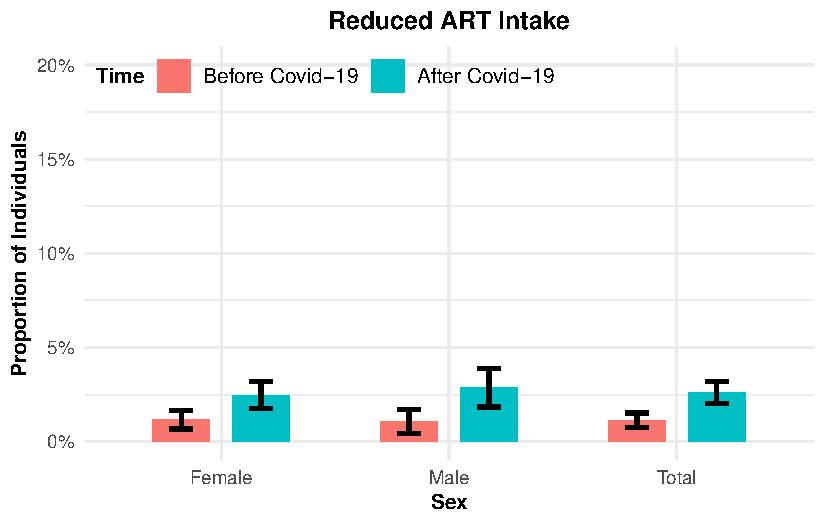
\includegraphics[keepaspectratio]{Rakai_revision_files/figure-pdf/unnamed-chunk-16-1.pdf}}

\subsubsection{\texorpdfstring{\textbf{Run out of ART before next refill
by
Sex}}{Run out of ART before next refill by Sex}}\label{run-out-of-art-before-next-refill-by-sex}

\begin{Shaded}
\begin{Highlighting}[]
\NormalTok{df6 }\SpecialCharTok{\%\textgreater{}\%} \FunctionTok{group\_by}\NormalTok{(sex,artrunbc) }\SpecialCharTok{\%\textgreater{}\%} 
  \FunctionTok{count}\NormalTok{()}
\end{Highlighting}
\end{Shaded}

\begin{longtable}[]{@{}llr@{}}
\toprule\noalign{}
sex & artrunbc & n \\
\midrule\noalign{}
\endhead
\bottomrule\noalign{}
\endlastfoot
Female & No & 1777 \\
Female & Yes & 43 \\
Male & No & 990 \\
Male & Yes & 24 \\
\end{longtable}

\begin{Shaded}
\begin{Highlighting}[]
\NormalTok{df6 }\SpecialCharTok{\%\textgreater{}\%} \FunctionTok{group\_by}\NormalTok{(sex,artrunac) }\SpecialCharTok{\%\textgreater{}\%} 
  \FunctionTok{count}\NormalTok{()}
\end{Highlighting}
\end{Shaded}

\begin{longtable}[]{@{}llr@{}}
\toprule\noalign{}
sex & artrunac & n \\
\midrule\noalign{}
\endhead
\bottomrule\noalign{}
\endlastfoot
Female & No & 1714 \\
Female & Yes & 106 \\
Male & No & 968 \\
Male & Yes & 46 \\
\end{longtable}

\begin{Shaded}
\begin{Highlighting}[]
\NormalTok{df\_artrun }\OtherTok{\textless{}{-}}\NormalTok{ df6 }\SpecialCharTok{\%\textgreater{}\%}
  \FunctionTok{pivot\_longer}\NormalTok{(}
    \AttributeTok{cols =} \FunctionTok{c}\NormalTok{(artrunbc, artrunac),}
    \AttributeTok{names\_to =} \StringTok{"variable"}\NormalTok{,}
    \AttributeTok{values\_to =} \StringTok{"response"}
\NormalTok{  ) }\SpecialCharTok{\%\textgreater{}\%}
  \FunctionTok{mutate}\NormalTok{(}
    \AttributeTok{time =} \FunctionTok{if\_else}\NormalTok{(}\FunctionTok{grepl}\NormalTok{(}\StringTok{"bc$"}\NormalTok{, variable), }\StringTok{"Before Covid{-}19"}\NormalTok{, }\StringTok{"After Covid{-}19"}\NormalTok{),}
    \AttributeTok{variable =} \StringTok{"Run out of ART before next refill"}
\NormalTok{  )}


\NormalTok{df\_artrun\_summary }\OtherTok{\textless{}{-}}\NormalTok{ df\_artrun }\SpecialCharTok{\%\textgreater{}\%}
  \FunctionTok{group\_by}\NormalTok{(time,sex) }\SpecialCharTok{\%\textgreater{}\%}
  \FunctionTok{summarise}\NormalTok{(}
    \AttributeTok{n\_yes =} \FunctionTok{sum}\NormalTok{(response }\SpecialCharTok{==} \StringTok{"Yes"}\NormalTok{, }\AttributeTok{na.rm =} \ConstantTok{TRUE}\NormalTok{),}
    \AttributeTok{n =} \FunctionTok{n}\NormalTok{(),}
    \AttributeTok{.groups =} \StringTok{"drop"}
\NormalTok{  )}

\NormalTok{df\_artrun\_totals }\OtherTok{\textless{}{-}}\NormalTok{ df\_artrun }\SpecialCharTok{\%\textgreater{}\%}
  \FunctionTok{group\_by}\NormalTok{(time) }\SpecialCharTok{\%\textgreater{}\%}
  \FunctionTok{summarise}\NormalTok{(}
    \AttributeTok{n\_yes =} \FunctionTok{sum}\NormalTok{(response }\SpecialCharTok{==} \StringTok{"Yes"}\NormalTok{, }\AttributeTok{na.rm =} \ConstantTok{TRUE}\NormalTok{),}
    \AttributeTok{n =} \FunctionTok{n}\NormalTok{(),}
    \AttributeTok{.groups =} \StringTok{"drop"}
\NormalTok{  )}
 

\NormalTok{df\_artrun\_totals}
\end{Highlighting}
\end{Shaded}

\begin{longtable}[]{@{}lrr@{}}
\toprule\noalign{}
time & n\_yes & n \\
\midrule\noalign{}
\endhead
\bottomrule\noalign{}
\endlastfoot
After Covid-19 & 152 & 2834 \\
Before Covid-19 & 67 & 2834 \\
\end{longtable}

\begin{Shaded}
\begin{Highlighting}[]
\NormalTok{df\_artrun\_summary }\OtherTok{\textless{}{-}} \FunctionTok{bind\_rows}\NormalTok{(df\_artrun\_summary, df\_artrun\_totals) }\SpecialCharTok{\%\textgreater{}\%}
  \FunctionTok{mutate}\NormalTok{(}
    \AttributeTok{proportion =}\NormalTok{ n\_yes }\SpecialCharTok{/}\NormalTok{ n,}
    \AttributeTok{se =} \FunctionTok{sqrt}\NormalTok{(proportion }\SpecialCharTok{*}\NormalTok{ (}\DecValTok{1} \SpecialCharTok{{-}}\NormalTok{ proportion) }\SpecialCharTok{/}\NormalTok{ n),}
    \AttributeTok{lower =}\NormalTok{ proportion }\SpecialCharTok{{-}} \FloatTok{1.96} \SpecialCharTok{*}\NormalTok{ se,}
    \AttributeTok{upper =}\NormalTok{ proportion }\SpecialCharTok{+} \FloatTok{1.96} \SpecialCharTok{*}\NormalTok{ se}
\NormalTok{  )}\SpecialCharTok{\%\textgreater{}\%} 
  \FunctionTok{mutate}\NormalTok{(}\AttributeTok{time =} \FunctionTok{as\_factor}\NormalTok{(time) }\SpecialCharTok{\%\textgreater{}\%} 
           \FunctionTok{fct\_relevel}\NormalTok{(}\StringTok{"Before Covid{-}19"}\NormalTok{),}
        \AttributeTok{sex=} \FunctionTok{if\_else}\NormalTok{(}\FunctionTok{is.na}\NormalTok{(sex),}\StringTok{"Total"}\NormalTok{,sex))}


\NormalTok{df\_artrun\_summary }\OtherTok{\textless{}{-}}\NormalTok{  df\_artrun\_summary }\SpecialCharTok{\%\textgreater{}\%} 
  \FunctionTok{mutate}\NormalTok{(}
    \AttributeTok{time =} \FunctionTok{as\_factor}\NormalTok{(time) }\SpecialCharTok{\%\textgreater{}\%} 
      \FunctionTok{fct\_relevel}\NormalTok{(}\StringTok{"Before Covid{-}19"}\NormalTok{),}
    \AttributeTok{sex =} \FunctionTok{as\_factor}\NormalTok{(sex)}
\NormalTok{  )}
\end{Highlighting}
\end{Shaded}

\begin{Shaded}
\begin{Highlighting}[]
\NormalTok{run\_out\_of\_art\_plot }\OtherTok{\textless{}{-}} \FunctionTok{ggplot}\NormalTok{(df\_artrun\_summary, }\FunctionTok{aes}\NormalTok{(}\AttributeTok{x =}\NormalTok{ sex, }\AttributeTok{y =}\NormalTok{ proportion,}\AttributeTok{fill =}\NormalTok{ time)) }\SpecialCharTok{+}
  \FunctionTok{geom\_col}\NormalTok{(}\AttributeTok{position =} \FunctionTok{position\_dodge}\NormalTok{(}\AttributeTok{width =} \FloatTok{0.7}\NormalTok{), }\AttributeTok{width =} \FloatTok{0.5}\NormalTok{) }\SpecialCharTok{+}
  \FunctionTok{geom\_errorbar}\NormalTok{(}
    \FunctionTok{aes}\NormalTok{(}\AttributeTok{ymin =}\NormalTok{ lower, }\AttributeTok{ymax =}\NormalTok{ upper),}
    \AttributeTok{position =} \FunctionTok{position\_dodge}\NormalTok{(}\AttributeTok{width =} \FloatTok{0.7}\NormalTok{),}
    \AttributeTok{width =} \FloatTok{0.2}\NormalTok{,}
    \AttributeTok{size =} \DecValTok{1}
\NormalTok{  ) }\SpecialCharTok{+}
  \FunctionTok{scale\_y\_continuous}\NormalTok{(}\AttributeTok{labels =}\NormalTok{ scales}\SpecialCharTok{::}\FunctionTok{percent\_format}\NormalTok{(}\AttributeTok{accuracy =} \DecValTok{1}\NormalTok{),}\AttributeTok{limits =} \FunctionTok{c}\NormalTok{(}\DecValTok{0}\NormalTok{, }\FloatTok{0.20}\NormalTok{)) }\SpecialCharTok{+}
  \FunctionTok{labs}\NormalTok{(}
    \AttributeTok{title =} \StringTok{"Run Out of ART"}\NormalTok{,}
    \AttributeTok{x =} \StringTok{"Sex"}\NormalTok{,}
    \AttributeTok{y =} \StringTok{"Proportion of individuals"}\NormalTok{,}
    \AttributeTok{fill =} \StringTok{"Time"}
\NormalTok{  ) }\SpecialCharTok{+}
  \FunctionTok{theme\_minimal}\NormalTok{() }\SpecialCharTok{+}
  \FunctionTok{theme}\NormalTok{(}
    \AttributeTok{plot.title =} \FunctionTok{element\_text}\NormalTok{(}\AttributeTok{hjust =} \FloatTok{0.5}\NormalTok{, }\AttributeTok{face =} \StringTok{"bold"}\NormalTok{, }\AttributeTok{size =} \DecValTok{12}\NormalTok{),}
    \AttributeTok{axis.title.x =} \FunctionTok{element\_text}\NormalTok{(}\AttributeTok{face =} \StringTok{"bold"}\NormalTok{, }\AttributeTok{size =} \DecValTok{10}\NormalTok{),}
    \AttributeTok{axis.title.y =} \FunctionTok{element\_text}\NormalTok{(}\AttributeTok{face =} \StringTok{"bold"}\NormalTok{, }\AttributeTok{size =} \DecValTok{10}\NormalTok{),}
    \AttributeTok{legend.title =} \FunctionTok{element\_text}\NormalTok{(}\AttributeTok{face =} \StringTok{"bold"}\NormalTok{, }\AttributeTok{size =} \DecValTok{10}\NormalTok{),}
    \AttributeTok{legend.text =} \FunctionTok{element\_text}\NormalTok{(}\AttributeTok{size =} \DecValTok{10}\NormalTok{),}
    \AttributeTok{legend.position =} \FunctionTok{c}\NormalTok{(}\DecValTok{0}\NormalTok{, }\DecValTok{1}\NormalTok{),}
    \AttributeTok{legend.justification =} \FunctionTok{c}\NormalTok{(}\DecValTok{0}\NormalTok{, }\DecValTok{1}\NormalTok{),}
    \AttributeTok{legend.direction =} \StringTok{"horizontal"}
\NormalTok{  )}
\NormalTok{run\_out\_of\_art\_plot}
\end{Highlighting}
\end{Shaded}

\pandocbounded{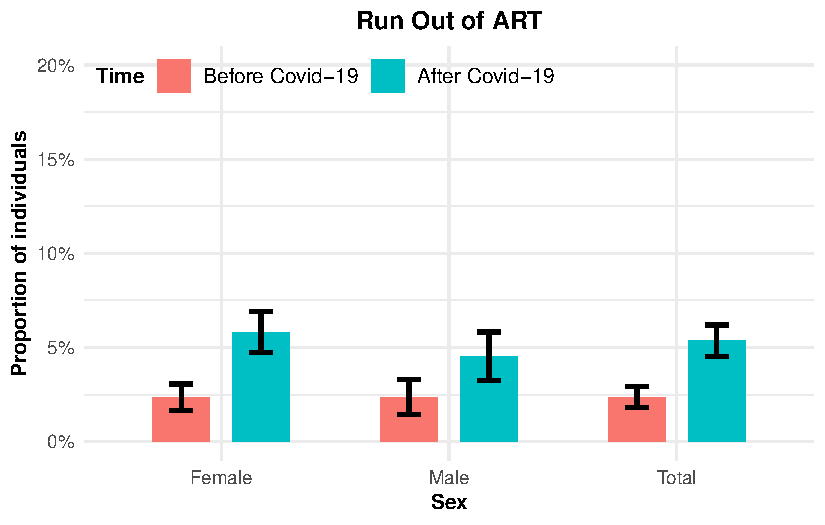
\includegraphics[keepaspectratio]{Rakai_revision_files/figure-pdf/unnamed-chunk-19-1.pdf}}

\subsubsection{\texorpdfstring{\textbf{Missed Scheduled Visits by
Sex}}{Missed Scheduled Visits by Sex}}\label{missed-scheduled-visits-by-sex}

\begin{Shaded}
\begin{Highlighting}[]
\NormalTok{df6 }\SpecialCharTok{\%\textgreater{}\%} \FunctionTok{group\_by}\NormalTok{(sex,hivbc) }\SpecialCharTok{\%\textgreater{}\%} 
  \FunctionTok{count}\NormalTok{()}
\end{Highlighting}
\end{Shaded}

\begin{longtable}[]{@{}llr@{}}
\toprule\noalign{}
sex & hivbc & n \\
\midrule\noalign{}
\endhead
\bottomrule\noalign{}
\endlastfoot
Female & No & 1763 \\
Female & Yes & 57 \\
Male & No & 976 \\
Male & Yes & 38 \\
\end{longtable}

\begin{Shaded}
\begin{Highlighting}[]
\NormalTok{df6 }\SpecialCharTok{\%\textgreater{}\%} \FunctionTok{group\_by}\NormalTok{(sex,hivac) }\SpecialCharTok{\%\textgreater{}\%} 
  \FunctionTok{count}\NormalTok{()}
\end{Highlighting}
\end{Shaded}

\begin{longtable}[]{@{}llr@{}}
\toprule\noalign{}
sex & hivac & n \\
\midrule\noalign{}
\endhead
\bottomrule\noalign{}
\endlastfoot
Female & No & 1642 \\
Female & Yes & 178 \\
Male & No & 917 \\
Male & Yes & 97 \\
\end{longtable}

\begin{Shaded}
\begin{Highlighting}[]
\NormalTok{df\_hiv }\OtherTok{\textless{}{-}}\NormalTok{ df6 }\SpecialCharTok{\%\textgreater{}\%}
  \FunctionTok{pivot\_longer}\NormalTok{(}
    \AttributeTok{cols =} \FunctionTok{c}\NormalTok{(hivbc, hivac),}
    \AttributeTok{names\_to =} \StringTok{"variable"}\NormalTok{,}
    \AttributeTok{values\_to =} \StringTok{"response"}
\NormalTok{  ) }\SpecialCharTok{\%\textgreater{}\%}
  \FunctionTok{mutate}\NormalTok{(}
    \AttributeTok{time =} \FunctionTok{if\_else}\NormalTok{(}\FunctionTok{grepl}\NormalTok{(}\StringTok{"bc$"}\NormalTok{, variable), }\StringTok{"Before Covid{-}19"}\NormalTok{, }\StringTok{"After Covid{-}19"}\NormalTok{),}
    \AttributeTok{variable =} \StringTok{"Missed Scheduled Visits"}
\NormalTok{  )}

\NormalTok{df\_hiv\_summary }\OtherTok{\textless{}{-}}\NormalTok{ df\_hiv }\SpecialCharTok{\%\textgreater{}\%}
  \FunctionTok{group\_by}\NormalTok{(time,sex) }\SpecialCharTok{\%\textgreater{}\%}
  \FunctionTok{summarise}\NormalTok{(}
    \AttributeTok{n\_yes =} \FunctionTok{sum}\NormalTok{(response }\SpecialCharTok{==} \StringTok{"Yes"}\NormalTok{, }\AttributeTok{na.rm =} \ConstantTok{TRUE}\NormalTok{),}
    \AttributeTok{n =} \FunctionTok{n}\NormalTok{(),}
    \AttributeTok{.groups =} \StringTok{"drop"}
\NormalTok{  )}

\NormalTok{df\_hiv\_totals }\OtherTok{\textless{}{-}}\NormalTok{ df\_hiv }\SpecialCharTok{\%\textgreater{}\%}
  \FunctionTok{group\_by}\NormalTok{(time) }\SpecialCharTok{\%\textgreater{}\%}
  \FunctionTok{summarise}\NormalTok{(}
    \AttributeTok{n\_yes =} \FunctionTok{sum}\NormalTok{(response }\SpecialCharTok{==} \StringTok{"Yes"}\NormalTok{, }\AttributeTok{na.rm =} \ConstantTok{TRUE}\NormalTok{),}
    \AttributeTok{n =} \FunctionTok{n}\NormalTok{(),}
    \AttributeTok{.groups =} \StringTok{"drop"}
\NormalTok{  )}

\NormalTok{df\_hiv\_summary }\OtherTok{\textless{}{-}} \FunctionTok{bind\_rows}\NormalTok{(df\_hiv\_summary, df\_hiv\_totals) }\SpecialCharTok{\%\textgreater{}\%}
  \FunctionTok{mutate}\NormalTok{(}
    \AttributeTok{proportion =}\NormalTok{ n\_yes }\SpecialCharTok{/}\NormalTok{ n,}
    \AttributeTok{se =} \FunctionTok{sqrt}\NormalTok{(proportion }\SpecialCharTok{*}\NormalTok{ (}\DecValTok{1} \SpecialCharTok{{-}}\NormalTok{ proportion) }\SpecialCharTok{/}\NormalTok{ n),}
    \AttributeTok{lower =}\NormalTok{ proportion }\SpecialCharTok{{-}} \FloatTok{1.96} \SpecialCharTok{*}\NormalTok{ se,}
    \AttributeTok{upper =}\NormalTok{ proportion }\SpecialCharTok{+} \FloatTok{1.96} \SpecialCharTok{*}\NormalTok{ se}
\NormalTok{  )}\SpecialCharTok{\%\textgreater{}\%} 
  \FunctionTok{mutate}\NormalTok{(}\AttributeTok{time =} \FunctionTok{as\_factor}\NormalTok{(time) }\SpecialCharTok{\%\textgreater{}\%} 
           \FunctionTok{fct\_relevel}\NormalTok{(}\StringTok{"Before Covid{-}19"}\NormalTok{),}
         \AttributeTok{sex=} \FunctionTok{if\_else}\NormalTok{(}\FunctionTok{is.na}\NormalTok{(sex),}\StringTok{"Total"}\NormalTok{,sex))}



\NormalTok{df\_hiv\_summary }\OtherTok{\textless{}{-}}\NormalTok{  df\_hiv\_summary }\SpecialCharTok{\%\textgreater{}\%} 
  \FunctionTok{mutate}\NormalTok{(}
    \AttributeTok{time =} \FunctionTok{as\_factor}\NormalTok{(time) }\SpecialCharTok{\%\textgreater{}\%} 
      \FunctionTok{fct\_relevel}\NormalTok{(}\StringTok{"Before Covid{-}19"}\NormalTok{),}
    \AttributeTok{sex =} \FunctionTok{as\_factor}\NormalTok{(sex)}
\NormalTok{  )}
\end{Highlighting}
\end{Shaded}

\begin{Shaded}
\begin{Highlighting}[]
\NormalTok{missed\_scheduled\_visit\_plot }\OtherTok{\textless{}{-}}  \FunctionTok{ggplot}\NormalTok{(df\_hiv\_summary, }\FunctionTok{aes}\NormalTok{(}\AttributeTok{x =}\NormalTok{ sex, }\AttributeTok{y =}\NormalTok{ proportion, }\AttributeTok{fill =}\NormalTok{ time)) }\SpecialCharTok{+}
  \FunctionTok{geom\_col}\NormalTok{(}\AttributeTok{position =} \FunctionTok{position\_dodge}\NormalTok{(}\AttributeTok{width =} \FloatTok{0.7}\NormalTok{), }\AttributeTok{width =} \FloatTok{0.5}\NormalTok{) }\SpecialCharTok{+}
  \FunctionTok{geom\_errorbar}\NormalTok{(}
    \FunctionTok{aes}\NormalTok{(}\AttributeTok{ymin =}\NormalTok{ lower, }\AttributeTok{ymax =}\NormalTok{ upper),}
    \AttributeTok{position =} \FunctionTok{position\_dodge}\NormalTok{(}\AttributeTok{width =} \FloatTok{0.7}\NormalTok{),}
    \AttributeTok{width =} \FloatTok{0.2}\NormalTok{,}
    \AttributeTok{size =} \DecValTok{1}
\NormalTok{  ) }\SpecialCharTok{+}
  \FunctionTok{scale\_y\_continuous}\NormalTok{(}\AttributeTok{labels =}\NormalTok{ scales}\SpecialCharTok{::}\FunctionTok{percent\_format}\NormalTok{(}\AttributeTok{accuracy =} \DecValTok{1}\NormalTok{),}\AttributeTok{limits =} \FunctionTok{c}\NormalTok{(}\DecValTok{0}\NormalTok{, }\FloatTok{0.20}\NormalTok{)) }\SpecialCharTok{+}
  \FunctionTok{labs}\NormalTok{(}
    \AttributeTok{title =} \StringTok{"Missed Scheduled Visits"}\NormalTok{,}
    \AttributeTok{x =} \StringTok{"Sex"}\NormalTok{,}
    \AttributeTok{y =} \StringTok{"Proportion of individuals"}\NormalTok{,}
    \AttributeTok{fill =} \StringTok{"Time"}
\NormalTok{  ) }\SpecialCharTok{+}
  \FunctionTok{theme\_minimal}\NormalTok{() }\SpecialCharTok{+}
  \FunctionTok{theme}\NormalTok{(}
    \AttributeTok{plot.title =} \FunctionTok{element\_text}\NormalTok{(}\AttributeTok{hjust =} \FloatTok{0.5}\NormalTok{, }\AttributeTok{face =} \StringTok{"bold"}\NormalTok{, }\AttributeTok{size =} \DecValTok{12}\NormalTok{),}
    \AttributeTok{axis.title.x =} \FunctionTok{element\_text}\NormalTok{(}\AttributeTok{face =} \StringTok{"bold"}\NormalTok{, }\AttributeTok{size =} \DecValTok{10}\NormalTok{),}
    \AttributeTok{axis.title.y =} \FunctionTok{element\_text}\NormalTok{(}\AttributeTok{face =} \StringTok{"bold"}\NormalTok{, }\AttributeTok{size =} \DecValTok{10}\NormalTok{),}
    \AttributeTok{legend.title =} \FunctionTok{element\_text}\NormalTok{(}\AttributeTok{face =} \StringTok{"bold"}\NormalTok{, }\AttributeTok{size =} \DecValTok{10}\NormalTok{),}
    \AttributeTok{legend.text =} \FunctionTok{element\_text}\NormalTok{(}\AttributeTok{size =} \DecValTok{10}\NormalTok{),}
    \AttributeTok{legend.position =} \FunctionTok{c}\NormalTok{(}\DecValTok{0}\NormalTok{, }\DecValTok{1}\NormalTok{),}
    \AttributeTok{legend.justification =} \FunctionTok{c}\NormalTok{(}\DecValTok{0}\NormalTok{, }\DecValTok{1}\NormalTok{),}
    \AttributeTok{legend.direction =} \StringTok{"horizontal"}
\NormalTok{  )}

\NormalTok{missed\_scheduled\_visit\_plot}
\end{Highlighting}
\end{Shaded}

\pandocbounded{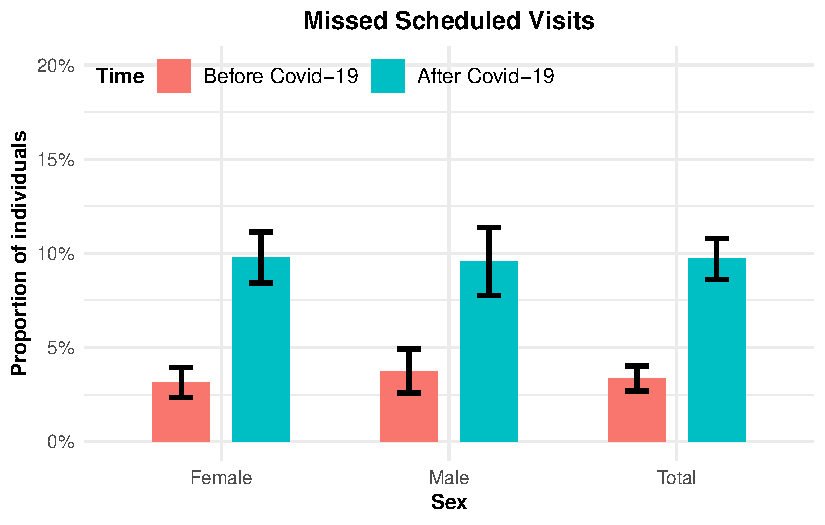
\includegraphics[keepaspectratio]{Rakai_revision_files/figure-pdf/unnamed-chunk-22-1.pdf}}

\subsubsection{Combined Plots}\label{combined-plots}

\begin{Shaded}
\begin{Highlighting}[]
\NormalTok{ps1 }\OtherTok{\textless{}{-}} \FunctionTok{ggplot}\NormalTok{(df\_hiv\_summary, }\FunctionTok{aes}\NormalTok{(}\AttributeTok{x =}\NormalTok{ sex, }\AttributeTok{y =}\NormalTok{ proportion, }\AttributeTok{fill =}\NormalTok{ time)) }\SpecialCharTok{+}
  \FunctionTok{geom\_col}\NormalTok{(}\AttributeTok{position =} \FunctionTok{position\_dodge}\NormalTok{(}\AttributeTok{width =} \FloatTok{0.7}\NormalTok{), }\AttributeTok{width =} \FloatTok{0.5}\NormalTok{) }\SpecialCharTok{+}
  \FunctionTok{geom\_errorbar}\NormalTok{(}
    \FunctionTok{aes}\NormalTok{(}\AttributeTok{ymin =}\NormalTok{ lower, }\AttributeTok{ymax =}\NormalTok{ upper),}
    \AttributeTok{position =} \FunctionTok{position\_dodge}\NormalTok{(}\AttributeTok{width =} \FloatTok{0.7}\NormalTok{),}
    \AttributeTok{width =} \FloatTok{0.2}\NormalTok{,}
    \AttributeTok{size =} \DecValTok{1}
\NormalTok{  ) }\SpecialCharTok{+}
  \FunctionTok{scale\_y\_continuous}\NormalTok{(}\AttributeTok{labels =}\NormalTok{ scales}\SpecialCharTok{::}\FunctionTok{percent\_format}\NormalTok{(}\AttributeTok{accuracy =} \DecValTok{1}\NormalTok{),}\AttributeTok{limits =} \FunctionTok{c}\NormalTok{(}\DecValTok{0}\NormalTok{, }\FloatTok{0.20}\NormalTok{)) }\SpecialCharTok{+}
  \FunctionTok{labs}\NormalTok{(}
    \AttributeTok{title =} \StringTok{"Missed Scheduled Visits"}\NormalTok{,}
    \AttributeTok{x =} \StringTok{"Sex"}\NormalTok{,}
    \AttributeTok{y =} \StringTok{"Proportion of individuals"}\NormalTok{,}
    \AttributeTok{fill =} \StringTok{"Time"}
\NormalTok{  ) }\SpecialCharTok{+}
  \FunctionTok{theme\_minimal}\NormalTok{() }\SpecialCharTok{+}
  \FunctionTok{theme}\NormalTok{(}
    \AttributeTok{plot.title =} \FunctionTok{element\_text}\NormalTok{(}\AttributeTok{hjust =} \FloatTok{0.5}\NormalTok{, }\AttributeTok{face =} \StringTok{"bold"}\NormalTok{, }\AttributeTok{size =} \DecValTok{12}\NormalTok{),}
    \AttributeTok{axis.title.x =} \FunctionTok{element\_text}\NormalTok{(}\AttributeTok{face =} \StringTok{"bold"}\NormalTok{, }\AttributeTok{size =} \DecValTok{10}\NormalTok{),}
    \AttributeTok{axis.title.y =} \FunctionTok{element\_text}\NormalTok{(}\AttributeTok{face =} \StringTok{"bold"}\NormalTok{, }\AttributeTok{size =} \DecValTok{10}\NormalTok{),}
    \AttributeTok{legend.title =} \FunctionTok{element\_text}\NormalTok{(}\AttributeTok{face =} \StringTok{"bold"}\NormalTok{, }\AttributeTok{size =} \DecValTok{10}\NormalTok{),}
    \AttributeTok{legend.text =} \FunctionTok{element\_text}\NormalTok{(}\AttributeTok{size =} \DecValTok{10}\NormalTok{),}
    \AttributeTok{legend.position =} \FunctionTok{c}\NormalTok{(}\DecValTok{0}\NormalTok{, }\DecValTok{1}\NormalTok{),}
    \AttributeTok{legend.justification =} \FunctionTok{c}\NormalTok{(}\DecValTok{0}\NormalTok{, }\DecValTok{1}\NormalTok{),}
    \AttributeTok{legend.direction =} \StringTok{"horizontal"}
\NormalTok{  )}
\NormalTok{ps1 }\DocumentationTok{\#\# Missed scheduled visits}
\end{Highlighting}
\end{Shaded}

\pandocbounded{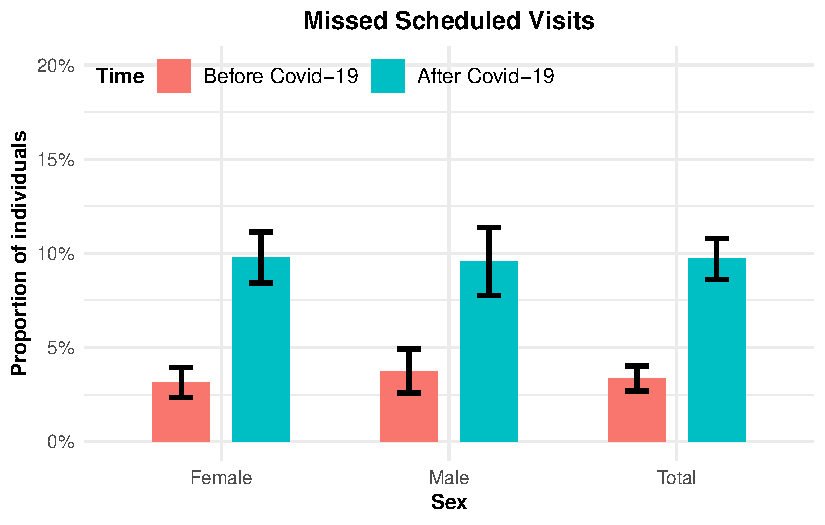
\includegraphics[keepaspectratio]{Rakai_revision_files/figure-pdf/unnamed-chunk-23-1.pdf}}

\begin{Shaded}
\begin{Highlighting}[]
\DocumentationTok{\#\#\# Reduced pill intake}
\NormalTok{ps2 }\OtherTok{\textless{}{-}} \FunctionTok{ggplot}\NormalTok{(df\_artstr\_summary, }\FunctionTok{aes}\NormalTok{(}\AttributeTok{x =}\NormalTok{ sex, }\AttributeTok{y =}\NormalTok{ proportion, }\AttributeTok{fill =}\NormalTok{ time)) }\SpecialCharTok{+}
  \FunctionTok{geom\_col}\NormalTok{(}\AttributeTok{position =} \FunctionTok{position\_dodge}\NormalTok{(}\AttributeTok{width =} \FloatTok{0.7}\NormalTok{), }\AttributeTok{width =} \FloatTok{0.5}\NormalTok{) }\SpecialCharTok{+}
  \FunctionTok{geom\_errorbar}\NormalTok{(}
    \FunctionTok{aes}\NormalTok{(}\AttributeTok{ymin =}\NormalTok{ lower, }\AttributeTok{ymax =}\NormalTok{ upper),}
    \AttributeTok{position =} \FunctionTok{position\_dodge}\NormalTok{(}\AttributeTok{width =} \FloatTok{0.7}\NormalTok{),}
    \AttributeTok{width =} \FloatTok{0.2}\NormalTok{,}
    \AttributeTok{size =} \DecValTok{1}
\NormalTok{  ) }\SpecialCharTok{+}
  \FunctionTok{scale\_y\_continuous}\NormalTok{(}\AttributeTok{labels =}\NormalTok{ scales}\SpecialCharTok{::}\FunctionTok{percent\_format}\NormalTok{(}\AttributeTok{accuracy =} \DecValTok{1}\NormalTok{),}\AttributeTok{limits =} \FunctionTok{c}\NormalTok{(}\DecValTok{0}\NormalTok{, }\FloatTok{0.20}\NormalTok{))}\SpecialCharTok{+}
  \FunctionTok{labs}\NormalTok{(}
    \AttributeTok{title =} \StringTok{" Reduced ART Intake"}\NormalTok{,}
    \AttributeTok{x =} \StringTok{"Sex"}\NormalTok{,}
    \AttributeTok{y =} \StringTok{"Proportion of Individuals"}\NormalTok{,}
    \AttributeTok{fill =} \StringTok{"Time"}
\NormalTok{  ) }\SpecialCharTok{+}
  \FunctionTok{theme\_minimal}\NormalTok{() }\SpecialCharTok{+}
  \FunctionTok{theme}\NormalTok{(}
    \AttributeTok{plot.title =} \FunctionTok{element\_text}\NormalTok{(}\AttributeTok{hjust =} \FloatTok{0.5}\NormalTok{, }\AttributeTok{face =} \StringTok{"bold"}\NormalTok{, }\AttributeTok{size =} \DecValTok{12}\NormalTok{),}
    \AttributeTok{axis.title.x =} \FunctionTok{element\_text}\NormalTok{(}\AttributeTok{face =} \StringTok{"bold"}\NormalTok{, }\AttributeTok{size =} \DecValTok{10}\NormalTok{),}
    \AttributeTok{axis.title.y =} \FunctionTok{element\_text}\NormalTok{(}\AttributeTok{face =} \StringTok{"bold"}\NormalTok{, }\AttributeTok{size =} \DecValTok{10}\NormalTok{),}
    \AttributeTok{legend.title =} \FunctionTok{element\_text}\NormalTok{(}\AttributeTok{face =} \StringTok{"bold"}\NormalTok{, }\AttributeTok{size =} \DecValTok{10}\NormalTok{),}
    \AttributeTok{legend.text =} \FunctionTok{element\_text}\NormalTok{(}\AttributeTok{size =} \DecValTok{10}\NormalTok{),}
    \AttributeTok{legend.position =} \FunctionTok{c}\NormalTok{(}\DecValTok{0}\NormalTok{, }\DecValTok{1}\NormalTok{),}
   \AttributeTok{legend.justification =} \FunctionTok{c}\NormalTok{(}\DecValTok{0}\NormalTok{, }\DecValTok{1}\NormalTok{),}
    \AttributeTok{legend.direction =} \StringTok{"horizontal"}
\NormalTok{  )}
\NormalTok{ps2}
\end{Highlighting}
\end{Shaded}

\pandocbounded{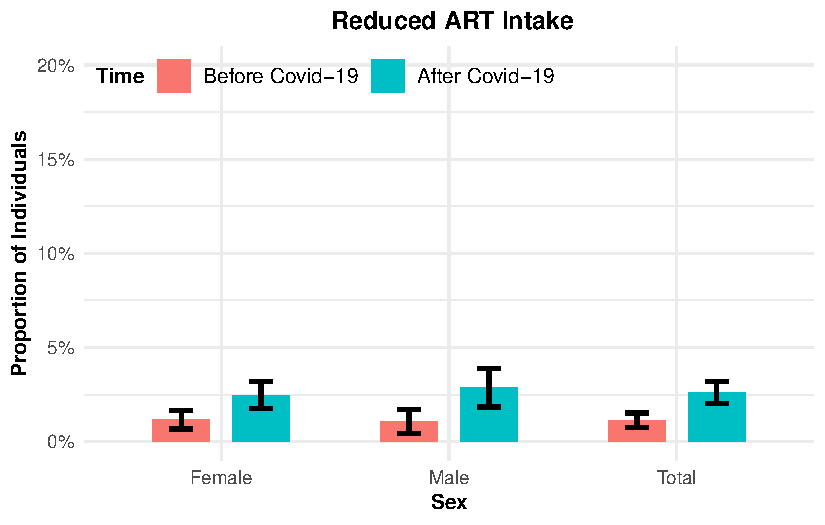
\includegraphics[keepaspectratio]{Rakai_revision_files/figure-pdf/unnamed-chunk-24-1.pdf}}

\begin{Shaded}
\begin{Highlighting}[]
\DocumentationTok{\#\# Run out of pills}
\NormalTok{ps3 }\OtherTok{\textless{}{-}} \FunctionTok{ggplot}\NormalTok{(df\_artrun\_summary, }\FunctionTok{aes}\NormalTok{(}\AttributeTok{x =}\NormalTok{ sex, }\AttributeTok{y =}\NormalTok{ proportion, }\AttributeTok{fill =}\NormalTok{ time)) }\SpecialCharTok{+}
  \FunctionTok{geom\_col}\NormalTok{(}\AttributeTok{position =} \FunctionTok{position\_dodge}\NormalTok{(}\AttributeTok{width =} \FloatTok{0.7}\NormalTok{), }\AttributeTok{width =} \FloatTok{0.5}\NormalTok{) }\SpecialCharTok{+}
  \FunctionTok{geom\_errorbar}\NormalTok{(}
    \FunctionTok{aes}\NormalTok{(}\AttributeTok{ymin =}\NormalTok{ lower, }\AttributeTok{ymax =}\NormalTok{ upper),}
    \AttributeTok{position =} \FunctionTok{position\_dodge}\NormalTok{(}\AttributeTok{width =} \FloatTok{0.7}\NormalTok{),}
    \AttributeTok{width =} \FloatTok{0.2}\NormalTok{,}
    \AttributeTok{size =} \DecValTok{1}
\NormalTok{  ) }\SpecialCharTok{+}
  \FunctionTok{scale\_y\_continuous}\NormalTok{(}\AttributeTok{labels =}\NormalTok{ scales}\SpecialCharTok{::}\FunctionTok{percent\_format}\NormalTok{(}\AttributeTok{accuracy =} \DecValTok{1}\NormalTok{),}\AttributeTok{limits =} \FunctionTok{c}\NormalTok{(}\DecValTok{0}\NormalTok{, }\FloatTok{0.20}\NormalTok{)) }\SpecialCharTok{+}
  \FunctionTok{labs}\NormalTok{(}
    \AttributeTok{title =}  \StringTok{"Run Out of ART"}\NormalTok{,}
    \AttributeTok{x =} \StringTok{"Sex"}\NormalTok{,}
    \AttributeTok{y =} \StringTok{"Proportion of individuals"}\NormalTok{,}
    \AttributeTok{fill =} \StringTok{"Time"}
\NormalTok{  ) }\SpecialCharTok{+}
  \FunctionTok{theme\_minimal}\NormalTok{() }\SpecialCharTok{+}
  \FunctionTok{theme}\NormalTok{(}
    \AttributeTok{plot.title =}  \FunctionTok{element\_text}\NormalTok{(}\AttributeTok{hjust =} \FloatTok{0.5}\NormalTok{, }\AttributeTok{face =} \StringTok{"bold"}\NormalTok{, }\AttributeTok{size =} \DecValTok{12}\NormalTok{),}
    \AttributeTok{axis.title.x =} \FunctionTok{element\_text}\NormalTok{(}\AttributeTok{face =} \StringTok{"bold"}\NormalTok{, }\AttributeTok{size =} \DecValTok{10}\NormalTok{),}
    \AttributeTok{axis.title.y =} \FunctionTok{element\_text}\NormalTok{(}\AttributeTok{face =} \StringTok{"bold"}\NormalTok{, }\AttributeTok{size =} \DecValTok{10}\NormalTok{),}
    \AttributeTok{legend.title =} \FunctionTok{element\_text}\NormalTok{(}\AttributeTok{face =} \StringTok{"bold"}\NormalTok{, }\AttributeTok{size =} \DecValTok{10}\NormalTok{),}
    \AttributeTok{legend.text =} \FunctionTok{element\_text}\NormalTok{(}\AttributeTok{size =} \DecValTok{10}\NormalTok{),}
    \AttributeTok{legend.position =} \FunctionTok{c}\NormalTok{(}\DecValTok{0}\NormalTok{, }\DecValTok{1}\NormalTok{),}
    \AttributeTok{legend.justification =} \FunctionTok{c}\NormalTok{(}\DecValTok{0}\NormalTok{, }\DecValTok{1}\NormalTok{),}
    \AttributeTok{legend.direction =} \StringTok{"horizontal"}
\NormalTok{  )}

\NormalTok{ps3}
\end{Highlighting}
\end{Shaded}

\pandocbounded{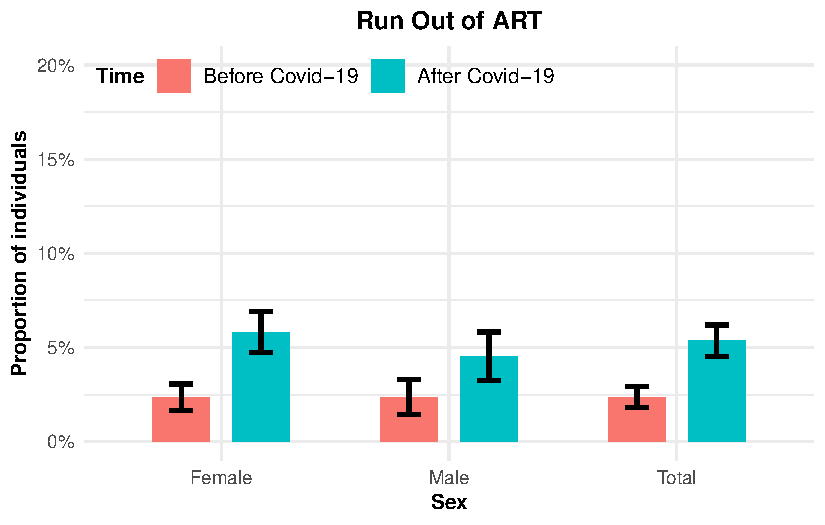
\includegraphics[keepaspectratio]{Rakai_revision_files/figure-pdf/unnamed-chunk-25-1.pdf}}

\begin{Shaded}
\begin{Highlighting}[]
\DocumentationTok{\#\#\# Combined plot}
\NormalTok{(ps1 }\SpecialCharTok{+}\NormalTok{ ps2)}\SpecialCharTok{/}\NormalTok{ps3}
\end{Highlighting}
\end{Shaded}

\pandocbounded{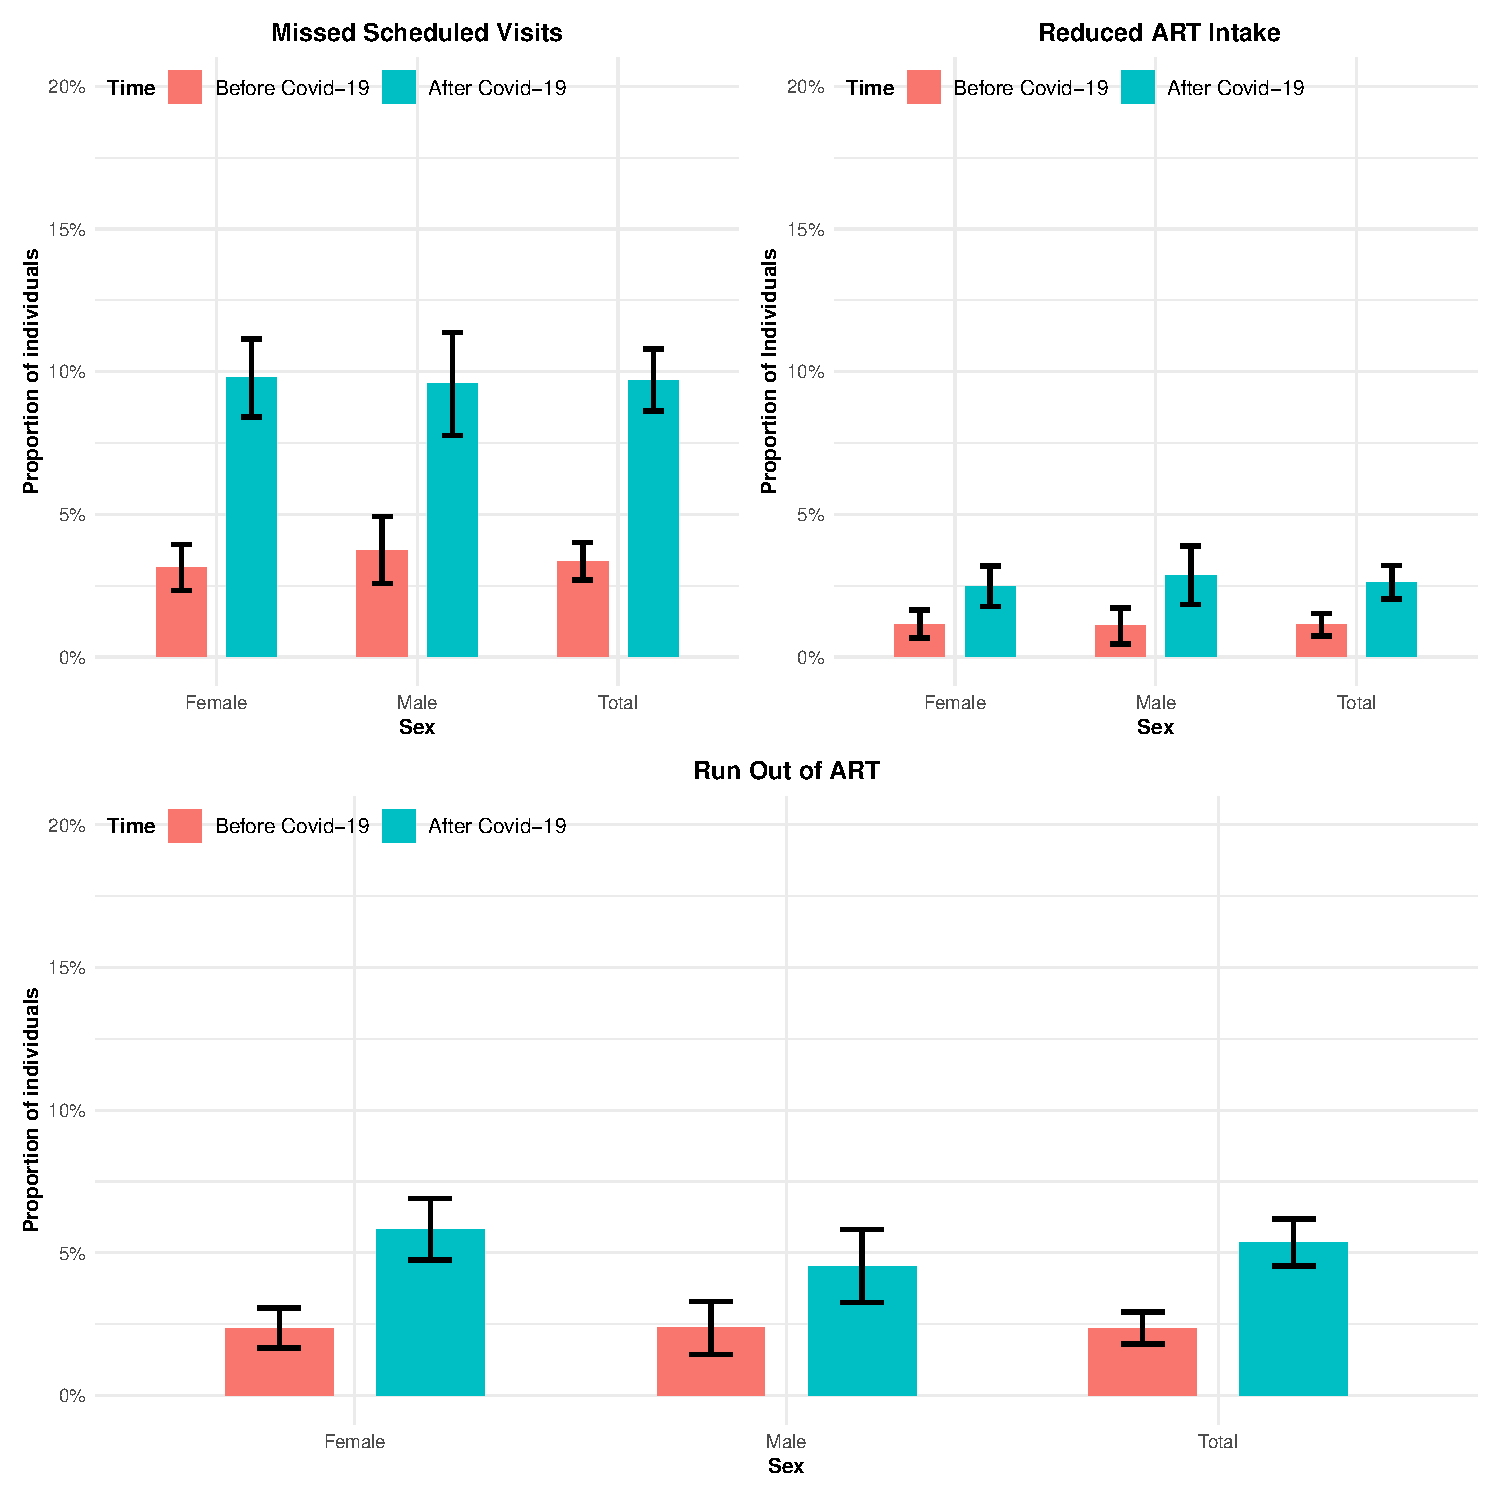
\includegraphics[keepaspectratio]{Rakai_revision_files/figure-pdf/unnamed-chunk-26-1.pdf}}

\section{SUBPLOTS}\label{subplots}

\subsubsection{Community Type}\label{community-type}

\begin{Shaded}
\begin{Highlighting}[]
\NormalTok{df\_com }\OtherTok{\textless{}{-}}\NormalTok{  rakai }\SpecialCharTok{\%\textgreater{}\%} 
  \FunctionTok{select}\NormalTok{(comm\_num,artrunbc,artrunac,}
\NormalTok{         hivac,hivbc,copies,new\_copies,artstrac,artstrbc) }\SpecialCharTok{\%\textgreater{}\%} 
  \FunctionTok{filter}\NormalTok{(hivac }\SpecialCharTok{!=}\DecValTok{8}\NormalTok{, hivbc}\SpecialCharTok{!=}\DecValTok{8}\NormalTok{,artrunbc}\SpecialCharTok{!=}\DecValTok{8}\NormalTok{,artstrac}\SpecialCharTok{!=}\DecValTok{8}\NormalTok{,artstrbc}\SpecialCharTok{!=}\DecValTok{8}\NormalTok{,artrunac}\SpecialCharTok{!=}\DecValTok{8}\NormalTok{) }\SpecialCharTok{\%\textgreater{}\%} 
  \FunctionTok{mutate}\NormalTok{(}
    \AttributeTok{community\_type =} \FunctionTok{case\_when}\NormalTok{(}
\NormalTok{      comm\_num }\SpecialCharTok{\%in\%} \FunctionTok{c}\NormalTok{(}\DecValTok{38}\NormalTok{,}\DecValTok{770}\NormalTok{,}\DecValTok{771}\NormalTok{,}\DecValTok{774}\NormalTok{) }\SpecialCharTok{\textasciitilde{}} \StringTok{"Fishing community"}\NormalTok{,}
      \AttributeTok{.default =} \StringTok{"Inland Community"}\NormalTok{) }\SpecialCharTok{\%\textgreater{}\%} 
      \FunctionTok{fct\_relevel}\NormalTok{(}\StringTok{"Inland Community"}\NormalTok{) }\SpecialCharTok{\%\textgreater{}\%} 
      \FunctionTok{ff\_label}\NormalTok{(}\StringTok{"Community type"}\NormalTok{),}

    \AttributeTok{hivac =} \FunctionTok{if\_else}\NormalTok{(hivac }\SpecialCharTok{==}\DecValTok{1}\NormalTok{, }\StringTok{"Yes"}\NormalTok{,}\StringTok{"No"}\NormalTok{) }\SpecialCharTok{\%\textgreater{}\%} 
    \FunctionTok{ff\_label}\NormalTok{(}\StringTok{"Missed scheduled visit for HIV care"}\NormalTok{) }\SpecialCharTok{\%\textgreater{}\%} 
      \FunctionTok{as\_factor}\NormalTok{(),}
   
     \AttributeTok{hivbc =} \FunctionTok{if\_else}\NormalTok{(hivbc }\SpecialCharTok{==}\DecValTok{1}\NormalTok{,}\StringTok{"Yes"}\NormalTok{,}\StringTok{"No"}\NormalTok{) }\SpecialCharTok{\%\textgreater{}\%} 
    \FunctionTok{ff\_label}\NormalTok{(}\StringTok{"Missed scheduled visit for HIV care"}\NormalTok{) }\SpecialCharTok{\%\textgreater{}\%} 
    \FunctionTok{as\_factor}\NormalTok{(),}
 
     \AttributeTok{artrunac =} \FunctionTok{if\_else}\NormalTok{(artrunac }\SpecialCharTok{==}\DecValTok{1}\NormalTok{,}\StringTok{"Yes"}\NormalTok{,}\StringTok{"No"}\NormalTok{) }\SpecialCharTok{\%\textgreater{}\%} 
    \FunctionTok{as\_factor}\NormalTok{() }\SpecialCharTok{\%\textgreater{}\%} 
    \FunctionTok{ff\_label}\NormalTok{(}\StringTok{"Run out of ART before next refill"}\NormalTok{),}
 
   \AttributeTok{artrunbc =} \FunctionTok{if\_else}\NormalTok{(artrunbc }\SpecialCharTok{==}\DecValTok{1}\NormalTok{,}\StringTok{"Yes"}\NormalTok{,}\StringTok{"No"}\NormalTok{) }\SpecialCharTok{\%\textgreater{}\%} 
    \FunctionTok{as\_factor}\NormalTok{() }\SpecialCharTok{\%\textgreater{}\%} 
    \FunctionTok{ff\_label}\NormalTok{(}\StringTok{"Run out of ART before next refill"}\NormalTok{),}
  
  \AttributeTok{artstrac =} \FunctionTok{if\_else}\NormalTok{(artstrac }\SpecialCharTok{==}\DecValTok{1}\NormalTok{,}\StringTok{"Yes"}\NormalTok{,}\StringTok{"No"}\NormalTok{) }\SpecialCharTok{\%\textgreater{}\%} 
    \FunctionTok{as\_factor}\NormalTok{() }\SpecialCharTok{\%\textgreater{}\%} 
    \FunctionTok{ff\_label}\NormalTok{(}\StringTok{"Taken ART pills less frequently / in smaller}
\StringTok{amounts to conserve supply"}\NormalTok{),}
  
  \AttributeTok{artstrbc =} \FunctionTok{if\_else}\NormalTok{(artstrbc }\SpecialCharTok{==}\DecValTok{1}\NormalTok{,}\StringTok{"Yes"}\NormalTok{,}\StringTok{"No"}\NormalTok{) }\SpecialCharTok{\%\textgreater{}\%} 
    \FunctionTok{as\_factor}\NormalTok{() }\SpecialCharTok{\%\textgreater{}\%} 
    \FunctionTok{ff\_label}\NormalTok{(}\StringTok{"Taken ART pills less frequently / in smaller}
\StringTok{amounts to conserve supply"}\NormalTok{)}
\NormalTok{  ) }\SpecialCharTok{\%\textgreater{}\%} 
  \FunctionTok{select}\NormalTok{(}\SpecialCharTok{{-}}\NormalTok{comm\_num)}
\end{Highlighting}
\end{Shaded}

\begin{Shaded}
\begin{Highlighting}[]
\CommentTok{\# df\_com}
\end{Highlighting}
\end{Shaded}

\subsubsection{Reduced ART intake by
Community}\label{reduced-art-intake-by-community}

\begin{Shaded}
\begin{Highlighting}[]
\NormalTok{df\_com }\SpecialCharTok{\%\textgreater{}\%} \FunctionTok{group\_by}\NormalTok{(community\_type,artstrbc) }\SpecialCharTok{\%\textgreater{}\%} 
  \FunctionTok{count}\NormalTok{()}
\end{Highlighting}
\end{Shaded}

\begin{longtable}[]{@{}llr@{}}
\toprule\noalign{}
community\_type & artstrbc & n \\
\midrule\noalign{}
\endhead
\bottomrule\noalign{}
\endlastfoot
Inland Community & No & 1272 \\
Inland Community & Yes & 11 \\
Fishing community & No & 1530 \\
Fishing community & Yes & 21 \\
\end{longtable}

\begin{Shaded}
\begin{Highlighting}[]
\NormalTok{df\_com }\SpecialCharTok{\%\textgreater{}\%} \FunctionTok{group\_by}\NormalTok{(community\_type,artstrac) }\SpecialCharTok{\%\textgreater{}\%} 
  \FunctionTok{count}\NormalTok{()}
\end{Highlighting}
\end{Shaded}

\begin{longtable}[]{@{}llr@{}}
\toprule\noalign{}
community\_type & artstrac & n \\
\midrule\noalign{}
\endhead
\bottomrule\noalign{}
\endlastfoot
Inland Community & No & 1268 \\
Inland Community & Yes & 15 \\
Fishing community & No & 1492 \\
Fishing community & Yes & 59 \\
\end{longtable}

\begin{Shaded}
\begin{Highlighting}[]
\NormalTok{df\_com\_artstr }\OtherTok{\textless{}{-}}\NormalTok{ df\_com }\SpecialCharTok{\%\textgreater{}\%}
  \FunctionTok{pivot\_longer}\NormalTok{(}
    \AttributeTok{cols =} \FunctionTok{c}\NormalTok{(artstrbc, artstrac),}
    \AttributeTok{names\_to =} \StringTok{"variable"}\NormalTok{,}
    \AttributeTok{values\_to =} \StringTok{"response"}
\NormalTok{  ) }\SpecialCharTok{\%\textgreater{}\%}
  \FunctionTok{mutate}\NormalTok{(}
    \AttributeTok{time =} \FunctionTok{if\_else}\NormalTok{(}\FunctionTok{grepl}\NormalTok{(}\StringTok{"bc$"}\NormalTok{, variable), }\StringTok{"Before Covid{-}19"}\NormalTok{, }\StringTok{"After Covid{-}19"}\NormalTok{)}
\NormalTok{  )}

\NormalTok{df\_com\_artstr\_summary }\OtherTok{\textless{}{-}}\NormalTok{ df\_com\_artstr }\SpecialCharTok{\%\textgreater{}\%}
  \FunctionTok{group\_by}\NormalTok{(time,community\_type) }\SpecialCharTok{\%\textgreater{}\%}
  \FunctionTok{summarise}\NormalTok{(}
    \AttributeTok{n\_yes =} \FunctionTok{sum}\NormalTok{(response }\SpecialCharTok{==} \StringTok{"Yes"}\NormalTok{, }\AttributeTok{na.rm =} \ConstantTok{TRUE}\NormalTok{),}
    \AttributeTok{n =} \FunctionTok{n}\NormalTok{(),}
    \AttributeTok{.groups =} \StringTok{"drop"}
\NormalTok{  )}

\NormalTok{df\_com\_artstr\_totals }\OtherTok{\textless{}{-}}\NormalTok{ df\_com\_artstr }\SpecialCharTok{\%\textgreater{}\%}
  \FunctionTok{group\_by}\NormalTok{(time) }\SpecialCharTok{\%\textgreater{}\%}
  \FunctionTok{summarise}\NormalTok{(}
    \AttributeTok{n\_yes =} \FunctionTok{sum}\NormalTok{(response }\SpecialCharTok{==} \StringTok{"Yes"}\NormalTok{, }\AttributeTok{na.rm =} \ConstantTok{TRUE}\NormalTok{),}
    \AttributeTok{n =} \FunctionTok{n}\NormalTok{(),}
    \AttributeTok{.groups =} \StringTok{"drop"}
\NormalTok{  ) }

\NormalTok{df\_com\_artstr\_summary }\OtherTok{\textless{}{-}} \FunctionTok{bind\_rows}\NormalTok{(df\_com\_artstr\_summary, df\_com\_artstr\_totals) }\SpecialCharTok{\%\textgreater{}\%}
  \FunctionTok{mutate}\NormalTok{(}
    \AttributeTok{proportion =}\NormalTok{ n\_yes }\SpecialCharTok{/}\NormalTok{ n,}
    \AttributeTok{se =} \FunctionTok{sqrt}\NormalTok{(proportion }\SpecialCharTok{*}\NormalTok{ (}\DecValTok{1} \SpecialCharTok{{-}}\NormalTok{ proportion) }\SpecialCharTok{/}\NormalTok{ n),}
    \AttributeTok{lower =}\NormalTok{ proportion }\SpecialCharTok{{-}} \FloatTok{1.96} \SpecialCharTok{*}\NormalTok{ se,}
    \AttributeTok{upper =}\NormalTok{ proportion }\SpecialCharTok{+} \FloatTok{1.96} \SpecialCharTok{*}\NormalTok{ se}
\NormalTok{  ) }\SpecialCharTok{\%\textgreater{}\%} 
  \FunctionTok{mutate}\NormalTok{(}\AttributeTok{time =} \FunctionTok{as\_factor}\NormalTok{(time) }\SpecialCharTok{\%\textgreater{}\%} 
           \FunctionTok{fct\_relevel}\NormalTok{(}\StringTok{"Before Covid{-}19"}\NormalTok{),}
         \AttributeTok{community\_type =} \FunctionTok{if\_else}\NormalTok{(}\FunctionTok{is.na}\NormalTok{(community\_type),}\StringTok{"Total"}\NormalTok{,community\_type))}

\NormalTok{df\_com\_artstr\_summary}
\end{Highlighting}
\end{Shaded}

\begin{longtable}[]{@{}
  >{\raggedright\arraybackslash}p{(\linewidth - 14\tabcolsep) * \real{0.1860}}
  >{\raggedright\arraybackslash}p{(\linewidth - 14\tabcolsep) * \real{0.2093}}
  >{\raggedleft\arraybackslash}p{(\linewidth - 14\tabcolsep) * \real{0.0698}}
  >{\raggedleft\arraybackslash}p{(\linewidth - 14\tabcolsep) * \real{0.0581}}
  >{\raggedleft\arraybackslash}p{(\linewidth - 14\tabcolsep) * \real{0.1279}}
  >{\raggedleft\arraybackslash}p{(\linewidth - 14\tabcolsep) * \real{0.1163}}
  >{\raggedleft\arraybackslash}p{(\linewidth - 14\tabcolsep) * \real{0.1163}}
  >{\raggedleft\arraybackslash}p{(\linewidth - 14\tabcolsep) * \real{0.1163}}@{}}
\toprule\noalign{}
\begin{minipage}[b]{\linewidth}\raggedright
time
\end{minipage} & \begin{minipage}[b]{\linewidth}\raggedright
community\_type
\end{minipage} & \begin{minipage}[b]{\linewidth}\raggedleft
n\_yes
\end{minipage} & \begin{minipage}[b]{\linewidth}\raggedleft
n
\end{minipage} & \begin{minipage}[b]{\linewidth}\raggedleft
proportion
\end{minipage} & \begin{minipage}[b]{\linewidth}\raggedleft
se
\end{minipage} & \begin{minipage}[b]{\linewidth}\raggedleft
lower
\end{minipage} & \begin{minipage}[b]{\linewidth}\raggedleft
upper
\end{minipage} \\
\midrule\noalign{}
\endhead
\bottomrule\noalign{}
\endlastfoot
After Covid-19 & Inland Community & 15 & 1283 & 0.0116913 & 0.0030010 &
0.0058094 & 0.0175733 \\
After Covid-19 & Fishing community & 59 & 1551 & 0.0380400 & 0.0048573 &
0.0285197 & 0.0475602 \\
Before Covid-19 & Inland Community & 11 & 1283 & 0.0085737 & 0.0025739 &
0.0035287 & 0.0136186 \\
Before Covid-19 & Fishing community & 21 & 1551 & 0.0135397 & 0.0029345
& 0.0077880 & 0.0192913 \\
After Covid-19 & Total & 74 & 2834 & 0.0261115 & 0.0029955 & 0.0202403 &
0.0319827 \\
Before Covid-19 & Total & 32 & 2834 & 0.0112915 & 0.0019848 & 0.0074013
& 0.0151816 \\
\end{longtable}

\begin{Shaded}
\begin{Highlighting}[]
\NormalTok{reduced\_art\_intake\_by\_community\_plot }\OtherTok{\textless{}{-}} \FunctionTok{ggplot}\NormalTok{(df\_com\_artstr\_summary, }\FunctionTok{aes}\NormalTok{(}\AttributeTok{x =}\NormalTok{ community\_type, }\AttributeTok{y =}\NormalTok{ proportion, }\AttributeTok{fill =}\NormalTok{ time)) }\SpecialCharTok{+}
  \FunctionTok{geom\_col}\NormalTok{(}\AttributeTok{position =} \FunctionTok{position\_dodge}\NormalTok{(}\AttributeTok{width =} \FloatTok{0.7}\NormalTok{), }\AttributeTok{width =} \FloatTok{0.5}\NormalTok{) }\SpecialCharTok{+}
  \FunctionTok{geom\_errorbar}\NormalTok{(}
    \FunctionTok{aes}\NormalTok{(}\AttributeTok{ymin =}\NormalTok{ lower, }\AttributeTok{ymax =}\NormalTok{ upper),}
    \AttributeTok{position =} \FunctionTok{position\_dodge}\NormalTok{(}\AttributeTok{width =} \FloatTok{0.7}\NormalTok{),}
    \AttributeTok{width =} \FloatTok{0.2}\NormalTok{,}
    \AttributeTok{size =} \DecValTok{1}
\NormalTok{  ) }\SpecialCharTok{+}
  \FunctionTok{scale\_y\_continuous}\NormalTok{(}\AttributeTok{labels =}\NormalTok{ scales}\SpecialCharTok{::}\FunctionTok{percent\_format}\NormalTok{(}\AttributeTok{accuracy =} \DecValTok{1}\NormalTok{),}\AttributeTok{limits =} \FunctionTok{c}\NormalTok{(}\DecValTok{0}\NormalTok{, }\FloatTok{0.12}\NormalTok{))}\SpecialCharTok{+}
  \FunctionTok{labs}\NormalTok{(}
    \AttributeTok{title =} \StringTok{" Reduced ART Intake"}\NormalTok{,}
    \AttributeTok{x =} \StringTok{"Community Type"}\NormalTok{,}
    \AttributeTok{y =} \StringTok{"Proportion of Individuals"}\NormalTok{,}
    \AttributeTok{fill =}  \StringTok{"Time"}
\NormalTok{  ) }\SpecialCharTok{+}
  \FunctionTok{theme\_minimal}\NormalTok{() }\SpecialCharTok{+}
  \FunctionTok{theme}\NormalTok{(}
    \AttributeTok{plot.title =} \FunctionTok{element\_text}\NormalTok{(}\AttributeTok{hjust =} \FloatTok{0.5}\NormalTok{, }\AttributeTok{face =} \StringTok{"bold"}\NormalTok{, }\AttributeTok{size =} \DecValTok{12}\NormalTok{),}
    \AttributeTok{axis.title.x =} \FunctionTok{element\_text}\NormalTok{(}\AttributeTok{face =} \StringTok{"bold"}\NormalTok{, }\AttributeTok{size =} \DecValTok{10}\NormalTok{),}
    \AttributeTok{axis.title.y =} \FunctionTok{element\_text}\NormalTok{(}\AttributeTok{face =} \StringTok{"bold"}\NormalTok{, }\AttributeTok{size =} \DecValTok{10}\NormalTok{),}
    \AttributeTok{legend.title =} \FunctionTok{element\_text}\NormalTok{(}\AttributeTok{face =} \StringTok{"bold"}\NormalTok{, }\AttributeTok{size =} \DecValTok{10}\NormalTok{),}
    \AttributeTok{legend.text =} \FunctionTok{element\_text}\NormalTok{(}\AttributeTok{size =} \DecValTok{10}\NormalTok{),}
    \AttributeTok{legend.position =} \FunctionTok{c}\NormalTok{(}\DecValTok{0}\NormalTok{, }\DecValTok{1}\NormalTok{),}
    \AttributeTok{legend.justification =} \FunctionTok{c}\NormalTok{(}\DecValTok{0}\NormalTok{, }\DecValTok{1}\NormalTok{),}
    \AttributeTok{legend.direction =} \StringTok{"horizontal"}
\NormalTok{  )}

\NormalTok{reduced\_art\_intake\_by\_community\_plot}
\end{Highlighting}
\end{Shaded}

\pandocbounded{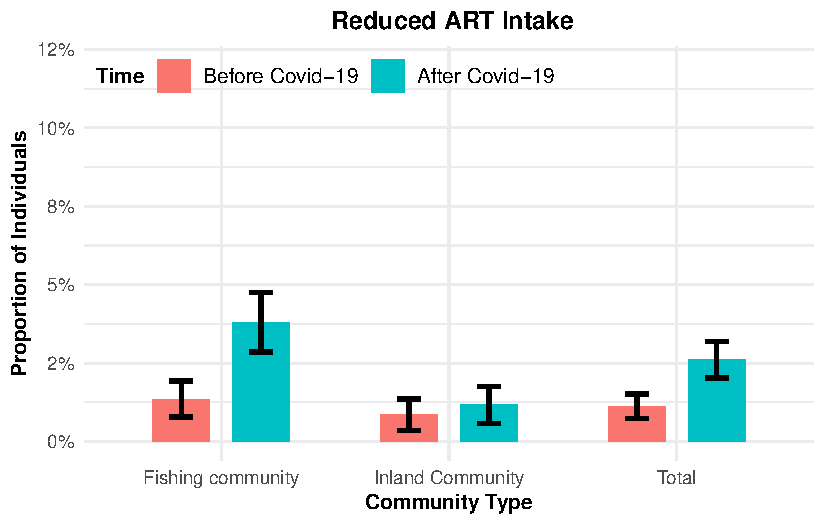
\includegraphics[keepaspectratio]{Rakai_revision_files/figure-pdf/unnamed-chunk-31-1.pdf}}

\subsubsection{Missed Scheduled Visits by
Community}\label{missed-scheduled-visits-by-community}

\begin{Shaded}
\begin{Highlighting}[]
\NormalTok{df\_com }\SpecialCharTok{\%\textgreater{}\%} \FunctionTok{group\_by}\NormalTok{(community\_type,hivbc) }\SpecialCharTok{\%\textgreater{}\%} 
  \FunctionTok{count}\NormalTok{()}
\end{Highlighting}
\end{Shaded}

\begin{longtable}[]{@{}llr@{}}
\toprule\noalign{}
community\_type & hivbc & n \\
\midrule\noalign{}
\endhead
\bottomrule\noalign{}
\endlastfoot
Inland Community & No & 1257 \\
Inland Community & Yes & 26 \\
Fishing community & No & 1482 \\
Fishing community & Yes & 69 \\
\end{longtable}

\begin{Shaded}
\begin{Highlighting}[]
\NormalTok{df\_com }\SpecialCharTok{\%\textgreater{}\%} \FunctionTok{group\_by}\NormalTok{(community\_type,hivac) }\SpecialCharTok{\%\textgreater{}\%} 
  \FunctionTok{count}\NormalTok{()}
\end{Highlighting}
\end{Shaded}

\begin{longtable}[]{@{}llr@{}}
\toprule\noalign{}
community\_type & hivac & n \\
\midrule\noalign{}
\endhead
\bottomrule\noalign{}
\endlastfoot
Inland Community & No & 1198 \\
Inland Community & Yes & 85 \\
Fishing community & No & 1361 \\
Fishing community & Yes & 190 \\
\end{longtable}

\begin{Shaded}
\begin{Highlighting}[]
\NormalTok{df\_com\_hiv }\OtherTok{\textless{}{-}}\NormalTok{ df\_com }\SpecialCharTok{\%\textgreater{}\%}
  \FunctionTok{mutate}\NormalTok{(}
    \AttributeTok{hivbc =} \FunctionTok{as.character}\NormalTok{(hivbc),}
    \AttributeTok{hivac =} \FunctionTok{as.character}\NormalTok{(hivac)}
\NormalTok{  ) }\SpecialCharTok{\%\textgreater{}\%}
  \FunctionTok{pivot\_longer}\NormalTok{(}
    \AttributeTok{cols =} \FunctionTok{c}\NormalTok{(hivbc, hivac),}
    \AttributeTok{names\_to =} \StringTok{"variable"}\NormalTok{,}
    \AttributeTok{values\_to =} \StringTok{"response"}
\NormalTok{  ) }\SpecialCharTok{\%\textgreater{}\%}
  \FunctionTok{mutate}\NormalTok{(}
    \AttributeTok{time =} \FunctionTok{if\_else}\NormalTok{(}\FunctionTok{grepl}\NormalTok{(}\StringTok{"bc$"}\NormalTok{, variable), }\StringTok{"Before Covid{-}19"}\NormalTok{, }\StringTok{"After Covid{-}19"}\NormalTok{)}
\NormalTok{  )}

\NormalTok{df\_com\_hiv\_summary }\OtherTok{\textless{}{-}}\NormalTok{ df\_com\_hiv }\SpecialCharTok{\%\textgreater{}\%}
  \FunctionTok{group\_by}\NormalTok{(time,community\_type) }\SpecialCharTok{\%\textgreater{}\%}
  \FunctionTok{summarise}\NormalTok{(}
    \AttributeTok{n\_yes =} \FunctionTok{sum}\NormalTok{(response }\SpecialCharTok{==} \StringTok{"Yes"}\NormalTok{, }\AttributeTok{na.rm =} \ConstantTok{TRUE}\NormalTok{),}
    \AttributeTok{n =} \FunctionTok{n}\NormalTok{(),}
    \AttributeTok{.groups =} \StringTok{"drop"}
\NormalTok{  )}

\NormalTok{df\_com\_hiv\_totals }\OtherTok{\textless{}{-}}\NormalTok{ df\_com\_hiv }\SpecialCharTok{\%\textgreater{}\%}
  \FunctionTok{group\_by}\NormalTok{(time) }\SpecialCharTok{\%\textgreater{}\%}
  \FunctionTok{summarise}\NormalTok{(}
    \AttributeTok{n\_yes =} \FunctionTok{sum}\NormalTok{(response }\SpecialCharTok{==} \StringTok{"Yes"}\NormalTok{, }\AttributeTok{na.rm =} \ConstantTok{TRUE}\NormalTok{),}
    \AttributeTok{n =} \FunctionTok{n}\NormalTok{(),}
    \AttributeTok{.groups =} \StringTok{"drop"}
\NormalTok{  ) }

\NormalTok{df\_com\_hiv\_summary }\OtherTok{\textless{}{-}} \FunctionTok{bind\_rows}\NormalTok{(df\_com\_hiv\_summary, df\_com\_hiv\_totals) }\SpecialCharTok{\%\textgreater{}\%}
  \FunctionTok{mutate}\NormalTok{(}
    \AttributeTok{proportion =}\NormalTok{ n\_yes }\SpecialCharTok{/}\NormalTok{ n,}
    \AttributeTok{se =} \FunctionTok{sqrt}\NormalTok{(proportion }\SpecialCharTok{*}\NormalTok{ (}\DecValTok{1} \SpecialCharTok{{-}}\NormalTok{ proportion) }\SpecialCharTok{/}\NormalTok{ n),}
    \AttributeTok{lower =}\NormalTok{ proportion }\SpecialCharTok{{-}} \FloatTok{1.96} \SpecialCharTok{*}\NormalTok{ se,}
    \AttributeTok{upper =}\NormalTok{ proportion }\SpecialCharTok{+} \FloatTok{1.96} \SpecialCharTok{*}\NormalTok{ se}
\NormalTok{  )}\SpecialCharTok{\%\textgreater{}\%} 
  \FunctionTok{mutate}\NormalTok{(}\AttributeTok{time =} \FunctionTok{as\_factor}\NormalTok{(time) }\SpecialCharTok{\%\textgreater{}\%} 
           \FunctionTok{fct\_relevel}\NormalTok{(}\StringTok{"Before Covid{-}19"}\NormalTok{),}
         \AttributeTok{community\_type =} \FunctionTok{if\_else}\NormalTok{(}\FunctionTok{is.na}\NormalTok{(community\_type),}\StringTok{"Total"}\NormalTok{,community\_type))}



\NormalTok{df\_com\_hiv\_summary}
\end{Highlighting}
\end{Shaded}

\begin{longtable}[]{@{}
  >{\raggedright\arraybackslash}p{(\linewidth - 14\tabcolsep) * \real{0.1860}}
  >{\raggedright\arraybackslash}p{(\linewidth - 14\tabcolsep) * \real{0.2093}}
  >{\raggedleft\arraybackslash}p{(\linewidth - 14\tabcolsep) * \real{0.0698}}
  >{\raggedleft\arraybackslash}p{(\linewidth - 14\tabcolsep) * \real{0.0581}}
  >{\raggedleft\arraybackslash}p{(\linewidth - 14\tabcolsep) * \real{0.1279}}
  >{\raggedleft\arraybackslash}p{(\linewidth - 14\tabcolsep) * \real{0.1163}}
  >{\raggedleft\arraybackslash}p{(\linewidth - 14\tabcolsep) * \real{0.1163}}
  >{\raggedleft\arraybackslash}p{(\linewidth - 14\tabcolsep) * \real{0.1163}}@{}}
\toprule\noalign{}
\begin{minipage}[b]{\linewidth}\raggedright
time
\end{minipage} & \begin{minipage}[b]{\linewidth}\raggedright
community\_type
\end{minipage} & \begin{minipage}[b]{\linewidth}\raggedleft
n\_yes
\end{minipage} & \begin{minipage}[b]{\linewidth}\raggedleft
n
\end{minipage} & \begin{minipage}[b]{\linewidth}\raggedleft
proportion
\end{minipage} & \begin{minipage}[b]{\linewidth}\raggedleft
se
\end{minipage} & \begin{minipage}[b]{\linewidth}\raggedleft
lower
\end{minipage} & \begin{minipage}[b]{\linewidth}\raggedleft
upper
\end{minipage} \\
\midrule\noalign{}
\endhead
\bottomrule\noalign{}
\endlastfoot
After Covid-19 & Inland Community & 85 & 1283 & 0.0662510 & 0.0069438 &
0.0526411 & 0.0798608 \\
After Covid-19 & Fishing community & 190 & 1551 & 0.1225016 & 0.0083251
& 0.1061845 & 0.1388188 \\
Before Covid-19 & Inland Community & 26 & 1283 & 0.0202650 & 0.0039338 &
0.0125547 & 0.0279753 \\
Before Covid-19 & Fishing community & 69 & 1551 & 0.0444874 & 0.0052352
& 0.0342265 & 0.0547484 \\
After Covid-19 & Total & 275 & 2834 & 0.0970360 & 0.0055603 & 0.0861377
& 0.1079343 \\
Before Covid-19 & Total & 95 & 2834 & 0.0335215 & 0.0033811 & 0.0268946
& 0.0401485 \\
\end{longtable}

\begin{Shaded}
\begin{Highlighting}[]
\NormalTok{missed\_scheduled\_visit\_by\_community\_type\_plot }\OtherTok{\textless{}{-}}  \FunctionTok{ggplot}\NormalTok{(df\_com\_hiv\_summary, }\FunctionTok{aes}\NormalTok{(}\AttributeTok{x =}\NormalTok{ community\_type, }\AttributeTok{y =}\NormalTok{ proportion, }\AttributeTok{fill =}\NormalTok{ time)) }\SpecialCharTok{+}
  \FunctionTok{geom\_col}\NormalTok{(}\AttributeTok{position =} \FunctionTok{position\_dodge}\NormalTok{(}\AttributeTok{width =} \FloatTok{0.7}\NormalTok{), }\AttributeTok{width =} \FloatTok{0.5}\NormalTok{) }\SpecialCharTok{+}
  \FunctionTok{geom\_errorbar}\NormalTok{(}
    \FunctionTok{aes}\NormalTok{(}\AttributeTok{ymin =}\NormalTok{ lower, }\AttributeTok{ymax =}\NormalTok{ upper),}
    \AttributeTok{position =} \FunctionTok{position\_dodge}\NormalTok{(}\AttributeTok{width =} \FloatTok{0.7}\NormalTok{),}
    \AttributeTok{width =} \FloatTok{0.2}\NormalTok{,}
    \AttributeTok{size =} \DecValTok{1}
\NormalTok{  ) }\SpecialCharTok{+}
  \FunctionTok{scale\_y\_continuous}\NormalTok{(}\AttributeTok{labels =}\NormalTok{ scales}\SpecialCharTok{::}\FunctionTok{percent\_format}\NormalTok{(}\AttributeTok{accuracy =} \DecValTok{1}\NormalTok{),}\AttributeTok{limits =} \FunctionTok{c}\NormalTok{(}\DecValTok{0}\NormalTok{, }\FloatTok{0.15}\NormalTok{)) }\SpecialCharTok{+}
  \FunctionTok{labs}\NormalTok{(}
    \AttributeTok{title =} \StringTok{"Missed Scheduled Visits"}\NormalTok{,}
    \AttributeTok{x =} \StringTok{"Community Type"}\NormalTok{,}
    \AttributeTok{y =} \StringTok{"Proportion of individuals"}\NormalTok{,}
    \AttributeTok{fill =} \StringTok{"Time"}
\NormalTok{  ) }\SpecialCharTok{+}
  \FunctionTok{theme\_minimal}\NormalTok{() }\SpecialCharTok{+}
  \FunctionTok{theme}\NormalTok{(}
    \AttributeTok{plot.title =} \FunctionTok{element\_text}\NormalTok{(}\AttributeTok{hjust =} \FloatTok{0.5}\NormalTok{, }\AttributeTok{face =} \StringTok{"bold"}\NormalTok{, }\AttributeTok{size =} \DecValTok{12}\NormalTok{),}
    \AttributeTok{axis.title.x =} \FunctionTok{element\_text}\NormalTok{(}\AttributeTok{face =} \StringTok{"bold"}\NormalTok{, }\AttributeTok{size =} \DecValTok{10}\NormalTok{),}
    \AttributeTok{axis.title.y =} \FunctionTok{element\_text}\NormalTok{(}\AttributeTok{face =} \StringTok{"bold"}\NormalTok{, }\AttributeTok{size =} \DecValTok{10}\NormalTok{),}
    \AttributeTok{legend.title =} \FunctionTok{element\_text}\NormalTok{(}\AttributeTok{face =} \StringTok{"bold"}\NormalTok{, }\AttributeTok{size =} \DecValTok{10}\NormalTok{),}
    \AttributeTok{legend.text =} \FunctionTok{element\_text}\NormalTok{(}\AttributeTok{size =} \DecValTok{10}\NormalTok{),}
    \AttributeTok{legend.position =} \FunctionTok{c}\NormalTok{(}\DecValTok{0}\NormalTok{, }\DecValTok{1}\NormalTok{),}
    \AttributeTok{legend.justification =} \FunctionTok{c}\NormalTok{(}\DecValTok{0}\NormalTok{, }\DecValTok{1}\NormalTok{),}
    \AttributeTok{legend.direction =} \StringTok{"horizontal"}
\NormalTok{  )}

\NormalTok{missed\_scheduled\_visit\_by\_community\_type\_plot}
\end{Highlighting}
\end{Shaded}

\pandocbounded{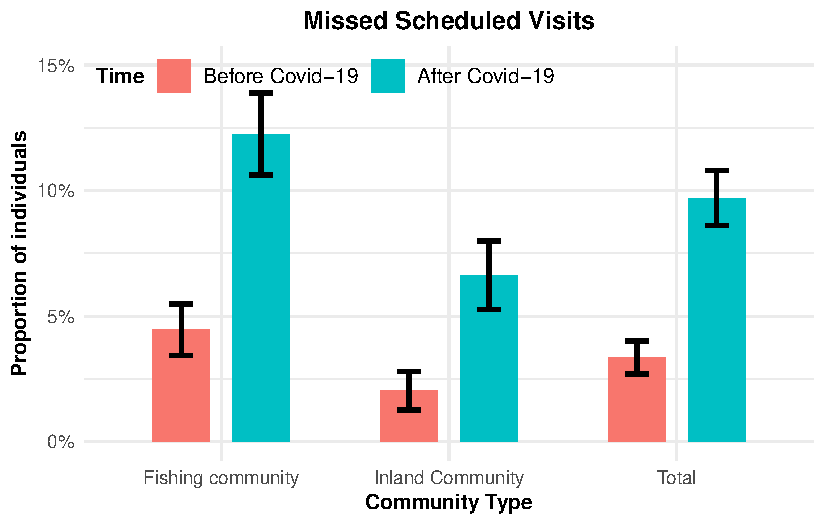
\includegraphics[keepaspectratio]{Rakai_revision_files/figure-pdf/unnamed-chunk-34-1.pdf}}

\subsubsection{Run out of ART by
Community}\label{run-out-of-art-by-community}

\begin{Shaded}
\begin{Highlighting}[]
\NormalTok{df\_com }\SpecialCharTok{\%\textgreater{}\%} \FunctionTok{group\_by}\NormalTok{(community\_type,artrunbc) }\SpecialCharTok{\%\textgreater{}\%} 
  \FunctionTok{count}\NormalTok{()}
\end{Highlighting}
\end{Shaded}

\begin{longtable}[]{@{}llr@{}}
\toprule\noalign{}
community\_type & artrunbc & n \\
\midrule\noalign{}
\endhead
\bottomrule\noalign{}
\endlastfoot
Inland Community & No & 1253 \\
Inland Community & Yes & 30 \\
Fishing community & No & 1514 \\
Fishing community & Yes & 37 \\
\end{longtable}

\begin{Shaded}
\begin{Highlighting}[]
\NormalTok{df\_com }\SpecialCharTok{\%\textgreater{}\%} \FunctionTok{group\_by}\NormalTok{(community\_type,artrunac) }\SpecialCharTok{\%\textgreater{}\%} 
  \FunctionTok{count}\NormalTok{()}
\end{Highlighting}
\end{Shaded}

\begin{longtable}[]{@{}llr@{}}
\toprule\noalign{}
community\_type & artrunac & n \\
\midrule\noalign{}
\endhead
\bottomrule\noalign{}
\endlastfoot
Inland Community & No & 1225 \\
Inland Community & Yes & 58 \\
Fishing community & No & 1457 \\
Fishing community & Yes & 94 \\
\end{longtable}

\begin{Shaded}
\begin{Highlighting}[]
\NormalTok{df\_com\_artrun }\OtherTok{\textless{}{-}}\NormalTok{ df\_com }\SpecialCharTok{\%\textgreater{}\%}
  \FunctionTok{mutate}\NormalTok{(}
    \AttributeTok{artrunbc =} \FunctionTok{as.character}\NormalTok{(artrunbc),}
    \AttributeTok{artrunac =} \FunctionTok{as.character}\NormalTok{(artrunac)}
\NormalTok{  ) }\SpecialCharTok{\%\textgreater{}\%}
  \FunctionTok{pivot\_longer}\NormalTok{(}
    \AttributeTok{cols =} \FunctionTok{c}\NormalTok{(artrunbc, artrunac),}
    \AttributeTok{names\_to =} \StringTok{"variable"}\NormalTok{,}
    \AttributeTok{values\_to =} \StringTok{"response"}
\NormalTok{  ) }\SpecialCharTok{\%\textgreater{}\%}
  \FunctionTok{mutate}\NormalTok{(}
    \AttributeTok{time =} \FunctionTok{if\_else}\NormalTok{(}\FunctionTok{grepl}\NormalTok{(}\StringTok{"bc$"}\NormalTok{, variable), }\StringTok{"Before Covid{-}19"}\NormalTok{, }\StringTok{"After Covid{-}19"}\NormalTok{)}
\NormalTok{  )}

\NormalTok{df\_com\_artrun\_summary }\OtherTok{\textless{}{-}}\NormalTok{ df\_com\_artrun }\SpecialCharTok{\%\textgreater{}\%}
  \FunctionTok{group\_by}\NormalTok{(time,community\_type) }\SpecialCharTok{\%\textgreater{}\%}
  \FunctionTok{summarise}\NormalTok{(}
    \AttributeTok{n\_yes =} \FunctionTok{sum}\NormalTok{(response }\SpecialCharTok{==} \StringTok{"Yes"}\NormalTok{, }\AttributeTok{na.rm =} \ConstantTok{TRUE}\NormalTok{),}
    \AttributeTok{n =} \FunctionTok{n}\NormalTok{(),}
    \AttributeTok{.groups =} \StringTok{"drop"}
\NormalTok{  )}

\NormalTok{df\_com\_artrun\_totals }\OtherTok{\textless{}{-}}\NormalTok{ df\_com\_artrun }\SpecialCharTok{\%\textgreater{}\%}
  \FunctionTok{group\_by}\NormalTok{(time) }\SpecialCharTok{\%\textgreater{}\%}
  \FunctionTok{summarise}\NormalTok{(}
    \AttributeTok{n\_yes =} \FunctionTok{sum}\NormalTok{(response }\SpecialCharTok{==} \StringTok{"Yes"}\NormalTok{, }\AttributeTok{na.rm =} \ConstantTok{TRUE}\NormalTok{),}
    \AttributeTok{n =} \FunctionTok{n}\NormalTok{(),}
    \AttributeTok{.groups =} \StringTok{"drop"}
\NormalTok{  )}

\NormalTok{df\_com\_artrun\_summary }\OtherTok{\textless{}{-}} \FunctionTok{bind\_rows}\NormalTok{(df\_com\_artrun\_summary, df\_com\_artrun\_totals) }\SpecialCharTok{\%\textgreater{}\%}
  \FunctionTok{mutate}\NormalTok{(}
    \AttributeTok{proportion =}\NormalTok{ n\_yes }\SpecialCharTok{/}\NormalTok{ n,}
    \AttributeTok{se =} \FunctionTok{sqrt}\NormalTok{(proportion }\SpecialCharTok{*}\NormalTok{ (}\DecValTok{1} \SpecialCharTok{{-}}\NormalTok{ proportion) }\SpecialCharTok{/}\NormalTok{ n),}
    \AttributeTok{lower =}\NormalTok{ proportion }\SpecialCharTok{{-}} \FloatTok{1.96} \SpecialCharTok{*}\NormalTok{ se,}
    \AttributeTok{upper =}\NormalTok{ proportion }\SpecialCharTok{+} \FloatTok{1.96} \SpecialCharTok{*}\NormalTok{ se}
\NormalTok{  ) }\SpecialCharTok{\%\textgreater{}\%} 
 \FunctionTok{mutate}\NormalTok{(}\AttributeTok{time =} \FunctionTok{as\_factor}\NormalTok{(time) }\SpecialCharTok{\%\textgreater{}\%} 
           \FunctionTok{fct\_relevel}\NormalTok{(}\StringTok{"Before Covid{-}19"}\NormalTok{),}
         \AttributeTok{community\_type =} \FunctionTok{if\_else}\NormalTok{(}\FunctionTok{is.na}\NormalTok{(community\_type),}\StringTok{"Total"}\NormalTok{,community\_type))}




  
\NormalTok{df\_com\_artrun\_summary}
\end{Highlighting}
\end{Shaded}

\begin{longtable}[]{@{}
  >{\raggedright\arraybackslash}p{(\linewidth - 14\tabcolsep) * \real{0.1860}}
  >{\raggedright\arraybackslash}p{(\linewidth - 14\tabcolsep) * \real{0.2093}}
  >{\raggedleft\arraybackslash}p{(\linewidth - 14\tabcolsep) * \real{0.0698}}
  >{\raggedleft\arraybackslash}p{(\linewidth - 14\tabcolsep) * \real{0.0581}}
  >{\raggedleft\arraybackslash}p{(\linewidth - 14\tabcolsep) * \real{0.1279}}
  >{\raggedleft\arraybackslash}p{(\linewidth - 14\tabcolsep) * \real{0.1163}}
  >{\raggedleft\arraybackslash}p{(\linewidth - 14\tabcolsep) * \real{0.1163}}
  >{\raggedleft\arraybackslash}p{(\linewidth - 14\tabcolsep) * \real{0.1163}}@{}}
\toprule\noalign{}
\begin{minipage}[b]{\linewidth}\raggedright
time
\end{minipage} & \begin{minipage}[b]{\linewidth}\raggedright
community\_type
\end{minipage} & \begin{minipage}[b]{\linewidth}\raggedleft
n\_yes
\end{minipage} & \begin{minipage}[b]{\linewidth}\raggedleft
n
\end{minipage} & \begin{minipage}[b]{\linewidth}\raggedleft
proportion
\end{minipage} & \begin{minipage}[b]{\linewidth}\raggedleft
se
\end{minipage} & \begin{minipage}[b]{\linewidth}\raggedleft
lower
\end{minipage} & \begin{minipage}[b]{\linewidth}\raggedleft
upper
\end{minipage} \\
\midrule\noalign{}
\endhead
\bottomrule\noalign{}
\endlastfoot
After Covid-19 & Inland Community & 58 & 1283 & 0.0452065 & 0.0058002 &
0.0338382 & 0.0565749 \\
After Covid-19 & Fishing community & 94 & 1551 & 0.0606061 & 0.0060587 &
0.0487311 & 0.0724810 \\
Before Covid-19 & Inland Community & 30 & 1283 & 0.0233827 & 0.0042189 &
0.0151137 & 0.0316517 \\
Before Covid-19 & Fishing community & 37 & 1551 & 0.0238556 & 0.0038748
& 0.0162610 & 0.0314501 \\
After Covid-19 & Total & 152 & 2834 & 0.0536344 & 0.0042321 & 0.0453396
& 0.0619293 \\
Before Covid-19 & Total & 67 & 2834 & 0.0236415 & 0.0028539 & 0.0180478
& 0.0292352 \\
\end{longtable}

\begin{Shaded}
\begin{Highlighting}[]
\NormalTok{run\_out\_of\_art\_by\_community\_plot }\OtherTok{\textless{}{-}} \FunctionTok{ggplot}\NormalTok{(df\_com\_artrun\_summary, }\FunctionTok{aes}\NormalTok{(}\AttributeTok{x =}\NormalTok{ community\_type, }\AttributeTok{y =}\NormalTok{ proportion, }\AttributeTok{fill =}\NormalTok{ time)) }\SpecialCharTok{+}
  \FunctionTok{geom\_col}\NormalTok{(}\AttributeTok{position =} \FunctionTok{position\_dodge}\NormalTok{(}\AttributeTok{width =} \FloatTok{0.7}\NormalTok{), }\AttributeTok{width =} \FloatTok{0.5}\NormalTok{) }\SpecialCharTok{+}
  \FunctionTok{geom\_errorbar}\NormalTok{(}
    \FunctionTok{aes}\NormalTok{(}\AttributeTok{ymin =}\NormalTok{ lower, }\AttributeTok{ymax =}\NormalTok{ upper),}
    \AttributeTok{position =} \FunctionTok{position\_dodge}\NormalTok{(}\AttributeTok{width =} \FloatTok{0.7}\NormalTok{),}
    \AttributeTok{width =} \FloatTok{0.2}\NormalTok{,}
    \AttributeTok{size =} \DecValTok{1}
\NormalTok{  ) }\SpecialCharTok{+}
  \FunctionTok{scale\_y\_continuous}\NormalTok{(}\AttributeTok{labels =}\NormalTok{ scales}\SpecialCharTok{::}\FunctionTok{percent\_format}\NormalTok{(}\AttributeTok{accuracy =} \DecValTok{1}\NormalTok{),}\AttributeTok{limits =} \FunctionTok{c}\NormalTok{(}\DecValTok{0}\NormalTok{, }\FloatTok{0.12}\NormalTok{)) }\SpecialCharTok{+}
  \FunctionTok{labs}\NormalTok{(}
    \AttributeTok{title =} \StringTok{"Run Out of ART"}\NormalTok{,}
    \AttributeTok{x =} \StringTok{"Community Type"}\NormalTok{,}
    \AttributeTok{y =} \StringTok{"Proportion of individuals"}\NormalTok{,}
    \AttributeTok{fill =} \StringTok{"Time"}
\NormalTok{  ) }\SpecialCharTok{+}
  \FunctionTok{theme\_minimal}\NormalTok{() }\SpecialCharTok{+}
  \FunctionTok{theme}\NormalTok{(}
    \AttributeTok{plot.title =} \FunctionTok{element\_text}\NormalTok{(}\AttributeTok{hjust =} \FloatTok{0.5}\NormalTok{, }\AttributeTok{face =} \StringTok{"bold"}\NormalTok{, }\AttributeTok{size =} \DecValTok{12}\NormalTok{),}
    \AttributeTok{axis.title.x =} \FunctionTok{element\_text}\NormalTok{(}\AttributeTok{face =} \StringTok{"bold"}\NormalTok{, }\AttributeTok{size =} \DecValTok{10}\NormalTok{),}
    \AttributeTok{axis.title.y =} \FunctionTok{element\_text}\NormalTok{(}\AttributeTok{face =} \StringTok{"bold"}\NormalTok{, }\AttributeTok{size =} \DecValTok{10}\NormalTok{),}
    \AttributeTok{legend.title =} \FunctionTok{element\_text}\NormalTok{(}\AttributeTok{face =} \StringTok{"bold"}\NormalTok{, }\AttributeTok{size =} \DecValTok{10}\NormalTok{),}
    \AttributeTok{legend.text =} \FunctionTok{element\_text}\NormalTok{(}\AttributeTok{size =} \DecValTok{10}\NormalTok{),}
    \AttributeTok{legend.position =} \FunctionTok{c}\NormalTok{(}\DecValTok{0}\NormalTok{, }\DecValTok{1}\NormalTok{),}
    \AttributeTok{legend.justification =} \FunctionTok{c}\NormalTok{(}\DecValTok{0}\NormalTok{, }\DecValTok{1}\NormalTok{),}
    \AttributeTok{legend.direction =} \StringTok{"horizontal"}
\NormalTok{  )}
\NormalTok{run\_out\_of\_art\_by\_community\_plot}
\end{Highlighting}
\end{Shaded}

\pandocbounded{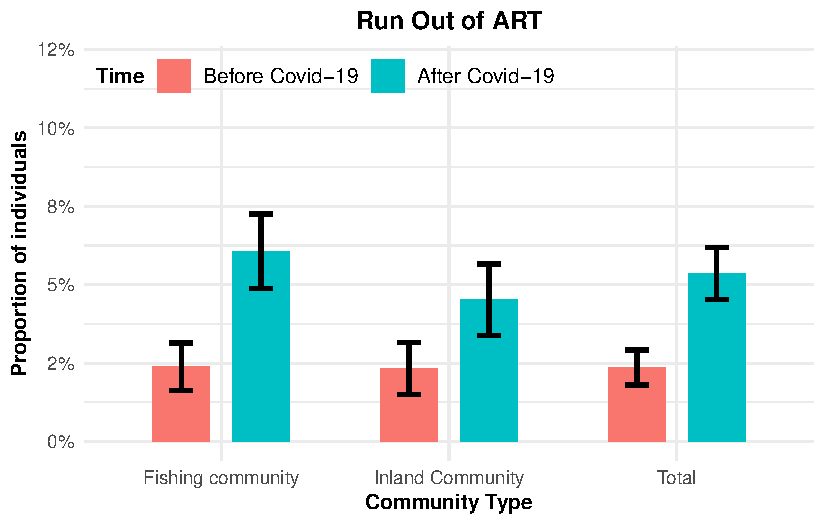
\includegraphics[keepaspectratio]{Rakai_revision_files/figure-pdf/unnamed-chunk-37-1.pdf}}

\begin{Shaded}
\begin{Highlighting}[]
\NormalTok{pc1 }\OtherTok{\textless{}{-}} \FunctionTok{ggplot}\NormalTok{(df\_com\_artstr\_summary, }\FunctionTok{aes}\NormalTok{(}\AttributeTok{x =}\NormalTok{ community\_type, }\AttributeTok{y =}\NormalTok{ proportion, }\AttributeTok{fill =}\NormalTok{time)) }\SpecialCharTok{+}
  \FunctionTok{geom\_col}\NormalTok{(}\AttributeTok{position =} \FunctionTok{position\_dodge}\NormalTok{(}\AttributeTok{width =} \FloatTok{0.7}\NormalTok{), }\AttributeTok{width =} \FloatTok{0.5}\NormalTok{) }\SpecialCharTok{+}
  \FunctionTok{geom\_errorbar}\NormalTok{(}
    \FunctionTok{aes}\NormalTok{(}\AttributeTok{ymin =}\NormalTok{ lower, }\AttributeTok{ymax =}\NormalTok{ upper),}
    \AttributeTok{position =} \FunctionTok{position\_dodge}\NormalTok{(}\AttributeTok{width =} \FloatTok{0.7}\NormalTok{),}
    \AttributeTok{width =} \FloatTok{0.2}\NormalTok{,}
    \AttributeTok{size =} \DecValTok{1}
\NormalTok{  ) }\SpecialCharTok{+}
  \FunctionTok{scale\_y\_continuous}\NormalTok{(}\AttributeTok{labels =}\NormalTok{ scales}\SpecialCharTok{::}\FunctionTok{percent\_format}\NormalTok{(}\AttributeTok{accuracy =} \DecValTok{1}\NormalTok{),}\AttributeTok{limits =} \FunctionTok{c}\NormalTok{(}\DecValTok{0}\NormalTok{, }\FloatTok{0.25}\NormalTok{)) }\SpecialCharTok{+}
  \FunctionTok{labs}\NormalTok{(}
    \AttributeTok{title =} \StringTok{"Reduced ART Intake"}\NormalTok{,}
    \AttributeTok{x =} \StringTok{"Community Type"}\NormalTok{,}
    \AttributeTok{y =} \StringTok{"Proportion of individuals"}\NormalTok{,}
    \AttributeTok{fill =} \StringTok{"Time"}
\NormalTok{  ) }\SpecialCharTok{+}
  \FunctionTok{theme\_minimal}\NormalTok{() }\SpecialCharTok{+}
  \FunctionTok{theme}\NormalTok{(}
    \AttributeTok{plot.title =} \FunctionTok{element\_text}\NormalTok{(}\AttributeTok{hjust =} \FloatTok{0.5}\NormalTok{, }\AttributeTok{face =} \StringTok{"bold"}\NormalTok{, }\AttributeTok{size =} \DecValTok{12}\NormalTok{),}
    \AttributeTok{axis.title.x =} \FunctionTok{element\_text}\NormalTok{(}\AttributeTok{face =} \StringTok{"bold"}\NormalTok{, }\AttributeTok{size =} \DecValTok{10}\NormalTok{),}
    \AttributeTok{axis.title.y =} \FunctionTok{element\_text}\NormalTok{(}\AttributeTok{face =} \StringTok{"bold"}\NormalTok{, }\AttributeTok{size =} \DecValTok{10}\NormalTok{),}
    \AttributeTok{legend.title =} \FunctionTok{element\_text}\NormalTok{(}\AttributeTok{face =} \StringTok{"bold"}\NormalTok{, }\AttributeTok{size =} \DecValTok{10}\NormalTok{),}
    \AttributeTok{legend.text =} \FunctionTok{element\_text}\NormalTok{(}\AttributeTok{size =} \DecValTok{10}\NormalTok{),}
    \AttributeTok{legend.position =} \FunctionTok{c}\NormalTok{(}\DecValTok{0}\NormalTok{, }\DecValTok{1}\NormalTok{),}
    \AttributeTok{legend.justification =} \FunctionTok{c}\NormalTok{(}\DecValTok{0}\NormalTok{, }\DecValTok{1}\NormalTok{),}
    \AttributeTok{legend.direction =} \StringTok{"horizontal"}
\NormalTok{  )}
\NormalTok{pc1 }\DocumentationTok{\#\# }
\end{Highlighting}
\end{Shaded}

\pandocbounded{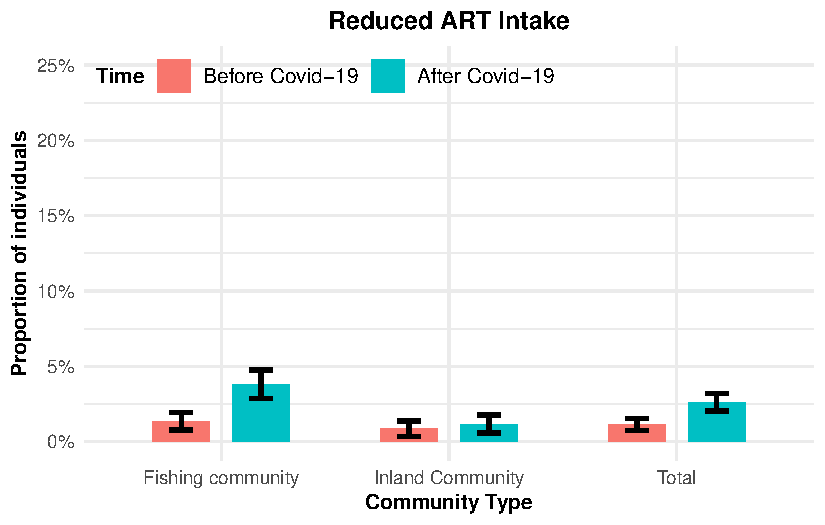
\includegraphics[keepaspectratio]{Rakai_revision_files/figure-pdf/unnamed-chunk-38-1.pdf}}

\begin{Shaded}
\begin{Highlighting}[]
\NormalTok{pc2 }\OtherTok{\textless{}{-}} \FunctionTok{ggplot}\NormalTok{(df\_com\_hiv\_summary, }\FunctionTok{aes}\NormalTok{(}\AttributeTok{x =}\NormalTok{ community\_type, }\AttributeTok{y =}\NormalTok{ proportion, }\AttributeTok{fill =}\NormalTok{ time)) }\SpecialCharTok{+}
  \FunctionTok{geom\_col}\NormalTok{(}\AttributeTok{position =} \FunctionTok{position\_dodge}\NormalTok{(}\AttributeTok{width =} \FloatTok{0.7}\NormalTok{), }\AttributeTok{width =} \FloatTok{0.5}\NormalTok{) }\SpecialCharTok{+}
  \FunctionTok{geom\_errorbar}\NormalTok{(}
    \FunctionTok{aes}\NormalTok{(}\AttributeTok{ymin =}\NormalTok{ lower, }\AttributeTok{ymax =}\NormalTok{ upper),}
    \AttributeTok{position =} \FunctionTok{position\_dodge}\NormalTok{(}\AttributeTok{width =} \FloatTok{0.7}\NormalTok{),}
    \AttributeTok{width =} \FloatTok{0.2}\NormalTok{,}
    \AttributeTok{size =} \DecValTok{1}
\NormalTok{  ) }\SpecialCharTok{+}
  \FunctionTok{scale\_y\_continuous}\NormalTok{(}\AttributeTok{labels =}\NormalTok{ scales}\SpecialCharTok{::}\FunctionTok{percent\_format}\NormalTok{(}\AttributeTok{accuracy =} \DecValTok{1}\NormalTok{),}\AttributeTok{limits =} \FunctionTok{c}\NormalTok{(}\DecValTok{0}\NormalTok{, }\FloatTok{0.25}\NormalTok{)) }\SpecialCharTok{+}
  \FunctionTok{labs}\NormalTok{(}
    \AttributeTok{title =} \StringTok{"Missed Scheduled Visits"}\NormalTok{,}
    \AttributeTok{x =} \StringTok{"Community Type"}\NormalTok{,}
    \AttributeTok{y =} \StringTok{"Proportion of individuals"}\NormalTok{,}
    \AttributeTok{fill =} \StringTok{"Time"}
\NormalTok{  ) }\SpecialCharTok{+}
  \FunctionTok{theme\_minimal}\NormalTok{() }\SpecialCharTok{+}
  \FunctionTok{theme}\NormalTok{(}
    \AttributeTok{plot.title =} \FunctionTok{element\_text}\NormalTok{(}\AttributeTok{hjust =} \FloatTok{0.5}\NormalTok{, }\AttributeTok{face =} \StringTok{"bold"}\NormalTok{, }\AttributeTok{size =} \DecValTok{12}\NormalTok{),}
    \AttributeTok{axis.title.x =} \FunctionTok{element\_text}\NormalTok{(}\AttributeTok{face =} \StringTok{"bold"}\NormalTok{, }\AttributeTok{size =} \DecValTok{10}\NormalTok{),}
    \AttributeTok{axis.title.y =} \FunctionTok{element\_text}\NormalTok{(}\AttributeTok{face =} \StringTok{"bold"}\NormalTok{, }\AttributeTok{size =} \DecValTok{10}\NormalTok{),}
    \AttributeTok{legend.title =} \FunctionTok{element\_text}\NormalTok{(}\AttributeTok{face =} \StringTok{"bold"}\NormalTok{, }\AttributeTok{size =} \DecValTok{10}\NormalTok{),}
    \AttributeTok{legend.text =} \FunctionTok{element\_text}\NormalTok{(}\AttributeTok{size =} \DecValTok{10}\NormalTok{),}
    \AttributeTok{legend.position =} \FunctionTok{c}\NormalTok{(}\DecValTok{0}\NormalTok{, }\DecValTok{1}\NormalTok{),}
    \AttributeTok{legend.justification =} \FunctionTok{c}\NormalTok{(}\DecValTok{0}\NormalTok{, }\DecValTok{1}\NormalTok{),}
    \AttributeTok{legend.direction =} \StringTok{"horizontal"}
\NormalTok{  )}
\NormalTok{pc2 }\DocumentationTok{\#\# Missed scheduled visits}
\end{Highlighting}
\end{Shaded}

\pandocbounded{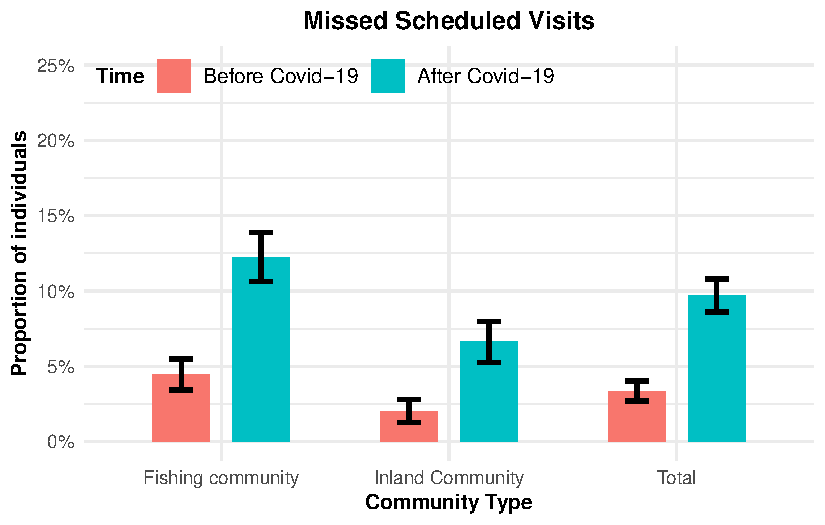
\includegraphics[keepaspectratio]{Rakai_revision_files/figure-pdf/unnamed-chunk-39-1.pdf}}

\begin{Shaded}
\begin{Highlighting}[]
\DocumentationTok{\#\# Run out of pills}
\NormalTok{pc3 }\OtherTok{\textless{}{-}} \FunctionTok{ggplot}\NormalTok{(df\_com\_artrun\_summary, }\FunctionTok{aes}\NormalTok{(}\AttributeTok{x =}\NormalTok{ community\_type, }\AttributeTok{y =}\NormalTok{ proportion, }\AttributeTok{fill =}\NormalTok{time)) }\SpecialCharTok{+}
  \FunctionTok{geom\_col}\NormalTok{(}\AttributeTok{position =} \FunctionTok{position\_dodge}\NormalTok{(}\AttributeTok{width =} \FloatTok{0.7}\NormalTok{), }\AttributeTok{width =} \FloatTok{0.5}\NormalTok{) }\SpecialCharTok{+}
  \FunctionTok{geom\_errorbar}\NormalTok{(}
    \FunctionTok{aes}\NormalTok{(}\AttributeTok{ymin =}\NormalTok{ lower, }\AttributeTok{ymax =}\NormalTok{ upper),}
    \AttributeTok{position =} \FunctionTok{position\_dodge}\NormalTok{(}\AttributeTok{width =} \FloatTok{0.7}\NormalTok{),}
    \AttributeTok{width =} \FloatTok{0.2}\NormalTok{,}
    \AttributeTok{size =} \DecValTok{1}
\NormalTok{  ) }\SpecialCharTok{+}
  \FunctionTok{scale\_y\_continuous}\NormalTok{(}\AttributeTok{labels =}\NormalTok{ scales}\SpecialCharTok{::}\FunctionTok{percent\_format}\NormalTok{(}\AttributeTok{accuracy =} \DecValTok{1}\NormalTok{),}\AttributeTok{limits =} \FunctionTok{c}\NormalTok{(}\DecValTok{0}\NormalTok{, }\FloatTok{0.25}\NormalTok{)) }\SpecialCharTok{+}
  \FunctionTok{labs}\NormalTok{(}
    \AttributeTok{title =}  \StringTok{"Run Out of ART"}\NormalTok{,}
    \AttributeTok{x =} \StringTok{"Community Type"}\NormalTok{,}
    \AttributeTok{y =} \StringTok{"Proportion of individuals"}\NormalTok{,}
    \AttributeTok{fill =} \StringTok{"Time"}
\NormalTok{  ) }\SpecialCharTok{+}
  \FunctionTok{theme\_minimal}\NormalTok{() }\SpecialCharTok{+}
  \FunctionTok{theme}\NormalTok{(}
    \AttributeTok{plot.title =}  \FunctionTok{element\_text}\NormalTok{(}\AttributeTok{hjust =} \FloatTok{0.5}\NormalTok{, }\AttributeTok{face =} \StringTok{"bold"}\NormalTok{, }\AttributeTok{size =} \DecValTok{12}\NormalTok{),}
    \AttributeTok{axis.title.x =} \FunctionTok{element\_text}\NormalTok{(}\AttributeTok{face =} \StringTok{"bold"}\NormalTok{, }\AttributeTok{size =} \DecValTok{10}\NormalTok{),}
    \AttributeTok{axis.title.y =} \FunctionTok{element\_text}\NormalTok{(}\AttributeTok{face =} \StringTok{"bold"}\NormalTok{, }\AttributeTok{size =} \DecValTok{10}\NormalTok{),}
    \AttributeTok{legend.title =} \FunctionTok{element\_text}\NormalTok{(}\AttributeTok{face =} \StringTok{"bold"}\NormalTok{, }\AttributeTok{size =} \DecValTok{10}\NormalTok{),}
    \AttributeTok{legend.text =} \FunctionTok{element\_text}\NormalTok{(}\AttributeTok{size =} \DecValTok{10}\NormalTok{),}
    \AttributeTok{legend.position =} \FunctionTok{c}\NormalTok{(}\DecValTok{0}\NormalTok{, }\DecValTok{1}\NormalTok{),}
    \AttributeTok{legend.justification =} \FunctionTok{c}\NormalTok{(}\DecValTok{0}\NormalTok{, }\DecValTok{1}\NormalTok{),}
    \AttributeTok{legend.direction =} \StringTok{"horizontal"}
\NormalTok{  )}

\NormalTok{pc3}
\end{Highlighting}
\end{Shaded}

\pandocbounded{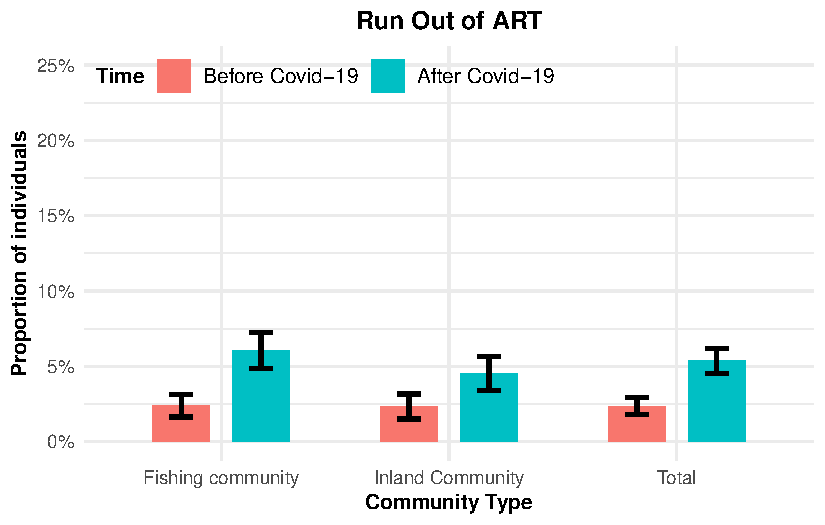
\includegraphics[keepaspectratio]{Rakai_revision_files/figure-pdf/unnamed-chunk-40-1.pdf}}

\begin{Shaded}
\begin{Highlighting}[]
\DocumentationTok{\#\#\# Combined plot}
\NormalTok{(pc1 }\SpecialCharTok{+}\NormalTok{ pc2)}\SpecialCharTok{/}\NormalTok{pc3}
\end{Highlighting}
\end{Shaded}

\pandocbounded{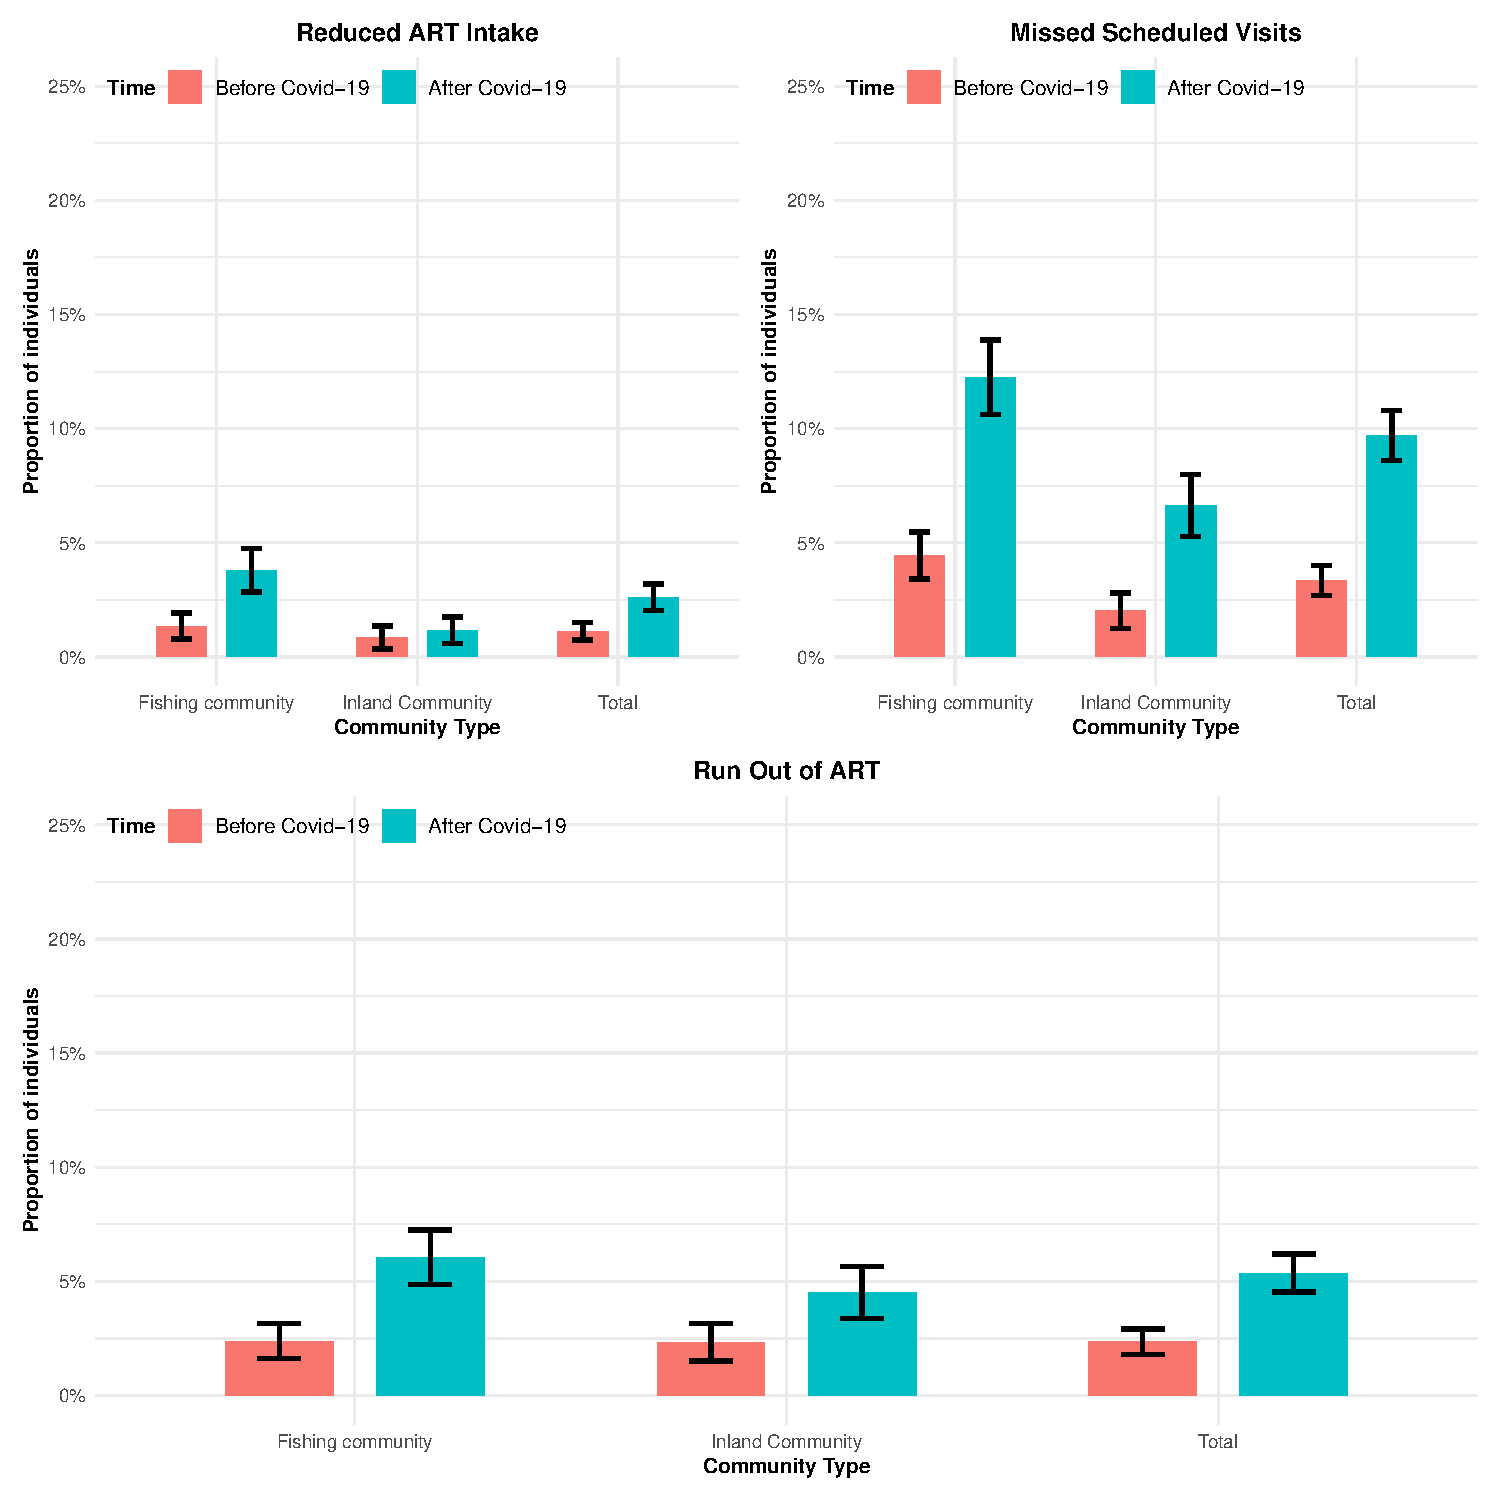
\includegraphics[keepaspectratio]{Rakai_revision_files/figure-pdf/unnamed-chunk-41-1.pdf}}

\subsubsection{Mobility}\label{mobility}

\begin{Shaded}
\begin{Highlighting}[]
\NormalTok{df\_mob }\OtherTok{\textless{}{-}}\NormalTok{  rakai }\SpecialCharTok{\%\textgreater{}\%} 
  \FunctionTok{select}\NormalTok{(mobility,artrunbc,artrunac,}
\NormalTok{         hivac,hivbc,copies,new\_copies,artstrac,artstrbc) }\SpecialCharTok{\%\textgreater{}\%} 
  \FunctionTok{filter}\NormalTok{(hivac }\SpecialCharTok{!=}\DecValTok{8}\NormalTok{, hivbc}\SpecialCharTok{!=}\DecValTok{8}\NormalTok{,artrunbc}\SpecialCharTok{!=}\DecValTok{8}\NormalTok{,artstrac}\SpecialCharTok{!=}\DecValTok{8}\NormalTok{,artstrbc}\SpecialCharTok{!=}\DecValTok{8}\NormalTok{,artrunac}\SpecialCharTok{!=}\DecValTok{8}\NormalTok{) }\SpecialCharTok{\%\textgreater{}\%} 
  \FunctionTok{mutate}\NormalTok{(}
    \AttributeTok{mobility =} \FunctionTok{case\_when}\NormalTok{(}
\NormalTok{           mobility }\SpecialCharTok{\%in\%} \FunctionTok{c}\NormalTok{(}\DecValTok{3}\NormalTok{,}\DecValTok{8}\NormalTok{,}\DecValTok{10}\NormalTok{) }\SpecialCharTok{\textasciitilde{}} \StringTok{"In{-}migrant"}\NormalTok{,}
           \AttributeTok{.default =} \StringTok{"Long{-}term resident"}\NormalTok{) }\SpecialCharTok{\%\textgreater{}\%} 
           \FunctionTok{fct\_relevel}\NormalTok{(}\StringTok{"In{-}migrant"}\NormalTok{) }\SpecialCharTok{\%\textgreater{}\%} 
           \FunctionTok{ff\_label}\NormalTok{(}\StringTok{"Migration"}\NormalTok{),}
  
    \AttributeTok{hivac =} \FunctionTok{if\_else}\NormalTok{(hivac }\SpecialCharTok{==}\DecValTok{1}\NormalTok{, }\StringTok{"Yes"}\NormalTok{,}\StringTok{"No"}\NormalTok{) }\SpecialCharTok{\%\textgreater{}\%} 
    \FunctionTok{ff\_label}\NormalTok{(}\StringTok{"Missed scheduled visit for HIV care"}\NormalTok{) }\SpecialCharTok{\%\textgreater{}\%} 
      \FunctionTok{as\_factor}\NormalTok{(),}
   
     \AttributeTok{hivbc =} \FunctionTok{if\_else}\NormalTok{(hivbc }\SpecialCharTok{==}\DecValTok{1}\NormalTok{,}\StringTok{"Yes"}\NormalTok{,}\StringTok{"No"}\NormalTok{) }\SpecialCharTok{\%\textgreater{}\%} 
    \FunctionTok{ff\_label}\NormalTok{(}\StringTok{"Missed scheduled visit for HIV care"}\NormalTok{) }\SpecialCharTok{\%\textgreater{}\%} 
    \FunctionTok{as\_factor}\NormalTok{(),}
 
     \AttributeTok{artrunac =} \FunctionTok{if\_else}\NormalTok{(artrunac }\SpecialCharTok{==}\DecValTok{1}\NormalTok{,}\StringTok{"Yes"}\NormalTok{,}\StringTok{"No"}\NormalTok{) }\SpecialCharTok{\%\textgreater{}\%} 
    \FunctionTok{as\_factor}\NormalTok{() }\SpecialCharTok{\%\textgreater{}\%} 
    \FunctionTok{ff\_label}\NormalTok{(}\StringTok{"Run out of ART before next refill"}\NormalTok{),}
 
   \AttributeTok{artrunbc =} \FunctionTok{if\_else}\NormalTok{(artrunbc }\SpecialCharTok{==}\DecValTok{1}\NormalTok{,}\StringTok{"Yes"}\NormalTok{,}\StringTok{"No"}\NormalTok{) }\SpecialCharTok{\%\textgreater{}\%} 
    \FunctionTok{as\_factor}\NormalTok{() }\SpecialCharTok{\%\textgreater{}\%} 
    \FunctionTok{ff\_label}\NormalTok{(}\StringTok{"Run out of ART before next refill"}\NormalTok{),}
  
  \AttributeTok{artstrac =} \FunctionTok{if\_else}\NormalTok{(artstrac }\SpecialCharTok{==}\DecValTok{1}\NormalTok{,}\StringTok{"Yes"}\NormalTok{,}\StringTok{"No"}\NormalTok{) }\SpecialCharTok{\%\textgreater{}\%} 
    \FunctionTok{as\_factor}\NormalTok{() }\SpecialCharTok{\%\textgreater{}\%} 
    \FunctionTok{ff\_label}\NormalTok{(}\StringTok{"Taken ART pills less frequently / in smaller}
\StringTok{amounts to conserve supply"}\NormalTok{),}
  
  \AttributeTok{artstrbc =} \FunctionTok{if\_else}\NormalTok{(artstrbc }\SpecialCharTok{==}\DecValTok{1}\NormalTok{,}\StringTok{"Yes"}\NormalTok{,}\StringTok{"No"}\NormalTok{) }\SpecialCharTok{\%\textgreater{}\%} 
    \FunctionTok{as\_factor}\NormalTok{() }\SpecialCharTok{\%\textgreater{}\%} 
    \FunctionTok{ff\_label}\NormalTok{(}\StringTok{"Taken ART pills less frequently / in smaller}
\StringTok{amounts to conserve supply"}\NormalTok{)}
\NormalTok{  )}
\end{Highlighting}
\end{Shaded}

\subsubsection{Run Out of ART by
mobility}\label{run-out-of-art-by-mobility}

\begin{Shaded}
\begin{Highlighting}[]
\NormalTok{df\_mob }\SpecialCharTok{\%\textgreater{}\%} \FunctionTok{group\_by}\NormalTok{(mobility,artrunbc) }\SpecialCharTok{\%\textgreater{}\%} 
  \FunctionTok{count}\NormalTok{()}
\end{Highlighting}
\end{Shaded}

\begin{longtable}[]{@{}llr@{}}
\toprule\noalign{}
mobility & artrunbc & n \\
\midrule\noalign{}
\endhead
\bottomrule\noalign{}
\endlastfoot
In-migrant & No & 610 \\
In-migrant & Yes & 22 \\
Long-term resident & No & 2157 \\
Long-term resident & Yes & 45 \\
\end{longtable}

\begin{Shaded}
\begin{Highlighting}[]
\NormalTok{df\_mob }\SpecialCharTok{\%\textgreater{}\%} \FunctionTok{group\_by}\NormalTok{(mobility,artrunac) }\SpecialCharTok{\%\textgreater{}\%} 
  \FunctionTok{count}\NormalTok{()}
\end{Highlighting}
\end{Shaded}

\begin{longtable}[]{@{}llr@{}}
\toprule\noalign{}
mobility & artrunac & n \\
\midrule\noalign{}
\endhead
\bottomrule\noalign{}
\endlastfoot
In-migrant & No & 582 \\
In-migrant & Yes & 50 \\
Long-term resident & No & 2100 \\
Long-term resident & Yes & 102 \\
\end{longtable}

\begin{Shaded}
\begin{Highlighting}[]
\NormalTok{df\_mob\_artrun }\OtherTok{\textless{}{-}}\NormalTok{ df\_mob }\SpecialCharTok{\%\textgreater{}\%}
  \FunctionTok{mutate}\NormalTok{(}
    \AttributeTok{artrunbc =} \FunctionTok{as.character}\NormalTok{(artrunbc),}
    \AttributeTok{artrunac =} \FunctionTok{as.character}\NormalTok{(artrunac)}
\NormalTok{  ) }\SpecialCharTok{\%\textgreater{}\%}
  \FunctionTok{pivot\_longer}\NormalTok{(}
    \AttributeTok{cols =} \FunctionTok{c}\NormalTok{(artrunbc, artrunac),}
    \AttributeTok{names\_to =} \StringTok{"variable"}\NormalTok{,}
    \AttributeTok{values\_to =} \StringTok{"response"}
\NormalTok{  ) }\SpecialCharTok{\%\textgreater{}\%}
  \FunctionTok{mutate}\NormalTok{(}
    \AttributeTok{time =} \FunctionTok{if\_else}\NormalTok{(}\FunctionTok{grepl}\NormalTok{(}\StringTok{"bc$"}\NormalTok{, variable), }\StringTok{"Before Covid{-}19"}\NormalTok{, }\StringTok{"After Covid{-}19"}\NormalTok{)}
\NormalTok{  )}

\NormalTok{df\_mob\_artrun\_summary }\OtherTok{\textless{}{-}}\NormalTok{ df\_mob\_artrun }\SpecialCharTok{\%\textgreater{}\%}
  \FunctionTok{group\_by}\NormalTok{(time,mobility) }\SpecialCharTok{\%\textgreater{}\%}
  \FunctionTok{summarise}\NormalTok{(}
    \AttributeTok{n\_yes =} \FunctionTok{sum}\NormalTok{(response }\SpecialCharTok{==} \StringTok{"Yes"}\NormalTok{, }\AttributeTok{na.rm =} \ConstantTok{TRUE}\NormalTok{),}
    \AttributeTok{n =} \FunctionTok{n}\NormalTok{(),}
    \AttributeTok{.groups =} \StringTok{"drop"}
\NormalTok{  )}

\NormalTok{df\_mob\_artrun\_totals }\OtherTok{\textless{}{-}}\NormalTok{ df\_mob\_artrun }\SpecialCharTok{\%\textgreater{}\%}
  \FunctionTok{group\_by}\NormalTok{(time) }\SpecialCharTok{\%\textgreater{}\%}
  \FunctionTok{summarise}\NormalTok{(}
    \AttributeTok{n\_yes =} \FunctionTok{sum}\NormalTok{(response }\SpecialCharTok{==} \StringTok{"Yes"}\NormalTok{, }\AttributeTok{na.rm =} \ConstantTok{TRUE}\NormalTok{),}
    \AttributeTok{n =} \FunctionTok{n}\NormalTok{(),}
    \AttributeTok{.groups =} \StringTok{"drop"}
\NormalTok{  )}

\NormalTok{df\_mob\_artrun\_summary }\OtherTok{\textless{}{-}} \FunctionTok{bind\_rows}\NormalTok{(df\_mob\_artrun\_summary, df\_mob\_artrun\_totals) }\SpecialCharTok{\%\textgreater{}\%}
  \FunctionTok{mutate}\NormalTok{(}
    \AttributeTok{proportion =}\NormalTok{ n\_yes }\SpecialCharTok{/}\NormalTok{ n,}
    \AttributeTok{se =} \FunctionTok{sqrt}\NormalTok{(proportion }\SpecialCharTok{*}\NormalTok{ (}\DecValTok{1} \SpecialCharTok{{-}}\NormalTok{ proportion) }\SpecialCharTok{/}\NormalTok{ n),}
    \AttributeTok{lower =}\NormalTok{ proportion }\SpecialCharTok{{-}} \FloatTok{1.96} \SpecialCharTok{*}\NormalTok{ se,}
    \AttributeTok{upper =}\NormalTok{ proportion }\SpecialCharTok{+} \FloatTok{1.96} \SpecialCharTok{*}\NormalTok{ se}
\NormalTok{  ) }\SpecialCharTok{\%\textgreater{}\%} 
 \FunctionTok{mutate}\NormalTok{(}\AttributeTok{time =} \FunctionTok{as\_factor}\NormalTok{(time) }\SpecialCharTok{\%\textgreater{}\%} 
           \FunctionTok{fct\_relevel}\NormalTok{(}\StringTok{"Before Covid{-}19"}\NormalTok{),}
         \AttributeTok{mobility =} \FunctionTok{if\_else}\NormalTok{(}\FunctionTok{is.na}\NormalTok{(mobility),}\StringTok{"Total"}\NormalTok{,mobility))}




  
\NormalTok{df\_mob\_artrun\_summary}
\end{Highlighting}
\end{Shaded}

\begin{longtable}[]{@{}
  >{\raggedright\arraybackslash}p{(\linewidth - 14\tabcolsep) * \real{0.1839}}
  >{\raggedright\arraybackslash}p{(\linewidth - 14\tabcolsep) * \real{0.2184}}
  >{\raggedleft\arraybackslash}p{(\linewidth - 14\tabcolsep) * \real{0.0690}}
  >{\raggedleft\arraybackslash}p{(\linewidth - 14\tabcolsep) * \real{0.0575}}
  >{\raggedleft\arraybackslash}p{(\linewidth - 14\tabcolsep) * \real{0.1264}}
  >{\raggedleft\arraybackslash}p{(\linewidth - 14\tabcolsep) * \real{0.1149}}
  >{\raggedleft\arraybackslash}p{(\linewidth - 14\tabcolsep) * \real{0.1149}}
  >{\raggedleft\arraybackslash}p{(\linewidth - 14\tabcolsep) * \real{0.1149}}@{}}
\toprule\noalign{}
\begin{minipage}[b]{\linewidth}\raggedright
time
\end{minipage} & \begin{minipage}[b]{\linewidth}\raggedright
mobility
\end{minipage} & \begin{minipage}[b]{\linewidth}\raggedleft
n\_yes
\end{minipage} & \begin{minipage}[b]{\linewidth}\raggedleft
n
\end{minipage} & \begin{minipage}[b]{\linewidth}\raggedleft
proportion
\end{minipage} & \begin{minipage}[b]{\linewidth}\raggedleft
se
\end{minipage} & \begin{minipage}[b]{\linewidth}\raggedleft
lower
\end{minipage} & \begin{minipage}[b]{\linewidth}\raggedleft
upper
\end{minipage} \\
\midrule\noalign{}
\endhead
\bottomrule\noalign{}
\endlastfoot
After Covid-19 & In-migrant & 50 & 632 & 0.0791139 & 0.0107367 &
0.0580700 & 0.1001579 \\
After Covid-19 & Long-term resident & 102 & 2202 & 0.0463215 & 0.0044790
& 0.0375426 & 0.0551004 \\
Before Covid-19 & In-migrant & 22 & 632 & 0.0348101 & 0.0072912 &
0.0205193 & 0.0491009 \\
Before Covid-19 & Long-term resident & 45 & 2202 & 0.0204360 & 0.0030151
& 0.0145263 & 0.0263456 \\
After Covid-19 & Total & 152 & 2834 & 0.0536344 & 0.0042321 & 0.0453396
& 0.0619293 \\
Before Covid-19 & Total & 67 & 2834 & 0.0236415 & 0.0028539 & 0.0180478
& 0.0292352 \\
\end{longtable}

\begin{Shaded}
\begin{Highlighting}[]
\NormalTok{run\_out\_of\_art\_by\_mobility\_plot }\OtherTok{\textless{}{-}} \FunctionTok{ggplot}\NormalTok{(df\_mob\_artrun\_summary, }\FunctionTok{aes}\NormalTok{(}\AttributeTok{x =}\NormalTok{ mobility, }\AttributeTok{y =}\NormalTok{ proportion, }\AttributeTok{fill =}\NormalTok{ time)) }\SpecialCharTok{+}
  \FunctionTok{geom\_col}\NormalTok{(}\AttributeTok{position =} \FunctionTok{position\_dodge}\NormalTok{(}\AttributeTok{width =} \FloatTok{0.7}\NormalTok{), }\AttributeTok{width =} \FloatTok{0.5}\NormalTok{) }\SpecialCharTok{+}
  \FunctionTok{geom\_errorbar}\NormalTok{(}
    \FunctionTok{aes}\NormalTok{(}\AttributeTok{ymin =}\NormalTok{ lower, }\AttributeTok{ymax =}\NormalTok{ upper),}
    \AttributeTok{position =} \FunctionTok{position\_dodge}\NormalTok{(}\AttributeTok{width =} \FloatTok{0.7}\NormalTok{),}
    \AttributeTok{width =} \FloatTok{0.2}\NormalTok{,}
    \AttributeTok{size =} \DecValTok{1}
\NormalTok{  ) }\SpecialCharTok{+}
  \FunctionTok{scale\_y\_continuous}\NormalTok{(}\AttributeTok{labels =}\NormalTok{ scales}\SpecialCharTok{::}\FunctionTok{percent\_format}\NormalTok{(}\AttributeTok{accuracy =} \DecValTok{1}\NormalTok{),}\AttributeTok{limits =} \FunctionTok{c}\NormalTok{(}\DecValTok{0}\NormalTok{, }\FloatTok{0.12}\NormalTok{)) }\SpecialCharTok{+}
  \FunctionTok{labs}\NormalTok{(}
    \AttributeTok{title =} \StringTok{"Run Out of ART"}\NormalTok{,}
    \AttributeTok{x =} \StringTok{"Mobility"}\NormalTok{,}
    \AttributeTok{y =} \StringTok{"Proportion of individuals"}\NormalTok{,}
    \AttributeTok{fill =} \StringTok{"Time"}
\NormalTok{  ) }\SpecialCharTok{+}
  \FunctionTok{theme\_minimal}\NormalTok{() }\SpecialCharTok{+}
  \FunctionTok{theme}\NormalTok{(}
    \AttributeTok{plot.title =} \FunctionTok{element\_text}\NormalTok{(}\AttributeTok{hjust =} \FloatTok{0.5}\NormalTok{, }\AttributeTok{face =} \StringTok{"bold"}\NormalTok{, }\AttributeTok{size =} \DecValTok{12}\NormalTok{),}
    \AttributeTok{axis.title.x =} \FunctionTok{element\_text}\NormalTok{(}\AttributeTok{face =} \StringTok{"bold"}\NormalTok{, }\AttributeTok{size =} \DecValTok{10}\NormalTok{),}
    \AttributeTok{axis.title.y =} \FunctionTok{element\_text}\NormalTok{(}\AttributeTok{face =} \StringTok{"bold"}\NormalTok{, }\AttributeTok{size =} \DecValTok{10}\NormalTok{),}
    \AttributeTok{legend.title =} \FunctionTok{element\_text}\NormalTok{(}\AttributeTok{face =} \StringTok{"bold"}\NormalTok{, }\AttributeTok{size =} \DecValTok{10}\NormalTok{),}
    \AttributeTok{legend.text =} \FunctionTok{element\_text}\NormalTok{(}\AttributeTok{size =} \DecValTok{10}\NormalTok{),}
    \AttributeTok{legend.position =} \FunctionTok{c}\NormalTok{(}\DecValTok{0}\NormalTok{, }\DecValTok{1}\NormalTok{),}
    \AttributeTok{legend.justification =} \FunctionTok{c}\NormalTok{(}\DecValTok{0}\NormalTok{, }\DecValTok{1}\NormalTok{),}
    \AttributeTok{legend.direction =} \StringTok{"horizontal"}
\NormalTok{  )}
\NormalTok{run\_out\_of\_art\_by\_mobility\_plot}
\end{Highlighting}
\end{Shaded}

\pandocbounded{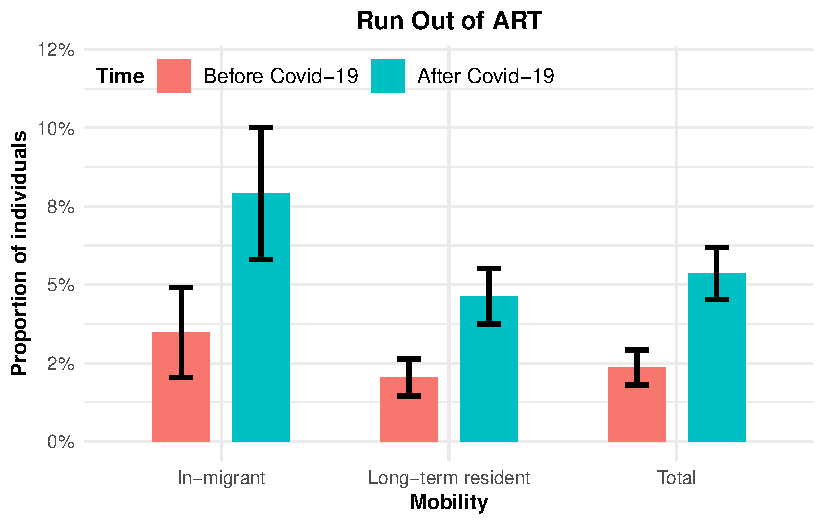
\includegraphics[keepaspectratio]{Rakai_revision_files/figure-pdf/unnamed-chunk-45-1.pdf}}

\subsubsection{reduced ART Intake by
mobility}\label{reduced-art-intake-by-mobility}

\begin{Shaded}
\begin{Highlighting}[]
\NormalTok{df\_mob }\SpecialCharTok{\%\textgreater{}\%} \FunctionTok{group\_by}\NormalTok{(mobility,artstrbc) }\SpecialCharTok{\%\textgreater{}\%} 
  \FunctionTok{count}\NormalTok{()}
\end{Highlighting}
\end{Shaded}

\begin{longtable}[]{@{}llr@{}}
\toprule\noalign{}
mobility & artstrbc & n \\
\midrule\noalign{}
\endhead
\bottomrule\noalign{}
\endlastfoot
In-migrant & No & 625 \\
In-migrant & Yes & 7 \\
Long-term resident & No & 2177 \\
Long-term resident & Yes & 25 \\
\end{longtable}

\begin{Shaded}
\begin{Highlighting}[]
\NormalTok{df\_mob }\SpecialCharTok{\%\textgreater{}\%} \FunctionTok{group\_by}\NormalTok{(mobility,artstrac) }\SpecialCharTok{\%\textgreater{}\%} 
  \FunctionTok{count}\NormalTok{()}
\end{Highlighting}
\end{Shaded}

\begin{longtable}[]{@{}llr@{}}
\toprule\noalign{}
mobility & artstrac & n \\
\midrule\noalign{}
\endhead
\bottomrule\noalign{}
\endlastfoot
In-migrant & No & 611 \\
In-migrant & Yes & 21 \\
Long-term resident & No & 2149 \\
Long-term resident & Yes & 53 \\
\end{longtable}

\begin{Shaded}
\begin{Highlighting}[]
\NormalTok{df\_mob\_artstr }\OtherTok{\textless{}{-}}\NormalTok{ df\_mob }\SpecialCharTok{\%\textgreater{}\%}
  \FunctionTok{pivot\_longer}\NormalTok{(}
    \AttributeTok{cols =} \FunctionTok{c}\NormalTok{(artstrbc, artstrac),}
    \AttributeTok{names\_to =} \StringTok{"variable"}\NormalTok{,}
    \AttributeTok{values\_to =} \StringTok{"response"}
\NormalTok{  ) }\SpecialCharTok{\%\textgreater{}\%}
  \FunctionTok{mutate}\NormalTok{(}
    \AttributeTok{time =} \FunctionTok{if\_else}\NormalTok{(}\FunctionTok{grepl}\NormalTok{(}\StringTok{"bc$"}\NormalTok{, variable), }\StringTok{"Before Covid{-}19"}\NormalTok{, }\StringTok{"After Covid{-}19"}\NormalTok{)}
\NormalTok{  )}

\NormalTok{df\_mob\_artstr\_summary }\OtherTok{\textless{}{-}}\NormalTok{ df\_mob\_artstr }\SpecialCharTok{\%\textgreater{}\%}
  \FunctionTok{group\_by}\NormalTok{(time,mobility) }\SpecialCharTok{\%\textgreater{}\%}
  \FunctionTok{summarise}\NormalTok{(}
    \AttributeTok{n\_yes =} \FunctionTok{sum}\NormalTok{(response }\SpecialCharTok{==} \StringTok{"Yes"}\NormalTok{, }\AttributeTok{na.rm =} \ConstantTok{TRUE}\NormalTok{),}
    \AttributeTok{n =} \FunctionTok{n}\NormalTok{(),}
    \AttributeTok{.groups =} \StringTok{"drop"}
\NormalTok{  )}

\NormalTok{df\_mob\_artstr\_totals }\OtherTok{\textless{}{-}}\NormalTok{ df\_mob\_artstr }\SpecialCharTok{\%\textgreater{}\%}
  \FunctionTok{group\_by}\NormalTok{(time) }\SpecialCharTok{\%\textgreater{}\%}
  \FunctionTok{summarise}\NormalTok{(}
    \AttributeTok{n\_yes =} \FunctionTok{sum}\NormalTok{(response }\SpecialCharTok{==} \StringTok{"Yes"}\NormalTok{, }\AttributeTok{na.rm =} \ConstantTok{TRUE}\NormalTok{),}
    \AttributeTok{n =} \FunctionTok{n}\NormalTok{(),}
    \AttributeTok{.groups =} \StringTok{"drop"}
\NormalTok{  ) }

\NormalTok{df\_mob\_artstr\_summary }\OtherTok{\textless{}{-}} \FunctionTok{bind\_rows}\NormalTok{(df\_mob\_artstr\_summary, df\_mob\_artstr\_totals) }\SpecialCharTok{\%\textgreater{}\%}
  \FunctionTok{mutate}\NormalTok{(}
    \AttributeTok{proportion =}\NormalTok{ n\_yes }\SpecialCharTok{/}\NormalTok{ n,}
    \AttributeTok{se =} \FunctionTok{sqrt}\NormalTok{(proportion }\SpecialCharTok{*}\NormalTok{ (}\DecValTok{1} \SpecialCharTok{{-}}\NormalTok{ proportion) }\SpecialCharTok{/}\NormalTok{ n),}
    \AttributeTok{lower =}\NormalTok{ proportion }\SpecialCharTok{{-}} \FloatTok{1.96} \SpecialCharTok{*}\NormalTok{ se,}
    \AttributeTok{upper =}\NormalTok{ proportion }\SpecialCharTok{+} \FloatTok{1.96} \SpecialCharTok{*}\NormalTok{ se}
\NormalTok{  ) }\SpecialCharTok{\%\textgreater{}\%} 
  \FunctionTok{mutate}\NormalTok{(}\AttributeTok{time =} \FunctionTok{as\_factor}\NormalTok{(time) }\SpecialCharTok{\%\textgreater{}\%} 
           \FunctionTok{fct\_relevel}\NormalTok{(}\StringTok{"Before Covid{-}19"}\NormalTok{),}
         \AttributeTok{mobility =} \FunctionTok{if\_else}\NormalTok{(}\FunctionTok{is.na}\NormalTok{(mobility),}\StringTok{"Total"}\NormalTok{,mobility))}

\NormalTok{df\_mob\_artstr\_summary}
\end{Highlighting}
\end{Shaded}

\begin{longtable}[]{@{}
  >{\raggedright\arraybackslash}p{(\linewidth - 14\tabcolsep) * \real{0.1839}}
  >{\raggedright\arraybackslash}p{(\linewidth - 14\tabcolsep) * \real{0.2184}}
  >{\raggedleft\arraybackslash}p{(\linewidth - 14\tabcolsep) * \real{0.0690}}
  >{\raggedleft\arraybackslash}p{(\linewidth - 14\tabcolsep) * \real{0.0575}}
  >{\raggedleft\arraybackslash}p{(\linewidth - 14\tabcolsep) * \real{0.1264}}
  >{\raggedleft\arraybackslash}p{(\linewidth - 14\tabcolsep) * \real{0.1149}}
  >{\raggedleft\arraybackslash}p{(\linewidth - 14\tabcolsep) * \real{0.1149}}
  >{\raggedleft\arraybackslash}p{(\linewidth - 14\tabcolsep) * \real{0.1149}}@{}}
\toprule\noalign{}
\begin{minipage}[b]{\linewidth}\raggedright
time
\end{minipage} & \begin{minipage}[b]{\linewidth}\raggedright
mobility
\end{minipage} & \begin{minipage}[b]{\linewidth}\raggedleft
n\_yes
\end{minipage} & \begin{minipage}[b]{\linewidth}\raggedleft
n
\end{minipage} & \begin{minipage}[b]{\linewidth}\raggedleft
proportion
\end{minipage} & \begin{minipage}[b]{\linewidth}\raggedleft
se
\end{minipage} & \begin{minipage}[b]{\linewidth}\raggedleft
lower
\end{minipage} & \begin{minipage}[b]{\linewidth}\raggedleft
upper
\end{minipage} \\
\midrule\noalign{}
\endhead
\bottomrule\noalign{}
\endlastfoot
After Covid-19 & In-migrant & 21 & 632 & 0.0332278 & 0.0071294 &
0.0192542 & 0.0472015 \\
After Covid-19 & Long-term resident & 53 & 2202 & 0.0240690 & 0.0032661
& 0.0176675 & 0.0304706 \\
Before Covid-19 & In-migrant & 7 & 632 & 0.0110759 & 0.0041631 &
0.0029163 & 0.0192356 \\
Before Covid-19 & Long-term resident & 25 & 2202 & 0.0113533 & 0.0022577
& 0.0069282 & 0.0157785 \\
After Covid-19 & Total & 74 & 2834 & 0.0261115 & 0.0029955 & 0.0202403 &
0.0319827 \\
Before Covid-19 & Total & 32 & 2834 & 0.0112915 & 0.0019848 & 0.0074013
& 0.0151816 \\
\end{longtable}

\begin{Shaded}
\begin{Highlighting}[]
\NormalTok{reduced\_art\_intake\_by\_mobility\_plot }\OtherTok{\textless{}{-}} \FunctionTok{ggplot}\NormalTok{(df\_mob\_artstr\_summary, }\FunctionTok{aes}\NormalTok{(}\AttributeTok{x =}\NormalTok{ mobility, }\AttributeTok{y =}\NormalTok{ proportion, }\AttributeTok{fill =}\NormalTok{ time)) }\SpecialCharTok{+}
  \FunctionTok{geom\_col}\NormalTok{(}\AttributeTok{position =} \FunctionTok{position\_dodge}\NormalTok{(}\AttributeTok{width =} \FloatTok{0.7}\NormalTok{), }\AttributeTok{width =} \FloatTok{0.5}\NormalTok{) }\SpecialCharTok{+}
  \FunctionTok{geom\_errorbar}\NormalTok{(}
    \FunctionTok{aes}\NormalTok{(}\AttributeTok{ymin =}\NormalTok{ lower, }\AttributeTok{ymax =}\NormalTok{ upper),}
    \AttributeTok{position =} \FunctionTok{position\_dodge}\NormalTok{(}\AttributeTok{width =} \FloatTok{0.7}\NormalTok{),}
    \AttributeTok{width =} \FloatTok{0.2}\NormalTok{,}
    \AttributeTok{size =} \DecValTok{1}
\NormalTok{  ) }\SpecialCharTok{+}
  \FunctionTok{scale\_y\_continuous}\NormalTok{(}\AttributeTok{labels =}\NormalTok{ scales}\SpecialCharTok{::}\FunctionTok{percent\_format}\NormalTok{(}\AttributeTok{accuracy =} \DecValTok{1}\NormalTok{),}\AttributeTok{limits =} \FunctionTok{c}\NormalTok{(}\DecValTok{0}\NormalTok{, }\FloatTok{0.20}\NormalTok{))}\SpecialCharTok{+}
  \FunctionTok{labs}\NormalTok{(}
    \AttributeTok{title =} \StringTok{" Reduced ART Intake"}\NormalTok{,}
    \AttributeTok{x =} \StringTok{"Mobility"}\NormalTok{,}
    \AttributeTok{y =} \StringTok{"Proportion of Individuals"}\NormalTok{,}
    \AttributeTok{fill =}  \StringTok{"Time"}
\NormalTok{  ) }\SpecialCharTok{+}
  \FunctionTok{theme\_minimal}\NormalTok{() }\SpecialCharTok{+}
  \FunctionTok{theme}\NormalTok{(}
    \AttributeTok{plot.title =} \FunctionTok{element\_text}\NormalTok{(}\AttributeTok{hjust =} \FloatTok{0.5}\NormalTok{, }\AttributeTok{face =} \StringTok{"bold"}\NormalTok{, }\AttributeTok{size =} \DecValTok{12}\NormalTok{),}
    \AttributeTok{axis.title.x =} \FunctionTok{element\_text}\NormalTok{(}\AttributeTok{face =} \StringTok{"bold"}\NormalTok{, }\AttributeTok{size =} \DecValTok{10}\NormalTok{),}
    \AttributeTok{axis.title.y =} \FunctionTok{element\_text}\NormalTok{(}\AttributeTok{face =} \StringTok{"bold"}\NormalTok{, }\AttributeTok{size =} \DecValTok{10}\NormalTok{),}
    \AttributeTok{legend.title =} \FunctionTok{element\_text}\NormalTok{(}\AttributeTok{face =} \StringTok{"bold"}\NormalTok{, }\AttributeTok{size =} \DecValTok{10}\NormalTok{),}
    \AttributeTok{legend.text =} \FunctionTok{element\_text}\NormalTok{(}\AttributeTok{size =} \DecValTok{10}\NormalTok{),}
    \AttributeTok{legend.position =} \FunctionTok{c}\NormalTok{(}\DecValTok{0}\NormalTok{, }\DecValTok{1}\NormalTok{),}
    \AttributeTok{legend.justification =} \FunctionTok{c}\NormalTok{(}\DecValTok{0}\NormalTok{, }\DecValTok{1}\NormalTok{),}
    \AttributeTok{legend.direction =} \StringTok{"horizontal"}
\NormalTok{  )}

\NormalTok{reduced\_art\_intake\_by\_mobility\_plot}
\end{Highlighting}
\end{Shaded}

\pandocbounded{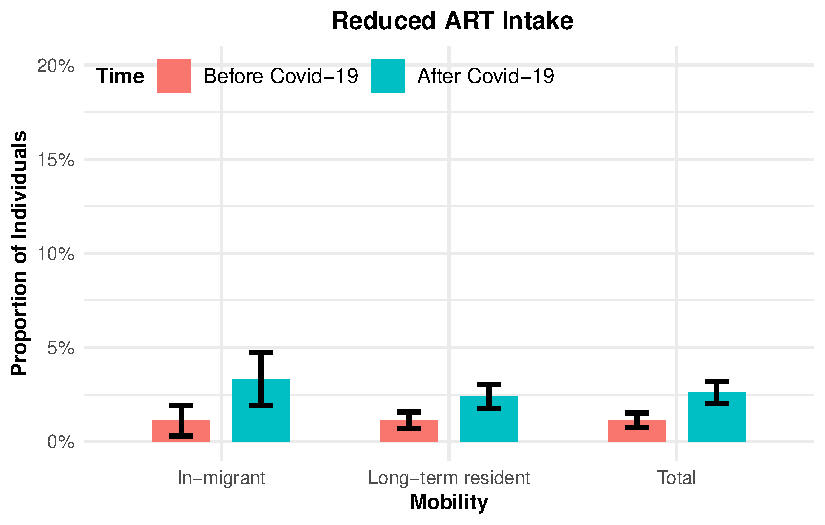
\includegraphics[keepaspectratio]{Rakai_revision_files/figure-pdf/unnamed-chunk-48-1.pdf}}

\subsubsection{Missed scheduled visits by
mobility}\label{missed-scheduled-visits-by-mobility}

\begin{Shaded}
\begin{Highlighting}[]
\NormalTok{df\_mob }\SpecialCharTok{\%\textgreater{}\%} \FunctionTok{group\_by}\NormalTok{(mobility,hivbc) }\SpecialCharTok{\%\textgreater{}\%} 
  \FunctionTok{count}\NormalTok{()}
\end{Highlighting}
\end{Shaded}

\begin{longtable}[]{@{}llr@{}}
\toprule\noalign{}
mobility & hivbc & n \\
\midrule\noalign{}
\endhead
\bottomrule\noalign{}
\endlastfoot
In-migrant & No & 595 \\
In-migrant & Yes & 37 \\
Long-term resident & No & 2144 \\
Long-term resident & Yes & 58 \\
\end{longtable}

\begin{Shaded}
\begin{Highlighting}[]
\NormalTok{df\_mob }\SpecialCharTok{\%\textgreater{}\%} \FunctionTok{group\_by}\NormalTok{(mobility,hivac) }\SpecialCharTok{\%\textgreater{}\%} 
  \FunctionTok{count}\NormalTok{()}
\end{Highlighting}
\end{Shaded}

\begin{longtable}[]{@{}llr@{}}
\toprule\noalign{}
mobility & hivac & n \\
\midrule\noalign{}
\endhead
\bottomrule\noalign{}
\endlastfoot
In-migrant & No & 534 \\
In-migrant & Yes & 98 \\
Long-term resident & No & 2025 \\
Long-term resident & Yes & 177 \\
\end{longtable}

\begin{Shaded}
\begin{Highlighting}[]
\NormalTok{df\_mob\_hiv }\OtherTok{\textless{}{-}}\NormalTok{ df\_mob }\SpecialCharTok{\%\textgreater{}\%}
  \FunctionTok{mutate}\NormalTok{(}
    \AttributeTok{hivbc =} \FunctionTok{as.character}\NormalTok{(hivbc),}
    \AttributeTok{hivac =} \FunctionTok{as.character}\NormalTok{(hivac)}
\NormalTok{  ) }\SpecialCharTok{\%\textgreater{}\%}
  \FunctionTok{pivot\_longer}\NormalTok{(}
    \AttributeTok{cols =} \FunctionTok{c}\NormalTok{(hivbc, hivac),}
    \AttributeTok{names\_to =} \StringTok{"variable"}\NormalTok{,}
    \AttributeTok{values\_to =} \StringTok{"response"}
\NormalTok{  ) }\SpecialCharTok{\%\textgreater{}\%}
  \FunctionTok{mutate}\NormalTok{(}
    \AttributeTok{time =} \FunctionTok{if\_else}\NormalTok{(}\FunctionTok{grepl}\NormalTok{(}\StringTok{"bc$"}\NormalTok{, variable), }\StringTok{"Before Covid{-}19"}\NormalTok{, }\StringTok{"After Covid{-}19"}\NormalTok{)}
\NormalTok{  )}

\NormalTok{df\_mob\_hiv\_summary }\OtherTok{\textless{}{-}}\NormalTok{ df\_mob\_hiv }\SpecialCharTok{\%\textgreater{}\%}
  \FunctionTok{group\_by}\NormalTok{(time,mobility) }\SpecialCharTok{\%\textgreater{}\%}
  \FunctionTok{summarise}\NormalTok{(}
    \AttributeTok{n\_yes =} \FunctionTok{sum}\NormalTok{(response }\SpecialCharTok{==} \StringTok{"Yes"}\NormalTok{, }\AttributeTok{na.rm =} \ConstantTok{TRUE}\NormalTok{),}
    \AttributeTok{n =} \FunctionTok{n}\NormalTok{(),}
    \AttributeTok{.groups =} \StringTok{"drop"}
\NormalTok{  )}

\NormalTok{df\_mob\_hiv\_totals }\OtherTok{\textless{}{-}}\NormalTok{ df\_mob\_hiv }\SpecialCharTok{\%\textgreater{}\%}
  \FunctionTok{group\_by}\NormalTok{(time) }\SpecialCharTok{\%\textgreater{}\%}
  \FunctionTok{summarise}\NormalTok{(}
    \AttributeTok{n\_yes =} \FunctionTok{sum}\NormalTok{(response }\SpecialCharTok{==} \StringTok{"Yes"}\NormalTok{, }\AttributeTok{na.rm =} \ConstantTok{TRUE}\NormalTok{),}
    \AttributeTok{n =} \FunctionTok{n}\NormalTok{(),}
    \AttributeTok{.groups =} \StringTok{"drop"}
\NormalTok{  ) }

\NormalTok{df\_mob\_hiv\_summary }\OtherTok{\textless{}{-}} \FunctionTok{bind\_rows}\NormalTok{(df\_mob\_hiv\_summary, df\_mob\_hiv\_totals) }\SpecialCharTok{\%\textgreater{}\%}
  \FunctionTok{mutate}\NormalTok{(}
    \AttributeTok{proportion =}\NormalTok{ n\_yes }\SpecialCharTok{/}\NormalTok{ n,}
    \AttributeTok{se =} \FunctionTok{sqrt}\NormalTok{(proportion }\SpecialCharTok{*}\NormalTok{ (}\DecValTok{1} \SpecialCharTok{{-}}\NormalTok{ proportion) }\SpecialCharTok{/}\NormalTok{ n),}
    \AttributeTok{lower =}\NormalTok{ proportion }\SpecialCharTok{{-}} \FloatTok{1.96} \SpecialCharTok{*}\NormalTok{ se,}
    \AttributeTok{upper =}\NormalTok{ proportion }\SpecialCharTok{+} \FloatTok{1.96} \SpecialCharTok{*}\NormalTok{ se}
\NormalTok{  )}\SpecialCharTok{\%\textgreater{}\%} 
  \FunctionTok{mutate}\NormalTok{(}\AttributeTok{time =} \FunctionTok{as\_factor}\NormalTok{(time) }\SpecialCharTok{\%\textgreater{}\%} 
           \FunctionTok{fct\_relevel}\NormalTok{(}\StringTok{"Before Covid{-}19"}\NormalTok{),}
         \AttributeTok{mobility =} \FunctionTok{if\_else}\NormalTok{(}\FunctionTok{is.na}\NormalTok{(mobility),}\StringTok{"Total"}\NormalTok{,mobility))}



\NormalTok{df\_com\_hiv\_summary}
\end{Highlighting}
\end{Shaded}

\begin{longtable}[]{@{}
  >{\raggedright\arraybackslash}p{(\linewidth - 14\tabcolsep) * \real{0.1860}}
  >{\raggedright\arraybackslash}p{(\linewidth - 14\tabcolsep) * \real{0.2093}}
  >{\raggedleft\arraybackslash}p{(\linewidth - 14\tabcolsep) * \real{0.0698}}
  >{\raggedleft\arraybackslash}p{(\linewidth - 14\tabcolsep) * \real{0.0581}}
  >{\raggedleft\arraybackslash}p{(\linewidth - 14\tabcolsep) * \real{0.1279}}
  >{\raggedleft\arraybackslash}p{(\linewidth - 14\tabcolsep) * \real{0.1163}}
  >{\raggedleft\arraybackslash}p{(\linewidth - 14\tabcolsep) * \real{0.1163}}
  >{\raggedleft\arraybackslash}p{(\linewidth - 14\tabcolsep) * \real{0.1163}}@{}}
\toprule\noalign{}
\begin{minipage}[b]{\linewidth}\raggedright
time
\end{minipage} & \begin{minipage}[b]{\linewidth}\raggedright
community\_type
\end{minipage} & \begin{minipage}[b]{\linewidth}\raggedleft
n\_yes
\end{minipage} & \begin{minipage}[b]{\linewidth}\raggedleft
n
\end{minipage} & \begin{minipage}[b]{\linewidth}\raggedleft
proportion
\end{minipage} & \begin{minipage}[b]{\linewidth}\raggedleft
se
\end{minipage} & \begin{minipage}[b]{\linewidth}\raggedleft
lower
\end{minipage} & \begin{minipage}[b]{\linewidth}\raggedleft
upper
\end{minipage} \\
\midrule\noalign{}
\endhead
\bottomrule\noalign{}
\endlastfoot
After Covid-19 & Inland Community & 85 & 1283 & 0.0662510 & 0.0069438 &
0.0526411 & 0.0798608 \\
After Covid-19 & Fishing community & 190 & 1551 & 0.1225016 & 0.0083251
& 0.1061845 & 0.1388188 \\
Before Covid-19 & Inland Community & 26 & 1283 & 0.0202650 & 0.0039338 &
0.0125547 & 0.0279753 \\
Before Covid-19 & Fishing community & 69 & 1551 & 0.0444874 & 0.0052352
& 0.0342265 & 0.0547484 \\
After Covid-19 & Total & 275 & 2834 & 0.0970360 & 0.0055603 & 0.0861377
& 0.1079343 \\
Before Covid-19 & Total & 95 & 2834 & 0.0335215 & 0.0033811 & 0.0268946
& 0.0401485 \\
\end{longtable}

\begin{Shaded}
\begin{Highlighting}[]
\NormalTok{missed\_scheduled\_visit\_by\_mobility\_plot }\OtherTok{\textless{}{-}}  \FunctionTok{ggplot}\NormalTok{(df\_mob\_hiv\_summary, }\FunctionTok{aes}\NormalTok{(}\AttributeTok{x =}\NormalTok{ mobility, }\AttributeTok{y =}\NormalTok{ proportion, }\AttributeTok{fill =}\NormalTok{ time)) }\SpecialCharTok{+}
  \FunctionTok{geom\_col}\NormalTok{(}\AttributeTok{position =} \FunctionTok{position\_dodge}\NormalTok{(}\AttributeTok{width =} \FloatTok{0.7}\NormalTok{), }\AttributeTok{width =} \FloatTok{0.5}\NormalTok{) }\SpecialCharTok{+}
  \FunctionTok{geom\_errorbar}\NormalTok{(}
    \FunctionTok{aes}\NormalTok{(}\AttributeTok{ymin =}\NormalTok{ lower, }\AttributeTok{ymax =}\NormalTok{ upper),}
    \AttributeTok{position =} \FunctionTok{position\_dodge}\NormalTok{(}\AttributeTok{width =} \FloatTok{0.7}\NormalTok{),}
    \AttributeTok{width =} \FloatTok{0.2}\NormalTok{,}
    \AttributeTok{size =} \DecValTok{1}
\NormalTok{  ) }\SpecialCharTok{+}
  \FunctionTok{scale\_y\_continuous}\NormalTok{(}\AttributeTok{labels =}\NormalTok{ scales}\SpecialCharTok{::}\FunctionTok{percent\_format}\NormalTok{(}\AttributeTok{accuracy =} \DecValTok{1}\NormalTok{),}\AttributeTok{limits =} \FunctionTok{c}\NormalTok{(}\DecValTok{0}\NormalTok{, }\FloatTok{0.2}\NormalTok{)) }\SpecialCharTok{+}
  \FunctionTok{labs}\NormalTok{(}
    \AttributeTok{title =} \StringTok{"Missed Scheduled Visits"}\NormalTok{,}
    \AttributeTok{x =} \StringTok{"Mobility"}\NormalTok{,}
    \AttributeTok{y =} \StringTok{"Proportion of individuals"}\NormalTok{,}
    \AttributeTok{fill =} \StringTok{"Time"}
\NormalTok{  ) }\SpecialCharTok{+}
  \FunctionTok{theme\_minimal}\NormalTok{() }\SpecialCharTok{+}
  \FunctionTok{theme}\NormalTok{(}
    \AttributeTok{plot.title =} \FunctionTok{element\_text}\NormalTok{(}\AttributeTok{hjust =} \FloatTok{0.5}\NormalTok{, }\AttributeTok{face =} \StringTok{"bold"}\NormalTok{, }\AttributeTok{size =} \DecValTok{12}\NormalTok{),}
    \AttributeTok{axis.title.x =} \FunctionTok{element\_text}\NormalTok{(}\AttributeTok{face =} \StringTok{"bold"}\NormalTok{, }\AttributeTok{size =} \DecValTok{10}\NormalTok{),}
    \AttributeTok{axis.title.y =} \FunctionTok{element\_text}\NormalTok{(}\AttributeTok{face =} \StringTok{"bold"}\NormalTok{, }\AttributeTok{size =} \DecValTok{10}\NormalTok{),}
    \AttributeTok{legend.title =} \FunctionTok{element\_text}\NormalTok{(}\AttributeTok{face =} \StringTok{"bold"}\NormalTok{, }\AttributeTok{size =} \DecValTok{10}\NormalTok{),}
    \AttributeTok{legend.text =} \FunctionTok{element\_text}\NormalTok{(}\AttributeTok{size =} \DecValTok{10}\NormalTok{),}
    \AttributeTok{legend.position =} \FunctionTok{c}\NormalTok{(}\DecValTok{0}\NormalTok{, }\DecValTok{1}\NormalTok{),}
    \AttributeTok{legend.justification =} \FunctionTok{c}\NormalTok{(}\DecValTok{0}\NormalTok{, }\DecValTok{1}\NormalTok{),}
    \AttributeTok{legend.direction =} \StringTok{"horizontal"}
\NormalTok{  )}

\NormalTok{missed\_scheduled\_visit\_by\_mobility\_plot}
\end{Highlighting}
\end{Shaded}

\pandocbounded{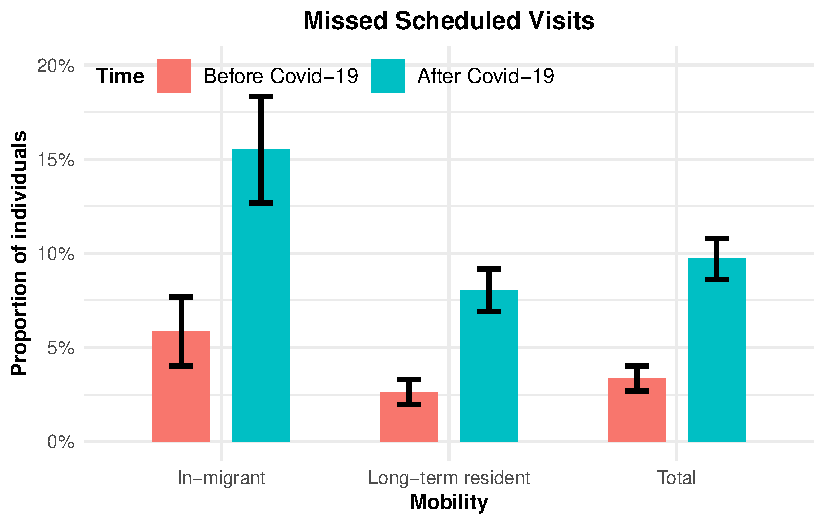
\includegraphics[keepaspectratio]{Rakai_revision_files/figure-pdf/unnamed-chunk-51-1.pdf}}

\begin{Shaded}
\begin{Highlighting}[]
\NormalTok{pm1 }\OtherTok{\textless{}{-}} \FunctionTok{ggplot}\NormalTok{(df\_mob\_artstr\_summary, }\FunctionTok{aes}\NormalTok{(}\AttributeTok{x =}\NormalTok{ mobility, }\AttributeTok{y =}\NormalTok{ proportion, }\AttributeTok{fill =}\NormalTok{time)) }\SpecialCharTok{+}
  \FunctionTok{geom\_col}\NormalTok{(}\AttributeTok{position =} \FunctionTok{position\_dodge}\NormalTok{(}\AttributeTok{width =} \FloatTok{0.7}\NormalTok{), }\AttributeTok{width =} \FloatTok{0.5}\NormalTok{) }\SpecialCharTok{+}
  \FunctionTok{geom\_errorbar}\NormalTok{(}
    \FunctionTok{aes}\NormalTok{(}\AttributeTok{ymin =}\NormalTok{ lower, }\AttributeTok{ymax =}\NormalTok{ upper),}
    \AttributeTok{position =} \FunctionTok{position\_dodge}\NormalTok{(}\AttributeTok{width =} \FloatTok{0.7}\NormalTok{),}
    \AttributeTok{width =} \FloatTok{0.2}\NormalTok{,}
    \AttributeTok{size =} \DecValTok{1}
\NormalTok{  ) }\SpecialCharTok{+}
  \FunctionTok{scale\_y\_continuous}\NormalTok{(}\AttributeTok{labels =}\NormalTok{ scales}\SpecialCharTok{::}\FunctionTok{percent\_format}\NormalTok{(}\AttributeTok{accuracy =} \DecValTok{1}\NormalTok{),}\AttributeTok{limits =} \FunctionTok{c}\NormalTok{(}\DecValTok{0}\NormalTok{, }\FloatTok{0.25}\NormalTok{)) }\SpecialCharTok{+}
  \FunctionTok{labs}\NormalTok{(}
    \AttributeTok{title =} \StringTok{"Reduced ART Intake"}\NormalTok{,}
    \AttributeTok{x =} \StringTok{"Mobility"}\NormalTok{,}
    \AttributeTok{y =} \StringTok{"Proportion of individuals"}\NormalTok{,}
    \AttributeTok{fill =} \StringTok{"Time"}
\NormalTok{  ) }\SpecialCharTok{+}
  \FunctionTok{theme\_minimal}\NormalTok{() }\SpecialCharTok{+}
  \FunctionTok{theme}\NormalTok{(}
    \AttributeTok{plot.title =} \FunctionTok{element\_text}\NormalTok{(}\AttributeTok{hjust =} \FloatTok{0.5}\NormalTok{, }\AttributeTok{face =} \StringTok{"bold"}\NormalTok{, }\AttributeTok{size =} \DecValTok{12}\NormalTok{),}
    \AttributeTok{axis.title.x =} \FunctionTok{element\_text}\NormalTok{(}\AttributeTok{face =} \StringTok{"bold"}\NormalTok{, }\AttributeTok{size =} \DecValTok{10}\NormalTok{),}
    \AttributeTok{axis.title.y =} \FunctionTok{element\_text}\NormalTok{(}\AttributeTok{face =} \StringTok{"bold"}\NormalTok{, }\AttributeTok{size =} \DecValTok{10}\NormalTok{),}
    \AttributeTok{legend.title =} \FunctionTok{element\_text}\NormalTok{(}\AttributeTok{face =} \StringTok{"bold"}\NormalTok{, }\AttributeTok{size =} \DecValTok{10}\NormalTok{),}
    \AttributeTok{legend.text =} \FunctionTok{element\_text}\NormalTok{(}\AttributeTok{size =} \DecValTok{10}\NormalTok{),}
    \AttributeTok{legend.position =} \FunctionTok{c}\NormalTok{(}\DecValTok{0}\NormalTok{, }\DecValTok{1}\NormalTok{),}
    \AttributeTok{legend.justification =} \FunctionTok{c}\NormalTok{(}\DecValTok{0}\NormalTok{, }\DecValTok{1}\NormalTok{),}
    \AttributeTok{legend.direction =} \StringTok{"horizontal"}
\NormalTok{  )}
\NormalTok{pm1 }\DocumentationTok{\#\#}
\end{Highlighting}
\end{Shaded}

\pandocbounded{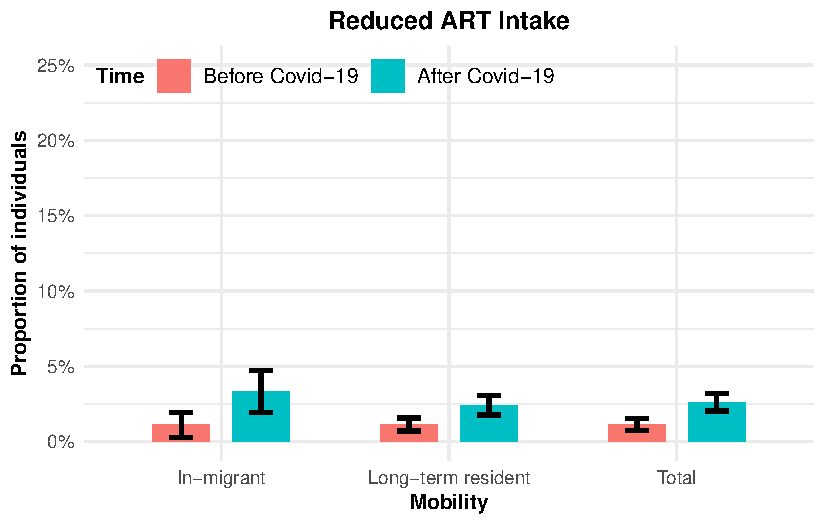
\includegraphics[keepaspectratio]{Rakai_revision_files/figure-pdf/unnamed-chunk-52-1.pdf}}

\begin{Shaded}
\begin{Highlighting}[]
\NormalTok{pm2 }\OtherTok{\textless{}{-}} \FunctionTok{ggplot}\NormalTok{(df\_mob\_hiv\_summary, }\FunctionTok{aes}\NormalTok{(}\AttributeTok{x =}\NormalTok{ mobility, }\AttributeTok{y =}\NormalTok{ proportion, }\AttributeTok{fill =}\NormalTok{ time)) }\SpecialCharTok{+}
  \FunctionTok{geom\_col}\NormalTok{(}\AttributeTok{position =} \FunctionTok{position\_dodge}\NormalTok{(}\AttributeTok{width =} \FloatTok{0.7}\NormalTok{), }\AttributeTok{width =} \FloatTok{0.5}\NormalTok{) }\SpecialCharTok{+}
  \FunctionTok{geom\_errorbar}\NormalTok{(}
    \FunctionTok{aes}\NormalTok{(}\AttributeTok{ymin =}\NormalTok{ lower, }\AttributeTok{ymax =}\NormalTok{ upper),}
    \AttributeTok{position =} \FunctionTok{position\_dodge}\NormalTok{(}\AttributeTok{width =} \FloatTok{0.7}\NormalTok{),}
    \AttributeTok{width =} \FloatTok{0.2}\NormalTok{,}
    \AttributeTok{size =} \DecValTok{1}
\NormalTok{  ) }\SpecialCharTok{+}
  \FunctionTok{scale\_y\_continuous}\NormalTok{(}\AttributeTok{labels =}\NormalTok{ scales}\SpecialCharTok{::}\FunctionTok{percent\_format}\NormalTok{(}\AttributeTok{accuracy =} \DecValTok{1}\NormalTok{),}\AttributeTok{limits =} \FunctionTok{c}\NormalTok{(}\DecValTok{0}\NormalTok{, }\FloatTok{0.25}\NormalTok{)) }\SpecialCharTok{+}
  \FunctionTok{labs}\NormalTok{(}
    \AttributeTok{caption =} \StringTok{"Missed Scheduled Visits"}\NormalTok{,}
    \AttributeTok{x =} \StringTok{"Mobility"}\NormalTok{,}
    \AttributeTok{y =} \StringTok{"Proportion of individuals"}\NormalTok{,}
    \AttributeTok{fill =} \StringTok{"Time"}
\NormalTok{  ) }\SpecialCharTok{+}
  \FunctionTok{theme\_minimal}\NormalTok{() }\SpecialCharTok{+}
  \FunctionTok{theme}\NormalTok{(}
    \AttributeTok{plot.caption =} \FunctionTok{element\_text}\NormalTok{(}\AttributeTok{hjust =} \DecValTok{0}\NormalTok{, }\AttributeTok{face =} \StringTok{"bold"}\NormalTok{, }\AttributeTok{size =} \DecValTok{10}\NormalTok{),}
    \AttributeTok{axis.title.x =} \FunctionTok{element\_text}\NormalTok{(}\AttributeTok{face =} \StringTok{"bold"}\NormalTok{, }\AttributeTok{size =} \DecValTok{10}\NormalTok{),}
    \AttributeTok{axis.title.y =} \FunctionTok{element\_text}\NormalTok{(}\AttributeTok{face =} \StringTok{"bold"}\NormalTok{, }\AttributeTok{size =} \DecValTok{10}\NormalTok{),}
    \AttributeTok{legend.title =} \FunctionTok{element\_text}\NormalTok{(}\AttributeTok{face =} \StringTok{"bold"}\NormalTok{, }\AttributeTok{size =} \DecValTok{10}\NormalTok{),}
    \AttributeTok{legend.text =} \FunctionTok{element\_text}\NormalTok{(}\AttributeTok{size =} \DecValTok{10}\NormalTok{),}
    \AttributeTok{legend.position =} \FunctionTok{c}\NormalTok{(}\DecValTok{0}\NormalTok{, }\DecValTok{1}\NormalTok{),}
    \AttributeTok{legend.justification =} \FunctionTok{c}\NormalTok{(}\DecValTok{0}\NormalTok{, }\DecValTok{1}\NormalTok{),}
    \AttributeTok{legend.direction =} \StringTok{"horizontal"}
\NormalTok{  )}
\NormalTok{pm2 }\DocumentationTok{\#\# Missed scheduled vis}
\end{Highlighting}
\end{Shaded}

\pandocbounded{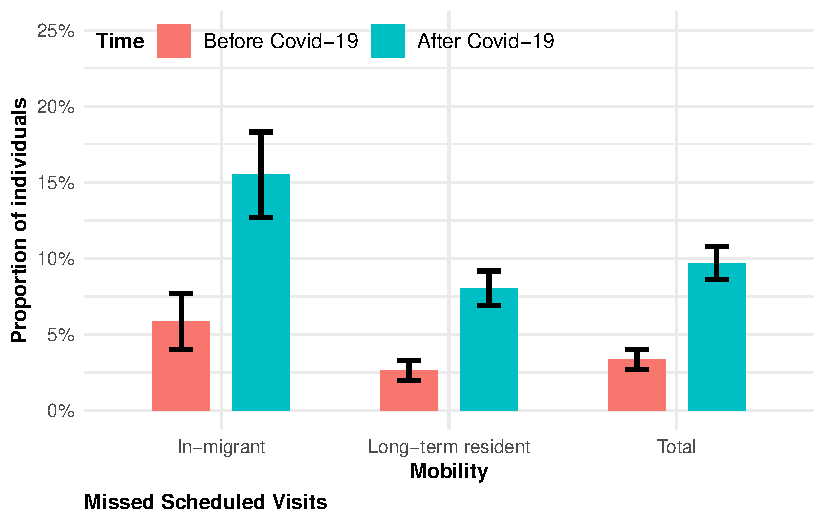
\includegraphics[keepaspectratio]{Rakai_revision_files/figure-pdf/unnamed-chunk-53-1.pdf}}

\begin{Shaded}
\begin{Highlighting}[]
\NormalTok{pm3 }\OtherTok{\textless{}{-}} \FunctionTok{ggplot}\NormalTok{(df\_mob\_artrun\_summary, }\FunctionTok{aes}\NormalTok{(}\AttributeTok{x =}\NormalTok{ mobility, }\AttributeTok{y =}\NormalTok{ proportion, }\AttributeTok{fill =}\NormalTok{time)) }\SpecialCharTok{+}
  \FunctionTok{geom\_col}\NormalTok{(}\AttributeTok{position =} \FunctionTok{position\_dodge}\NormalTok{(}\AttributeTok{width =} \FloatTok{0.7}\NormalTok{), }\AttributeTok{width =} \FloatTok{0.5}\NormalTok{) }\SpecialCharTok{+}
  \FunctionTok{geom\_errorbar}\NormalTok{(}
    \FunctionTok{aes}\NormalTok{(}\AttributeTok{ymin =}\NormalTok{ lower, }\AttributeTok{ymax =}\NormalTok{ upper),}
    \AttributeTok{position =} \FunctionTok{position\_dodge}\NormalTok{(}\AttributeTok{width =} \FloatTok{0.7}\NormalTok{),}
    \AttributeTok{width =} \FloatTok{0.2}\NormalTok{,}
    \AttributeTok{size =} \DecValTok{1}
\NormalTok{  ) }\SpecialCharTok{+}
  \FunctionTok{scale\_y\_continuous}\NormalTok{(}\AttributeTok{labels =}\NormalTok{ scales}\SpecialCharTok{::}\FunctionTok{percent\_format}\NormalTok{(}\AttributeTok{accuracy =} \DecValTok{1}\NormalTok{),}\AttributeTok{limits =} \FunctionTok{c}\NormalTok{(}\DecValTok{0}\NormalTok{, }\FloatTok{0.25}\NormalTok{)) }\SpecialCharTok{+}
  \FunctionTok{labs}\NormalTok{(}
    \AttributeTok{title =}  \StringTok{"Run Out of ART"}\NormalTok{,}
    \AttributeTok{x =} \StringTok{"Mobility"}\NormalTok{,}
    \AttributeTok{y =} \StringTok{"Proportion of individuals"}\NormalTok{,}
    \AttributeTok{fill =} \StringTok{"Time"}
\NormalTok{  ) }\SpecialCharTok{+}
  \FunctionTok{theme\_minimal}\NormalTok{() }\SpecialCharTok{+}
  \FunctionTok{theme}\NormalTok{(}
    \AttributeTok{plot.title =}  \FunctionTok{element\_text}\NormalTok{(}\AttributeTok{hjust =} \FloatTok{0.5}\NormalTok{, }\AttributeTok{face =} \StringTok{"bold"}\NormalTok{, }\AttributeTok{size =} \DecValTok{12}\NormalTok{),}
    \AttributeTok{axis.title.x =} \FunctionTok{element\_text}\NormalTok{(}\AttributeTok{face =} \StringTok{"bold"}\NormalTok{, }\AttributeTok{size =} \DecValTok{10}\NormalTok{),}
    \AttributeTok{axis.title.y =} \FunctionTok{element\_text}\NormalTok{(}\AttributeTok{face =} \StringTok{"bold"}\NormalTok{, }\AttributeTok{size =} \DecValTok{10}\NormalTok{),}
    \AttributeTok{legend.title =} \FunctionTok{element\_text}\NormalTok{(}\AttributeTok{face =} \StringTok{"bold"}\NormalTok{, }\AttributeTok{size =} \DecValTok{10}\NormalTok{),}
    \AttributeTok{legend.text =} \FunctionTok{element\_text}\NormalTok{(}\AttributeTok{size =} \DecValTok{10}\NormalTok{),}
    \AttributeTok{legend.position =} \FunctionTok{c}\NormalTok{(}\DecValTok{0}\NormalTok{, }\DecValTok{1}\NormalTok{),}
    \AttributeTok{legend.justification =} \FunctionTok{c}\NormalTok{(}\DecValTok{0}\NormalTok{, }\DecValTok{1}\NormalTok{),}
    \AttributeTok{legend.direction =} \StringTok{"horizontal"}
\NormalTok{  )}

\NormalTok{pm3}
\end{Highlighting}
\end{Shaded}

\pandocbounded{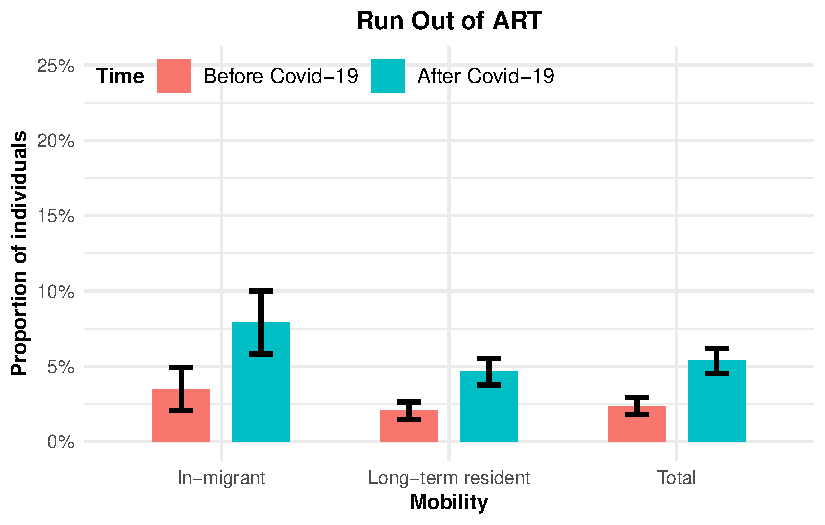
\includegraphics[keepaspectratio]{Rakai_revision_files/figure-pdf/unnamed-chunk-54-1.pdf}}

\begin{Shaded}
\begin{Highlighting}[]
\DocumentationTok{\#\#\# Combined plot}
\NormalTok{(pm1 }\SpecialCharTok{+}\NormalTok{ pm2)}\SpecialCharTok{/}\NormalTok{pm3}
\end{Highlighting}
\end{Shaded}

\pandocbounded{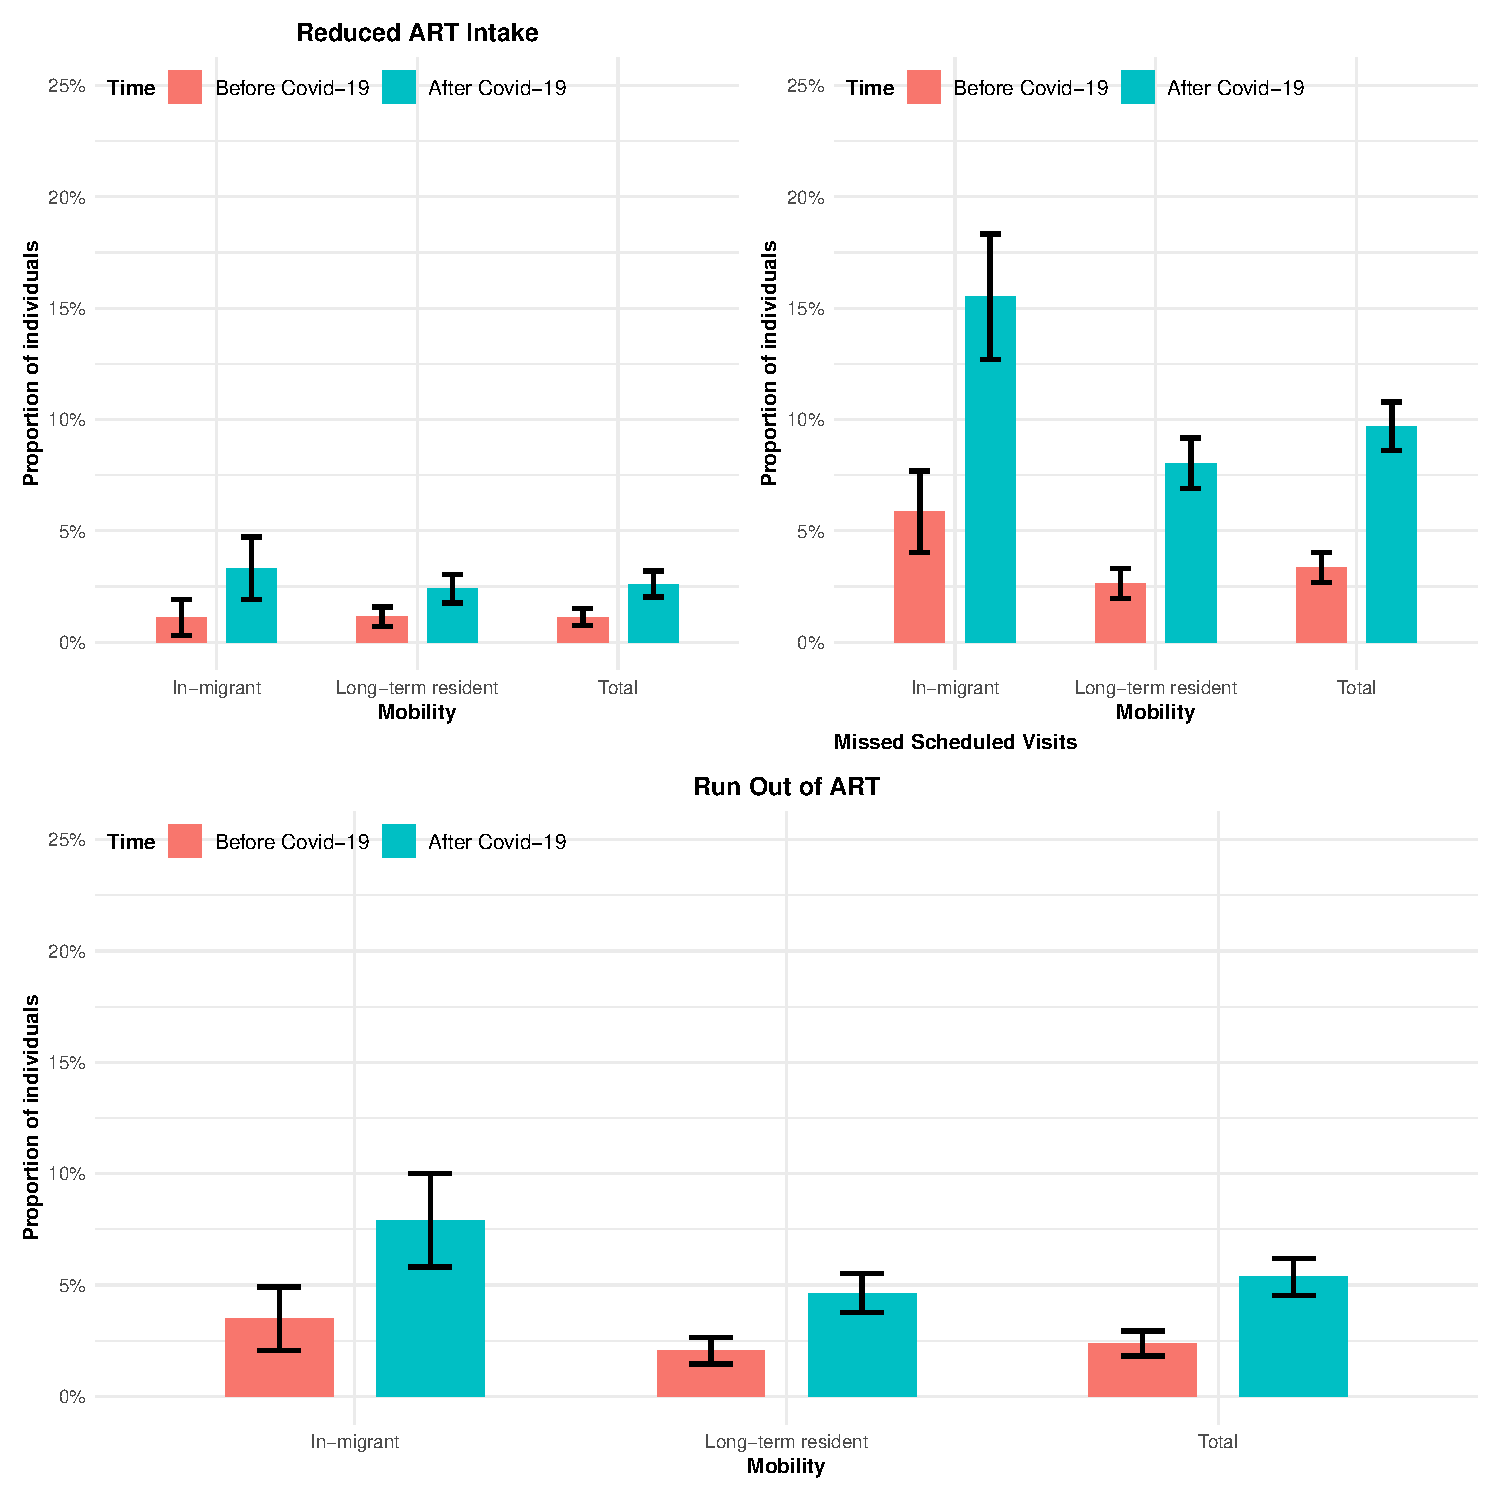
\includegraphics[keepaspectratio]{Rakai_revision_files/figure-pdf/unnamed-chunk-55-1.pdf}}

\subsubsection{Age Categories}\label{age-categories}

\begin{Shaded}
\begin{Highlighting}[]
\NormalTok{df\_age }\OtherTok{\textless{}{-}}\NormalTok{  rakai }\SpecialCharTok{\%\textgreater{}\%} 
  \FunctionTok{select}\NormalTok{(ageyrs,artrunbc,artrunac,}
\NormalTok{         hivac,hivbc,copies,new\_copies,artstrac,artstrbc) }\SpecialCharTok{\%\textgreater{}\%} 
  \FunctionTok{filter}\NormalTok{(hivac }\SpecialCharTok{!=}\DecValTok{8}\NormalTok{, hivbc}\SpecialCharTok{!=}\DecValTok{8}\NormalTok{,artrunbc}\SpecialCharTok{!=}\DecValTok{8}\NormalTok{,artstrac}\SpecialCharTok{!=}\DecValTok{8}\NormalTok{,artstrbc}\SpecialCharTok{!=}\DecValTok{8}\NormalTok{,artrunac}\SpecialCharTok{!=}\DecValTok{8}\NormalTok{) }\SpecialCharTok{\%\textgreater{}\%} 
  \FunctionTok{mutate}\NormalTok{(}
     \AttributeTok{age\_cat =} \FunctionTok{case\_when}\NormalTok{(}
\NormalTok{                             ageyrs }\SpecialCharTok{\textless{}} \DecValTok{30} \SpecialCharTok{\textasciitilde{}} \StringTok{"\textless{}30"}\NormalTok{,}
\NormalTok{                             ageyrs }\SpecialCharTok{\textgreater{}=} \DecValTok{30} \SpecialCharTok{\&}\NormalTok{ ageyrs }\SpecialCharTok{\textless{}=} \DecValTok{39} \SpecialCharTok{\textasciitilde{}}  \StringTok{"30{-}39"}\NormalTok{,}
\NormalTok{                             ageyrs }\SpecialCharTok{\textgreater{}=}\DecValTok{40} \SpecialCharTok{\&}\NormalTok{ ageyrs }\SpecialCharTok{\textless{}=} \DecValTok{49} \SpecialCharTok{\textasciitilde{}} \StringTok{"40{-}49"}\NormalTok{) }\SpecialCharTok{\%\textgreater{}\%} 
           \FunctionTok{fct\_relevel}\NormalTok{(}\StringTok{"\textless{}30"}\NormalTok{) }\SpecialCharTok{\%\textgreater{}\%} 
           \FunctionTok{ff\_label}\NormalTok{(}\StringTok{"Age group"}\NormalTok{),}
  
    \AttributeTok{hivac =} \FunctionTok{if\_else}\NormalTok{(hivac }\SpecialCharTok{==}\DecValTok{1}\NormalTok{, }\StringTok{"Yes"}\NormalTok{,}\StringTok{"No"}\NormalTok{) }\SpecialCharTok{\%\textgreater{}\%} 
    \FunctionTok{ff\_label}\NormalTok{(}\StringTok{"Missed scheduled visit for HIV care"}\NormalTok{) }\SpecialCharTok{\%\textgreater{}\%} 
      \FunctionTok{as\_factor}\NormalTok{(),}
   
     \AttributeTok{hivbc =} \FunctionTok{if\_else}\NormalTok{(hivbc }\SpecialCharTok{==}\DecValTok{1}\NormalTok{,}\StringTok{"Yes"}\NormalTok{,}\StringTok{"No"}\NormalTok{) }\SpecialCharTok{\%\textgreater{}\%} 
    \FunctionTok{ff\_label}\NormalTok{(}\StringTok{"Missed scheduled visit for HIV care"}\NormalTok{) }\SpecialCharTok{\%\textgreater{}\%} 
    \FunctionTok{as\_factor}\NormalTok{(),}
 
     \AttributeTok{artrunac =} \FunctionTok{if\_else}\NormalTok{(artrunac }\SpecialCharTok{==}\DecValTok{1}\NormalTok{,}\StringTok{"Yes"}\NormalTok{,}\StringTok{"No"}\NormalTok{) }\SpecialCharTok{\%\textgreater{}\%} 
    \FunctionTok{as\_factor}\NormalTok{() }\SpecialCharTok{\%\textgreater{}\%} 
    \FunctionTok{ff\_label}\NormalTok{(}\StringTok{"Run out of ART before next refill"}\NormalTok{),}
 
   \AttributeTok{artrunbc =} \FunctionTok{if\_else}\NormalTok{(artrunbc }\SpecialCharTok{==}\DecValTok{1}\NormalTok{,}\StringTok{"Yes"}\NormalTok{,}\StringTok{"No"}\NormalTok{) }\SpecialCharTok{\%\textgreater{}\%} 
    \FunctionTok{as\_factor}\NormalTok{() }\SpecialCharTok{\%\textgreater{}\%} 
    \FunctionTok{ff\_label}\NormalTok{(}\StringTok{"Run out of ART before next refill"}\NormalTok{),}
  
  \AttributeTok{artstrac =} \FunctionTok{if\_else}\NormalTok{(artstrac }\SpecialCharTok{==}\DecValTok{1}\NormalTok{,}\StringTok{"Yes"}\NormalTok{,}\StringTok{"No"}\NormalTok{) }\SpecialCharTok{\%\textgreater{}\%} 
    \FunctionTok{as\_factor}\NormalTok{() }\SpecialCharTok{\%\textgreater{}\%} 
    \FunctionTok{ff\_label}\NormalTok{(}\StringTok{"Taken ART pills less frequently / in smaller}
\StringTok{amounts to conserve supply"}\NormalTok{),}
  
  \AttributeTok{artstrbc =} \FunctionTok{if\_else}\NormalTok{(artstrbc }\SpecialCharTok{==}\DecValTok{1}\NormalTok{,}\StringTok{"Yes"}\NormalTok{,}\StringTok{"No"}\NormalTok{) }\SpecialCharTok{\%\textgreater{}\%} 
    \FunctionTok{as\_factor}\NormalTok{() }\SpecialCharTok{\%\textgreater{}\%} 
    \FunctionTok{ff\_label}\NormalTok{(}\StringTok{"Taken ART pills less frequently / in smaller}
\StringTok{amounts to conserve supply"}\NormalTok{)}
\NormalTok{  ) }\SpecialCharTok{\%\textgreater{}\%} 
  \FunctionTok{select}\NormalTok{(}\SpecialCharTok{{-}}\NormalTok{ageyrs)}
\end{Highlighting}
\end{Shaded}

\begin{Shaded}
\begin{Highlighting}[]
\CommentTok{\# df\_age}
\end{Highlighting}
\end{Shaded}

\subsubsection{Run out of ART by Age
Category}\label{run-out-of-art-by-age-category}

\begin{Shaded}
\begin{Highlighting}[]
\NormalTok{df\_age }\SpecialCharTok{\%\textgreater{}\%} \FunctionTok{group\_by}\NormalTok{(age\_cat,artrunbc) }\SpecialCharTok{\%\textgreater{}\%} 
  \FunctionTok{count}\NormalTok{()}
\end{Highlighting}
\end{Shaded}

\begin{longtable}[]{@{}llr@{}}
\toprule\noalign{}
age\_cat & artrunbc & n \\
\midrule\noalign{}
\endhead
\bottomrule\noalign{}
\endlastfoot
\textless30 & No & 421 \\
\textless30 & Yes & 12 \\
30-39 & No & 1198 \\
30-39 & Yes & 31 \\
40-49 & No & 1148 \\
40-49 & Yes & 24 \\
\end{longtable}

\begin{Shaded}
\begin{Highlighting}[]
\NormalTok{df\_age }\SpecialCharTok{\%\textgreater{}\%} \FunctionTok{group\_by}\NormalTok{(age\_cat,artrunac) }\SpecialCharTok{\%\textgreater{}\%} 
  \FunctionTok{count}\NormalTok{()}
\end{Highlighting}
\end{Shaded}

\begin{longtable}[]{@{}llr@{}}
\toprule\noalign{}
age\_cat & artrunac & n \\
\midrule\noalign{}
\endhead
\bottomrule\noalign{}
\endlastfoot
\textless30 & No & 401 \\
\textless30 & Yes & 32 \\
30-39 & No & 1158 \\
30-39 & Yes & 71 \\
40-49 & No & 1123 \\
40-49 & Yes & 49 \\
\end{longtable}

\begin{Shaded}
\begin{Highlighting}[]
\NormalTok{df\_age\_artrun }\OtherTok{\textless{}{-}}\NormalTok{ df\_age }\SpecialCharTok{\%\textgreater{}\%}
  \FunctionTok{mutate}\NormalTok{(}
    \AttributeTok{artrunbc =} \FunctionTok{as.character}\NormalTok{(artrunbc),}
    \AttributeTok{artrunac =} \FunctionTok{as.character}\NormalTok{(artrunac)}
\NormalTok{  ) }\SpecialCharTok{\%\textgreater{}\%}
  \FunctionTok{pivot\_longer}\NormalTok{(}
    \AttributeTok{cols =} \FunctionTok{c}\NormalTok{(artrunbc, artrunac),}
    \AttributeTok{names\_to =} \StringTok{"variable"}\NormalTok{,}
    \AttributeTok{values\_to =} \StringTok{"response"}
\NormalTok{  ) }\SpecialCharTok{\%\textgreater{}\%}
  \FunctionTok{mutate}\NormalTok{(}
    \AttributeTok{time =} \FunctionTok{if\_else}\NormalTok{(}\FunctionTok{grepl}\NormalTok{(}\StringTok{"bc$"}\NormalTok{, variable), }\StringTok{"Before Covid{-}19"}\NormalTok{, }\StringTok{"After Covid{-}19"}\NormalTok{)}
\NormalTok{  )}

\NormalTok{df\_age\_artrun\_summary }\OtherTok{\textless{}{-}}\NormalTok{ df\_age\_artrun }\SpecialCharTok{\%\textgreater{}\%}
  \FunctionTok{group\_by}\NormalTok{(time, age\_cat) }\SpecialCharTok{\%\textgreater{}\%}
  \FunctionTok{summarise}\NormalTok{(}
    \AttributeTok{n\_yes =} \FunctionTok{sum}\NormalTok{(response }\SpecialCharTok{==} \StringTok{"Yes"}\NormalTok{, }\AttributeTok{na.rm =} \ConstantTok{TRUE}\NormalTok{),}
    \AttributeTok{n =} \FunctionTok{n}\NormalTok{(),}
    \AttributeTok{.groups =} \StringTok{"drop"}
\NormalTok{  )}

\NormalTok{df\_age\_artrun\_totals }\OtherTok{\textless{}{-}}\NormalTok{ df\_age\_artrun }\SpecialCharTok{\%\textgreater{}\%}
  \FunctionTok{group\_by}\NormalTok{(time) }\SpecialCharTok{\%\textgreater{}\%}
  \FunctionTok{summarise}\NormalTok{(}
    \AttributeTok{n\_yes =} \FunctionTok{sum}\NormalTok{(response }\SpecialCharTok{==} \StringTok{"Yes"}\NormalTok{, }\AttributeTok{na.rm =} \ConstantTok{TRUE}\NormalTok{),}
    \AttributeTok{n =} \FunctionTok{n}\NormalTok{(),}
    \AttributeTok{.groups =} \StringTok{"drop"}
\NormalTok{  )}

\NormalTok{df\_age\_artrun\_summary }\OtherTok{\textless{}{-}} \FunctionTok{bind\_rows}\NormalTok{(df\_age\_artrun\_summary, df\_age\_artrun\_totals) }\SpecialCharTok{\%\textgreater{}\%}
  \FunctionTok{mutate}\NormalTok{(}
    \AttributeTok{proportion =}\NormalTok{ n\_yes }\SpecialCharTok{/}\NormalTok{ n,}
    \AttributeTok{se =} \FunctionTok{sqrt}\NormalTok{(proportion }\SpecialCharTok{*}\NormalTok{ (}\DecValTok{1} \SpecialCharTok{{-}}\NormalTok{ proportion) }\SpecialCharTok{/}\NormalTok{ n),}
    \AttributeTok{lower =}\NormalTok{ proportion }\SpecialCharTok{{-}} \FloatTok{1.96} \SpecialCharTok{*}\NormalTok{ se,}
    \AttributeTok{upper =}\NormalTok{ proportion }\SpecialCharTok{+} \FloatTok{1.96} \SpecialCharTok{*}\NormalTok{ se}
\NormalTok{  ) }\SpecialCharTok{\%\textgreater{}\%} 
  \FunctionTok{mutate}\NormalTok{(}
    \AttributeTok{time =} \FunctionTok{as\_factor}\NormalTok{(time) }\SpecialCharTok{\%\textgreater{}\%} 
      \FunctionTok{fct\_relevel}\NormalTok{(}\StringTok{"Before Covid{-}19"}\NormalTok{),}
    \AttributeTok{age\_cat =} \FunctionTok{if\_else}\NormalTok{(}\FunctionTok{is.na}\NormalTok{(age\_cat), }\StringTok{"Total"}\NormalTok{, age\_cat)}
\NormalTok{  )}

\NormalTok{df\_age\_artrun\_summary}
\end{Highlighting}
\end{Shaded}

\begin{longtable}[]{@{}
  >{\raggedright\arraybackslash}p{(\linewidth - 14\tabcolsep) * \real{0.2105}}
  >{\raggedright\arraybackslash}p{(\linewidth - 14\tabcolsep) * \real{0.1053}}
  >{\raggedleft\arraybackslash}p{(\linewidth - 14\tabcolsep) * \real{0.0789}}
  >{\raggedleft\arraybackslash}p{(\linewidth - 14\tabcolsep) * \real{0.0658}}
  >{\raggedleft\arraybackslash}p{(\linewidth - 14\tabcolsep) * \real{0.1447}}
  >{\raggedleft\arraybackslash}p{(\linewidth - 14\tabcolsep) * \real{0.1316}}
  >{\raggedleft\arraybackslash}p{(\linewidth - 14\tabcolsep) * \real{0.1316}}
  >{\raggedleft\arraybackslash}p{(\linewidth - 14\tabcolsep) * \real{0.1316}}@{}}
\toprule\noalign{}
\begin{minipage}[b]{\linewidth}\raggedright
time
\end{minipage} & \begin{minipage}[b]{\linewidth}\raggedright
age\_cat
\end{minipage} & \begin{minipage}[b]{\linewidth}\raggedleft
n\_yes
\end{minipage} & \begin{minipage}[b]{\linewidth}\raggedleft
n
\end{minipage} & \begin{minipage}[b]{\linewidth}\raggedleft
proportion
\end{minipage} & \begin{minipage}[b]{\linewidth}\raggedleft
se
\end{minipage} & \begin{minipage}[b]{\linewidth}\raggedleft
lower
\end{minipage} & \begin{minipage}[b]{\linewidth}\raggedleft
upper
\end{minipage} \\
\midrule\noalign{}
\endhead
\bottomrule\noalign{}
\endlastfoot
After Covid-19 & \textless30 & 32 & 433 & 0.0739030 & 0.0125723 &
0.0492613 & 0.0985447 \\
After Covid-19 & 30-39 & 71 & 1229 & 0.0577705 & 0.0066551 & 0.0447265 &
0.0708146 \\
After Covid-19 & 40-49 & 49 & 1172 & 0.0418089 & 0.0058465 & 0.0303497 &
0.0532680 \\
Before Covid-19 & \textless30 & 12 & 433 & 0.0277136 & 0.0078886 &
0.0122520 & 0.0431753 \\
Before Covid-19 & 30-39 & 31 & 1229 & 0.0252238 & 0.0044728 & 0.0164570
& 0.0339905 \\
Before Covid-19 & 40-49 & 24 & 1172 & 0.0204778 & 0.0041370 & 0.0123693
& 0.0285863 \\
After Covid-19 & Total & 152 & 2834 & 0.0536344 & 0.0042321 & 0.0453396
& 0.0619293 \\
Before Covid-19 & Total & 67 & 2834 & 0.0236415 & 0.0028539 & 0.0180478
& 0.0292352 \\
\end{longtable}

\begin{Shaded}
\begin{Highlighting}[]
\NormalTok{run\_out\_of\_art\_by\_age\_plot }\OtherTok{\textless{}{-}} \FunctionTok{ggplot}\NormalTok{(df\_age\_artrun\_summary, }\FunctionTok{aes}\NormalTok{(}\AttributeTok{x =}\NormalTok{ age\_cat, }\AttributeTok{y =}\NormalTok{ proportion, }\AttributeTok{fill =}\NormalTok{ time)) }\SpecialCharTok{+}
  \FunctionTok{geom\_col}\NormalTok{(}\AttributeTok{position =} \FunctionTok{position\_dodge}\NormalTok{(}\AttributeTok{width =} \FloatTok{0.7}\NormalTok{), }\AttributeTok{width =} \FloatTok{0.5}\NormalTok{) }\SpecialCharTok{+}
  \FunctionTok{geom\_errorbar}\NormalTok{(}
    \FunctionTok{aes}\NormalTok{(}\AttributeTok{ymin =}\NormalTok{ lower, }\AttributeTok{ymax =}\NormalTok{ upper),}
    \AttributeTok{position =} \FunctionTok{position\_dodge}\NormalTok{(}\AttributeTok{width =} \FloatTok{0.7}\NormalTok{),}
    \AttributeTok{width =} \FloatTok{0.2}\NormalTok{,}
    \AttributeTok{size =} \DecValTok{1}
\NormalTok{  ) }\SpecialCharTok{+}
  \FunctionTok{scale\_y\_continuous}\NormalTok{(}\AttributeTok{labels =}\NormalTok{ scales}\SpecialCharTok{::}\FunctionTok{percent\_format}\NormalTok{(}\AttributeTok{accuracy =} \DecValTok{1}\NormalTok{), }\AttributeTok{limits =} \FunctionTok{c}\NormalTok{(}\DecValTok{0}\NormalTok{, }\FloatTok{0.16}\NormalTok{)) }\SpecialCharTok{+}
  \FunctionTok{labs}\NormalTok{(}
    \AttributeTok{title =} \StringTok{"Run Out of ART"}\NormalTok{,}
    \AttributeTok{x =} \StringTok{"Age Category"}\NormalTok{,}
    \AttributeTok{y =} \StringTok{"Proportion of individuals"}\NormalTok{,}
    \AttributeTok{fill =} \StringTok{"Time"}
\NormalTok{  ) }\SpecialCharTok{+}
  \FunctionTok{theme\_minimal}\NormalTok{() }\SpecialCharTok{+}
  \FunctionTok{theme}\NormalTok{(}
    \AttributeTok{plot.title =} \FunctionTok{element\_text}\NormalTok{(}\AttributeTok{hjust =} \FloatTok{0.5}\NormalTok{, }\AttributeTok{face =} \StringTok{"bold"}\NormalTok{, }\AttributeTok{size =} \DecValTok{12}\NormalTok{),}
    \AttributeTok{axis.title.x =} \FunctionTok{element\_text}\NormalTok{(}\AttributeTok{face =} \StringTok{"bold"}\NormalTok{, }\AttributeTok{size =} \DecValTok{10}\NormalTok{),}
    \AttributeTok{axis.title.y =} \FunctionTok{element\_text}\NormalTok{(}\AttributeTok{face =} \StringTok{"bold"}\NormalTok{, }\AttributeTok{size =} \DecValTok{10}\NormalTok{),}
    \AttributeTok{legend.title =} \FunctionTok{element\_text}\NormalTok{(}\AttributeTok{face =} \StringTok{"bold"}\NormalTok{, }\AttributeTok{size =} \DecValTok{10}\NormalTok{),}
    \AttributeTok{legend.text =} \FunctionTok{element\_text}\NormalTok{(}\AttributeTok{size =} \DecValTok{10}\NormalTok{),}
    \AttributeTok{legend.position =} \FunctionTok{c}\NormalTok{(}\DecValTok{0}\NormalTok{, }\DecValTok{1}\NormalTok{),}
    \AttributeTok{legend.justification =} \FunctionTok{c}\NormalTok{(}\DecValTok{0}\NormalTok{, }\DecValTok{1}\NormalTok{),}
    \AttributeTok{legend.direction =} \StringTok{"horizontal"}
\NormalTok{  )}
\NormalTok{run\_out\_of\_art\_by\_age\_plot}
\end{Highlighting}
\end{Shaded}

\pandocbounded{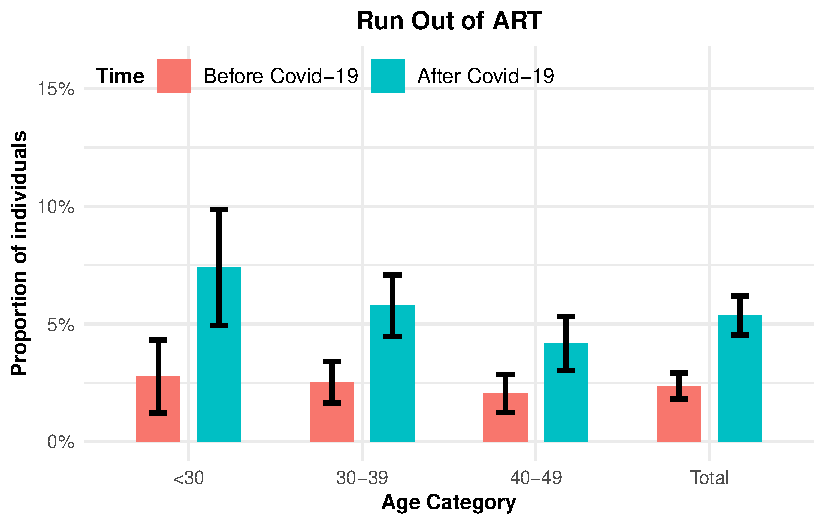
\includegraphics[keepaspectratio]{Rakai_revision_files/figure-pdf/unnamed-chunk-60-1.pdf}}

\subsubsection{Missed Scheduled Visits by Age
Category}\label{missed-scheduled-visits-by-age-category}

\begin{Shaded}
\begin{Highlighting}[]
\NormalTok{df\_age }\SpecialCharTok{\%\textgreater{}\%} \FunctionTok{group\_by}\NormalTok{(age\_cat,hivbc) }\SpecialCharTok{\%\textgreater{}\%} 
  \FunctionTok{count}\NormalTok{()}
\end{Highlighting}
\end{Shaded}

\begin{longtable}[]{@{}llr@{}}
\toprule\noalign{}
age\_cat & hivbc & n \\
\midrule\noalign{}
\endhead
\bottomrule\noalign{}
\endlastfoot
\textless30 & No & 411 \\
\textless30 & Yes & 22 \\
30-39 & No & 1186 \\
30-39 & Yes & 43 \\
40-49 & No & 1142 \\
40-49 & Yes & 30 \\
\end{longtable}

\begin{Shaded}
\begin{Highlighting}[]
\NormalTok{df\_age }\SpecialCharTok{\%\textgreater{}\%} \FunctionTok{group\_by}\NormalTok{(age\_cat,hivac) }\SpecialCharTok{\%\textgreater{}\%} 
  \FunctionTok{count}\NormalTok{()}
\end{Highlighting}
\end{Shaded}

\begin{longtable}[]{@{}llr@{}}
\toprule\noalign{}
age\_cat & hivac & n \\
\midrule\noalign{}
\endhead
\bottomrule\noalign{}
\endlastfoot
\textless30 & No & 383 \\
\textless30 & Yes & 50 \\
30-39 & No & 1095 \\
30-39 & Yes & 134 \\
40-49 & No & 1081 \\
40-49 & Yes & 91 \\
\end{longtable}

\begin{Shaded}
\begin{Highlighting}[]
\NormalTok{df\_age\_hiv }\OtherTok{\textless{}{-}}\NormalTok{ df\_age }\SpecialCharTok{\%\textgreater{}\%}
  \FunctionTok{mutate}\NormalTok{(}
    \AttributeTok{hivbc =} \FunctionTok{as.character}\NormalTok{(hivbc),}
    \AttributeTok{hivac =} \FunctionTok{as.character}\NormalTok{(hivac)}
\NormalTok{  ) }\SpecialCharTok{\%\textgreater{}\%}
  \FunctionTok{pivot\_longer}\NormalTok{(}
    \AttributeTok{cols =} \FunctionTok{c}\NormalTok{(hivbc, hivac),}
    \AttributeTok{names\_to =} \StringTok{"variable"}\NormalTok{,}
    \AttributeTok{values\_to =} \StringTok{"response"}
\NormalTok{  ) }\SpecialCharTok{\%\textgreater{}\%}
  \FunctionTok{mutate}\NormalTok{(}
    \AttributeTok{time =} \FunctionTok{if\_else}\NormalTok{(}\FunctionTok{grepl}\NormalTok{(}\StringTok{"bc$"}\NormalTok{, variable), }\StringTok{"Before Covid{-}19"}\NormalTok{, }\StringTok{"After Covid{-}19"}\NormalTok{)}
\NormalTok{  )}

\NormalTok{df\_age\_hiv\_summary }\OtherTok{\textless{}{-}}\NormalTok{ df\_age\_hiv }\SpecialCharTok{\%\textgreater{}\%}
  \FunctionTok{group\_by}\NormalTok{(time, age\_cat) }\SpecialCharTok{\%\textgreater{}\%}
  \FunctionTok{summarise}\NormalTok{(}
    \AttributeTok{n\_yes =} \FunctionTok{sum}\NormalTok{(response }\SpecialCharTok{==} \StringTok{"Yes"}\NormalTok{, }\AttributeTok{na.rm =} \ConstantTok{TRUE}\NormalTok{),}
    \AttributeTok{n =} \FunctionTok{n}\NormalTok{(),}
    \AttributeTok{.groups =} \StringTok{"drop"}
\NormalTok{  )}

\NormalTok{df\_age\_hiv\_totals }\OtherTok{\textless{}{-}}\NormalTok{ df\_age\_hiv }\SpecialCharTok{\%\textgreater{}\%}
  \FunctionTok{group\_by}\NormalTok{(time) }\SpecialCharTok{\%\textgreater{}\%}
  \FunctionTok{summarise}\NormalTok{(}
    \AttributeTok{n\_yes =} \FunctionTok{sum}\NormalTok{(response }\SpecialCharTok{==} \StringTok{"Yes"}\NormalTok{, }\AttributeTok{na.rm =} \ConstantTok{TRUE}\NormalTok{),}
    \AttributeTok{n =} \FunctionTok{n}\NormalTok{(),}
    \AttributeTok{.groups =} \StringTok{"drop"}
\NormalTok{  ) }

\NormalTok{df\_age\_hiv\_summary }\OtherTok{\textless{}{-}} \FunctionTok{bind\_rows}\NormalTok{(df\_age\_hiv\_summary, df\_age\_hiv\_totals) }\SpecialCharTok{\%\textgreater{}\%}
  \FunctionTok{mutate}\NormalTok{(}
    \AttributeTok{proportion =}\NormalTok{ n\_yes }\SpecialCharTok{/}\NormalTok{ n,}
    \AttributeTok{se =} \FunctionTok{sqrt}\NormalTok{(proportion }\SpecialCharTok{*}\NormalTok{ (}\DecValTok{1} \SpecialCharTok{{-}}\NormalTok{ proportion) }\SpecialCharTok{/}\NormalTok{ n),}
    \AttributeTok{lower =}\NormalTok{ proportion }\SpecialCharTok{{-}} \FloatTok{1.96} \SpecialCharTok{*}\NormalTok{ se,}
    \AttributeTok{upper =}\NormalTok{ proportion }\SpecialCharTok{+} \FloatTok{1.96} \SpecialCharTok{*}\NormalTok{ se}
\NormalTok{  ) }\SpecialCharTok{\%\textgreater{}\%} 
  \FunctionTok{mutate}\NormalTok{(}
    \AttributeTok{time =} \FunctionTok{as\_factor}\NormalTok{(time) }\SpecialCharTok{\%\textgreater{}\%} 
      \FunctionTok{fct\_relevel}\NormalTok{(}\StringTok{"Before Covid{-}19"}\NormalTok{),}
    \AttributeTok{age\_cat =} \FunctionTok{if\_else}\NormalTok{(}\FunctionTok{is.na}\NormalTok{(age\_cat), }\StringTok{"Total"}\NormalTok{, age\_cat)}
\NormalTok{  )}

\NormalTok{df\_age\_hiv\_summary}
\end{Highlighting}
\end{Shaded}

\begin{longtable}[]{@{}
  >{\raggedright\arraybackslash}p{(\linewidth - 14\tabcolsep) * \real{0.2105}}
  >{\raggedright\arraybackslash}p{(\linewidth - 14\tabcolsep) * \real{0.1053}}
  >{\raggedleft\arraybackslash}p{(\linewidth - 14\tabcolsep) * \real{0.0789}}
  >{\raggedleft\arraybackslash}p{(\linewidth - 14\tabcolsep) * \real{0.0658}}
  >{\raggedleft\arraybackslash}p{(\linewidth - 14\tabcolsep) * \real{0.1447}}
  >{\raggedleft\arraybackslash}p{(\linewidth - 14\tabcolsep) * \real{0.1316}}
  >{\raggedleft\arraybackslash}p{(\linewidth - 14\tabcolsep) * \real{0.1316}}
  >{\raggedleft\arraybackslash}p{(\linewidth - 14\tabcolsep) * \real{0.1316}}@{}}
\toprule\noalign{}
\begin{minipage}[b]{\linewidth}\raggedright
time
\end{minipage} & \begin{minipage}[b]{\linewidth}\raggedright
age\_cat
\end{minipage} & \begin{minipage}[b]{\linewidth}\raggedleft
n\_yes
\end{minipage} & \begin{minipage}[b]{\linewidth}\raggedleft
n
\end{minipage} & \begin{minipage}[b]{\linewidth}\raggedleft
proportion
\end{minipage} & \begin{minipage}[b]{\linewidth}\raggedleft
se
\end{minipage} & \begin{minipage}[b]{\linewidth}\raggedleft
lower
\end{minipage} & \begin{minipage}[b]{\linewidth}\raggedleft
upper
\end{minipage} \\
\midrule\noalign{}
\endhead
\bottomrule\noalign{}
\endlastfoot
After Covid-19 & \textless30 & 50 & 433 & 0.1154734 & 0.0153586 &
0.0853705 & 0.1455764 \\
After Covid-19 & 30-39 & 134 & 1229 & 0.1090317 & 0.0088906 & 0.0916061
& 0.1264573 \\
After Covid-19 & 40-49 & 91 & 1172 & 0.0776451 & 0.0078170 & 0.0623237 &
0.0929664 \\
Before Covid-19 & \textless30 & 22 & 433 & 0.0508083 & 0.0105536 &
0.0301233 & 0.0714934 \\
Before Covid-19 & 30-39 & 43 & 1229 & 0.0349878 & 0.0052414 & 0.0247146
& 0.0452610 \\
Before Covid-19 & 40-49 & 30 & 1172 & 0.0255973 & 0.0046132 & 0.0165554
& 0.0346391 \\
After Covid-19 & Total & 275 & 2834 & 0.0970360 & 0.0055603 & 0.0861377
& 0.1079343 \\
Before Covid-19 & Total & 95 & 2834 & 0.0335215 & 0.0033811 & 0.0268946
& 0.0401485 \\
\end{longtable}

\begin{Shaded}
\begin{Highlighting}[]
\NormalTok{missed\_scheduled\_visit\_by\_age\_plot }\OtherTok{\textless{}{-}} \FunctionTok{ggplot}\NormalTok{(df\_age\_hiv\_summary, }\FunctionTok{aes}\NormalTok{(}\AttributeTok{x =}\NormalTok{ age\_cat, }\AttributeTok{y =}\NormalTok{ proportion, }\AttributeTok{fill =}\NormalTok{ time)) }\SpecialCharTok{+}
  \FunctionTok{geom\_col}\NormalTok{(}\AttributeTok{position =} \FunctionTok{position\_dodge}\NormalTok{(}\AttributeTok{width =} \FloatTok{0.7}\NormalTok{), }\AttributeTok{width =} \FloatTok{0.5}\NormalTok{) }\SpecialCharTok{+}
  \FunctionTok{geom\_errorbar}\NormalTok{(}
    \FunctionTok{aes}\NormalTok{(}\AttributeTok{ymin =}\NormalTok{ lower, }\AttributeTok{ymax =}\NormalTok{ upper),}
    \AttributeTok{position =} \FunctionTok{position\_dodge}\NormalTok{(}\AttributeTok{width =} \FloatTok{0.7}\NormalTok{),}
    \AttributeTok{width =} \FloatTok{0.2}\NormalTok{,}
    \AttributeTok{size =} \DecValTok{1}
\NormalTok{  ) }\SpecialCharTok{+}
  \FunctionTok{scale\_y\_continuous}\NormalTok{(}\AttributeTok{labels =}\NormalTok{ scales}\SpecialCharTok{::}\FunctionTok{percent\_format}\NormalTok{(}\AttributeTok{accuracy =} \DecValTok{1}\NormalTok{), }\AttributeTok{limits =} \FunctionTok{c}\NormalTok{(}\DecValTok{0}\NormalTok{, }\FloatTok{0.16}\NormalTok{)) }\SpecialCharTok{+}
  \FunctionTok{labs}\NormalTok{(}
    \AttributeTok{title =} \StringTok{"Missed Scheduled Visits"}\NormalTok{,}
    \AttributeTok{x =} \StringTok{"Age Category"}\NormalTok{,}
    \AttributeTok{y =} \StringTok{"Proportion of individuals"}\NormalTok{,}
    \AttributeTok{fill =} \StringTok{"Time"}
\NormalTok{  ) }\SpecialCharTok{+}
  \FunctionTok{theme\_minimal}\NormalTok{() }\SpecialCharTok{+}
  \FunctionTok{theme}\NormalTok{(}
    \AttributeTok{plot.title =} \FunctionTok{element\_text}\NormalTok{(}\AttributeTok{hjust =} \FloatTok{0.5}\NormalTok{, }\AttributeTok{face =} \StringTok{"bold"}\NormalTok{, }\AttributeTok{size =} \DecValTok{12}\NormalTok{),}
    \AttributeTok{axis.title.x =} \FunctionTok{element\_text}\NormalTok{(}\AttributeTok{face =} \StringTok{"bold"}\NormalTok{, }\AttributeTok{size =} \DecValTok{10}\NormalTok{),}
    \AttributeTok{axis.title.y =} \FunctionTok{element\_text}\NormalTok{(}\AttributeTok{face =} \StringTok{"bold"}\NormalTok{, }\AttributeTok{size =} \DecValTok{10}\NormalTok{),}
    \AttributeTok{legend.title =} \FunctionTok{element\_text}\NormalTok{(}\AttributeTok{face =} \StringTok{"bold"}\NormalTok{, }\AttributeTok{size =} \DecValTok{10}\NormalTok{),}
    \AttributeTok{legend.text =} \FunctionTok{element\_text}\NormalTok{(}\AttributeTok{size =} \DecValTok{10}\NormalTok{),}
    \AttributeTok{legend.position =} \FunctionTok{c}\NormalTok{(}\DecValTok{0}\NormalTok{, }\DecValTok{1}\NormalTok{),}
    \AttributeTok{legend.justification =} \FunctionTok{c}\NormalTok{(}\DecValTok{0}\NormalTok{, }\DecValTok{1}\NormalTok{),}
    \AttributeTok{legend.direction =} \StringTok{"horizontal"}
\NormalTok{  )}

\NormalTok{missed\_scheduled\_visit\_by\_age\_plot}
\end{Highlighting}
\end{Shaded}

\pandocbounded{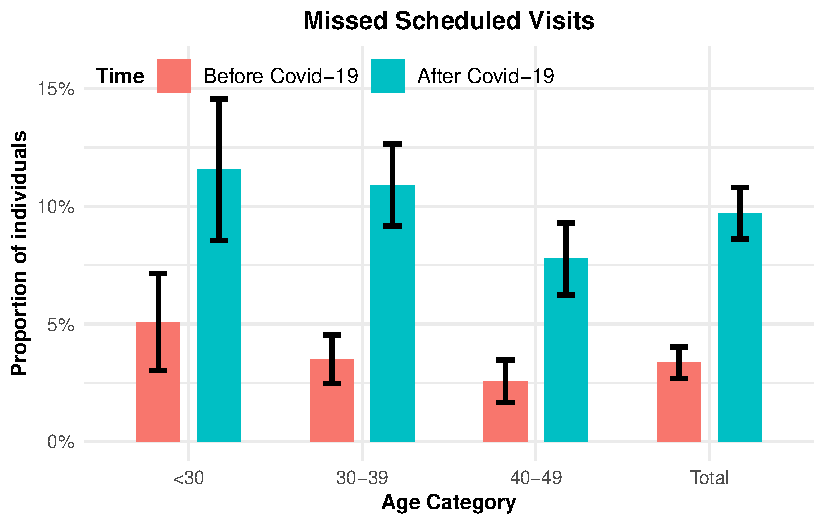
\includegraphics[keepaspectratio]{Rakai_revision_files/figure-pdf/unnamed-chunk-63-1.pdf}}

\subsubsection{Reduced ART Intake by Age
Category}\label{reduced-art-intake-by-age-category}

\begin{Shaded}
\begin{Highlighting}[]
\NormalTok{df\_age }\SpecialCharTok{\%\textgreater{}\%} \FunctionTok{group\_by}\NormalTok{(age\_cat,artstrbc) }\SpecialCharTok{\%\textgreater{}\%} 
  \FunctionTok{count}\NormalTok{()}
\end{Highlighting}
\end{Shaded}

\begin{longtable}[]{@{}llr@{}}
\toprule\noalign{}
age\_cat & artstrbc & n \\
\midrule\noalign{}
\endhead
\bottomrule\noalign{}
\endlastfoot
\textless30 & No & 426 \\
\textless30 & Yes & 7 \\
30-39 & No & 1213 \\
30-39 & Yes & 16 \\
40-49 & No & 1163 \\
40-49 & Yes & 9 \\
\end{longtable}

\begin{Shaded}
\begin{Highlighting}[]
\NormalTok{df\_age }\SpecialCharTok{\%\textgreater{}\%} \FunctionTok{group\_by}\NormalTok{(age\_cat,artstrac) }\SpecialCharTok{\%\textgreater{}\%} 
  \FunctionTok{count}\NormalTok{()}
\end{Highlighting}
\end{Shaded}

\begin{longtable}[]{@{}llr@{}}
\toprule\noalign{}
age\_cat & artstrac & n \\
\midrule\noalign{}
\endhead
\bottomrule\noalign{}
\endlastfoot
\textless30 & No & 418 \\
\textless30 & Yes & 15 \\
30-39 & No & 1190 \\
30-39 & Yes & 39 \\
40-49 & No & 1152 \\
40-49 & Yes & 20 \\
\end{longtable}

\begin{Shaded}
\begin{Highlighting}[]
\NormalTok{df\_age\_artstr }\OtherTok{\textless{}{-}}\NormalTok{ df\_age }\SpecialCharTok{\%\textgreater{}\%}
  \FunctionTok{pivot\_longer}\NormalTok{(}
    \AttributeTok{cols =} \FunctionTok{c}\NormalTok{(artstrbc, artstrac),}
    \AttributeTok{names\_to =} \StringTok{"variable"}\NormalTok{,}
    \AttributeTok{values\_to =} \StringTok{"response"}
\NormalTok{  ) }\SpecialCharTok{\%\textgreater{}\%}
  \FunctionTok{mutate}\NormalTok{(}
    \AttributeTok{time =} \FunctionTok{if\_else}\NormalTok{(}\FunctionTok{grepl}\NormalTok{(}\StringTok{"bc$"}\NormalTok{, variable), }\StringTok{"Before Covid{-}19"}\NormalTok{, }\StringTok{"After Covid{-}19"}\NormalTok{)}
\NormalTok{  )}

\NormalTok{df\_age\_artstr\_summary }\OtherTok{\textless{}{-}}\NormalTok{ df\_age\_artstr }\SpecialCharTok{\%\textgreater{}\%}
  \FunctionTok{group\_by}\NormalTok{(time, age\_cat) }\SpecialCharTok{\%\textgreater{}\%}
  \FunctionTok{summarise}\NormalTok{(}
    \AttributeTok{n\_yes =} \FunctionTok{sum}\NormalTok{(response }\SpecialCharTok{==} \StringTok{"Yes"}\NormalTok{, }\AttributeTok{na.rm =} \ConstantTok{TRUE}\NormalTok{),}
    \AttributeTok{n =} \FunctionTok{n}\NormalTok{(),}
    \AttributeTok{.groups =} \StringTok{"drop"}
\NormalTok{  )}

\NormalTok{df\_age\_artstr\_totals }\OtherTok{\textless{}{-}}\NormalTok{ df\_age\_artstr }\SpecialCharTok{\%\textgreater{}\%}
  \FunctionTok{group\_by}\NormalTok{(time) }\SpecialCharTok{\%\textgreater{}\%}
  \FunctionTok{summarise}\NormalTok{(}
    \AttributeTok{n\_yes =} \FunctionTok{sum}\NormalTok{(response }\SpecialCharTok{==} \StringTok{"Yes"}\NormalTok{, }\AttributeTok{na.rm =} \ConstantTok{TRUE}\NormalTok{),}
    \AttributeTok{n =} \FunctionTok{n}\NormalTok{(),}
    \AttributeTok{.groups =} \StringTok{"drop"}
\NormalTok{  ) }

\NormalTok{df\_age\_artstr\_summary }\OtherTok{\textless{}{-}} \FunctionTok{bind\_rows}\NormalTok{(df\_age\_artstr\_summary, df\_age\_artstr\_totals) }\SpecialCharTok{\%\textgreater{}\%}
  \FunctionTok{mutate}\NormalTok{(}
    \AttributeTok{proportion =}\NormalTok{ n\_yes }\SpecialCharTok{/}\NormalTok{ n,}
    \AttributeTok{se =} \FunctionTok{sqrt}\NormalTok{(proportion }\SpecialCharTok{*}\NormalTok{ (}\DecValTok{1} \SpecialCharTok{{-}}\NormalTok{ proportion) }\SpecialCharTok{/}\NormalTok{ n),}
    \AttributeTok{lower =}\NormalTok{ proportion }\SpecialCharTok{{-}} \FloatTok{1.96} \SpecialCharTok{*}\NormalTok{ se,}
    \AttributeTok{upper =}\NormalTok{ proportion }\SpecialCharTok{+} \FloatTok{1.96} \SpecialCharTok{*}\NormalTok{ se}
\NormalTok{  ) }\SpecialCharTok{\%\textgreater{}\%} 
  \FunctionTok{mutate}\NormalTok{(}
    \AttributeTok{time =} \FunctionTok{as\_factor}\NormalTok{(time) }\SpecialCharTok{\%\textgreater{}\%} 
      \FunctionTok{fct\_relevel}\NormalTok{(}\StringTok{"Before Covid{-}19"}\NormalTok{),}
    \AttributeTok{age\_cat =} \FunctionTok{if\_else}\NormalTok{(}\FunctionTok{is.na}\NormalTok{(age\_cat), }\StringTok{"Total"}\NormalTok{, age\_cat)}
\NormalTok{  )}

\NormalTok{df\_age\_artstr\_summary}
\end{Highlighting}
\end{Shaded}

\begin{longtable}[]{@{}
  >{\raggedright\arraybackslash}p{(\linewidth - 14\tabcolsep) * \real{0.2105}}
  >{\raggedright\arraybackslash}p{(\linewidth - 14\tabcolsep) * \real{0.1053}}
  >{\raggedleft\arraybackslash}p{(\linewidth - 14\tabcolsep) * \real{0.0789}}
  >{\raggedleft\arraybackslash}p{(\linewidth - 14\tabcolsep) * \real{0.0658}}
  >{\raggedleft\arraybackslash}p{(\linewidth - 14\tabcolsep) * \real{0.1447}}
  >{\raggedleft\arraybackslash}p{(\linewidth - 14\tabcolsep) * \real{0.1316}}
  >{\raggedleft\arraybackslash}p{(\linewidth - 14\tabcolsep) * \real{0.1316}}
  >{\raggedleft\arraybackslash}p{(\linewidth - 14\tabcolsep) * \real{0.1316}}@{}}
\toprule\noalign{}
\begin{minipage}[b]{\linewidth}\raggedright
time
\end{minipage} & \begin{minipage}[b]{\linewidth}\raggedright
age\_cat
\end{minipage} & \begin{minipage}[b]{\linewidth}\raggedleft
n\_yes
\end{minipage} & \begin{minipage}[b]{\linewidth}\raggedleft
n
\end{minipage} & \begin{minipage}[b]{\linewidth}\raggedleft
proportion
\end{minipage} & \begin{minipage}[b]{\linewidth}\raggedleft
se
\end{minipage} & \begin{minipage}[b]{\linewidth}\raggedleft
lower
\end{minipage} & \begin{minipage}[b]{\linewidth}\raggedleft
upper
\end{minipage} \\
\midrule\noalign{}
\endhead
\bottomrule\noalign{}
\endlastfoot
After Covid-19 & \textless30 & 15 & 433 & 0.0346420 & 0.0087882 &
0.0174171 & 0.0518670 \\
After Covid-19 & 30-39 & 39 & 1229 & 0.0317331 & 0.0050001 & 0.0219329 &
0.0415333 \\
After Covid-19 & 40-49 & 20 & 1172 & 0.0170648 & 0.0037831 & 0.0096499 &
0.0244798 \\
Before Covid-19 & \textless30 & 7 & 433 & 0.0161663 & 0.0060607 &
0.0042873 & 0.0280452 \\
Before Covid-19 & 30-39 & 16 & 1229 & 0.0130187 & 0.0032334 & 0.0066812
& 0.0193562 \\
Before Covid-19 & 40-49 & 9 & 1172 & 0.0076792 & 0.0025499 & 0.0026814 &
0.0126769 \\
After Covid-19 & Total & 74 & 2834 & 0.0261115 & 0.0029955 & 0.0202403 &
0.0319827 \\
Before Covid-19 & Total & 32 & 2834 & 0.0112915 & 0.0019848 & 0.0074013
& 0.0151816 \\
\end{longtable}

\begin{Shaded}
\begin{Highlighting}[]
\NormalTok{reduced\_art\_intake\_by\_age\_plot }\OtherTok{\textless{}{-}} \FunctionTok{ggplot}\NormalTok{(df\_age\_artstr\_summary, }\FunctionTok{aes}\NormalTok{(}\AttributeTok{x =}\NormalTok{ age\_cat, }\AttributeTok{y =}\NormalTok{ proportion, }\AttributeTok{fill =}\NormalTok{ time)) }\SpecialCharTok{+}
  \FunctionTok{geom\_col}\NormalTok{(}\AttributeTok{position =} \FunctionTok{position\_dodge}\NormalTok{(}\AttributeTok{width =} \FloatTok{0.7}\NormalTok{), }\AttributeTok{width =} \FloatTok{0.5}\NormalTok{) }\SpecialCharTok{+}
  \FunctionTok{geom\_errorbar}\NormalTok{(}
    \FunctionTok{aes}\NormalTok{(}\AttributeTok{ymin =}\NormalTok{ lower, }\AttributeTok{ymax =}\NormalTok{ upper),}
    \AttributeTok{position =} \FunctionTok{position\_dodge}\NormalTok{(}\AttributeTok{width =} \FloatTok{0.7}\NormalTok{),}
    \AttributeTok{width =} \FloatTok{0.2}\NormalTok{,}
    \AttributeTok{size =} \DecValTok{1}
\NormalTok{  ) }\SpecialCharTok{+}
  \FunctionTok{scale\_y\_continuous}\NormalTok{(}\AttributeTok{labels =}\NormalTok{ scales}\SpecialCharTok{::}\FunctionTok{percent\_format}\NormalTok{(}\AttributeTok{accuracy =} \DecValTok{1}\NormalTok{), }\AttributeTok{limits =} \FunctionTok{c}\NormalTok{(}\DecValTok{0}\NormalTok{, }\FloatTok{0.16}\NormalTok{)) }\SpecialCharTok{+}
  \FunctionTok{labs}\NormalTok{(}
    \AttributeTok{title =} \StringTok{"Reduced ART Intake"}\NormalTok{,}
    \AttributeTok{x =} \StringTok{"Age Category"}\NormalTok{,}
    \AttributeTok{y =} \StringTok{"Proportion of Individuals"}\NormalTok{,}
    \AttributeTok{fill =} \StringTok{"Time"}
\NormalTok{  ) }\SpecialCharTok{+}
  \FunctionTok{theme\_minimal}\NormalTok{() }\SpecialCharTok{+}
  \FunctionTok{theme}\NormalTok{(}
    \AttributeTok{plot.title =} \FunctionTok{element\_text}\NormalTok{(}\AttributeTok{hjust =} \FloatTok{0.5}\NormalTok{, }\AttributeTok{face =} \StringTok{"bold"}\NormalTok{, }\AttributeTok{size =} \DecValTok{12}\NormalTok{),}
    \AttributeTok{axis.title.x =} \FunctionTok{element\_text}\NormalTok{(}\AttributeTok{face =} \StringTok{"bold"}\NormalTok{, }\AttributeTok{size =} \DecValTok{10}\NormalTok{),}
    \AttributeTok{axis.title.y =} \FunctionTok{element\_text}\NormalTok{(}\AttributeTok{face =} \StringTok{"bold"}\NormalTok{, }\AttributeTok{size =} \DecValTok{10}\NormalTok{),}
    \AttributeTok{legend.title =} \FunctionTok{element\_text}\NormalTok{(}\AttributeTok{face =} \StringTok{"bold"}\NormalTok{, }\AttributeTok{size =} \DecValTok{10}\NormalTok{),}
    \AttributeTok{legend.text =} \FunctionTok{element\_text}\NormalTok{(}\AttributeTok{size =} \DecValTok{10}\NormalTok{),}
    \AttributeTok{legend.position =} \FunctionTok{c}\NormalTok{(}\DecValTok{0}\NormalTok{, }\DecValTok{1}\NormalTok{),}
    \AttributeTok{legend.justification =} \FunctionTok{c}\NormalTok{(}\DecValTok{0}\NormalTok{, }\DecValTok{1}\NormalTok{),}
    \AttributeTok{legend.direction =} \StringTok{"horizontal"}
\NormalTok{  )}

\NormalTok{reduced\_art\_intake\_by\_age\_plot}
\end{Highlighting}
\end{Shaded}

\pandocbounded{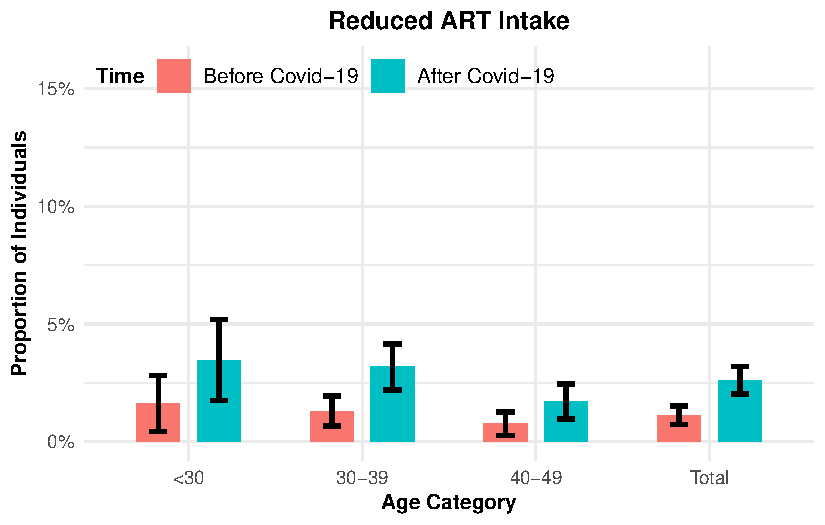
\includegraphics[keepaspectratio]{Rakai_revision_files/figure-pdf/unnamed-chunk-66-1.pdf}}

\begin{Shaded}
\begin{Highlighting}[]
\NormalTok{pa1 }\OtherTok{\textless{}{-}} \FunctionTok{ggplot}\NormalTok{(df\_age\_artstr\_summary, }\FunctionTok{aes}\NormalTok{(}\AttributeTok{x =}\NormalTok{ age\_cat, }\AttributeTok{y =}\NormalTok{ proportion, }\AttributeTok{fill =}\NormalTok{ time)) }\SpecialCharTok{+}
  \FunctionTok{geom\_col}\NormalTok{(}\AttributeTok{position =} \FunctionTok{position\_dodge}\NormalTok{(}\AttributeTok{width =} \FloatTok{0.7}\NormalTok{), }\AttributeTok{width =} \FloatTok{0.5}\NormalTok{) }\SpecialCharTok{+}
  \FunctionTok{geom\_errorbar}\NormalTok{(}
    \FunctionTok{aes}\NormalTok{(}\AttributeTok{ymin =}\NormalTok{ lower, }\AttributeTok{ymax =}\NormalTok{ upper),}
    \AttributeTok{position =} \FunctionTok{position\_dodge}\NormalTok{(}\AttributeTok{width =} \FloatTok{0.7}\NormalTok{),}
    \AttributeTok{width =} \FloatTok{0.2}\NormalTok{,}
    \AttributeTok{size =} \DecValTok{1}
\NormalTok{  ) }\SpecialCharTok{+}
  \FunctionTok{scale\_y\_continuous}\NormalTok{(}\AttributeTok{labels =}\NormalTok{ scales}\SpecialCharTok{::}\FunctionTok{percent\_format}\NormalTok{(}\AttributeTok{accuracy =} \DecValTok{1}\NormalTok{), }\AttributeTok{limits =} \FunctionTok{c}\NormalTok{(}\DecValTok{0}\NormalTok{, }\FloatTok{0.25}\NormalTok{)) }\SpecialCharTok{+}
  \FunctionTok{labs}\NormalTok{(}
    \AttributeTok{title =} \StringTok{"Reduced ART Intake"}\NormalTok{,}
    \AttributeTok{x =} \StringTok{"Age Category"}\NormalTok{,}
    \AttributeTok{y =} \StringTok{"Proportion of individuals"}\NormalTok{,}
    \AttributeTok{fill =} \StringTok{"Time"}
\NormalTok{  ) }\SpecialCharTok{+}
  \FunctionTok{theme\_minimal}\NormalTok{() }\SpecialCharTok{+}
  \FunctionTok{theme}\NormalTok{(}
    \AttributeTok{plot.title =} \FunctionTok{element\_text}\NormalTok{(}\AttributeTok{hjust =} \FloatTok{0.5}\NormalTok{, }\AttributeTok{face =} \StringTok{"bold"}\NormalTok{, }\AttributeTok{size =} \DecValTok{12}\NormalTok{),}
    \AttributeTok{axis.title.x =} \FunctionTok{element\_text}\NormalTok{(}\AttributeTok{face =} \StringTok{"bold"}\NormalTok{, }\AttributeTok{size =} \DecValTok{10}\NormalTok{),}
    \AttributeTok{axis.title.y =} \FunctionTok{element\_text}\NormalTok{(}\AttributeTok{face =} \StringTok{"bold"}\NormalTok{, }\AttributeTok{size =} \DecValTok{10}\NormalTok{),}
    \AttributeTok{legend.title =} \FunctionTok{element\_text}\NormalTok{(}\AttributeTok{face =} \StringTok{"bold"}\NormalTok{, }\AttributeTok{size =} \DecValTok{10}\NormalTok{),}
    \AttributeTok{legend.text =} \FunctionTok{element\_text}\NormalTok{(}\AttributeTok{size =} \DecValTok{10}\NormalTok{),}
    \AttributeTok{legend.position =} \FunctionTok{c}\NormalTok{(}\DecValTok{0}\NormalTok{, }\DecValTok{1}\NormalTok{),}
    \AttributeTok{legend.justification =} \FunctionTok{c}\NormalTok{(}\DecValTok{0}\NormalTok{, }\DecValTok{1}\NormalTok{),}
    \AttributeTok{legend.direction =} \StringTok{"horizontal"}
\NormalTok{  )}
\NormalTok{pa1}
\end{Highlighting}
\end{Shaded}

\pandocbounded{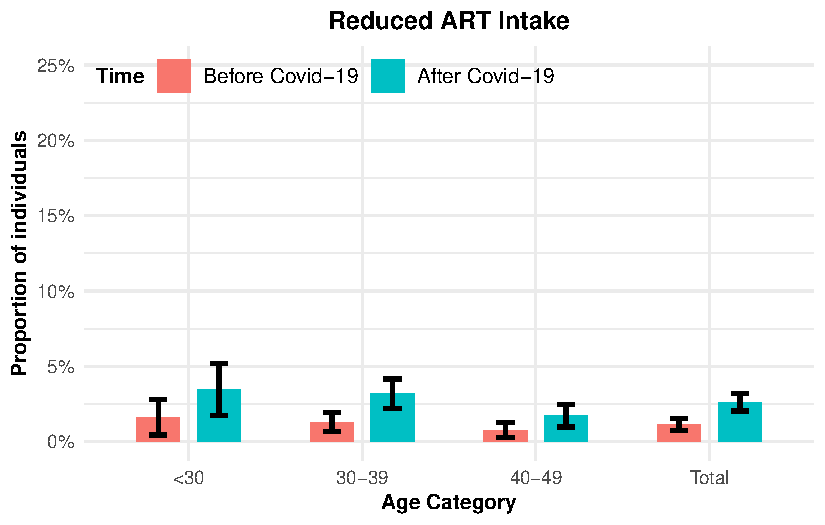
\includegraphics[keepaspectratio]{Rakai_revision_files/figure-pdf/unnamed-chunk-67-1.pdf}}

\begin{Shaded}
\begin{Highlighting}[]
\NormalTok{pa2 }\OtherTok{\textless{}{-}} \FunctionTok{ggplot}\NormalTok{(df\_age\_hiv\_summary, }\FunctionTok{aes}\NormalTok{(}\AttributeTok{x =}\NormalTok{ age\_cat, }\AttributeTok{y =}\NormalTok{ proportion, }\AttributeTok{fill =}\NormalTok{ time)) }\SpecialCharTok{+}
  \FunctionTok{geom\_col}\NormalTok{(}\AttributeTok{position =} \FunctionTok{position\_dodge}\NormalTok{(}\AttributeTok{width =} \FloatTok{0.7}\NormalTok{), }\AttributeTok{width =} \FloatTok{0.5}\NormalTok{) }\SpecialCharTok{+}
  \FunctionTok{geom\_errorbar}\NormalTok{(}
    \FunctionTok{aes}\NormalTok{(}\AttributeTok{ymin =}\NormalTok{ lower, }\AttributeTok{ymax =}\NormalTok{ upper),}
    \AttributeTok{position =} \FunctionTok{position\_dodge}\NormalTok{(}\AttributeTok{width =} \FloatTok{0.7}\NormalTok{),}
    \AttributeTok{width =} \FloatTok{0.2}\NormalTok{,}
    \AttributeTok{size =} \DecValTok{1}
\NormalTok{  ) }\SpecialCharTok{+}
  \FunctionTok{scale\_y\_continuous}\NormalTok{(}\AttributeTok{labels =}\NormalTok{ scales}\SpecialCharTok{::}\FunctionTok{percent\_format}\NormalTok{(}\AttributeTok{accuracy =} \DecValTok{1}\NormalTok{), }\AttributeTok{limits =} \FunctionTok{c}\NormalTok{(}\DecValTok{0}\NormalTok{, }\FloatTok{0.25}\NormalTok{)) }\SpecialCharTok{+}
  \FunctionTok{labs}\NormalTok{(}
    \AttributeTok{title =} \StringTok{"Missed Scheduled Visits"}\NormalTok{,}
    \AttributeTok{x =} \StringTok{"Age Category"}\NormalTok{,}
    \AttributeTok{y =} \StringTok{"Proportion of individuals"}\NormalTok{,}
    \AttributeTok{fill =} \StringTok{"Time"}
\NormalTok{  ) }\SpecialCharTok{+}
  \FunctionTok{theme\_minimal}\NormalTok{() }\SpecialCharTok{+}
  \FunctionTok{theme}\NormalTok{(}
    \AttributeTok{plot.title =} \FunctionTok{element\_text}\NormalTok{(}\AttributeTok{hjust =} \FloatTok{0.5}\NormalTok{, }\AttributeTok{face =} \StringTok{"bold"}\NormalTok{, }\AttributeTok{size =} \DecValTok{12}\NormalTok{),}
    \AttributeTok{axis.title.x =} \FunctionTok{element\_text}\NormalTok{(}\AttributeTok{face =} \StringTok{"bold"}\NormalTok{, }\AttributeTok{size =} \DecValTok{10}\NormalTok{),}
    \AttributeTok{axis.title.y =} \FunctionTok{element\_text}\NormalTok{(}\AttributeTok{face =} \StringTok{"bold"}\NormalTok{, }\AttributeTok{size =} \DecValTok{10}\NormalTok{),}
    \AttributeTok{legend.title =} \FunctionTok{element\_text}\NormalTok{(}\AttributeTok{face =} \StringTok{"bold"}\NormalTok{, }\AttributeTok{size =} \DecValTok{10}\NormalTok{),}
    \AttributeTok{legend.text =} \FunctionTok{element\_text}\NormalTok{(}\AttributeTok{size =} \DecValTok{10}\NormalTok{),}
    \AttributeTok{legend.position =} \FunctionTok{c}\NormalTok{(}\DecValTok{0}\NormalTok{, }\DecValTok{1}\NormalTok{),}
    \AttributeTok{legend.justification =} \FunctionTok{c}\NormalTok{(}\DecValTok{0}\NormalTok{, }\DecValTok{1}\NormalTok{),}
    \AttributeTok{legend.direction =} \StringTok{"horizontal"}
\NormalTok{  )}

\NormalTok{pa2}
\end{Highlighting}
\end{Shaded}

\pandocbounded{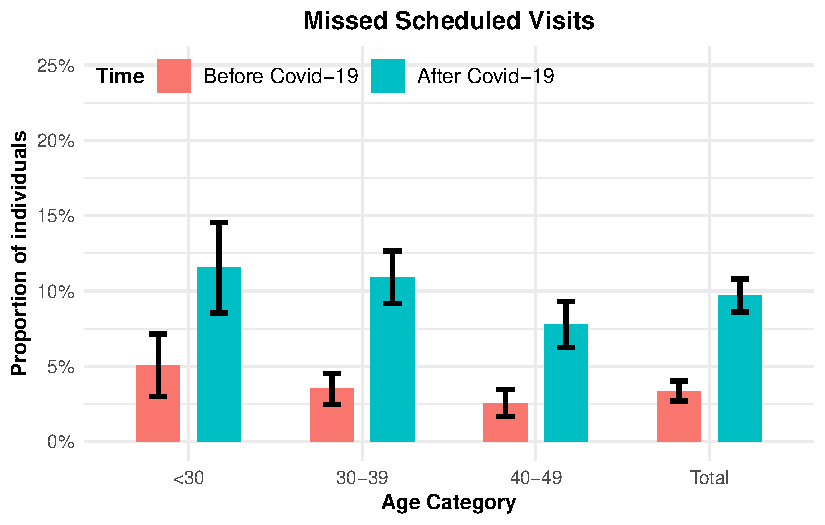
\includegraphics[keepaspectratio]{Rakai_revision_files/figure-pdf/unnamed-chunk-68-1.pdf}}

\begin{Shaded}
\begin{Highlighting}[]
\NormalTok{pa3 }\OtherTok{\textless{}{-}} \FunctionTok{ggplot}\NormalTok{(df\_age\_artrun\_summary, }\FunctionTok{aes}\NormalTok{(}\AttributeTok{x =}\NormalTok{ age\_cat, }\AttributeTok{y =}\NormalTok{ proportion, }\AttributeTok{fill =}\NormalTok{ time)) }\SpecialCharTok{+}
  \FunctionTok{geom\_col}\NormalTok{(}\AttributeTok{position =} \FunctionTok{position\_dodge}\NormalTok{(}\AttributeTok{width =} \FloatTok{0.7}\NormalTok{), }\AttributeTok{width =} \FloatTok{0.5}\NormalTok{) }\SpecialCharTok{+}
  \FunctionTok{geom\_errorbar}\NormalTok{(}
    \FunctionTok{aes}\NormalTok{(}\AttributeTok{ymin =}\NormalTok{ lower, }\AttributeTok{ymax =}\NormalTok{ upper),}
    \AttributeTok{position =} \FunctionTok{position\_dodge}\NormalTok{(}\AttributeTok{width =} \FloatTok{0.7}\NormalTok{),}
    \AttributeTok{width =} \FloatTok{0.2}\NormalTok{,}
    \AttributeTok{size =} \DecValTok{1}
\NormalTok{  ) }\SpecialCharTok{+}
  \FunctionTok{scale\_y\_continuous}\NormalTok{(}\AttributeTok{labels =}\NormalTok{ scales}\SpecialCharTok{::}\FunctionTok{percent\_format}\NormalTok{(}\AttributeTok{accuracy =} \DecValTok{1}\NormalTok{), }\AttributeTok{limits =} \FunctionTok{c}\NormalTok{(}\DecValTok{0}\NormalTok{, }\FloatTok{0.25}\NormalTok{)) }\SpecialCharTok{+}
  \FunctionTok{labs}\NormalTok{(}
   \AttributeTok{title =} \StringTok{"Run Out of ART"}\NormalTok{,}
    \AttributeTok{x =} \StringTok{"Age Category"}\NormalTok{,}
    \AttributeTok{y =} \StringTok{"Proportion of individuals"}\NormalTok{,}
    \AttributeTok{fill =} \StringTok{"Time"}
\NormalTok{  ) }\SpecialCharTok{+}
  \FunctionTok{theme\_minimal}\NormalTok{() }\SpecialCharTok{+}
  \FunctionTok{theme}\NormalTok{(}
    \AttributeTok{plot.title =} \FunctionTok{element\_text}\NormalTok{(}\AttributeTok{hjust =} \FloatTok{0.5}\NormalTok{, }\AttributeTok{face =} \StringTok{"bold"}\NormalTok{, }\AttributeTok{size =} \DecValTok{12}\NormalTok{),}
    \AttributeTok{axis.title.x =} \FunctionTok{element\_text}\NormalTok{(}\AttributeTok{face =} \StringTok{"bold"}\NormalTok{, }\AttributeTok{size =} \DecValTok{10}\NormalTok{),}
    \AttributeTok{axis.title.y =} \FunctionTok{element\_text}\NormalTok{(}\AttributeTok{face =} \StringTok{"bold"}\NormalTok{, }\AttributeTok{size =} \DecValTok{10}\NormalTok{),}
    \AttributeTok{legend.title =} \FunctionTok{element\_text}\NormalTok{(}\AttributeTok{face =} \StringTok{"bold"}\NormalTok{, }\AttributeTok{size =} \DecValTok{10}\NormalTok{),}
    \AttributeTok{legend.text =} \FunctionTok{element\_text}\NormalTok{(}\AttributeTok{size =} \DecValTok{10}\NormalTok{),}
    \AttributeTok{legend.position =} \FunctionTok{c}\NormalTok{(}\DecValTok{0}\NormalTok{, }\DecValTok{1}\NormalTok{),}
    \AttributeTok{legend.justification =} \FunctionTok{c}\NormalTok{(}\DecValTok{0}\NormalTok{, }\DecValTok{1}\NormalTok{),}
    \AttributeTok{legend.direction =} \StringTok{"horizontal"}
\NormalTok{  )}

\NormalTok{pa3}
\end{Highlighting}
\end{Shaded}

\pandocbounded{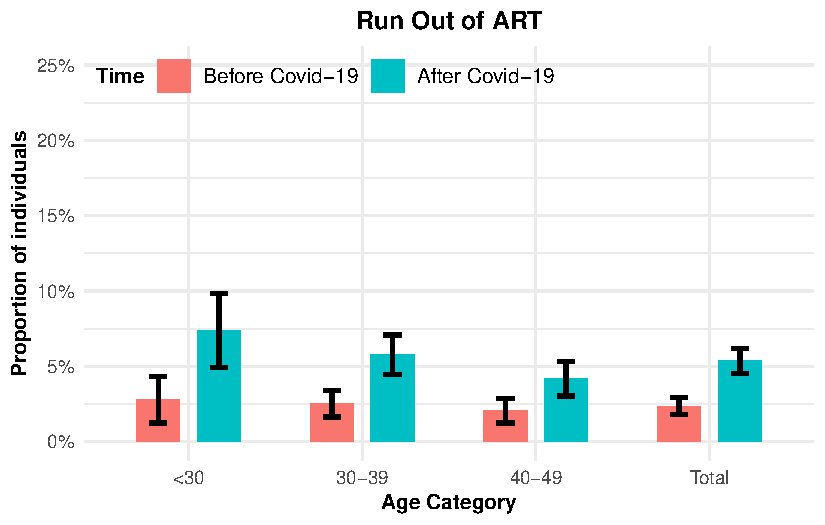
\includegraphics[keepaspectratio]{Rakai_revision_files/figure-pdf/unnamed-chunk-69-1.pdf}}

\begin{Shaded}
\begin{Highlighting}[]
\DocumentationTok{\#\#\# Combined plot}
\NormalTok{(pa1 }\SpecialCharTok{+}\NormalTok{ pa2)}\SpecialCharTok{/}\NormalTok{pa3}
\end{Highlighting}
\end{Shaded}

\pandocbounded{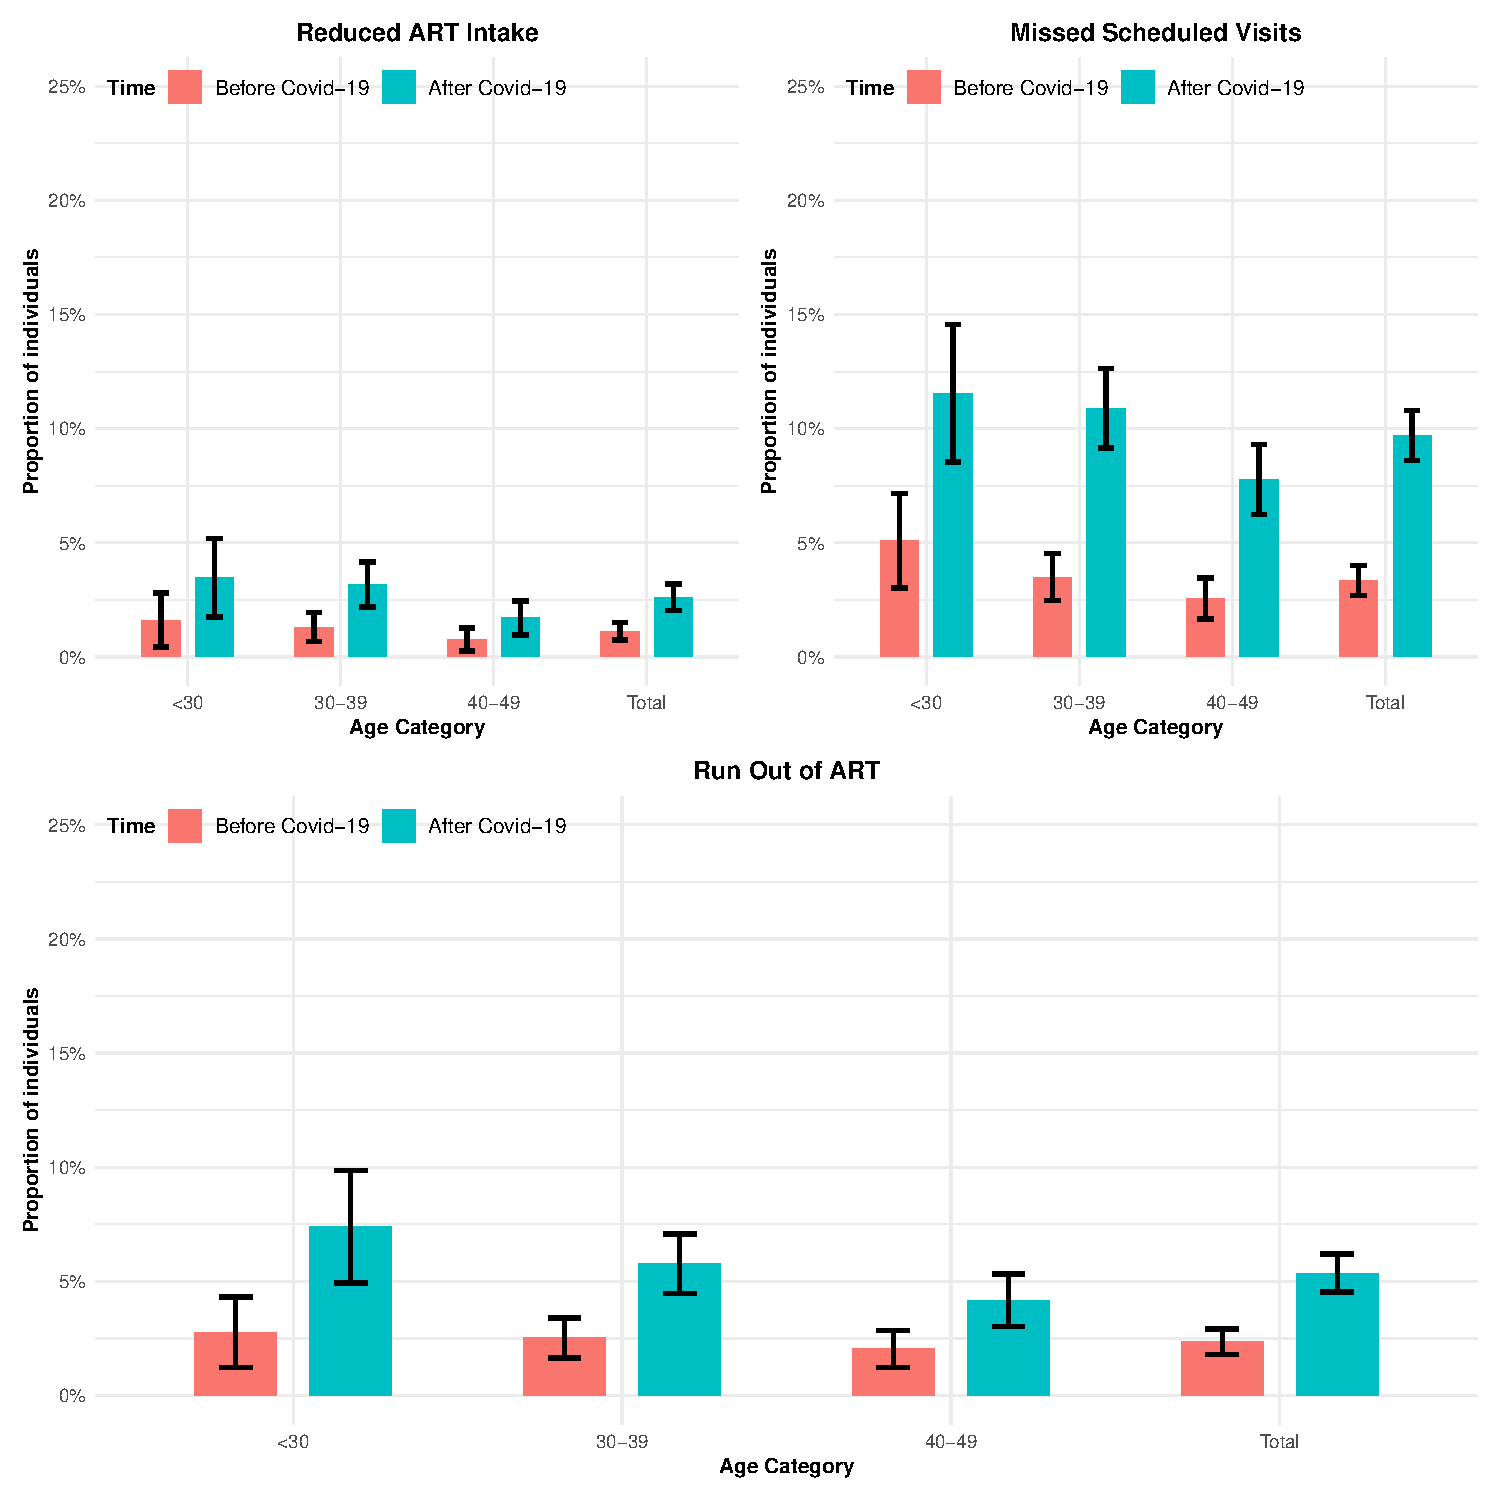
\includegraphics[keepaspectratio]{Rakai_revision_files/figure-pdf/unnamed-chunk-70-1.pdf}}

\section{ART Duration}\label{art-duration}

\begin{Shaded}
\begin{Highlighting}[]
\NormalTok{df\_dur }\OtherTok{\textless{}{-}}\NormalTok{ rakai }\SpecialCharTok{\%\textgreater{}\%} 
  \FunctionTok{select}\NormalTok{(artyrs,artrunbc,artrunac,}
\NormalTok{         hivac,hivbc,copies,new\_copies,artstrac,artstrbc) }\SpecialCharTok{\%\textgreater{}\%} 
  \FunctionTok{filter}\NormalTok{(hivac }\SpecialCharTok{!=}\DecValTok{8}\NormalTok{, hivbc}\SpecialCharTok{!=}\DecValTok{8}\NormalTok{,artrunbc}\SpecialCharTok{!=}\DecValTok{8}\NormalTok{,artstrac}\SpecialCharTok{!=}\DecValTok{8}\NormalTok{,artstrbc}\SpecialCharTok{!=}\DecValTok{8}\NormalTok{,artrunac}\SpecialCharTok{!=}\DecValTok{8}\NormalTok{) }\SpecialCharTok{\%\textgreater{}\%} 
 \FunctionTok{mutate}\NormalTok{(}
  \AttributeTok{art\_duration =} \FunctionTok{case\_when}\NormalTok{(}
\NormalTok{     artyrs }\SpecialCharTok{\textgreater{}=} \DecValTok{2} \SpecialCharTok{\&}\NormalTok{  artyrs }\SpecialCharTok{\textless{}=} \DecValTok{5} \SpecialCharTok{\textasciitilde{}} \StringTok{"2{-}5 years"}\NormalTok{,}
\NormalTok{    artyrs }\SpecialCharTok{\textgreater{}} \DecValTok{5} \SpecialCharTok{\textasciitilde{}} \StringTok{"\textgreater{}5 years"}\NormalTok{,}
    \AttributeTok{.default =}  \StringTok{"\textless{}2 years"}
\NormalTok{  ) }\SpecialCharTok{\%\textgreater{}\%} 
    \FunctionTok{fct\_relevel}\NormalTok{(}\StringTok{"\textless{}2 years"}\NormalTok{,}\StringTok{"2{-}5 years"}\NormalTok{) }\SpecialCharTok{\%\textgreater{}\%} 
    \FunctionTok{ff\_label}\NormalTok{(}\StringTok{"Time on ART"}\NormalTok{),}
  
    \AttributeTok{hivac =} \FunctionTok{if\_else}\NormalTok{(hivac }\SpecialCharTok{==}\DecValTok{1}\NormalTok{, }\StringTok{"Yes"}\NormalTok{,}\StringTok{"No"}\NormalTok{) }\SpecialCharTok{\%\textgreater{}\%} 
    \FunctionTok{ff\_label}\NormalTok{(}\StringTok{"Missed scheduled visit for HIV care"}\NormalTok{) }\SpecialCharTok{\%\textgreater{}\%} 
      \FunctionTok{as\_factor}\NormalTok{(),}
   
     \AttributeTok{hivbc =} \FunctionTok{if\_else}\NormalTok{(hivbc }\SpecialCharTok{==}\DecValTok{1}\NormalTok{,}\StringTok{"Yes"}\NormalTok{,}\StringTok{"No"}\NormalTok{) }\SpecialCharTok{\%\textgreater{}\%} 
    \FunctionTok{ff\_label}\NormalTok{(}\StringTok{"Missed scheduled visit for HIV care"}\NormalTok{) }\SpecialCharTok{\%\textgreater{}\%} 
    \FunctionTok{as\_factor}\NormalTok{(),}
 
     \AttributeTok{artrunac =} \FunctionTok{if\_else}\NormalTok{(artrunac }\SpecialCharTok{==}\DecValTok{1}\NormalTok{,}\StringTok{"Yes"}\NormalTok{,}\StringTok{"No"}\NormalTok{) }\SpecialCharTok{\%\textgreater{}\%} 
    \FunctionTok{as\_factor}\NormalTok{() }\SpecialCharTok{\%\textgreater{}\%} 
    \FunctionTok{ff\_label}\NormalTok{(}\StringTok{"Run out of ART before next refill"}\NormalTok{),}
 
   \AttributeTok{artrunbc =} \FunctionTok{if\_else}\NormalTok{(artrunbc }\SpecialCharTok{==}\DecValTok{1}\NormalTok{,}\StringTok{"Yes"}\NormalTok{,}\StringTok{"No"}\NormalTok{) }\SpecialCharTok{\%\textgreater{}\%} 
    \FunctionTok{as\_factor}\NormalTok{() }\SpecialCharTok{\%\textgreater{}\%} 
    \FunctionTok{ff\_label}\NormalTok{(}\StringTok{"Run out of ART before next refill"}\NormalTok{),}
  
  \AttributeTok{artstrac =} \FunctionTok{if\_else}\NormalTok{(artstrac }\SpecialCharTok{==}\DecValTok{1}\NormalTok{,}\StringTok{"Yes"}\NormalTok{,}\StringTok{"No"}\NormalTok{) }\SpecialCharTok{\%\textgreater{}\%} 
    \FunctionTok{as\_factor}\NormalTok{() }\SpecialCharTok{\%\textgreater{}\%} 
    \FunctionTok{ff\_label}\NormalTok{(}\StringTok{"Taken ART pills less frequently / in smaller}
\StringTok{amounts to conserve supply"}\NormalTok{),}
  
  \AttributeTok{artstrbc =} \FunctionTok{if\_else}\NormalTok{(artstrbc }\SpecialCharTok{==}\DecValTok{1}\NormalTok{,}\StringTok{"Yes"}\NormalTok{,}\StringTok{"No"}\NormalTok{) }\SpecialCharTok{\%\textgreater{}\%} 
    \FunctionTok{as\_factor}\NormalTok{() }\SpecialCharTok{\%\textgreater{}\%} 
    \FunctionTok{ff\_label}\NormalTok{(}\StringTok{"Taken ART pills less frequently / in smaller}
\StringTok{amounts to conserve supply"}\NormalTok{)}
\NormalTok{  ) }\SpecialCharTok{\%\textgreater{}\%} 
  \FunctionTok{select}\NormalTok{(}\SpecialCharTok{{-}}\NormalTok{artyrs)}
\end{Highlighting}
\end{Shaded}

\begin{Shaded}
\begin{Highlighting}[]
\CommentTok{\# df\_dur}
\end{Highlighting}
\end{Shaded}

\begin{Shaded}
\begin{Highlighting}[]
\NormalTok{df\_dur }\SpecialCharTok{\%\textgreater{}\%} \FunctionTok{group\_by}\NormalTok{(art\_duration,artstrbc) }\SpecialCharTok{\%\textgreater{}\%} 
  \FunctionTok{count}\NormalTok{()}
\end{Highlighting}
\end{Shaded}

\begin{longtable}[]{@{}llr@{}}
\toprule\noalign{}
art\_duration & artstrbc & n \\
\midrule\noalign{}
\endhead
\bottomrule\noalign{}
\endlastfoot
\textless2 years & No & 166 \\
\textless2 years & Yes & 1 \\
2-5 years & No & 868 \\
2-5 years & Yes & 12 \\
\textgreater5 years & No & 1768 \\
\textgreater5 years & Yes & 19 \\
\end{longtable}

\begin{Shaded}
\begin{Highlighting}[]
\NormalTok{df\_dur }\SpecialCharTok{\%\textgreater{}\%} \FunctionTok{group\_by}\NormalTok{(art\_duration,artstrac) }\SpecialCharTok{\%\textgreater{}\%} 
  \FunctionTok{count}\NormalTok{()}
\end{Highlighting}
\end{Shaded}

\begin{longtable}[]{@{}llr@{}}
\toprule\noalign{}
art\_duration & artstrac & n \\
\midrule\noalign{}
\endhead
\bottomrule\noalign{}
\endlastfoot
\textless2 years & No & 163 \\
\textless2 years & Yes & 4 \\
2-5 years & No & 852 \\
2-5 years & Yes & 28 \\
\textgreater5 years & No & 1745 \\
\textgreater5 years & Yes & 42 \\
\end{longtable}

\subsubsection{Reduced ART intake by ART
duration}\label{reduced-art-intake-by-art-duration}

\begin{Shaded}
\begin{Highlighting}[]
\NormalTok{df\_dur\_artstr }\OtherTok{\textless{}{-}}\NormalTok{ df\_dur }\SpecialCharTok{\%\textgreater{}\%}
  \FunctionTok{pivot\_longer}\NormalTok{(}
    \AttributeTok{cols =} \FunctionTok{c}\NormalTok{(artstrbc, artstrac),}
    \AttributeTok{names\_to =} \StringTok{"variable"}\NormalTok{,}
    \AttributeTok{values\_to =} \StringTok{"response"}
\NormalTok{  ) }\SpecialCharTok{\%\textgreater{}\%}
  \FunctionTok{mutate}\NormalTok{(}
    \AttributeTok{time =} \FunctionTok{if\_else}\NormalTok{(}\FunctionTok{grepl}\NormalTok{(}\StringTok{"bc$"}\NormalTok{, variable), }\StringTok{"Before Covid{-}19"}\NormalTok{, }\StringTok{"After Covid{-}19"}\NormalTok{)}
\NormalTok{  )}

\NormalTok{df\_dur\_artstr\_summary }\OtherTok{\textless{}{-}}\NormalTok{ df\_dur\_artstr }\SpecialCharTok{\%\textgreater{}\%}
  \FunctionTok{group\_by}\NormalTok{(time, art\_duration) }\SpecialCharTok{\%\textgreater{}\%}
  \FunctionTok{summarise}\NormalTok{(}
    \AttributeTok{n\_yes =} \FunctionTok{sum}\NormalTok{(response }\SpecialCharTok{==} \StringTok{"Yes"}\NormalTok{, }\AttributeTok{na.rm =} \ConstantTok{TRUE}\NormalTok{),}
    \AttributeTok{n =} \FunctionTok{n}\NormalTok{(),}
    \AttributeTok{.groups =} \StringTok{"drop"}
\NormalTok{  )}

\NormalTok{df\_dur\_artstr\_totals }\OtherTok{\textless{}{-}}\NormalTok{ df\_dur\_artstr }\SpecialCharTok{\%\textgreater{}\%}
  \FunctionTok{group\_by}\NormalTok{(time) }\SpecialCharTok{\%\textgreater{}\%}
  \FunctionTok{summarise}\NormalTok{(}
    \AttributeTok{n\_yes =} \FunctionTok{sum}\NormalTok{(response }\SpecialCharTok{==} \StringTok{"Yes"}\NormalTok{, }\AttributeTok{na.rm =} \ConstantTok{TRUE}\NormalTok{),}
    \AttributeTok{n =} \FunctionTok{n}\NormalTok{(),}
    \AttributeTok{.groups =} \StringTok{"drop"}
\NormalTok{  ) }

\NormalTok{df\_dur\_artstr\_summary }\OtherTok{\textless{}{-}} \FunctionTok{bind\_rows}\NormalTok{(df\_dur\_artstr\_summary, df\_dur\_artstr\_totals) }\SpecialCharTok{\%\textgreater{}\%}
  \FunctionTok{mutate}\NormalTok{(}
    \AttributeTok{proportion =}\NormalTok{ n\_yes }\SpecialCharTok{/}\NormalTok{ n,}
    \AttributeTok{se =} \FunctionTok{sqrt}\NormalTok{(proportion }\SpecialCharTok{*}\NormalTok{ (}\DecValTok{1} \SpecialCharTok{{-}}\NormalTok{ proportion) }\SpecialCharTok{/}\NormalTok{ n),}
    \AttributeTok{lower =}\NormalTok{ proportion }\SpecialCharTok{{-}} \FloatTok{1.96} \SpecialCharTok{*}\NormalTok{ se,}
    \AttributeTok{upper =}\NormalTok{ proportion }\SpecialCharTok{+} \FloatTok{1.96} \SpecialCharTok{*}\NormalTok{ se}
\NormalTok{  ) }\SpecialCharTok{\%\textgreater{}\%} 
  \FunctionTok{mutate}\NormalTok{(}
    \AttributeTok{time =} \FunctionTok{as\_factor}\NormalTok{(time) }\SpecialCharTok{\%\textgreater{}\%} 
      \FunctionTok{fct\_relevel}\NormalTok{(}\StringTok{"Before Covid{-}19"}\NormalTok{),}
    
    \AttributeTok{art\_duration =} \FunctionTok{if\_else}\NormalTok{(}\FunctionTok{is.na}\NormalTok{(art\_duration), }\StringTok{"Total"}\NormalTok{, art\_duration) }\SpecialCharTok{\%\textgreater{}\%} 
      \FunctionTok{fct\_relevel}\NormalTok{(}\StringTok{"\textless{}2 years"}\NormalTok{,}\StringTok{"2{-}5 years"}\NormalTok{),}
    \AttributeTok{lower =} \FunctionTok{if\_else}\NormalTok{(lower }\SpecialCharTok{\textless{}} \DecValTok{0}\NormalTok{,}\DecValTok{0}\NormalTok{,lower)}
\NormalTok{  )}

\NormalTok{df\_dur\_artstr\_summary}
\end{Highlighting}
\end{Shaded}

\begin{longtable}[]{@{}
  >{\raggedright\arraybackslash}p{(\linewidth - 14\tabcolsep) * \real{0.1975}}
  >{\raggedright\arraybackslash}p{(\linewidth - 14\tabcolsep) * \real{0.1605}}
  >{\raggedleft\arraybackslash}p{(\linewidth - 14\tabcolsep) * \real{0.0741}}
  >{\raggedleft\arraybackslash}p{(\linewidth - 14\tabcolsep) * \real{0.0617}}
  >{\raggedleft\arraybackslash}p{(\linewidth - 14\tabcolsep) * \real{0.1358}}
  >{\raggedleft\arraybackslash}p{(\linewidth - 14\tabcolsep) * \real{0.1235}}
  >{\raggedleft\arraybackslash}p{(\linewidth - 14\tabcolsep) * \real{0.1235}}
  >{\raggedleft\arraybackslash}p{(\linewidth - 14\tabcolsep) * \real{0.1235}}@{}}
\toprule\noalign{}
\begin{minipage}[b]{\linewidth}\raggedright
time
\end{minipage} & \begin{minipage}[b]{\linewidth}\raggedright
art\_duration
\end{minipage} & \begin{minipage}[b]{\linewidth}\raggedleft
n\_yes
\end{minipage} & \begin{minipage}[b]{\linewidth}\raggedleft
n
\end{minipage} & \begin{minipage}[b]{\linewidth}\raggedleft
proportion
\end{minipage} & \begin{minipage}[b]{\linewidth}\raggedleft
se
\end{minipage} & \begin{minipage}[b]{\linewidth}\raggedleft
lower
\end{minipage} & \begin{minipage}[b]{\linewidth}\raggedleft
upper
\end{minipage} \\
\midrule\noalign{}
\endhead
\bottomrule\noalign{}
\endlastfoot
After Covid-19 & \textless2 years & 4 & 167 & 0.0239521 & 0.0118318 &
0.0007619 & 0.0471423 \\
After Covid-19 & 2-5 years & 28 & 880 & 0.0318182 & 0.0059166 &
0.0202216 & 0.0434148 \\
After Covid-19 & \textgreater5 years & 42 & 1787 & 0.0235031 & 0.0035837
& 0.0164790 & 0.0305272 \\
Before Covid-19 & \textless2 years & 1 & 167 & 0.0059880 & 0.0059701 &
0.0000000 & 0.0176894 \\
Before Covid-19 & 2-5 years & 12 & 880 & 0.0136364 & 0.0039095 &
0.0059737 & 0.0212991 \\
Before Covid-19 & \textgreater5 years & 19 & 1787 & 0.0106323 &
0.0024262 & 0.0058769 & 0.0153877 \\
After Covid-19 & Total & 74 & 2834 & 0.0261115 & 0.0029955 & 0.0202403 &
0.0319827 \\
Before Covid-19 & Total & 32 & 2834 & 0.0112915 & 0.0019848 & 0.0074013
& 0.0151816 \\
\end{longtable}

\begin{Shaded}
\begin{Highlighting}[]
\NormalTok{reduced\_art\_intake\_by\_duration\_plot }\OtherTok{\textless{}{-}} \FunctionTok{ggplot}\NormalTok{(df\_dur\_artstr\_summary, }\FunctionTok{aes}\NormalTok{(}\AttributeTok{x =}\NormalTok{ art\_duration, }\AttributeTok{y =}\NormalTok{ proportion, }\AttributeTok{fill =}\NormalTok{ time)) }\SpecialCharTok{+}
  \FunctionTok{geom\_col}\NormalTok{(}\AttributeTok{position =} \FunctionTok{position\_dodge}\NormalTok{(}\AttributeTok{width =} \FloatTok{0.7}\NormalTok{), }\AttributeTok{width =} \FloatTok{0.5}\NormalTok{) }\SpecialCharTok{+}
  \FunctionTok{geom\_errorbar}\NormalTok{(}
    \FunctionTok{aes}\NormalTok{(}\AttributeTok{ymin =}\NormalTok{ lower, }\AttributeTok{ymax =}\NormalTok{ upper),}
    \AttributeTok{position =} \FunctionTok{position\_dodge}\NormalTok{(}\AttributeTok{width =} \FloatTok{0.7}\NormalTok{),}
    \AttributeTok{width =} \FloatTok{0.2}\NormalTok{,}
    \AttributeTok{size =} \DecValTok{1}
\NormalTok{  ) }\SpecialCharTok{+}
  \FunctionTok{scale\_y\_continuous}\NormalTok{(}\AttributeTok{labels =}\NormalTok{ scales}\SpecialCharTok{::}\FunctionTok{percent\_format}\NormalTok{(}\AttributeTok{accuracy =} \DecValTok{1}\NormalTok{), }\AttributeTok{limits =} \FunctionTok{c}\NormalTok{(}\DecValTok{0}\NormalTok{, }\FloatTok{0.20}\NormalTok{)) }\SpecialCharTok{+}
  \FunctionTok{labs}\NormalTok{(}
    \AttributeTok{title =} \StringTok{"Reduced ART Intake"}\NormalTok{,}
    \AttributeTok{x =} \StringTok{"ART Duration"}\NormalTok{,}
    \AttributeTok{y =} \StringTok{"Proportion of Individuals"}\NormalTok{,}
    \AttributeTok{fill =} \StringTok{"Time"}
\NormalTok{  ) }\SpecialCharTok{+}
  \FunctionTok{theme\_minimal}\NormalTok{() }\SpecialCharTok{+}
  \FunctionTok{theme}\NormalTok{(}
    \AttributeTok{plot.title =} \FunctionTok{element\_text}\NormalTok{(}\AttributeTok{hjust =} \FloatTok{0.5}\NormalTok{, }\AttributeTok{face =} \StringTok{"bold"}\NormalTok{, }\AttributeTok{size =} \DecValTok{12}\NormalTok{),}
    \AttributeTok{axis.title.x =} \FunctionTok{element\_text}\NormalTok{(}\AttributeTok{face =} \StringTok{"bold"}\NormalTok{, }\AttributeTok{size =} \DecValTok{10}\NormalTok{),}
    \AttributeTok{axis.title.y =} \FunctionTok{element\_text}\NormalTok{(}\AttributeTok{face =} \StringTok{"bold"}\NormalTok{, }\AttributeTok{size =} \DecValTok{10}\NormalTok{),}
    \AttributeTok{legend.title =} \FunctionTok{element\_text}\NormalTok{(}\AttributeTok{face =} \StringTok{"bold"}\NormalTok{, }\AttributeTok{size =} \DecValTok{10}\NormalTok{),}
    \AttributeTok{legend.text =} \FunctionTok{element\_text}\NormalTok{(}\AttributeTok{size =} \DecValTok{10}\NormalTok{),}
    \AttributeTok{legend.position =} \FunctionTok{c}\NormalTok{(}\DecValTok{0}\NormalTok{, }\DecValTok{1}\NormalTok{),}
    \AttributeTok{legend.justification =} \FunctionTok{c}\NormalTok{(}\DecValTok{0}\NormalTok{, }\DecValTok{1}\NormalTok{),}
    \AttributeTok{legend.direction =} \StringTok{"horizontal"}
\NormalTok{  )}

\NormalTok{reduced\_art\_intake\_by\_duration\_plot}
\end{Highlighting}
\end{Shaded}

\pandocbounded{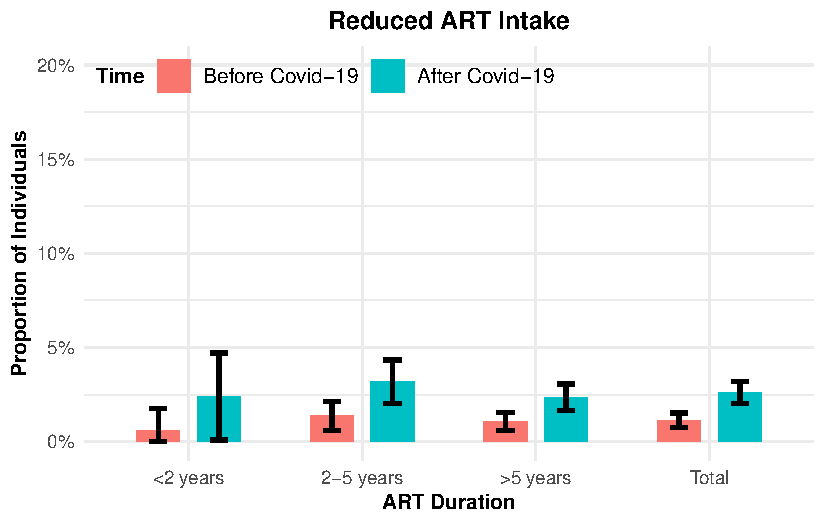
\includegraphics[keepaspectratio]{Rakai_revision_files/figure-pdf/unnamed-chunk-75-1.pdf}}

\subsubsection{Run out of ART by ART
Duration}\label{run-out-of-art-by-art-duration}

\begin{Shaded}
\begin{Highlighting}[]
\NormalTok{df\_dur }\SpecialCharTok{\%\textgreater{}\%} \FunctionTok{group\_by}\NormalTok{(art\_duration,artrunbc) }\SpecialCharTok{\%\textgreater{}\%} 
  \FunctionTok{count}\NormalTok{()}
\end{Highlighting}
\end{Shaded}

\begin{longtable}[]{@{}llr@{}}
\toprule\noalign{}
art\_duration & artrunbc & n \\
\midrule\noalign{}
\endhead
\bottomrule\noalign{}
\endlastfoot
\textless2 years & No & 165 \\
\textless2 years & Yes & 2 \\
2-5 years & No & 864 \\
2-5 years & Yes & 16 \\
\textgreater5 years & No & 1738 \\
\textgreater5 years & Yes & 49 \\
\end{longtable}

\begin{Shaded}
\begin{Highlighting}[]
\NormalTok{df\_dur }\SpecialCharTok{\%\textgreater{}\%} \FunctionTok{group\_by}\NormalTok{(art\_duration,artrunac) }\SpecialCharTok{\%\textgreater{}\%} 
  \FunctionTok{count}\NormalTok{()}
\end{Highlighting}
\end{Shaded}

\begin{longtable}[]{@{}llr@{}}
\toprule\noalign{}
art\_duration & artrunac & n \\
\midrule\noalign{}
\endhead
\bottomrule\noalign{}
\endlastfoot
\textless2 years & No & 157 \\
\textless2 years & Yes & 10 \\
2-5 years & No & 826 \\
2-5 years & Yes & 54 \\
\textgreater5 years & No & 1699 \\
\textgreater5 years & Yes & 88 \\
\end{longtable}

\begin{Shaded}
\begin{Highlighting}[]
\NormalTok{df\_dur\_artrun }\OtherTok{\textless{}{-}}\NormalTok{ df\_dur }\SpecialCharTok{\%\textgreater{}\%}
  \FunctionTok{mutate}\NormalTok{(}
    \AttributeTok{artrunbc =} \FunctionTok{as.character}\NormalTok{(artrunbc),}
    \AttributeTok{artrunac =} \FunctionTok{as.character}\NormalTok{(artrunac)}
\NormalTok{  ) }\SpecialCharTok{\%\textgreater{}\%}
  \FunctionTok{pivot\_longer}\NormalTok{(}
    \AttributeTok{cols =} \FunctionTok{c}\NormalTok{(artrunbc, artrunac),}
    \AttributeTok{names\_to =} \StringTok{"variable"}\NormalTok{,}
    \AttributeTok{values\_to =} \StringTok{"response"}
\NormalTok{  ) }\SpecialCharTok{\%\textgreater{}\%}
  \FunctionTok{mutate}\NormalTok{(}
    \AttributeTok{time =} \FunctionTok{if\_else}\NormalTok{(}\FunctionTok{grepl}\NormalTok{(}\StringTok{"bc$"}\NormalTok{, variable), }\StringTok{"Before Covid{-}19"}\NormalTok{, }\StringTok{"After Covid{-}19"}\NormalTok{)}
\NormalTok{  )}

\NormalTok{df\_dur\_artrun\_summary }\OtherTok{\textless{}{-}}\NormalTok{ df\_dur\_artrun }\SpecialCharTok{\%\textgreater{}\%}
  \FunctionTok{group\_by}\NormalTok{(time, art\_duration) }\SpecialCharTok{\%\textgreater{}\%}
  \FunctionTok{summarise}\NormalTok{(}
    \AttributeTok{n\_yes =} \FunctionTok{sum}\NormalTok{(response }\SpecialCharTok{==} \StringTok{"Yes"}\NormalTok{, }\AttributeTok{na.rm =} \ConstantTok{TRUE}\NormalTok{),}
    \AttributeTok{n =} \FunctionTok{n}\NormalTok{(),}
    \AttributeTok{.groups =} \StringTok{"drop"}
\NormalTok{  )}

\NormalTok{df\_dur\_artrun\_totals }\OtherTok{\textless{}{-}}\NormalTok{ df\_dur\_artrun }\SpecialCharTok{\%\textgreater{}\%}
  \FunctionTok{group\_by}\NormalTok{(time) }\SpecialCharTok{\%\textgreater{}\%}
  \FunctionTok{summarise}\NormalTok{(}
    \AttributeTok{n\_yes =} \FunctionTok{sum}\NormalTok{(response }\SpecialCharTok{==} \StringTok{"Yes"}\NormalTok{, }\AttributeTok{na.rm =} \ConstantTok{TRUE}\NormalTok{),}
    \AttributeTok{n =} \FunctionTok{n}\NormalTok{(),}
    \AttributeTok{.groups =} \StringTok{"drop"}
\NormalTok{  )}

\NormalTok{df\_dur\_artrun\_summary }\OtherTok{\textless{}{-}} \FunctionTok{bind\_rows}\NormalTok{(df\_dur\_artrun\_summary, df\_dur\_artrun\_totals) }\SpecialCharTok{\%\textgreater{}\%}
  \FunctionTok{mutate}\NormalTok{(}
    \AttributeTok{proportion =}\NormalTok{ n\_yes }\SpecialCharTok{/}\NormalTok{ n,}
    \AttributeTok{se =} \FunctionTok{sqrt}\NormalTok{(proportion }\SpecialCharTok{*}\NormalTok{ (}\DecValTok{1} \SpecialCharTok{{-}}\NormalTok{ proportion) }\SpecialCharTok{/}\NormalTok{ n),}
    \AttributeTok{lower =}\NormalTok{ proportion }\SpecialCharTok{{-}} \FloatTok{1.96} \SpecialCharTok{*}\NormalTok{ se,}
    \AttributeTok{upper =}\NormalTok{ proportion }\SpecialCharTok{+} \FloatTok{1.96} \SpecialCharTok{*}\NormalTok{ se}
\NormalTok{  ) }\SpecialCharTok{\%\textgreater{}\%} 
  \FunctionTok{mutate}\NormalTok{(}
    \AttributeTok{time =} \FunctionTok{as\_factor}\NormalTok{(time) }\SpecialCharTok{\%\textgreater{}\%} 
      \FunctionTok{fct\_relevel}\NormalTok{(}\StringTok{"Before Covid{-}19"}\NormalTok{),}
    \AttributeTok{art\_duration =} \FunctionTok{if\_else}\NormalTok{(}\FunctionTok{is.na}\NormalTok{(art\_duration), }\StringTok{"Total"}\NormalTok{, art\_duration)}\SpecialCharTok{\%\textgreater{}\%} 
      \FunctionTok{fct\_relevel}\NormalTok{(}\StringTok{"\textless{}2 years"}\NormalTok{,}\StringTok{"2{-}5 years"}\NormalTok{),}
    \AttributeTok{lower =} \FunctionTok{if\_else}\NormalTok{(lower }\SpecialCharTok{\textless{}} \DecValTok{0}\NormalTok{,}\DecValTok{0}\NormalTok{,lower)}
\NormalTok{  )}

\NormalTok{df\_dur\_artrun\_summary}
\end{Highlighting}
\end{Shaded}

\begin{longtable}[]{@{}
  >{\raggedright\arraybackslash}p{(\linewidth - 14\tabcolsep) * \real{0.1975}}
  >{\raggedright\arraybackslash}p{(\linewidth - 14\tabcolsep) * \real{0.1605}}
  >{\raggedleft\arraybackslash}p{(\linewidth - 14\tabcolsep) * \real{0.0741}}
  >{\raggedleft\arraybackslash}p{(\linewidth - 14\tabcolsep) * \real{0.0617}}
  >{\raggedleft\arraybackslash}p{(\linewidth - 14\tabcolsep) * \real{0.1358}}
  >{\raggedleft\arraybackslash}p{(\linewidth - 14\tabcolsep) * \real{0.1235}}
  >{\raggedleft\arraybackslash}p{(\linewidth - 14\tabcolsep) * \real{0.1235}}
  >{\raggedleft\arraybackslash}p{(\linewidth - 14\tabcolsep) * \real{0.1235}}@{}}
\toprule\noalign{}
\begin{minipage}[b]{\linewidth}\raggedright
time
\end{minipage} & \begin{minipage}[b]{\linewidth}\raggedright
art\_duration
\end{minipage} & \begin{minipage}[b]{\linewidth}\raggedleft
n\_yes
\end{minipage} & \begin{minipage}[b]{\linewidth}\raggedleft
n
\end{minipage} & \begin{minipage}[b]{\linewidth}\raggedleft
proportion
\end{minipage} & \begin{minipage}[b]{\linewidth}\raggedleft
se
\end{minipage} & \begin{minipage}[b]{\linewidth}\raggedleft
lower
\end{minipage} & \begin{minipage}[b]{\linewidth}\raggedleft
upper
\end{minipage} \\
\midrule\noalign{}
\endhead
\bottomrule\noalign{}
\endlastfoot
After Covid-19 & \textless2 years & 10 & 167 & 0.0598802 & 0.0183601 &
0.0238944 & 0.0958660 \\
After Covid-19 & 2-5 years & 54 & 880 & 0.0613636 & 0.0080903 &
0.0455067 & 0.0772206 \\
After Covid-19 & \textgreater5 years & 88 & 1787 & 0.0492445 & 0.0051186
& 0.0392121 & 0.0592770 \\
Before Covid-19 & \textless2 years & 2 & 167 & 0.0119760 & 0.0084175 &
0.0000000 & 0.0284743 \\
Before Covid-19 & 2-5 years & 16 & 880 & 0.0181818 & 0.0045039 &
0.0093541 & 0.0270095 \\
Before Covid-19 & \textgreater5 years & 49 & 1787 & 0.0274203 &
0.0038631 & 0.0198486 & 0.0349919 \\
After Covid-19 & Total & 152 & 2834 & 0.0536344 & 0.0042321 & 0.0453396
& 0.0619293 \\
Before Covid-19 & Total & 67 & 2834 & 0.0236415 & 0.0028539 & 0.0180478
& 0.0292352 \\
\end{longtable}

\begin{Shaded}
\begin{Highlighting}[]
\NormalTok{run\_out\_of\_art\_by\_duration\_plot }\OtherTok{\textless{}{-}} \FunctionTok{ggplot}\NormalTok{(df\_dur\_artrun\_summary, }\FunctionTok{aes}\NormalTok{(}\AttributeTok{x =}\NormalTok{ art\_duration, }\AttributeTok{y =}\NormalTok{ proportion, }\AttributeTok{fill =}\NormalTok{ time)) }\SpecialCharTok{+}
  \FunctionTok{geom\_col}\NormalTok{(}\AttributeTok{position =} \FunctionTok{position\_dodge}\NormalTok{(}\AttributeTok{width =} \FloatTok{0.7}\NormalTok{), }\AttributeTok{width =} \FloatTok{0.5}\NormalTok{) }\SpecialCharTok{+}
  \FunctionTok{geom\_errorbar}\NormalTok{(}
    \FunctionTok{aes}\NormalTok{(}\AttributeTok{ymin =}\NormalTok{ lower, }\AttributeTok{ymax =}\NormalTok{ upper),}
    \AttributeTok{position =} \FunctionTok{position\_dodge}\NormalTok{(}\AttributeTok{width =} \FloatTok{0.7}\NormalTok{),}
    \AttributeTok{width =} \FloatTok{0.2}\NormalTok{,}
    \AttributeTok{size =} \DecValTok{1}
\NormalTok{  ) }\SpecialCharTok{+}
  \FunctionTok{scale\_y\_continuous}\NormalTok{(}\AttributeTok{labels =}\NormalTok{ scales}\SpecialCharTok{::}\FunctionTok{percent\_format}\NormalTok{(}\AttributeTok{accuracy =} \DecValTok{1}\NormalTok{), }\AttributeTok{limits =} \FunctionTok{c}\NormalTok{(}\DecValTok{0}\NormalTok{, }\FloatTok{0.20}\NormalTok{)) }\SpecialCharTok{+}
  \FunctionTok{labs}\NormalTok{(}
    \AttributeTok{title =} \StringTok{"Run Out of ART"}\NormalTok{,}
    \AttributeTok{x =} \StringTok{"ART Duration"}\NormalTok{,}
    \AttributeTok{y =} \StringTok{"Proportion of individuals"}\NormalTok{,}
    \AttributeTok{fill =} \StringTok{"Time"}
\NormalTok{  ) }\SpecialCharTok{+}
  \FunctionTok{theme\_minimal}\NormalTok{() }\SpecialCharTok{+}
  \FunctionTok{theme}\NormalTok{(}
    \AttributeTok{plot.title =} \FunctionTok{element\_text}\NormalTok{(}\AttributeTok{hjust =} \FloatTok{0.5}\NormalTok{, }\AttributeTok{face =} \StringTok{"bold"}\NormalTok{, }\AttributeTok{size =} \DecValTok{12}\NormalTok{),}
    \AttributeTok{axis.title.x =} \FunctionTok{element\_text}\NormalTok{(}\AttributeTok{face =} \StringTok{"bold"}\NormalTok{, }\AttributeTok{size =} \DecValTok{10}\NormalTok{),}
    \AttributeTok{axis.title.y =} \FunctionTok{element\_text}\NormalTok{(}\AttributeTok{face =} \StringTok{"bold"}\NormalTok{, }\AttributeTok{size =} \DecValTok{10}\NormalTok{),}
    \AttributeTok{legend.title =} \FunctionTok{element\_text}\NormalTok{(}\AttributeTok{face =} \StringTok{"bold"}\NormalTok{, }\AttributeTok{size =} \DecValTok{10}\NormalTok{),}
    \AttributeTok{legend.text =} \FunctionTok{element\_text}\NormalTok{(}\AttributeTok{size =} \DecValTok{10}\NormalTok{),}
    \AttributeTok{legend.position =} \FunctionTok{c}\NormalTok{(}\DecValTok{0}\NormalTok{, }\DecValTok{1}\NormalTok{),}
    \AttributeTok{legend.justification =} \FunctionTok{c}\NormalTok{(}\DecValTok{0}\NormalTok{, }\DecValTok{1}\NormalTok{),}
    \AttributeTok{legend.direction =} \StringTok{"horizontal"}
\NormalTok{  )}

\NormalTok{run\_out\_of\_art\_by\_duration\_plot}
\end{Highlighting}
\end{Shaded}

\pandocbounded{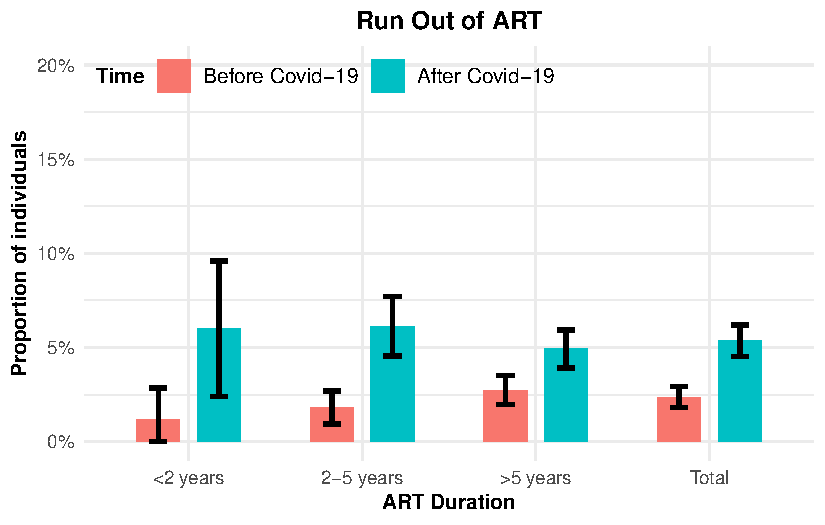
\includegraphics[keepaspectratio]{Rakai_revision_files/figure-pdf/unnamed-chunk-78-1.pdf}}

\subsubsection{Missed Scheduled visit by ART
Duration}\label{missed-scheduled-visit-by-art-duration}

\begin{Shaded}
\begin{Highlighting}[]
\NormalTok{df\_dur }\SpecialCharTok{\%\textgreater{}\%} \FunctionTok{group\_by}\NormalTok{(art\_duration,hivbc) }\SpecialCharTok{\%\textgreater{}\%} 
  \FunctionTok{count}\NormalTok{()}
\end{Highlighting}
\end{Shaded}

\begin{longtable}[]{@{}llr@{}}
\toprule\noalign{}
art\_duration & hivbc & n \\
\midrule\noalign{}
\endhead
\bottomrule\noalign{}
\endlastfoot
\textless2 years & No & 164 \\
\textless2 years & Yes & 3 \\
2-5 years & No & 849 \\
2-5 years & Yes & 31 \\
\textgreater5 years & No & 1726 \\
\textgreater5 years & Yes & 61 \\
\end{longtable}

\begin{Shaded}
\begin{Highlighting}[]
\NormalTok{df\_dur }\SpecialCharTok{\%\textgreater{}\%} \FunctionTok{group\_by}\NormalTok{(art\_duration,hivac) }\SpecialCharTok{\%\textgreater{}\%} 
  \FunctionTok{count}\NormalTok{()}
\end{Highlighting}
\end{Shaded}

\begin{longtable}[]{@{}llr@{}}
\toprule\noalign{}
art\_duration & hivac & n \\
\midrule\noalign{}
\endhead
\bottomrule\noalign{}
\endlastfoot
\textless2 years & No & 149 \\
\textless2 years & Yes & 18 \\
2-5 years & No & 788 \\
2-5 years & Yes & 92 \\
\textgreater5 years & No & 1622 \\
\textgreater5 years & Yes & 165 \\
\end{longtable}

\begin{Shaded}
\begin{Highlighting}[]
\NormalTok{df\_dur\_hiv }\OtherTok{\textless{}{-}}\NormalTok{ df\_dur }\SpecialCharTok{\%\textgreater{}\%}
  \FunctionTok{mutate}\NormalTok{(}
    \AttributeTok{hivbc =} \FunctionTok{as.character}\NormalTok{(hivbc),}
    \AttributeTok{hivac =} \FunctionTok{as.character}\NormalTok{(hivac)}
\NormalTok{  ) }\SpecialCharTok{\%\textgreater{}\%}
  \FunctionTok{pivot\_longer}\NormalTok{(}
    \AttributeTok{cols =} \FunctionTok{c}\NormalTok{(hivbc, hivac),}
    \AttributeTok{names\_to =} \StringTok{"variable"}\NormalTok{,}
    \AttributeTok{values\_to =} \StringTok{"response"}
\NormalTok{  ) }\SpecialCharTok{\%\textgreater{}\%}
  \FunctionTok{mutate}\NormalTok{(}
    \AttributeTok{time =} \FunctionTok{if\_else}\NormalTok{(}\FunctionTok{grepl}\NormalTok{(}\StringTok{"bc$"}\NormalTok{, variable), }\StringTok{"Before Covid{-}19"}\NormalTok{, }\StringTok{"After Covid{-}19"}\NormalTok{)}
\NormalTok{  )}

\NormalTok{df\_dur\_hiv\_summary }\OtherTok{\textless{}{-}}\NormalTok{ df\_dur\_hiv }\SpecialCharTok{\%\textgreater{}\%}
  \FunctionTok{group\_by}\NormalTok{(time, art\_duration) }\SpecialCharTok{\%\textgreater{}\%}
  \FunctionTok{summarise}\NormalTok{(}
    \AttributeTok{n\_yes =} \FunctionTok{sum}\NormalTok{(response }\SpecialCharTok{==} \StringTok{"Yes"}\NormalTok{, }\AttributeTok{na.rm =} \ConstantTok{TRUE}\NormalTok{),}
    \AttributeTok{n =} \FunctionTok{n}\NormalTok{(),}
    \AttributeTok{.groups =} \StringTok{"drop"}
\NormalTok{  )}

\NormalTok{df\_dur\_hiv\_totals }\OtherTok{\textless{}{-}}\NormalTok{ df\_dur\_hiv }\SpecialCharTok{\%\textgreater{}\%}
  \FunctionTok{group\_by}\NormalTok{(time) }\SpecialCharTok{\%\textgreater{}\%}
  \FunctionTok{summarise}\NormalTok{(}
    \AttributeTok{n\_yes =} \FunctionTok{sum}\NormalTok{(response }\SpecialCharTok{==} \StringTok{"Yes"}\NormalTok{, }\AttributeTok{na.rm =} \ConstantTok{TRUE}\NormalTok{),}
    \AttributeTok{n =} \FunctionTok{n}\NormalTok{(),}
    \AttributeTok{.groups =} \StringTok{"drop"}
\NormalTok{  ) }

\NormalTok{df\_dur\_hiv\_summary }\OtherTok{\textless{}{-}} \FunctionTok{bind\_rows}\NormalTok{(df\_dur\_hiv\_summary, df\_dur\_hiv\_totals) }\SpecialCharTok{\%\textgreater{}\%}
  \FunctionTok{mutate}\NormalTok{(}
    \AttributeTok{proportion =}\NormalTok{ n\_yes }\SpecialCharTok{/}\NormalTok{ n,}
    \AttributeTok{se =} \FunctionTok{sqrt}\NormalTok{(proportion }\SpecialCharTok{*}\NormalTok{ (}\DecValTok{1} \SpecialCharTok{{-}}\NormalTok{ proportion) }\SpecialCharTok{/}\NormalTok{ n),}
    \AttributeTok{lower =}\NormalTok{ proportion }\SpecialCharTok{{-}} \FloatTok{1.96} \SpecialCharTok{*}\NormalTok{ se,}
    \AttributeTok{upper =}\NormalTok{ proportion }\SpecialCharTok{+} \FloatTok{1.96} \SpecialCharTok{*}\NormalTok{ se}
\NormalTok{  ) }\SpecialCharTok{\%\textgreater{}\%} 
  \FunctionTok{mutate}\NormalTok{(}
    \AttributeTok{time =} \FunctionTok{as\_factor}\NormalTok{(time) }\SpecialCharTok{\%\textgreater{}\%} 
      \FunctionTok{fct\_relevel}\NormalTok{(}\StringTok{"Before Covid{-}19"}\NormalTok{),}
    \AttributeTok{art\_duration =} \FunctionTok{if\_else}\NormalTok{(}\FunctionTok{is.na}\NormalTok{(art\_duration), }\StringTok{"Total"}\NormalTok{, art\_duration)}\SpecialCharTok{\%\textgreater{}\%} 
      \FunctionTok{fct\_relevel}\NormalTok{(}\StringTok{"\textless{}2 years"}\NormalTok{,}\StringTok{"2{-}5 years"}\NormalTok{),}
    \AttributeTok{lower =} \FunctionTok{if\_else}\NormalTok{(lower }\SpecialCharTok{\textless{}} \DecValTok{0}\NormalTok{,}\DecValTok{0}\NormalTok{,lower)}
\NormalTok{  )}

\NormalTok{df\_dur\_hiv\_summary}
\end{Highlighting}
\end{Shaded}

\begin{longtable}[]{@{}
  >{\raggedright\arraybackslash}p{(\linewidth - 14\tabcolsep) * \real{0.1975}}
  >{\raggedright\arraybackslash}p{(\linewidth - 14\tabcolsep) * \real{0.1605}}
  >{\raggedleft\arraybackslash}p{(\linewidth - 14\tabcolsep) * \real{0.0741}}
  >{\raggedleft\arraybackslash}p{(\linewidth - 14\tabcolsep) * \real{0.0617}}
  >{\raggedleft\arraybackslash}p{(\linewidth - 14\tabcolsep) * \real{0.1358}}
  >{\raggedleft\arraybackslash}p{(\linewidth - 14\tabcolsep) * \real{0.1235}}
  >{\raggedleft\arraybackslash}p{(\linewidth - 14\tabcolsep) * \real{0.1235}}
  >{\raggedleft\arraybackslash}p{(\linewidth - 14\tabcolsep) * \real{0.1235}}@{}}
\toprule\noalign{}
\begin{minipage}[b]{\linewidth}\raggedright
time
\end{minipage} & \begin{minipage}[b]{\linewidth}\raggedright
art\_duration
\end{minipage} & \begin{minipage}[b]{\linewidth}\raggedleft
n\_yes
\end{minipage} & \begin{minipage}[b]{\linewidth}\raggedleft
n
\end{minipage} & \begin{minipage}[b]{\linewidth}\raggedleft
proportion
\end{minipage} & \begin{minipage}[b]{\linewidth}\raggedleft
se
\end{minipage} & \begin{minipage}[b]{\linewidth}\raggedleft
lower
\end{minipage} & \begin{minipage}[b]{\linewidth}\raggedleft
upper
\end{minipage} \\
\midrule\noalign{}
\endhead
\bottomrule\noalign{}
\endlastfoot
After Covid-19 & \textless2 years & 18 & 167 & 0.1077844 & 0.0239969 &
0.0607506 & 0.1548183 \\
After Covid-19 & 2-5 years & 92 & 880 & 0.1045455 & 0.0103141 &
0.0843297 & 0.1247612 \\
After Covid-19 & \textgreater5 years & 165 & 1787 & 0.0923335 &
0.0068483 & 0.0789109 & 0.1057561 \\
Before Covid-19 & \textless2 years & 3 & 167 & 0.0179641 & 0.0102780 &
0.0000000 & 0.0381089 \\
Before Covid-19 & 2-5 years & 31 & 880 & 0.0352273 & 0.0062146 &
0.0230467 & 0.0474078 \\
Before Covid-19 & \textgreater5 years & 61 & 1787 & 0.0341354 &
0.0042953 & 0.0257165 & 0.0425543 \\
After Covid-19 & Total & 275 & 2834 & 0.0970360 & 0.0055603 & 0.0861377
& 0.1079343 \\
Before Covid-19 & Total & 95 & 2834 & 0.0335215 & 0.0033811 & 0.0268946
& 0.0401485 \\
\end{longtable}

\begin{Shaded}
\begin{Highlighting}[]
\NormalTok{missed\_scheduled\_visit\_by\_duration\_plot }\OtherTok{\textless{}{-}} \FunctionTok{ggplot}\NormalTok{(df\_dur\_hiv\_summary, }\FunctionTok{aes}\NormalTok{(}\AttributeTok{x =}\NormalTok{ art\_duration, }\AttributeTok{y =}\NormalTok{ proportion, }\AttributeTok{fill =}\NormalTok{ time)) }\SpecialCharTok{+}
  \FunctionTok{geom\_col}\NormalTok{(}\AttributeTok{position =} \FunctionTok{position\_dodge}\NormalTok{(}\AttributeTok{width =} \FloatTok{0.7}\NormalTok{), }\AttributeTok{width =} \FloatTok{0.5}\NormalTok{) }\SpecialCharTok{+}
  \FunctionTok{geom\_errorbar}\NormalTok{(}
    \FunctionTok{aes}\NormalTok{(}\AttributeTok{ymin =}\NormalTok{ lower, }\AttributeTok{ymax =}\NormalTok{ upper),}
    \AttributeTok{position =} \FunctionTok{position\_dodge}\NormalTok{(}\AttributeTok{width =} \FloatTok{0.7}\NormalTok{),}
    \AttributeTok{width =} \FloatTok{0.2}\NormalTok{,}
    \AttributeTok{size =} \DecValTok{1}
\NormalTok{  ) }\SpecialCharTok{+}
  \FunctionTok{scale\_y\_continuous}\NormalTok{(}\AttributeTok{labels =}\NormalTok{ scales}\SpecialCharTok{::}\FunctionTok{percent\_format}\NormalTok{(}\AttributeTok{accuracy =} \DecValTok{1}\NormalTok{), }\AttributeTok{limits =} \FunctionTok{c}\NormalTok{(}\DecValTok{0}\NormalTok{, }\FloatTok{0.20}\NormalTok{)) }\SpecialCharTok{+}
  \FunctionTok{labs}\NormalTok{(}
    \AttributeTok{title =} \StringTok{"Missed Scheduled Visits"}\NormalTok{,}
    \AttributeTok{x =} \StringTok{"ART Duration"}\NormalTok{,}
    \AttributeTok{y =} \StringTok{"Proportion of individuals"}\NormalTok{,}
    \AttributeTok{fill =} \StringTok{"Time"}
\NormalTok{  ) }\SpecialCharTok{+}
  \FunctionTok{theme\_minimal}\NormalTok{() }\SpecialCharTok{+}
  \FunctionTok{theme}\NormalTok{(}
    \AttributeTok{plot.title =} \FunctionTok{element\_text}\NormalTok{(}\AttributeTok{hjust =} \FloatTok{0.5}\NormalTok{, }\AttributeTok{face =} \StringTok{"bold"}\NormalTok{, }\AttributeTok{size =} \DecValTok{12}\NormalTok{),}
    \AttributeTok{axis.title.x =} \FunctionTok{element\_text}\NormalTok{(}\AttributeTok{face =} \StringTok{"bold"}\NormalTok{, }\AttributeTok{size =} \DecValTok{10}\NormalTok{),}
    \AttributeTok{axis.title.y =} \FunctionTok{element\_text}\NormalTok{(}\AttributeTok{face =} \StringTok{"bold"}\NormalTok{, }\AttributeTok{size =} \DecValTok{10}\NormalTok{),}
    \AttributeTok{legend.title =} \FunctionTok{element\_text}\NormalTok{(}\AttributeTok{face =} \StringTok{"bold"}\NormalTok{, }\AttributeTok{size =} \DecValTok{10}\NormalTok{),}
    \AttributeTok{legend.text =} \FunctionTok{element\_text}\NormalTok{(}\AttributeTok{size =} \DecValTok{10}\NormalTok{),}
    \AttributeTok{legend.position =} \FunctionTok{c}\NormalTok{(}\DecValTok{0}\NormalTok{, }\DecValTok{1}\NormalTok{),}
    \AttributeTok{legend.justification =} \FunctionTok{c}\NormalTok{(}\DecValTok{0}\NormalTok{, }\DecValTok{1}\NormalTok{),}
    \AttributeTok{legend.direction =} \StringTok{"horizontal"}
\NormalTok{  )}

\NormalTok{missed\_scheduled\_visit\_by\_duration\_plot}
\end{Highlighting}
\end{Shaded}

\pandocbounded{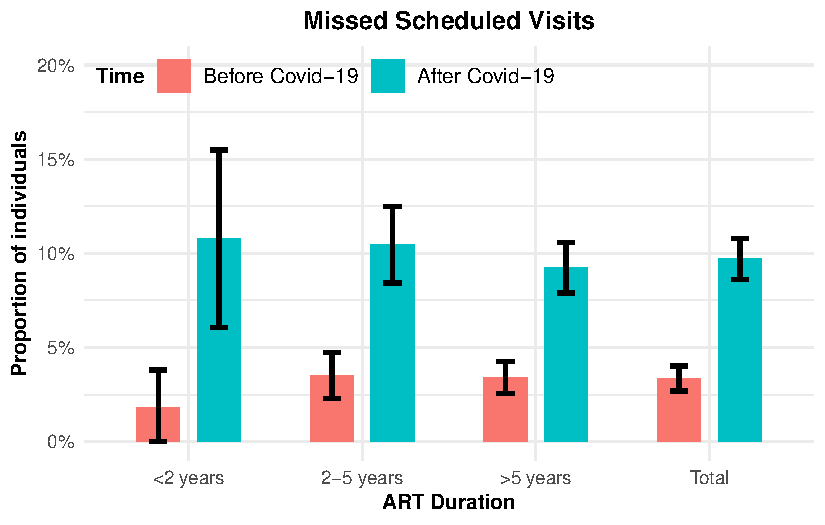
\includegraphics[keepaspectratio]{Rakai_revision_files/figure-pdf/unnamed-chunk-81-1.pdf}}

\begin{Shaded}
\begin{Highlighting}[]
\NormalTok{pd1 }\OtherTok{\textless{}{-}} \FunctionTok{ggplot}\NormalTok{(df\_dur\_artstr\_summary, }\FunctionTok{aes}\NormalTok{(}\AttributeTok{x =}\NormalTok{ art\_duration, }\AttributeTok{y =}\NormalTok{ proportion, }\AttributeTok{fill =}\NormalTok{ time)) }\SpecialCharTok{+}
  \FunctionTok{geom\_col}\NormalTok{(}\AttributeTok{position =} \FunctionTok{position\_dodge}\NormalTok{(}\AttributeTok{width =} \FloatTok{0.7}\NormalTok{), }\AttributeTok{width =} \FloatTok{0.5}\NormalTok{) }\SpecialCharTok{+}
  \FunctionTok{geom\_errorbar}\NormalTok{(}
    \FunctionTok{aes}\NormalTok{(}\AttributeTok{ymin =}\NormalTok{ lower, }\AttributeTok{ymax =}\NormalTok{ upper),}
    \AttributeTok{position =} \FunctionTok{position\_dodge}\NormalTok{(}\AttributeTok{width =} \FloatTok{0.7}\NormalTok{),}
    \AttributeTok{width =} \FloatTok{0.2}\NormalTok{,}
    \AttributeTok{size =} \DecValTok{1}
\NormalTok{  ) }\SpecialCharTok{+}
  \FunctionTok{scale\_y\_continuous}\NormalTok{(}\AttributeTok{labels =}\NormalTok{ scales}\SpecialCharTok{::}\FunctionTok{percent\_format}\NormalTok{(}\AttributeTok{accuracy =} \DecValTok{1}\NormalTok{), }\AttributeTok{limits =} \FunctionTok{c}\NormalTok{(}\DecValTok{0}\NormalTok{, }\FloatTok{0.25}\NormalTok{)) }\SpecialCharTok{+}
  \FunctionTok{labs}\NormalTok{(}
    \AttributeTok{title =} \StringTok{"Reduced ART Intake"}\NormalTok{,}
    \AttributeTok{x =} \StringTok{"ART Duration"}\NormalTok{,}
    \AttributeTok{y =} \StringTok{"Proportion of individuals"}\NormalTok{,}
    \AttributeTok{fill =} \StringTok{"Time"}
\NormalTok{  ) }\SpecialCharTok{+}
  \FunctionTok{theme\_minimal}\NormalTok{() }\SpecialCharTok{+}
  \FunctionTok{theme}\NormalTok{(}
    \AttributeTok{plot.title =} \FunctionTok{element\_text}\NormalTok{(}\AttributeTok{hjust =} \FloatTok{0.5}\NormalTok{, }\AttributeTok{face =} \StringTok{"bold"}\NormalTok{, }\AttributeTok{size =} \DecValTok{14}\NormalTok{),}
    \AttributeTok{axis.title.x =} \FunctionTok{element\_text}\NormalTok{(}\AttributeTok{face =} \StringTok{"bold"}\NormalTok{, }\AttributeTok{size =} \DecValTok{10}\NormalTok{),}
    \AttributeTok{axis.title.y =} \FunctionTok{element\_text}\NormalTok{(}\AttributeTok{face =} \StringTok{"bold"}\NormalTok{, }\AttributeTok{size =} \DecValTok{10}\NormalTok{),}
    \AttributeTok{legend.title =} \FunctionTok{element\_text}\NormalTok{(}\AttributeTok{face =} \StringTok{"bold"}\NormalTok{, }\AttributeTok{size =} \DecValTok{10}\NormalTok{),}
    \AttributeTok{legend.text =} \FunctionTok{element\_text}\NormalTok{(}\AttributeTok{size =} \DecValTok{10}\NormalTok{),}
    \AttributeTok{legend.position =} \FunctionTok{c}\NormalTok{(}\DecValTok{0}\NormalTok{, }\DecValTok{1}\NormalTok{), }
    \AttributeTok{legend.justification =} \FunctionTok{c}\NormalTok{(}\DecValTok{0}\NormalTok{, }\DecValTok{1}\NormalTok{),}
    \AttributeTok{legend.direction =} \StringTok{"horizontal"}
\NormalTok{  )}

\NormalTok{pd1}
\end{Highlighting}
\end{Shaded}

\pandocbounded{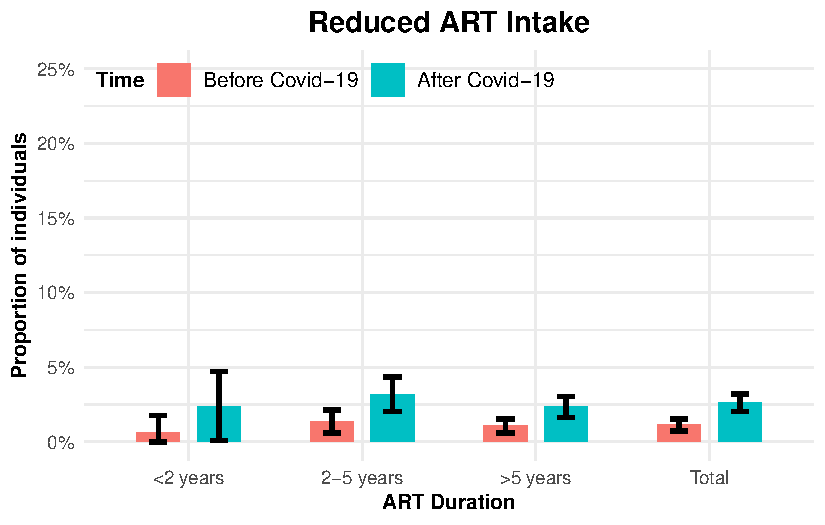
\includegraphics[keepaspectratio]{Rakai_revision_files/figure-pdf/unnamed-chunk-82-1.pdf}}

\begin{Shaded}
\begin{Highlighting}[]
\NormalTok{pd2 }\OtherTok{\textless{}{-}} \FunctionTok{ggplot}\NormalTok{(df\_dur\_hiv\_summary, }\FunctionTok{aes}\NormalTok{(}\AttributeTok{x =}\NormalTok{ art\_duration, }\AttributeTok{y =}\NormalTok{ proportion, }\AttributeTok{fill =}\NormalTok{ time)) }\SpecialCharTok{+}
  \FunctionTok{geom\_col}\NormalTok{(}\AttributeTok{position =} \FunctionTok{position\_dodge}\NormalTok{(}\AttributeTok{width =} \FloatTok{0.7}\NormalTok{), }\AttributeTok{width =} \FloatTok{0.5}\NormalTok{) }\SpecialCharTok{+}
  \FunctionTok{geom\_errorbar}\NormalTok{(}
    \FunctionTok{aes}\NormalTok{(}\AttributeTok{ymin =}\NormalTok{ lower, }\AttributeTok{ymax =}\NormalTok{ upper),}
    \AttributeTok{position =} \FunctionTok{position\_dodge}\NormalTok{(}\AttributeTok{width =} \FloatTok{0.7}\NormalTok{),}
    \AttributeTok{width =} \FloatTok{0.2}\NormalTok{,}
    \AttributeTok{size =} \DecValTok{1}
\NormalTok{  ) }\SpecialCharTok{+}
  \FunctionTok{scale\_y\_continuous}\NormalTok{(}\AttributeTok{labels =}\NormalTok{ scales}\SpecialCharTok{::}\FunctionTok{percent\_format}\NormalTok{(}\AttributeTok{accuracy =} \DecValTok{1}\NormalTok{), }\AttributeTok{limits =} \FunctionTok{c}\NormalTok{(}\DecValTok{0}\NormalTok{, }\FloatTok{0.25}\NormalTok{)) }\SpecialCharTok{+}
  \FunctionTok{labs}\NormalTok{(}
    \AttributeTok{title =} \StringTok{"Missed Scheduled Visits"}\NormalTok{,}
    \AttributeTok{x =} \StringTok{"ART Duration"}\NormalTok{,}
    \AttributeTok{y =} \StringTok{"Proportion of individuals"}\NormalTok{,}
    \AttributeTok{fill =} \StringTok{"Time"}
\NormalTok{  ) }\SpecialCharTok{+}
  \FunctionTok{theme\_minimal}\NormalTok{() }\SpecialCharTok{+}
  \FunctionTok{theme}\NormalTok{(}
    \AttributeTok{plot.title =} \FunctionTok{element\_text}\NormalTok{(}\AttributeTok{hjust =} \FloatTok{0.5}\NormalTok{, }\AttributeTok{face =} \StringTok{"bold"}\NormalTok{, }\AttributeTok{size =} \DecValTok{12}\NormalTok{),}
    \AttributeTok{axis.title.x =} \FunctionTok{element\_text}\NormalTok{(}\AttributeTok{face =} \StringTok{"bold"}\NormalTok{, }\AttributeTok{size =} \DecValTok{10}\NormalTok{),}
    \AttributeTok{axis.title.y =} \FunctionTok{element\_text}\NormalTok{(}\AttributeTok{face =} \StringTok{"bold"}\NormalTok{, }\AttributeTok{size =} \DecValTok{10}\NormalTok{),}
    \AttributeTok{legend.title =} \FunctionTok{element\_text}\NormalTok{(}\AttributeTok{face =} \StringTok{"bold"}\NormalTok{, }\AttributeTok{size =} \DecValTok{10}\NormalTok{),}
    \AttributeTok{legend.text =} \FunctionTok{element\_text}\NormalTok{(}\AttributeTok{size =} \DecValTok{10}\NormalTok{),}
    \AttributeTok{legend.position =} \FunctionTok{c}\NormalTok{(}\DecValTok{0}\NormalTok{, }\DecValTok{1}\NormalTok{), }
    \AttributeTok{legend.justification =} \FunctionTok{c}\NormalTok{(}\DecValTok{0}\NormalTok{, }\DecValTok{1}\NormalTok{),}
    \AttributeTok{legend.direction =} \StringTok{"horizontal"}
\NormalTok{  )}

\NormalTok{pd2}
\end{Highlighting}
\end{Shaded}

\pandocbounded{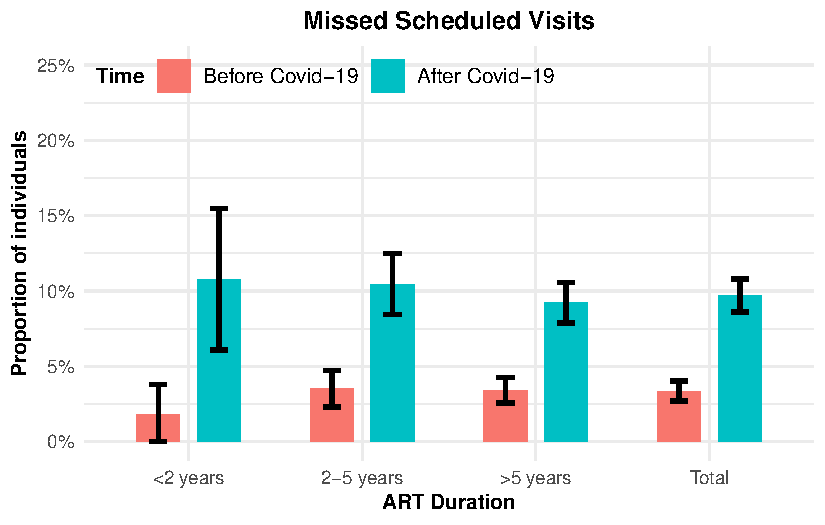
\includegraphics[keepaspectratio]{Rakai_revision_files/figure-pdf/unnamed-chunk-83-1.pdf}}

\begin{Shaded}
\begin{Highlighting}[]
\NormalTok{pd3 }\OtherTok{\textless{}{-}} \FunctionTok{ggplot}\NormalTok{(df\_dur\_artrun\_summary, }\FunctionTok{aes}\NormalTok{(}\AttributeTok{x =}\NormalTok{ art\_duration, }\AttributeTok{y =}\NormalTok{ proportion, }\AttributeTok{fill =}\NormalTok{ time)) }\SpecialCharTok{+}
  \FunctionTok{geom\_col}\NormalTok{(}\AttributeTok{position =} \FunctionTok{position\_dodge}\NormalTok{(}\AttributeTok{width =} \FloatTok{0.7}\NormalTok{), }\AttributeTok{width =} \FloatTok{0.5}\NormalTok{) }\SpecialCharTok{+}
  \FunctionTok{geom\_errorbar}\NormalTok{(}
    \FunctionTok{aes}\NormalTok{(}\AttributeTok{ymin =}\NormalTok{ lower, }\AttributeTok{ymax =}\NormalTok{ upper),}
    \AttributeTok{position =} \FunctionTok{position\_dodge}\NormalTok{(}\AttributeTok{width =} \FloatTok{0.7}\NormalTok{),}
    \AttributeTok{width =} \FloatTok{0.2}\NormalTok{,}
    \AttributeTok{size =} \DecValTok{1}
\NormalTok{  ) }\SpecialCharTok{+}
  \FunctionTok{scale\_y\_continuous}\NormalTok{(}\AttributeTok{labels =}\NormalTok{ scales}\SpecialCharTok{::}\FunctionTok{percent\_format}\NormalTok{(}\AttributeTok{accuracy =} \DecValTok{1}\NormalTok{), }\AttributeTok{limits =} \FunctionTok{c}\NormalTok{(}\DecValTok{0}\NormalTok{, }\FloatTok{0.25}\NormalTok{)) }\SpecialCharTok{+}
  \FunctionTok{labs}\NormalTok{(}
    \AttributeTok{title =} \StringTok{"Run Out of ART"}\NormalTok{,}
    \AttributeTok{x =} \StringTok{"ART Duration"}\NormalTok{,}
    \AttributeTok{y =} \StringTok{"Proportion of individuals"}\NormalTok{,}
    \AttributeTok{fill =} \StringTok{"Time"}
\NormalTok{  ) }\SpecialCharTok{+}
  \FunctionTok{theme\_minimal}\NormalTok{() }\SpecialCharTok{+}
  \FunctionTok{theme}\NormalTok{(}
    \AttributeTok{plot.title =} \FunctionTok{element\_text}\NormalTok{(}\AttributeTok{hjust =} \FloatTok{0.5}\NormalTok{, }\AttributeTok{face =} \StringTok{"bold"}\NormalTok{, }\AttributeTok{size =} \DecValTok{12}\NormalTok{),}
    \AttributeTok{axis.title.x =} \FunctionTok{element\_text}\NormalTok{(}\AttributeTok{face =} \StringTok{"bold"}\NormalTok{, }\AttributeTok{size =} \DecValTok{10}\NormalTok{),}
    \AttributeTok{axis.title.y =} \FunctionTok{element\_text}\NormalTok{(}\AttributeTok{face =} \StringTok{"bold"}\NormalTok{, }\AttributeTok{size =} \DecValTok{10}\NormalTok{),}
    \AttributeTok{legend.title =} \FunctionTok{element\_text}\NormalTok{(}\AttributeTok{face =} \StringTok{"bold"}\NormalTok{, }\AttributeTok{size =} \DecValTok{10}\NormalTok{),}
    \AttributeTok{legend.text =} \FunctionTok{element\_text}\NormalTok{(}\AttributeTok{size =} \DecValTok{10}\NormalTok{),}
    \AttributeTok{legend.position =} \FunctionTok{c}\NormalTok{(}\DecValTok{0}\NormalTok{, }\DecValTok{1}\NormalTok{), }
    \AttributeTok{legend.justification =} \FunctionTok{c}\NormalTok{(}\DecValTok{0}\NormalTok{, }\DecValTok{1}\NormalTok{),}
    \AttributeTok{legend.direction =} \StringTok{"horizontal"}
\NormalTok{  )}

\NormalTok{pd3}
\end{Highlighting}
\end{Shaded}

\pandocbounded{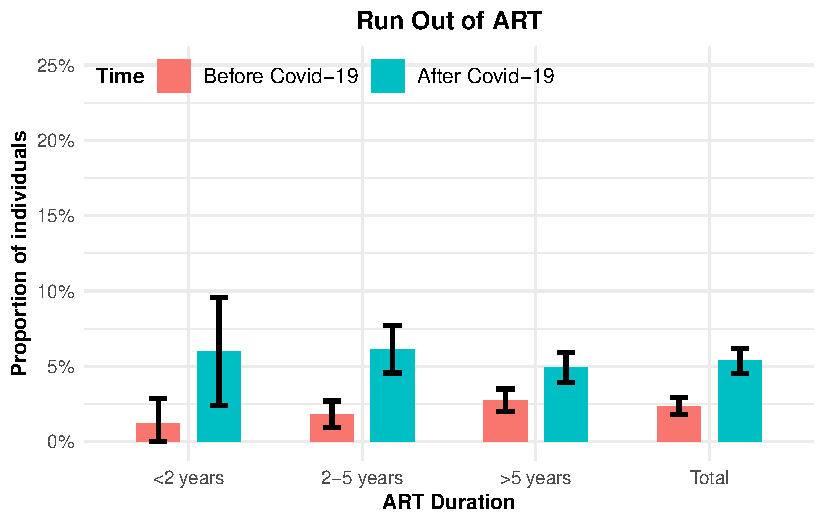
\includegraphics[keepaspectratio]{Rakai_revision_files/figure-pdf/unnamed-chunk-84-1.pdf}}

\begin{Shaded}
\begin{Highlighting}[]
\DocumentationTok{\#\#\# Combined plot}
\NormalTok{(pd1 }\SpecialCharTok{+}\NormalTok{ pd2)}\SpecialCharTok{/}\NormalTok{pd3}
\end{Highlighting}
\end{Shaded}

\pandocbounded{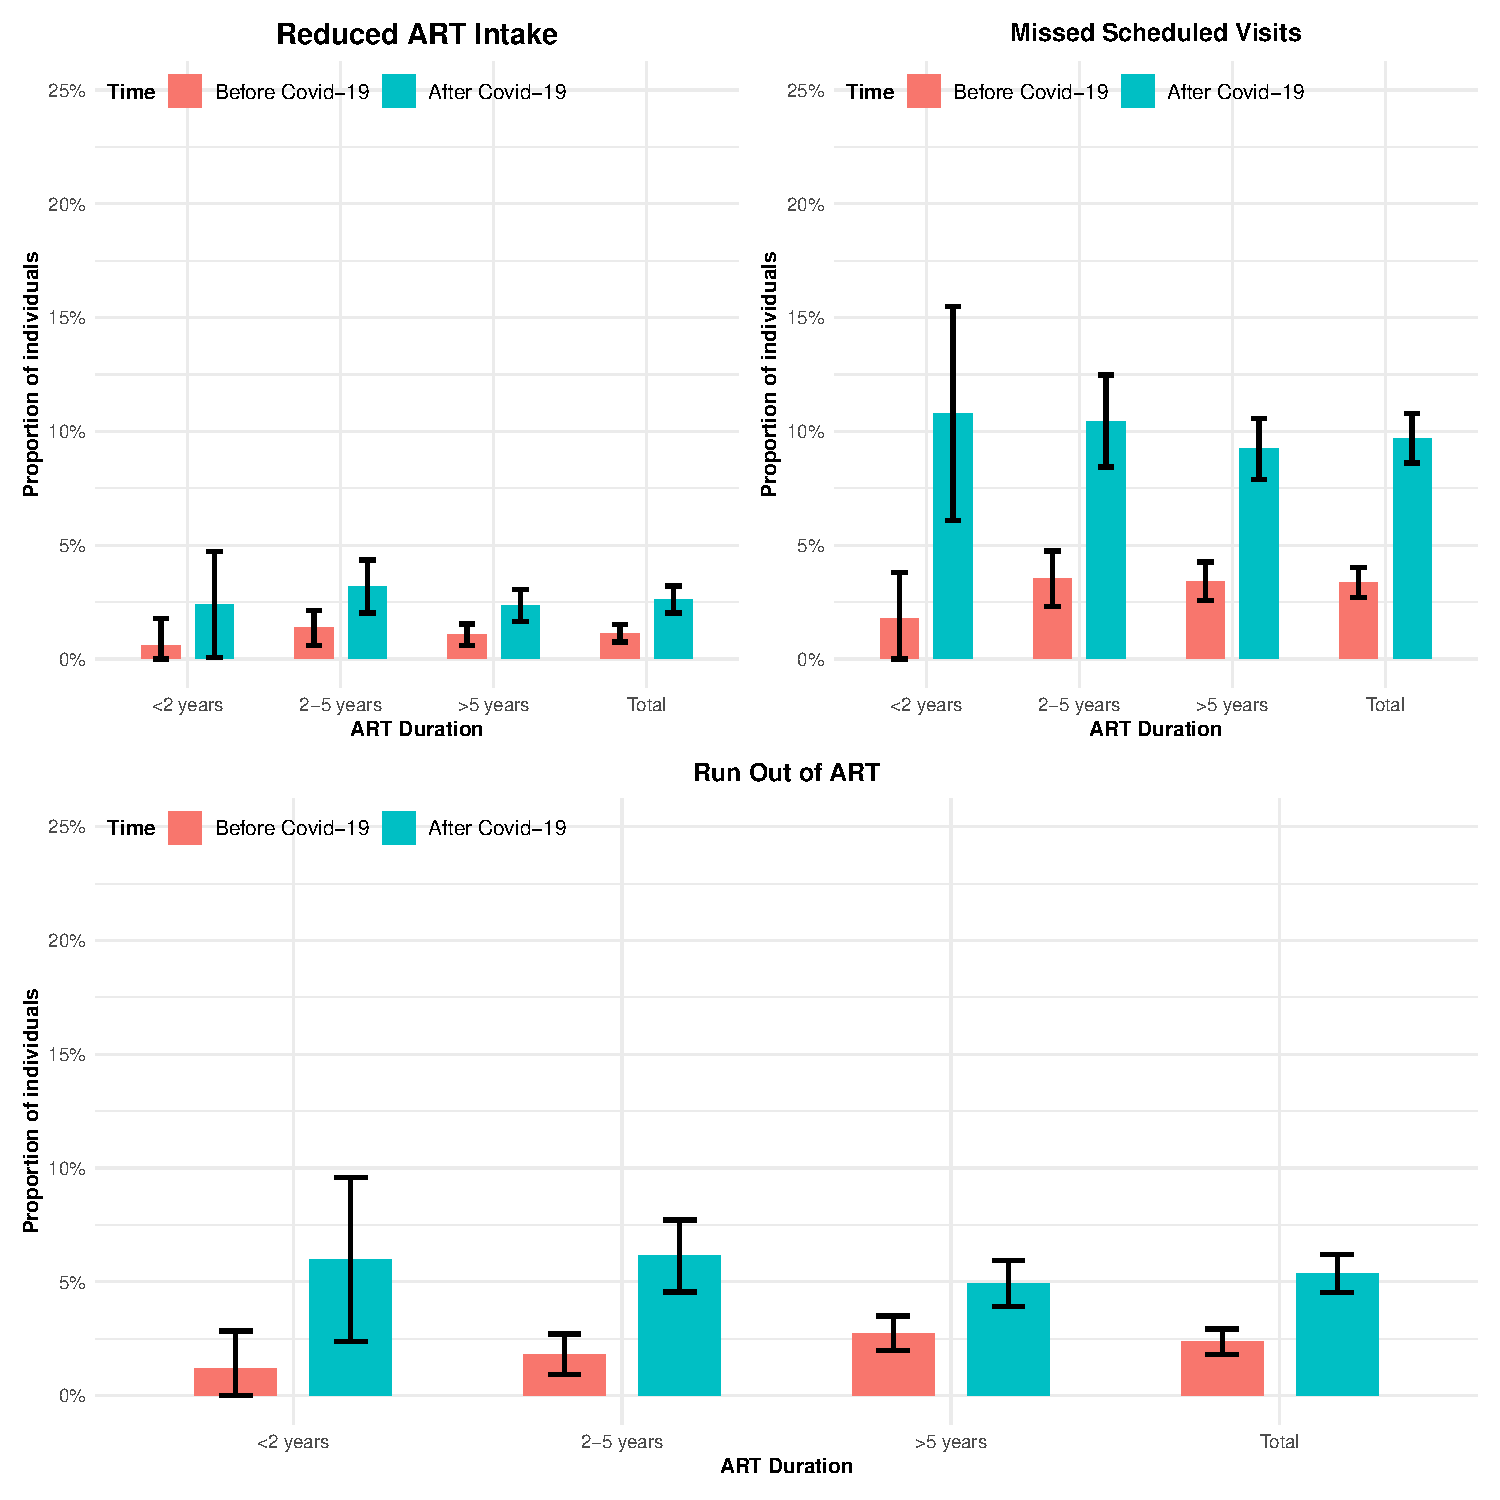
\includegraphics[keepaspectratio]{Rakai_revision_files/figure-pdf/unnamed-chunk-85-1.pdf}}

\section{Any disruption subplots}\label{any-disruption-subplots}

\begin{Shaded}
\begin{Highlighting}[]
\NormalTok{df\_disruption }\OtherTok{\textless{}{-}}\NormalTok{  rakai }\SpecialCharTok{\%\textgreater{}\%} 
   \FunctionTok{select}\NormalTok{(ageyrs,sex,mobility,arthoac,artrunac,artstrac,}
\NormalTok{    artyrs,comm\_num,artrunbc,artstrbc,hivac,hivbc,copies,new\_copies) }\SpecialCharTok{\%\textgreater{}\%} 
   \FunctionTok{mutate}\NormalTok{(}
     \AttributeTok{age\_cat =} \FunctionTok{case\_when}\NormalTok{(}
\NormalTok{       ageyrs }\SpecialCharTok{\textless{}} \DecValTok{30} \SpecialCharTok{\textasciitilde{}} \StringTok{"\textless{}30"}\NormalTok{,}
\NormalTok{       ageyrs }\SpecialCharTok{\textgreater{}=} \DecValTok{30} \SpecialCharTok{\&}\NormalTok{ ageyrs }\SpecialCharTok{\textless{}=} \DecValTok{39} \SpecialCharTok{\textasciitilde{}}  \StringTok{"30{-}39"}\NormalTok{,}
\NormalTok{       ageyrs }\SpecialCharTok{\textgreater{}=}\DecValTok{40} \SpecialCharTok{\&}\NormalTok{ ageyrs }\SpecialCharTok{\textless{}=} \DecValTok{49} \SpecialCharTok{\textasciitilde{}} \StringTok{"40{-}49"}\NormalTok{) }\SpecialCharTok{\%\textgreater{}\%} 
       \FunctionTok{fct\_relevel}\NormalTok{(}\StringTok{"\textless{}30"}\NormalTok{) }\SpecialCharTok{\%\textgreater{}\%} 
       \FunctionTok{ff\_label}\NormalTok{(}\StringTok{"Age group"}\NormalTok{),}
     
     \AttributeTok{sex =} \FunctionTok{if\_else}\NormalTok{(sex }\SpecialCharTok{==} \StringTok{"F"}\NormalTok{,}\StringTok{"Female"}\NormalTok{,}\StringTok{"Male"}\NormalTok{) }\SpecialCharTok{\%\textgreater{}\%} 
       \FunctionTok{as\_factor}\NormalTok{() }\SpecialCharTok{\%\textgreater{}\%}
       \FunctionTok{fct\_relevel}\NormalTok{(}\StringTok{"Female"}\NormalTok{) }\SpecialCharTok{\%\textgreater{}\%} 
       \FunctionTok{ff\_label}\NormalTok{(}\StringTok{"Sex"}\NormalTok{),}
     
     \AttributeTok{mobility =} \FunctionTok{case\_when}\NormalTok{(}
\NormalTok{       mobility }\SpecialCharTok{\%in\%} \FunctionTok{c}\NormalTok{(}\DecValTok{3}\NormalTok{,}\DecValTok{8}\NormalTok{,}\DecValTok{10}\NormalTok{) }\SpecialCharTok{\textasciitilde{}} \StringTok{"In{-}migrant"}\NormalTok{,}
       \AttributeTok{.default =} \StringTok{"Long{-}term resident"}\NormalTok{) }\SpecialCharTok{\%\textgreater{}\%} 
       \FunctionTok{fct\_relevel}\NormalTok{(}\StringTok{"In{-}migrant"}\NormalTok{) }\SpecialCharTok{\%\textgreater{}\%} 
       \FunctionTok{ff\_label}\NormalTok{(}\StringTok{"Migration"}\NormalTok{),}
     
     \AttributeTok{community\_type =} \FunctionTok{case\_when}\NormalTok{(}
\NormalTok{       comm\_num }\SpecialCharTok{\%in\%} \FunctionTok{c}\NormalTok{(}\DecValTok{38}\NormalTok{,}\DecValTok{770}\NormalTok{,}\DecValTok{771}\NormalTok{,}\DecValTok{774}\NormalTok{) }\SpecialCharTok{\textasciitilde{}} \StringTok{"Fishing community"}\NormalTok{,}
       \AttributeTok{.default =} \StringTok{"Inland Community"}\NormalTok{) }\SpecialCharTok{\%\textgreater{}\%} 
       \FunctionTok{fct\_relevel}\NormalTok{(}\StringTok{"Inland Community"}\NormalTok{) }\SpecialCharTok{\%\textgreater{}\%} 
       \FunctionTok{ff\_label}\NormalTok{(}\StringTok{"Community type"}\NormalTok{),}
     \AttributeTok{fishing\_comm =} \FunctionTok{if\_else}\NormalTok{(community\_type }\SpecialCharTok{==} \StringTok{"Fishing Community"}\NormalTok{,}\DecValTok{1}\NormalTok{,}\DecValTok{0}\NormalTok{) }\SpecialCharTok{\%\textgreater{}\%} 
       \FunctionTok{ff\_label}\NormalTok{(}\StringTok{"Lake Victoria Fishing Community"}\NormalTok{),}
     
     \AttributeTok{art\_duration =} \FunctionTok{case\_when}\NormalTok{(}
\NormalTok{       artyrs }\SpecialCharTok{\textgreater{}=} \DecValTok{2} \SpecialCharTok{\&}\NormalTok{  artyrs }\SpecialCharTok{\textless{}=} \DecValTok{5} \SpecialCharTok{\textasciitilde{}} \StringTok{"2{-}5 years"}\NormalTok{,}
\NormalTok{       artyrs }\SpecialCharTok{\textgreater{}} \DecValTok{5} \SpecialCharTok{\textasciitilde{}} \StringTok{"\textgreater{}5 years"}\NormalTok{,}
       \AttributeTok{.default =}  \StringTok{"\textless{}2 years"}
\NormalTok{     ) }\SpecialCharTok{\%\textgreater{}\%} 
       \FunctionTok{fct\_relevel}\NormalTok{(}\StringTok{"\textless{}2 years"}\NormalTok{,}\StringTok{"2{-}5 years"}\NormalTok{) }\SpecialCharTok{\%\textgreater{}\%} 
       \FunctionTok{ff\_label}\NormalTok{(}\StringTok{"Time on ART"}\NormalTok{),}
     
     \AttributeTok{hivac =} \FunctionTok{if\_else}\NormalTok{(hivac }\SpecialCharTok{==} \DecValTok{1}\NormalTok{, }\DecValTok{1}\NormalTok{, }\DecValTok{0}\NormalTok{) }\SpecialCharTok{\%\textgreater{}\%} 
       \FunctionTok{ff\_label}\NormalTok{(}\StringTok{"Missed scheduled visit for HIV care"}\NormalTok{),}
     
     \AttributeTok{hivbc =} \FunctionTok{if\_else}\NormalTok{(hivbc }\SpecialCharTok{==} \DecValTok{1}\NormalTok{, }\DecValTok{1}\NormalTok{, }\DecValTok{0}\NormalTok{) }\SpecialCharTok{\%\textgreater{}\%} 
       \FunctionTok{ff\_label}\NormalTok{(}\StringTok{"Missed scheduled visit for HIV care"}\NormalTok{),}
     
     \AttributeTok{artrunac =} \FunctionTok{if\_else}\NormalTok{(artrunac }\SpecialCharTok{==} \DecValTok{1}\NormalTok{, }\DecValTok{1}\NormalTok{, }\DecValTok{0}\NormalTok{) }\SpecialCharTok{\%\textgreater{}\%} 
       \FunctionTok{ff\_label}\NormalTok{(}\StringTok{"Run out of ART before next refill"}\NormalTok{),}
     
     \AttributeTok{artrunbc =} \FunctionTok{if\_else}\NormalTok{(artrunbc }\SpecialCharTok{==} \DecValTok{1}\NormalTok{, }\DecValTok{1}\NormalTok{, }\DecValTok{0}\NormalTok{) }\SpecialCharTok{\%\textgreater{}\%} 
       \FunctionTok{ff\_label}\NormalTok{(}\StringTok{"Run out of ART before next refill"}\NormalTok{),}
     
     \AttributeTok{artstrac =} \FunctionTok{if\_else}\NormalTok{(artstrac }\SpecialCharTok{==} \DecValTok{1}\NormalTok{, }\DecValTok{1}\NormalTok{, }\DecValTok{0}\NormalTok{) }\SpecialCharTok{\%\textgreater{}\%} 
       \FunctionTok{ff\_label}\NormalTok{(}\StringTok{"Taken ART pills less frequently / in smaller amounts to conserve supply"}\NormalTok{),}
     
     \AttributeTok{artstrbc =} \FunctionTok{if\_else}\NormalTok{(artstrbc }\SpecialCharTok{==} \DecValTok{1}\NormalTok{, }\DecValTok{1}\NormalTok{, }\DecValTok{0}\NormalTok{) }\SpecialCharTok{\%\textgreater{}\%} 
       \FunctionTok{ff\_label}\NormalTok{(}\StringTok{"Taken ART pills less frequently / in smaller amounts to conserve supply"}\NormalTok{),}
     
\NormalTok{    )}
\end{Highlighting}
\end{Shaded}

\begin{Shaded}
\begin{Highlighting}[]
\NormalTok{df\_disruption }\OtherTok{\textless{}{-}}\NormalTok{  df\_disruption }\SpecialCharTok{\%\textgreater{}\%} 
  \FunctionTok{select}\NormalTok{(sex,age\_cat,community\_type,art\_duration,mobility,hivac,artrunac,artstrac,hivbc,artstrbc,artrunbc)}
\end{Highlighting}
\end{Shaded}

\begin{Shaded}
\begin{Highlighting}[]
\NormalTok{df\_disruption }\OtherTok{\textless{}{-}}\NormalTok{  df\_disruption }\SpecialCharTok{\%\textgreater{}\%} 
\FunctionTok{mutate}\NormalTok{(}\AttributeTok{any\_disruption\_b4 =} \FunctionTok{if\_else}\NormalTok{(}\FunctionTok{rowSums}\NormalTok{(}\FunctionTok{across}\NormalTok{(hivbc}\SpecialCharTok{:}\NormalTok{artrunbc),}\AttributeTok{na.rm =} \ConstantTok{TRUE}\NormalTok{) }\SpecialCharTok{\textgreater{}} \DecValTok{0}\NormalTok{,}\DecValTok{1}\NormalTok{,}\DecValTok{0}\NormalTok{),}
\AttributeTok{any\_disruption\_after =} \FunctionTok{if\_else}\NormalTok{(}\FunctionTok{rowSums}\NormalTok{(}\FunctionTok{across}\NormalTok{(hivac}\SpecialCharTok{:}\NormalTok{artstrac),}\AttributeTok{na.rm =} \ConstantTok{TRUE}\NormalTok{) }\SpecialCharTok{\textgreater{}} \DecValTok{0}\NormalTok{,}\DecValTok{1}\NormalTok{,}\DecValTok{0}\NormalTok{))}
\end{Highlighting}
\end{Shaded}

\begin{Shaded}
\begin{Highlighting}[]
\FunctionTok{table}\NormalTok{(df\_disruption}\SpecialCharTok{$}\NormalTok{any\_disruption\_b4)}
\end{Highlighting}
\end{Shaded}

\begin{verbatim}

   0    1 
2699  140 
\end{verbatim}

\begin{Shaded}
\begin{Highlighting}[]
\FunctionTok{table}\NormalTok{(df\_disruption}\SpecialCharTok{$}\NormalTok{any\_disruption\_after)}
\end{Highlighting}
\end{Shaded}

\begin{verbatim}

   0    1 
2457  382 
\end{verbatim}

\begin{Shaded}
\begin{Highlighting}[]
\NormalTok{prepare\_data }\OtherTok{\textless{}{-}} \ControlFlowTok{function}\NormalTok{(data, group\_var) \{}
\NormalTok{  grouped\_data }\OtherTok{\textless{}{-}}\NormalTok{ data }\SpecialCharTok{\%\textgreater{}\%}
    \FunctionTok{group\_by}\NormalTok{(\{\{ group\_var \}\}) }\SpecialCharTok{\%\textgreater{}\%}
    \FunctionTok{summarise}\NormalTok{(}
      \AttributeTok{n\_b4 =} \FunctionTok{sum}\NormalTok{(any\_disruption\_b4, }\AttributeTok{na.rm =} \ConstantTok{TRUE}\NormalTok{),}
      \AttributeTok{total\_b4 =} \FunctionTok{n}\NormalTok{(),}
      \AttributeTok{n\_after =} \FunctionTok{sum}\NormalTok{(any\_disruption\_after, }\AttributeTok{na.rm =} \ConstantTok{TRUE}\NormalTok{),}
      \AttributeTok{total\_after =} \FunctionTok{n}\NormalTok{(),}
      \AttributeTok{.groups =} \StringTok{"drop"}
\NormalTok{    ) }\SpecialCharTok{\%\textgreater{}\%}
    \FunctionTok{mutate}\NormalTok{(}
      \AttributeTok{proportion\_b4 =}\NormalTok{ n\_b4 }\SpecialCharTok{/}\NormalTok{ total\_b4,}
      \AttributeTok{proportion\_after =}\NormalTok{ n\_after }\SpecialCharTok{/}\NormalTok{ total\_after,}
      \AttributeTok{se\_b4 =} \FunctionTok{sqrt}\NormalTok{(proportion\_b4 }\SpecialCharTok{*}\NormalTok{ (}\DecValTok{1} \SpecialCharTok{{-}}\NormalTok{ proportion\_b4) }\SpecialCharTok{/}\NormalTok{ total\_b4),}
      \AttributeTok{se\_after =} \FunctionTok{sqrt}\NormalTok{(proportion\_after }\SpecialCharTok{*}\NormalTok{ (}\DecValTok{1} \SpecialCharTok{{-}}\NormalTok{ proportion\_after) }\SpecialCharTok{/}\NormalTok{ total\_after),}
      \AttributeTok{lower\_b4 =}\NormalTok{ proportion\_b4 }\SpecialCharTok{{-}} \FloatTok{1.96} \SpecialCharTok{*}\NormalTok{ se\_b4,}
      \AttributeTok{upper\_b4 =}\NormalTok{ proportion\_b4 }\SpecialCharTok{+} \FloatTok{1.96} \SpecialCharTok{*}\NormalTok{ se\_b4,}
      \AttributeTok{lower\_after =}\NormalTok{ proportion\_after }\SpecialCharTok{{-}} \FloatTok{1.96} \SpecialCharTok{*}\NormalTok{ se\_after,}
      \AttributeTok{upper\_after =}\NormalTok{ proportion\_after }\SpecialCharTok{+} \FloatTok{1.96} \SpecialCharTok{*}\NormalTok{ se\_after}
\NormalTok{    ) }\SpecialCharTok{\%\textgreater{}\%}
    \FunctionTok{pivot\_longer}\NormalTok{(}
      \AttributeTok{cols =} \FunctionTok{starts\_with}\NormalTok{(}\StringTok{"proportion"}\NormalTok{),}
      \AttributeTok{names\_to =} \StringTok{"time"}\NormalTok{,}
      \AttributeTok{values\_to =} \StringTok{"proportion"}
\NormalTok{    ) }\SpecialCharTok{\%\textgreater{}\%}
    \FunctionTok{mutate}\NormalTok{(}
      \AttributeTok{time =} \FunctionTok{if\_else}\NormalTok{(time }\SpecialCharTok{==} \StringTok{"proportion\_b4"}\NormalTok{, }\StringTok{"Before Covid{-}19"}\NormalTok{, }\StringTok{"After Covid{-}19"}\NormalTok{),}
      \AttributeTok{lower =} \FunctionTok{if\_else}\NormalTok{(time }\SpecialCharTok{==} \StringTok{"Before Covid{-}19"}\NormalTok{, lower\_b4, lower\_after),}
      \AttributeTok{upper =} \FunctionTok{if\_else}\NormalTok{(time }\SpecialCharTok{==} \StringTok{"Before Covid{-}19"}\NormalTok{, upper\_b4, upper\_after)}
\NormalTok{    ) }\SpecialCharTok{\%\textgreater{}\%}
    \FunctionTok{select}\NormalTok{(\{\{ group\_var \}\}, time, proportion, lower, upper)}
  

\NormalTok{  total\_data }\OtherTok{\textless{}{-}}\NormalTok{ data }\SpecialCharTok{\%\textgreater{}\%}
    \FunctionTok{summarise}\NormalTok{(}
      \AttributeTok{n\_b4 =} \FunctionTok{sum}\NormalTok{(any\_disruption\_b4, }\AttributeTok{na.rm =} \ConstantTok{TRUE}\NormalTok{),}
      \AttributeTok{total\_b4 =} \FunctionTok{n}\NormalTok{(),}
      \AttributeTok{n\_after =} \FunctionTok{sum}\NormalTok{(any\_disruption\_after, }\AttributeTok{na.rm =} \ConstantTok{TRUE}\NormalTok{),}
      \AttributeTok{total\_after =} \FunctionTok{n}\NormalTok{(),}
      \AttributeTok{.groups =} \StringTok{"drop"}
\NormalTok{    ) }\SpecialCharTok{\%\textgreater{}\%}
    \FunctionTok{mutate}\NormalTok{(}
      \AttributeTok{proportion\_b4 =}\NormalTok{ n\_b4 }\SpecialCharTok{/}\NormalTok{ total\_b4,}
      \AttributeTok{proportion\_after =}\NormalTok{ n\_after }\SpecialCharTok{/}\NormalTok{ total\_after,}
      \AttributeTok{se\_b4 =} \FunctionTok{sqrt}\NormalTok{(proportion\_b4 }\SpecialCharTok{*}\NormalTok{ (}\DecValTok{1} \SpecialCharTok{{-}}\NormalTok{ proportion\_b4) }\SpecialCharTok{/}\NormalTok{ total\_b4),}
      \AttributeTok{se\_after =} \FunctionTok{sqrt}\NormalTok{(proportion\_after }\SpecialCharTok{*}\NormalTok{ (}\DecValTok{1} \SpecialCharTok{{-}}\NormalTok{ proportion\_after) }\SpecialCharTok{/}\NormalTok{ total\_after),}
      \AttributeTok{lower\_b4 =}\NormalTok{ proportion\_b4 }\SpecialCharTok{{-}} \FloatTok{1.96} \SpecialCharTok{*}\NormalTok{ se\_b4,}
      \AttributeTok{upper\_b4 =}\NormalTok{ proportion\_b4 }\SpecialCharTok{+} \FloatTok{1.96} \SpecialCharTok{*}\NormalTok{ se\_b4,}
      \AttributeTok{lower\_after =}\NormalTok{ proportion\_after }\SpecialCharTok{{-}} \FloatTok{1.96} \SpecialCharTok{*}\NormalTok{ se\_after,}
      \AttributeTok{upper\_after =}\NormalTok{ proportion\_after }\SpecialCharTok{+} \FloatTok{1.96} \SpecialCharTok{*}\NormalTok{ se\_after}
\NormalTok{    ) }\SpecialCharTok{\%\textgreater{}\%}
    \FunctionTok{pivot\_longer}\NormalTok{(}
      \AttributeTok{cols =} \FunctionTok{starts\_with}\NormalTok{(}\StringTok{"proportion"}\NormalTok{),}
      \AttributeTok{names\_to =} \StringTok{"time"}\NormalTok{,}
      \AttributeTok{values\_to =} \StringTok{"proportion"}
\NormalTok{    ) }\SpecialCharTok{\%\textgreater{}\%}
    \FunctionTok{mutate}\NormalTok{(}
      \AttributeTok{time =} \FunctionTok{if\_else}\NormalTok{(time }\SpecialCharTok{==} \StringTok{"proportion\_b4"}\NormalTok{, }\StringTok{"Before Covid{-}19"}\NormalTok{, }\StringTok{"After Covid{-}19"}\NormalTok{),}
      \AttributeTok{lower =} \FunctionTok{if\_else}\NormalTok{(time }\SpecialCharTok{==} \StringTok{"Before Covid{-}19"}\NormalTok{, lower\_b4, lower\_after),}
      \AttributeTok{upper =} \FunctionTok{if\_else}\NormalTok{(time }\SpecialCharTok{==} \StringTok{"Before Covid{-}19"}\NormalTok{, upper\_b4, upper\_after),}
\NormalTok{      \{\{ group\_var \}\} }\SpecialCharTok{:}\ErrorTok{=} \StringTok{"Total"} \CommentTok{\# Add "Total" to the group variable}
\NormalTok{    ) }\SpecialCharTok{\%\textgreater{}\%}
    \FunctionTok{select}\NormalTok{(\{\{ group\_var \}\}, time, proportion, lower, upper)}

  \FunctionTok{bind\_rows}\NormalTok{(grouped\_data, total\_data)}
\NormalTok{\}}
\end{Highlighting}
\end{Shaded}

\begin{Shaded}
\begin{Highlighting}[]
\NormalTok{summary\_by\_sex }\OtherTok{\textless{}{-}} \FunctionTok{prepare\_data}\NormalTok{(df\_disruption, sex)}
\NormalTok{summary\_by\_age }\OtherTok{\textless{}{-}} \FunctionTok{prepare\_data}\NormalTok{(df\_disruption, age\_cat)}
\NormalTok{summary\_by\_mobility }\OtherTok{\textless{}{-}} \FunctionTok{prepare\_data}\NormalTok{(df\_disruption, mobility)}
\NormalTok{summary\_by\_community }\OtherTok{\textless{}{-}} \FunctionTok{prepare\_data}\NormalTok{(df\_disruption, community\_type)}
\NormalTok{summary\_by\_art\_duration }\OtherTok{\textless{}{-}} \FunctionTok{prepare\_data}\NormalTok{(df\_disruption,art\_duration)}
\end{Highlighting}
\end{Shaded}

\begin{Shaded}
\begin{Highlighting}[]
\NormalTok{summary\_by\_age }\OtherTok{\textless{}{-}}\NormalTok{  summary\_by\_age }\SpecialCharTok{\%\textgreater{}\%} 
  \FunctionTok{mutate}\NormalTok{(}\AttributeTok{age\_cat =} \FunctionTok{as\_factor}\NormalTok{(age\_cat) }\SpecialCharTok{\%\textgreater{}\%} 
           \FunctionTok{fct\_relevel}\NormalTok{(}\StringTok{"\textless{}30"}\NormalTok{,}\StringTok{"30{-}39"}\NormalTok{,}\StringTok{"40{-}49"}\NormalTok{),}
         \AttributeTok{time =} \FunctionTok{as\_factor}\NormalTok{(time) }\SpecialCharTok{\%\textgreater{}\%} 
           \FunctionTok{fct\_relevel}\NormalTok{(}\StringTok{"Before Covid{-}19"}\NormalTok{))}
\end{Highlighting}
\end{Shaded}

\begin{Shaded}
\begin{Highlighting}[]
\NormalTok{summary\_by\_community }\OtherTok{\textless{}{-}}\NormalTok{  summary\_by\_community }\SpecialCharTok{\%\textgreater{}\%} 
  \FunctionTok{mutate}\NormalTok{(}
   \AttributeTok{time =} \FunctionTok{as\_factor}\NormalTok{(time) }\SpecialCharTok{\%\textgreater{}\%} 
           \FunctionTok{fct\_relevel}\NormalTok{(}\StringTok{"Before Covid{-}19"}\NormalTok{),}
   \AttributeTok{community\_type =} \FunctionTok{as\_factor}\NormalTok{(community\_type) }\SpecialCharTok{\%\textgreater{}\%} 
     \FunctionTok{fct\_relevel}\NormalTok{(}\StringTok{"Fishing community"}\NormalTok{)}
\NormalTok{  )}
\end{Highlighting}
\end{Shaded}

\begin{Shaded}
\begin{Highlighting}[]
\NormalTok{summary\_by\_mobility }\OtherTok{\textless{}{-}}\NormalTok{  summary\_by\_mobility }\SpecialCharTok{\%\textgreater{}\%} 
  \FunctionTok{mutate}\NormalTok{(}
    \AttributeTok{time =} \FunctionTok{as\_factor}\NormalTok{(time) }\SpecialCharTok{\%\textgreater{}\%} 
           \FunctionTok{fct\_relevel}\NormalTok{(}\StringTok{"Before Covid{-}19"}\NormalTok{),}
    \AttributeTok{mobility =} \FunctionTok{as\_factor}\NormalTok{(mobility) }\SpecialCharTok{\%\textgreater{}\%} 
      \FunctionTok{fct\_relevel}\NormalTok{(}\StringTok{"In{-}migrant"}\NormalTok{,}\StringTok{"Long{-}term resident"}\NormalTok{)}
\NormalTok{  )}
\end{Highlighting}
\end{Shaded}

\begin{Shaded}
\begin{Highlighting}[]
\NormalTok{summary\_by\_sex }\OtherTok{\textless{}{-}}\NormalTok{  summary\_by\_sex }\SpecialCharTok{\%\textgreater{}\%} 
  \FunctionTok{mutate}\NormalTok{(}
    \AttributeTok{time =} \FunctionTok{as\_factor}\NormalTok{(time) }\SpecialCharTok{\%\textgreater{}\%} 
           \FunctionTok{fct\_relevel}\NormalTok{(}\StringTok{"Before Covid{-}19"}\NormalTok{),}
    \AttributeTok{sex =} \FunctionTok{as\_factor}\NormalTok{(sex) }\SpecialCharTok{\%\textgreater{}\%} 
      \FunctionTok{fct\_relevel}\NormalTok{(}\StringTok{"Female"}\NormalTok{,}\StringTok{"Male"}\NormalTok{)}
\NormalTok{  )}
\end{Highlighting}
\end{Shaded}

\begin{Shaded}
\begin{Highlighting}[]
\NormalTok{summary\_by\_art\_duration }\OtherTok{\textless{}{-}}\NormalTok{  summary\_by\_art\_duration }\SpecialCharTok{\%\textgreater{}\%} 
  \FunctionTok{mutate}\NormalTok{(}
    \AttributeTok{time =} \FunctionTok{as\_factor}\NormalTok{(time) }\SpecialCharTok{\%\textgreater{}\%} 
           \FunctionTok{fct\_relevel}\NormalTok{(}\StringTok{"Before Covid{-}19"}\NormalTok{),}
    \AttributeTok{art\_duration =} \FunctionTok{as\_factor}\NormalTok{(art\_duration) }\SpecialCharTok{\%\textgreater{}\%} 
      \FunctionTok{fct\_relevel}\NormalTok{(}\StringTok{"\textless{}2 years"}\NormalTok{,}\StringTok{"2{-}5 years"}\NormalTok{, }\StringTok{"\textgreater{}5 years"}\NormalTok{,}\StringTok{"Total"}\NormalTok{)}
\NormalTok{  )}
\end{Highlighting}
\end{Shaded}

\subsubsection{Any Disruption by Sex}\label{any-disruption-by-sex}

\begin{Shaded}
\begin{Highlighting}[]
\NormalTok{pr1 }\OtherTok{\textless{}{-}}\NormalTok{ summary\_by\_sex }\SpecialCharTok{\%\textgreater{}\%} 
\FunctionTok{ggplot}\NormalTok{(}\FunctionTok{aes}\NormalTok{(}\AttributeTok{x =}\NormalTok{ sex, }\AttributeTok{y =}\NormalTok{ proportion, }\AttributeTok{fill =}\NormalTok{ time)) }\SpecialCharTok{+}
  \FunctionTok{geom\_col}\NormalTok{(}\AttributeTok{position =} \FunctionTok{position\_dodge}\NormalTok{(}\AttributeTok{width =} \FloatTok{0.7}\NormalTok{), }\AttributeTok{width =} \FloatTok{0.5}\NormalTok{) }\SpecialCharTok{+}
  \FunctionTok{geom\_errorbar}\NormalTok{(}
    \FunctionTok{aes}\NormalTok{(}\AttributeTok{ymin =}\NormalTok{ lower, }\AttributeTok{ymax =}\NormalTok{ upper),}
    \AttributeTok{position =} \FunctionTok{position\_dodge}\NormalTok{(}\AttributeTok{width =} \FloatTok{0.7}\NormalTok{),}
    \AttributeTok{width =} \FloatTok{0.2}\NormalTok{,}
    \AttributeTok{size =} \DecValTok{1}
\NormalTok{  ) }\SpecialCharTok{+}
  \FunctionTok{scale\_y\_continuous}\NormalTok{(}\AttributeTok{labels =}\NormalTok{ scales}\SpecialCharTok{::}\FunctionTok{percent\_format}\NormalTok{(}\AttributeTok{accuracy =} \DecValTok{1}\NormalTok{), }\AttributeTok{limits =} \FunctionTok{c}\NormalTok{(}\DecValTok{0}\NormalTok{, }\FloatTok{0.20}\NormalTok{)) }\SpecialCharTok{+}
  \FunctionTok{labs}\NormalTok{(}
    \AttributeTok{title =} \StringTok{"Any Disruption"}\NormalTok{,}
    \AttributeTok{x =} \StringTok{"Sex"}\NormalTok{,}
    \AttributeTok{y =} \StringTok{"Proportion of individuals"}\NormalTok{,}
    \AttributeTok{fill =} \StringTok{"Time"}
\NormalTok{  ) }\SpecialCharTok{+}
  \FunctionTok{theme\_minimal}\NormalTok{() }\SpecialCharTok{+}
  \FunctionTok{theme}\NormalTok{(}
    \AttributeTok{plot.title =} \FunctionTok{element\_text}\NormalTok{(}\AttributeTok{hjust =} \FloatTok{0.5}\NormalTok{, }\AttributeTok{face =} \StringTok{"bold"}\NormalTok{, }\AttributeTok{size =} \DecValTok{12}\NormalTok{),}
    \AttributeTok{axis.title.x =} \FunctionTok{element\_text}\NormalTok{(}\AttributeTok{face =} \StringTok{"bold"}\NormalTok{, }\AttributeTok{size =} \DecValTok{10}\NormalTok{),}
    \AttributeTok{axis.title.y =} \FunctionTok{element\_text}\NormalTok{(}\AttributeTok{face =} \StringTok{"bold"}\NormalTok{, }\AttributeTok{size =} \DecValTok{10}\NormalTok{),}
    \AttributeTok{legend.title =} \FunctionTok{element\_text}\NormalTok{(}\AttributeTok{face =} \StringTok{"bold"}\NormalTok{, }\AttributeTok{size =} \DecValTok{10}\NormalTok{),}
    \AttributeTok{legend.text =} \FunctionTok{element\_text}\NormalTok{(}\AttributeTok{size =} \DecValTok{10}\NormalTok{),}
    \AttributeTok{legend.position =} \FunctionTok{c}\NormalTok{(}\DecValTok{0}\NormalTok{, }\DecValTok{1}\NormalTok{), }
    \AttributeTok{legend.justification =} \FunctionTok{c}\NormalTok{(}\DecValTok{0}\NormalTok{, }\DecValTok{1}\NormalTok{),}
    \AttributeTok{legend.direction =} \StringTok{"horizontal"}
\NormalTok{  )}

\NormalTok{pr1}
\end{Highlighting}
\end{Shaded}

\pandocbounded{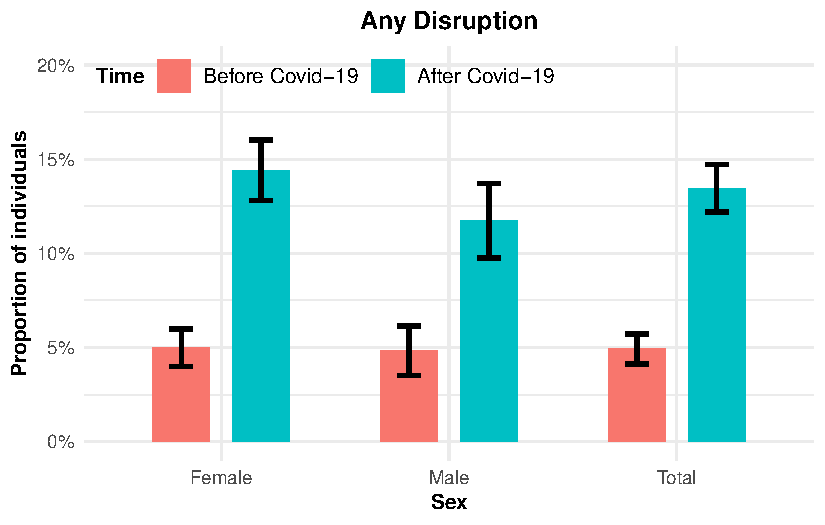
\includegraphics[keepaspectratio]{Rakai_revision_files/figure-pdf/unnamed-chunk-97-1.pdf}}

\subsubsection{Any disruption by community
type}\label{any-disruption-by-community-type}

\begin{Shaded}
\begin{Highlighting}[]
\NormalTok{pr2 }\OtherTok{\textless{}{-}}\NormalTok{ summary\_by\_community }\SpecialCharTok{\%\textgreater{}\%} 
\FunctionTok{ggplot}\NormalTok{(}\FunctionTok{aes}\NormalTok{(}\AttributeTok{x =}\NormalTok{ community\_type, }\AttributeTok{y =}\NormalTok{ proportion, }\AttributeTok{fill =}\NormalTok{ time)) }\SpecialCharTok{+}
  \FunctionTok{geom\_col}\NormalTok{(}\AttributeTok{position =} \FunctionTok{position\_dodge}\NormalTok{(}\AttributeTok{width =} \FloatTok{0.7}\NormalTok{), }\AttributeTok{width =} \FloatTok{0.5}\NormalTok{) }\SpecialCharTok{+}
  \FunctionTok{geom\_errorbar}\NormalTok{(}
    \FunctionTok{aes}\NormalTok{(}\AttributeTok{ymin =}\NormalTok{ lower, }\AttributeTok{ymax =}\NormalTok{ upper),}
    \AttributeTok{position =} \FunctionTok{position\_dodge}\NormalTok{(}\AttributeTok{width =} \FloatTok{0.7}\NormalTok{),}
    \AttributeTok{width =} \FloatTok{0.2}\NormalTok{,}
    \AttributeTok{size =} \DecValTok{1}
\NormalTok{  ) }\SpecialCharTok{+}
  \FunctionTok{scale\_y\_continuous}\NormalTok{(}\AttributeTok{labels =}\NormalTok{ scales}\SpecialCharTok{::}\FunctionTok{percent\_format}\NormalTok{(}\AttributeTok{accuracy =} \DecValTok{1}\NormalTok{), }\AttributeTok{limits =} \FunctionTok{c}\NormalTok{(}\DecValTok{0}\NormalTok{, }\FloatTok{0.25}\NormalTok{)) }\SpecialCharTok{+}
  \FunctionTok{labs}\NormalTok{(}
    \AttributeTok{title =} \StringTok{"Any Disruption"}\NormalTok{,}
    \AttributeTok{x =} \StringTok{"Community Type"}\NormalTok{,}
    \AttributeTok{y =} \StringTok{"Proportion of individuals"}\NormalTok{,}
    \AttributeTok{fill =} \StringTok{"Time"}
\NormalTok{  ) }\SpecialCharTok{+}
  \FunctionTok{theme\_minimal}\NormalTok{() }\SpecialCharTok{+}
  \FunctionTok{theme}\NormalTok{(}
    \AttributeTok{plot.title =} \FunctionTok{element\_text}\NormalTok{(}\AttributeTok{hjust =} \FloatTok{0.5}\NormalTok{, }\AttributeTok{face =} \StringTok{"bold"}\NormalTok{, }\AttributeTok{size =} \DecValTok{12}\NormalTok{),}
    \AttributeTok{axis.title.x =} \FunctionTok{element\_text}\NormalTok{(}\AttributeTok{face =} \StringTok{"bold"}\NormalTok{, }\AttributeTok{size =} \DecValTok{10}\NormalTok{),}
    \AttributeTok{axis.title.y =} \FunctionTok{element\_text}\NormalTok{(}\AttributeTok{face =} \StringTok{"bold"}\NormalTok{, }\AttributeTok{size =} \DecValTok{10}\NormalTok{),}
    \AttributeTok{legend.title =} \FunctionTok{element\_text}\NormalTok{(}\AttributeTok{face =} \StringTok{"bold"}\NormalTok{, }\AttributeTok{size =} \DecValTok{10}\NormalTok{),}
    \AttributeTok{legend.text =} \FunctionTok{element\_text}\NormalTok{(}\AttributeTok{size =} \DecValTok{10}\NormalTok{),}
    \AttributeTok{legend.position =} \FunctionTok{c}\NormalTok{(}\DecValTok{0}\NormalTok{, }\DecValTok{1}\NormalTok{), }
    \AttributeTok{legend.justification =} \FunctionTok{c}\NormalTok{(}\DecValTok{0}\NormalTok{, }\DecValTok{1}\NormalTok{),}
    \AttributeTok{legend.direction =} \StringTok{"horizontal"}
\NormalTok{  )}

\NormalTok{pr2}
\end{Highlighting}
\end{Shaded}

\pandocbounded{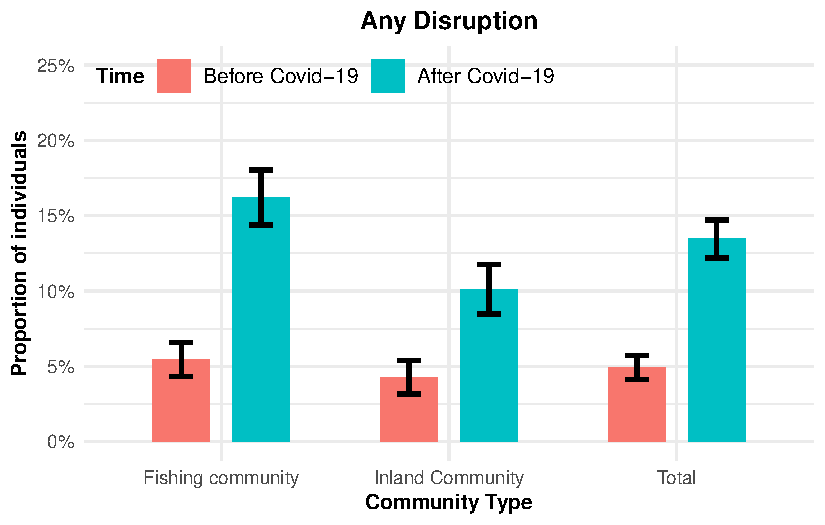
\includegraphics[keepaspectratio]{Rakai_revision_files/figure-pdf/unnamed-chunk-98-1.pdf}}

\subsubsection{Any disruption by age
category}\label{any-disruption-by-age-category}

\begin{Shaded}
\begin{Highlighting}[]
\NormalTok{pr3 }\OtherTok{\textless{}{-}}\NormalTok{ summary\_by\_age }\SpecialCharTok{\%\textgreater{}\%} 
\FunctionTok{ggplot}\NormalTok{(}\FunctionTok{aes}\NormalTok{(}\AttributeTok{x =}\NormalTok{ age\_cat, }\AttributeTok{y =}\NormalTok{ proportion, }\AttributeTok{fill =}\NormalTok{ time)) }\SpecialCharTok{+}
  \FunctionTok{geom\_col}\NormalTok{(}\AttributeTok{position =} \FunctionTok{position\_dodge}\NormalTok{(}\AttributeTok{width =} \FloatTok{0.7}\NormalTok{), }\AttributeTok{width =} \FloatTok{0.5}\NormalTok{) }\SpecialCharTok{+}
  \FunctionTok{geom\_errorbar}\NormalTok{(}
    \FunctionTok{aes}\NormalTok{(}\AttributeTok{ymin =}\NormalTok{ lower, }\AttributeTok{ymax =}\NormalTok{ upper),}
    \AttributeTok{position =} \FunctionTok{position\_dodge}\NormalTok{(}\AttributeTok{width =} \FloatTok{0.7}\NormalTok{),}
    \AttributeTok{width =} \FloatTok{0.2}\NormalTok{,}
    \AttributeTok{size =} \DecValTok{1}
\NormalTok{  ) }\SpecialCharTok{+}
  \FunctionTok{scale\_y\_continuous}\NormalTok{(}\AttributeTok{labels =}\NormalTok{ scales}\SpecialCharTok{::}\FunctionTok{percent\_format}\NormalTok{(}\AttributeTok{accuracy =} \DecValTok{1}\NormalTok{), }\AttributeTok{limits =} \FunctionTok{c}\NormalTok{(}\DecValTok{0}\NormalTok{, }\FloatTok{0.25}\NormalTok{)) }\SpecialCharTok{+}
  \FunctionTok{labs}\NormalTok{(}
    \AttributeTok{title =} \StringTok{"Any Disruption"}\NormalTok{,}
    \AttributeTok{x =} \StringTok{"Age Category"}\NormalTok{,}
    \AttributeTok{y =} \StringTok{"Proportion of individuals"}\NormalTok{,}
    \AttributeTok{fill =} \StringTok{"Time"}
\NormalTok{  ) }\SpecialCharTok{+}
  \FunctionTok{theme\_minimal}\NormalTok{() }\SpecialCharTok{+}
  \FunctionTok{theme}\NormalTok{(}
    \AttributeTok{plot.title =} \FunctionTok{element\_text}\NormalTok{(}\AttributeTok{hjust =} \FloatTok{0.5}\NormalTok{, }\AttributeTok{face =} \StringTok{"bold"}\NormalTok{, }\AttributeTok{size =} \DecValTok{14}\NormalTok{),}
    \AttributeTok{axis.title.x =} \FunctionTok{element\_text}\NormalTok{(}\AttributeTok{face =} \StringTok{"bold"}\NormalTok{, }\AttributeTok{size =} \DecValTok{10}\NormalTok{),}
    \AttributeTok{axis.title.y =} \FunctionTok{element\_text}\NormalTok{(}\AttributeTok{face =} \StringTok{"bold"}\NormalTok{, }\AttributeTok{size =} \DecValTok{10}\NormalTok{),}
    \AttributeTok{legend.title =} \FunctionTok{element\_text}\NormalTok{(}\AttributeTok{face =} \StringTok{"bold"}\NormalTok{, }\AttributeTok{size =} \DecValTok{10}\NormalTok{),}
    \AttributeTok{legend.text =} \FunctionTok{element\_text}\NormalTok{(}\AttributeTok{size =} \DecValTok{10}\NormalTok{),}
    \AttributeTok{legend.position =} \FunctionTok{c}\NormalTok{(}\DecValTok{0}\NormalTok{, }\DecValTok{1}\NormalTok{), }
    \AttributeTok{legend.justification =} \FunctionTok{c}\NormalTok{(}\DecValTok{0}\NormalTok{, }\DecValTok{1}\NormalTok{),}
    \AttributeTok{legend.direction =} \StringTok{"horizontal"}
\NormalTok{  )}

\NormalTok{pr3}
\end{Highlighting}
\end{Shaded}

\pandocbounded{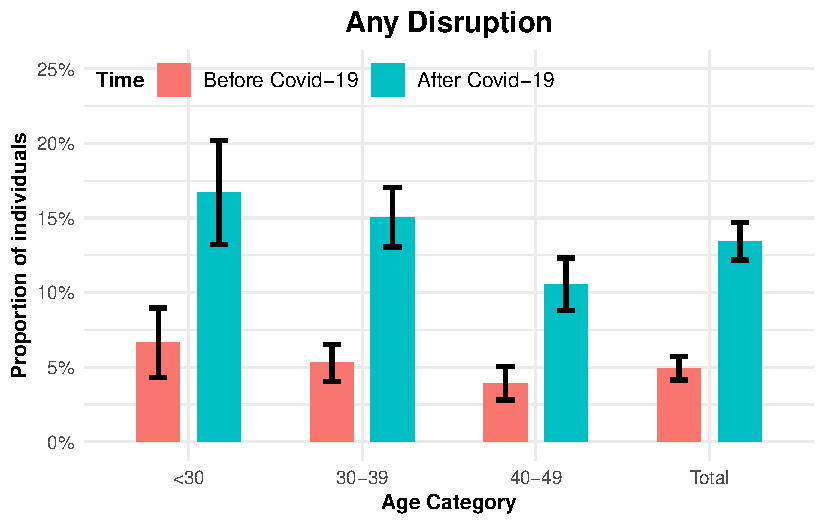
\includegraphics[keepaspectratio]{Rakai_revision_files/figure-pdf/unnamed-chunk-99-1.pdf}}

\subsubsection{Any Disruption By
Mobility}\label{any-disruption-by-mobility}

\begin{Shaded}
\begin{Highlighting}[]
\NormalTok{pr4 }\OtherTok{\textless{}{-}}\NormalTok{ summary\_by\_mobility }\SpecialCharTok{\%\textgreater{}\%} 
\FunctionTok{ggplot}\NormalTok{(}\FunctionTok{aes}\NormalTok{(}\AttributeTok{x =}\NormalTok{ mobility, }\AttributeTok{y =}\NormalTok{ proportion, }\AttributeTok{fill =}\NormalTok{ time)) }\SpecialCharTok{+}
  \FunctionTok{geom\_col}\NormalTok{(}\AttributeTok{position =} \FunctionTok{position\_dodge}\NormalTok{(}\AttributeTok{width =} \FloatTok{0.7}\NormalTok{), }\AttributeTok{width =} \FloatTok{0.5}\NormalTok{) }\SpecialCharTok{+}
  \FunctionTok{geom\_errorbar}\NormalTok{(}
    \FunctionTok{aes}\NormalTok{(}\AttributeTok{ymin =}\NormalTok{ lower, }\AttributeTok{ymax =}\NormalTok{ upper),}
    \AttributeTok{position =} \FunctionTok{position\_dodge}\NormalTok{(}\AttributeTok{width =} \FloatTok{0.7}\NormalTok{),}
    \AttributeTok{width =} \FloatTok{0.2}\NormalTok{,}
    \AttributeTok{size =} \DecValTok{1}
\NormalTok{  ) }\SpecialCharTok{+}
  \FunctionTok{scale\_y\_continuous}\NormalTok{(}\AttributeTok{labels =}\NormalTok{ scales}\SpecialCharTok{::}\FunctionTok{percent\_format}\NormalTok{(}\AttributeTok{accuracy =} \DecValTok{1}\NormalTok{), }\AttributeTok{limits =} \FunctionTok{c}\NormalTok{(}\DecValTok{0}\NormalTok{, }\FloatTok{0.26}\NormalTok{)) }\SpecialCharTok{+}
  \FunctionTok{labs}\NormalTok{(}
    \AttributeTok{title =} \StringTok{"Any Disruption"}\NormalTok{,}
    \AttributeTok{x =} \StringTok{"Mobility"}\NormalTok{,}
    \AttributeTok{y =} \StringTok{"Proportion of individuals"}\NormalTok{,}
    \AttributeTok{fill =} \StringTok{"Time"}
\NormalTok{  ) }\SpecialCharTok{+}
  \FunctionTok{theme\_minimal}\NormalTok{() }\SpecialCharTok{+}
  \FunctionTok{theme}\NormalTok{(}
    \AttributeTok{plot.title =} \FunctionTok{element\_text}\NormalTok{(}\AttributeTok{hjust =} \FloatTok{0.5}\NormalTok{, }\AttributeTok{face =} \StringTok{"bold"}\NormalTok{, }\AttributeTok{size =} \DecValTok{12}\NormalTok{),}
    \AttributeTok{axis.title.x =} \FunctionTok{element\_text}\NormalTok{(}\AttributeTok{face =} \StringTok{"bold"}\NormalTok{, }\AttributeTok{size =} \DecValTok{10}\NormalTok{),}
    \AttributeTok{axis.title.y =} \FunctionTok{element\_text}\NormalTok{(}\AttributeTok{face =} \StringTok{"bold"}\NormalTok{, }\AttributeTok{size =} \DecValTok{10}\NormalTok{),}
    \AttributeTok{legend.title =} \FunctionTok{element\_text}\NormalTok{(}\AttributeTok{face =} \StringTok{"bold"}\NormalTok{, }\AttributeTok{size =} \DecValTok{10}\NormalTok{),}
    \AttributeTok{legend.text =} \FunctionTok{element\_text}\NormalTok{(}\AttributeTok{size =} \DecValTok{10}\NormalTok{),}
    \AttributeTok{legend.position =} \FunctionTok{c}\NormalTok{(}\DecValTok{0}\NormalTok{, }\DecValTok{1}\NormalTok{), }
    \AttributeTok{legend.justification =} \FunctionTok{c}\NormalTok{(}\DecValTok{0}\NormalTok{, }\DecValTok{1}\NormalTok{),}
    \AttributeTok{legend.direction =} \StringTok{"horizontal"}
\NormalTok{  )}

\NormalTok{pr4}
\end{Highlighting}
\end{Shaded}

\pandocbounded{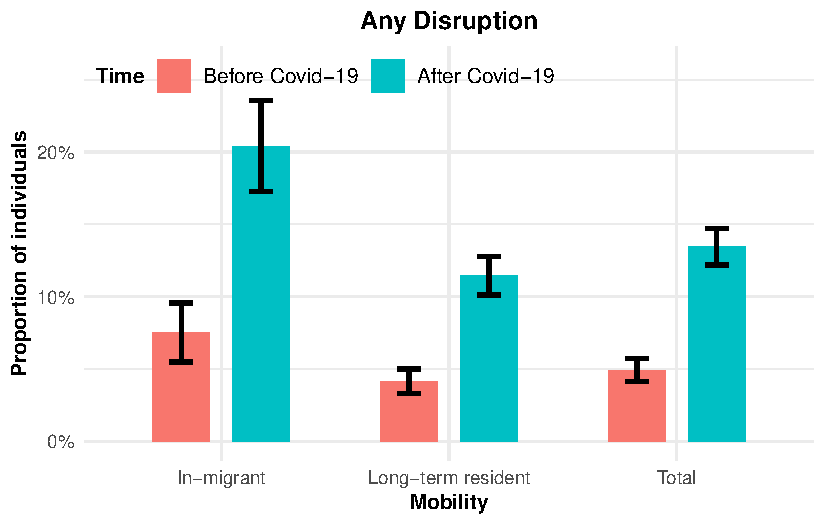
\includegraphics[keepaspectratio]{Rakai_revision_files/figure-pdf/unnamed-chunk-100-1.pdf}}

\subsubsection{Any Disruption by ART
duration}\label{any-disruption-by-art-duration}

\begin{Shaded}
\begin{Highlighting}[]
\NormalTok{pr5 }\OtherTok{\textless{}{-}}\NormalTok{ summary\_by\_art\_duration }\SpecialCharTok{\%\textgreater{}\%} 
\FunctionTok{ggplot}\NormalTok{(}\FunctionTok{aes}\NormalTok{(}\AttributeTok{x =}\NormalTok{ art\_duration, }\AttributeTok{y =}\NormalTok{ proportion, }\AttributeTok{fill =}\NormalTok{ time)) }\SpecialCharTok{+}
  \FunctionTok{geom\_col}\NormalTok{(}\AttributeTok{position =} \FunctionTok{position\_dodge}\NormalTok{(}\AttributeTok{width =} \FloatTok{0.7}\NormalTok{), }\AttributeTok{width =} \FloatTok{0.5}\NormalTok{) }\SpecialCharTok{+}
  \FunctionTok{geom\_errorbar}\NormalTok{(}
    \FunctionTok{aes}\NormalTok{(}\AttributeTok{ymin =}\NormalTok{ lower, }\AttributeTok{ymax =}\NormalTok{ upper),}
    \AttributeTok{position =} \FunctionTok{position\_dodge}\NormalTok{(}\AttributeTok{width =} \FloatTok{0.7}\NormalTok{),}
    \AttributeTok{width =} \FloatTok{0.2}\NormalTok{,}
    \AttributeTok{size =} \DecValTok{1}
\NormalTok{  ) }\SpecialCharTok{+}
  \FunctionTok{scale\_y\_continuous}\NormalTok{(}\AttributeTok{labels =}\NormalTok{ scales}\SpecialCharTok{::}\FunctionTok{percent\_format}\NormalTok{(}\AttributeTok{accuracy =} \DecValTok{1}\NormalTok{), }\AttributeTok{limits =} \FunctionTok{c}\NormalTok{(}\DecValTok{0}\NormalTok{, }\FloatTok{0.25}\NormalTok{)) }\SpecialCharTok{+}
  \FunctionTok{labs}\NormalTok{(}
    \AttributeTok{title =} \StringTok{"Any Disruption"}\NormalTok{,}
    \AttributeTok{x =} \StringTok{"ART Duration"}\NormalTok{,}
    \AttributeTok{y =} \StringTok{"Proportion of individuals"}\NormalTok{,}
    \AttributeTok{fill =} \StringTok{"Time"}
\NormalTok{  ) }\SpecialCharTok{+}
  \FunctionTok{theme\_minimal}\NormalTok{() }\SpecialCharTok{+}
  \FunctionTok{theme}\NormalTok{(}
    \AttributeTok{plot.title =} \FunctionTok{element\_text}\NormalTok{(}\AttributeTok{hjust =} \FloatTok{0.5}\NormalTok{, }\AttributeTok{face =} \StringTok{"bold"}\NormalTok{, }\AttributeTok{size =} \DecValTok{12}\NormalTok{),}
    \AttributeTok{axis.title.x =} \FunctionTok{element\_text}\NormalTok{(}\AttributeTok{face =} \StringTok{"bold"}\NormalTok{, }\AttributeTok{size =} \DecValTok{10}\NormalTok{),}
    \AttributeTok{axis.title.y =} \FunctionTok{element\_text}\NormalTok{(}\AttributeTok{face =} \StringTok{"bold"}\NormalTok{, }\AttributeTok{size =} \DecValTok{10}\NormalTok{),}
    \AttributeTok{legend.title =} \FunctionTok{element\_text}\NormalTok{(}\AttributeTok{face =} \StringTok{"bold"}\NormalTok{, }\AttributeTok{size =} \DecValTok{10}\NormalTok{),}
    \AttributeTok{legend.text =} \FunctionTok{element\_text}\NormalTok{(}\AttributeTok{size =} \DecValTok{10}\NormalTok{),}
    \AttributeTok{legend.position =} \FunctionTok{c}\NormalTok{(}\DecValTok{0}\NormalTok{, }\DecValTok{1}\NormalTok{), }
    \AttributeTok{legend.justification =} \FunctionTok{c}\NormalTok{(}\DecValTok{0}\NormalTok{, }\DecValTok{1}\NormalTok{),}
    \AttributeTok{legend.direction =} \StringTok{"horizontal"}
\NormalTok{  )}

\NormalTok{pr5}
\end{Highlighting}
\end{Shaded}

\pandocbounded{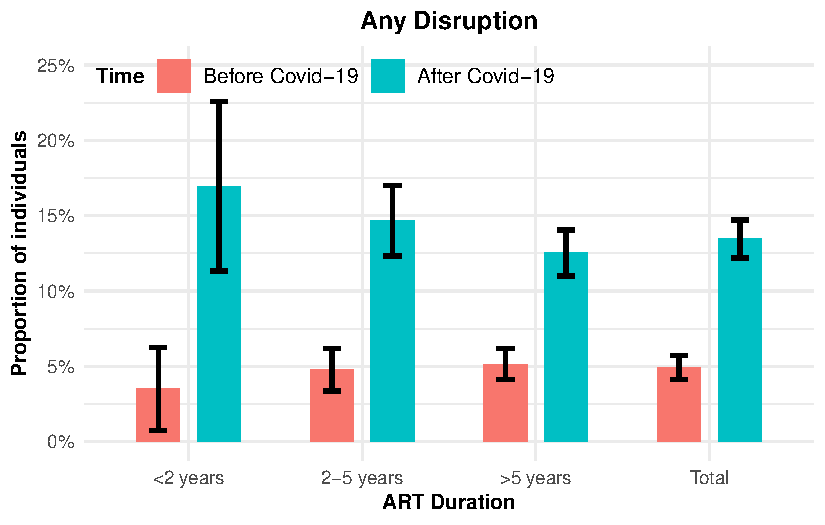
\includegraphics[keepaspectratio]{Rakai_revision_files/figure-pdf/unnamed-chunk-101-1.pdf}}

\subsubsection{Combined Plots}\label{combined-plots-1}

\paragraph{Age category}\label{age-category}

\begin{Shaded}
\begin{Highlighting}[]
\DocumentationTok{\#\#\# Combined plot}
\NormalTok{(pa1 }\SpecialCharTok{+}\NormalTok{ pa2)}\SpecialCharTok{/}\NormalTok{(pa3 }\SpecialCharTok{+}\NormalTok{ pr3)}
\end{Highlighting}
\end{Shaded}

\pandocbounded{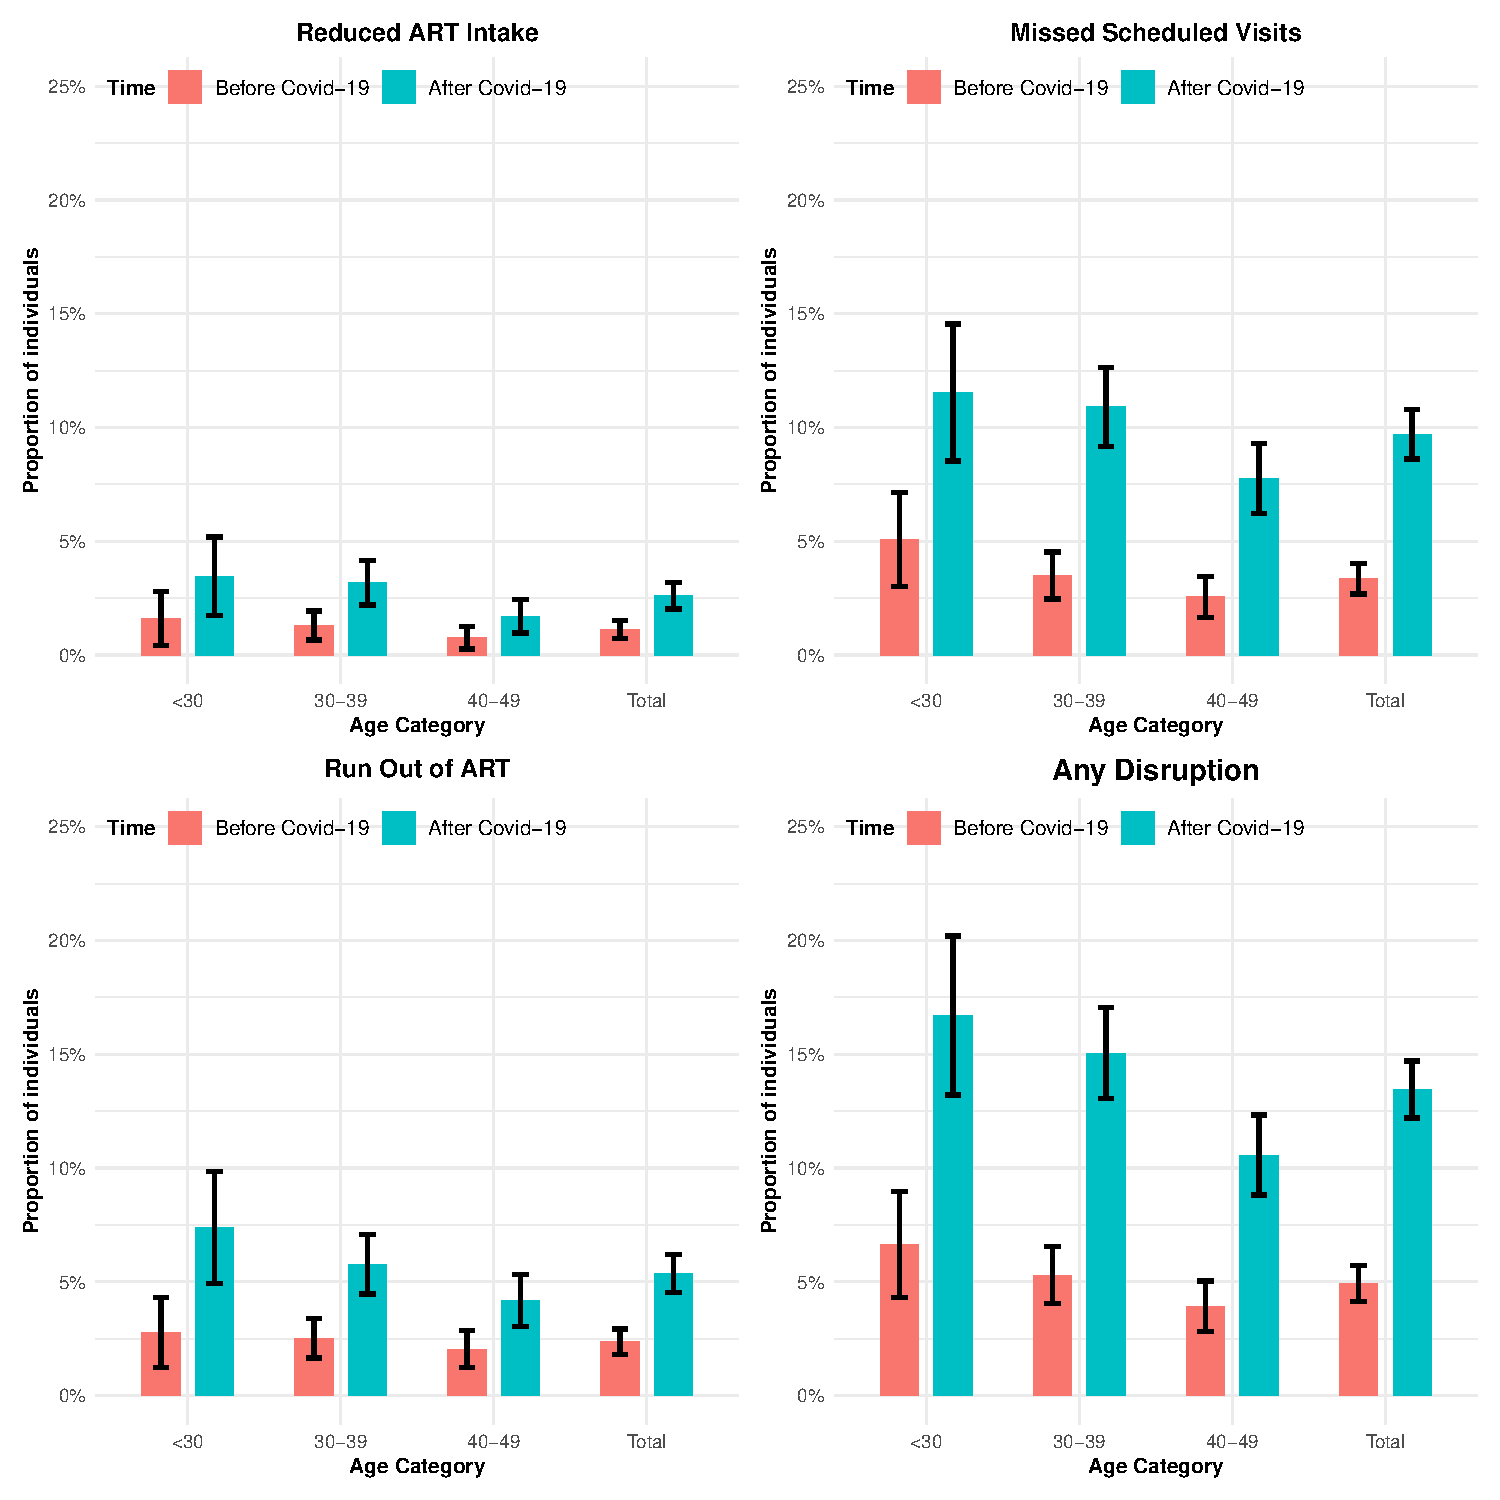
\includegraphics[keepaspectratio]{Rakai_revision_files/figure-pdf/unnamed-chunk-102-1.pdf}}

\subsubsection{Community type}\label{community-type-1}

\begin{Shaded}
\begin{Highlighting}[]
\DocumentationTok{\#\#\# Combined plot}
\NormalTok{(pc1 }\SpecialCharTok{+}\NormalTok{ pc2)}\SpecialCharTok{/}\NormalTok{(pc2 }\SpecialCharTok{+}\NormalTok{ pr2)}
\end{Highlighting}
\end{Shaded}

\pandocbounded{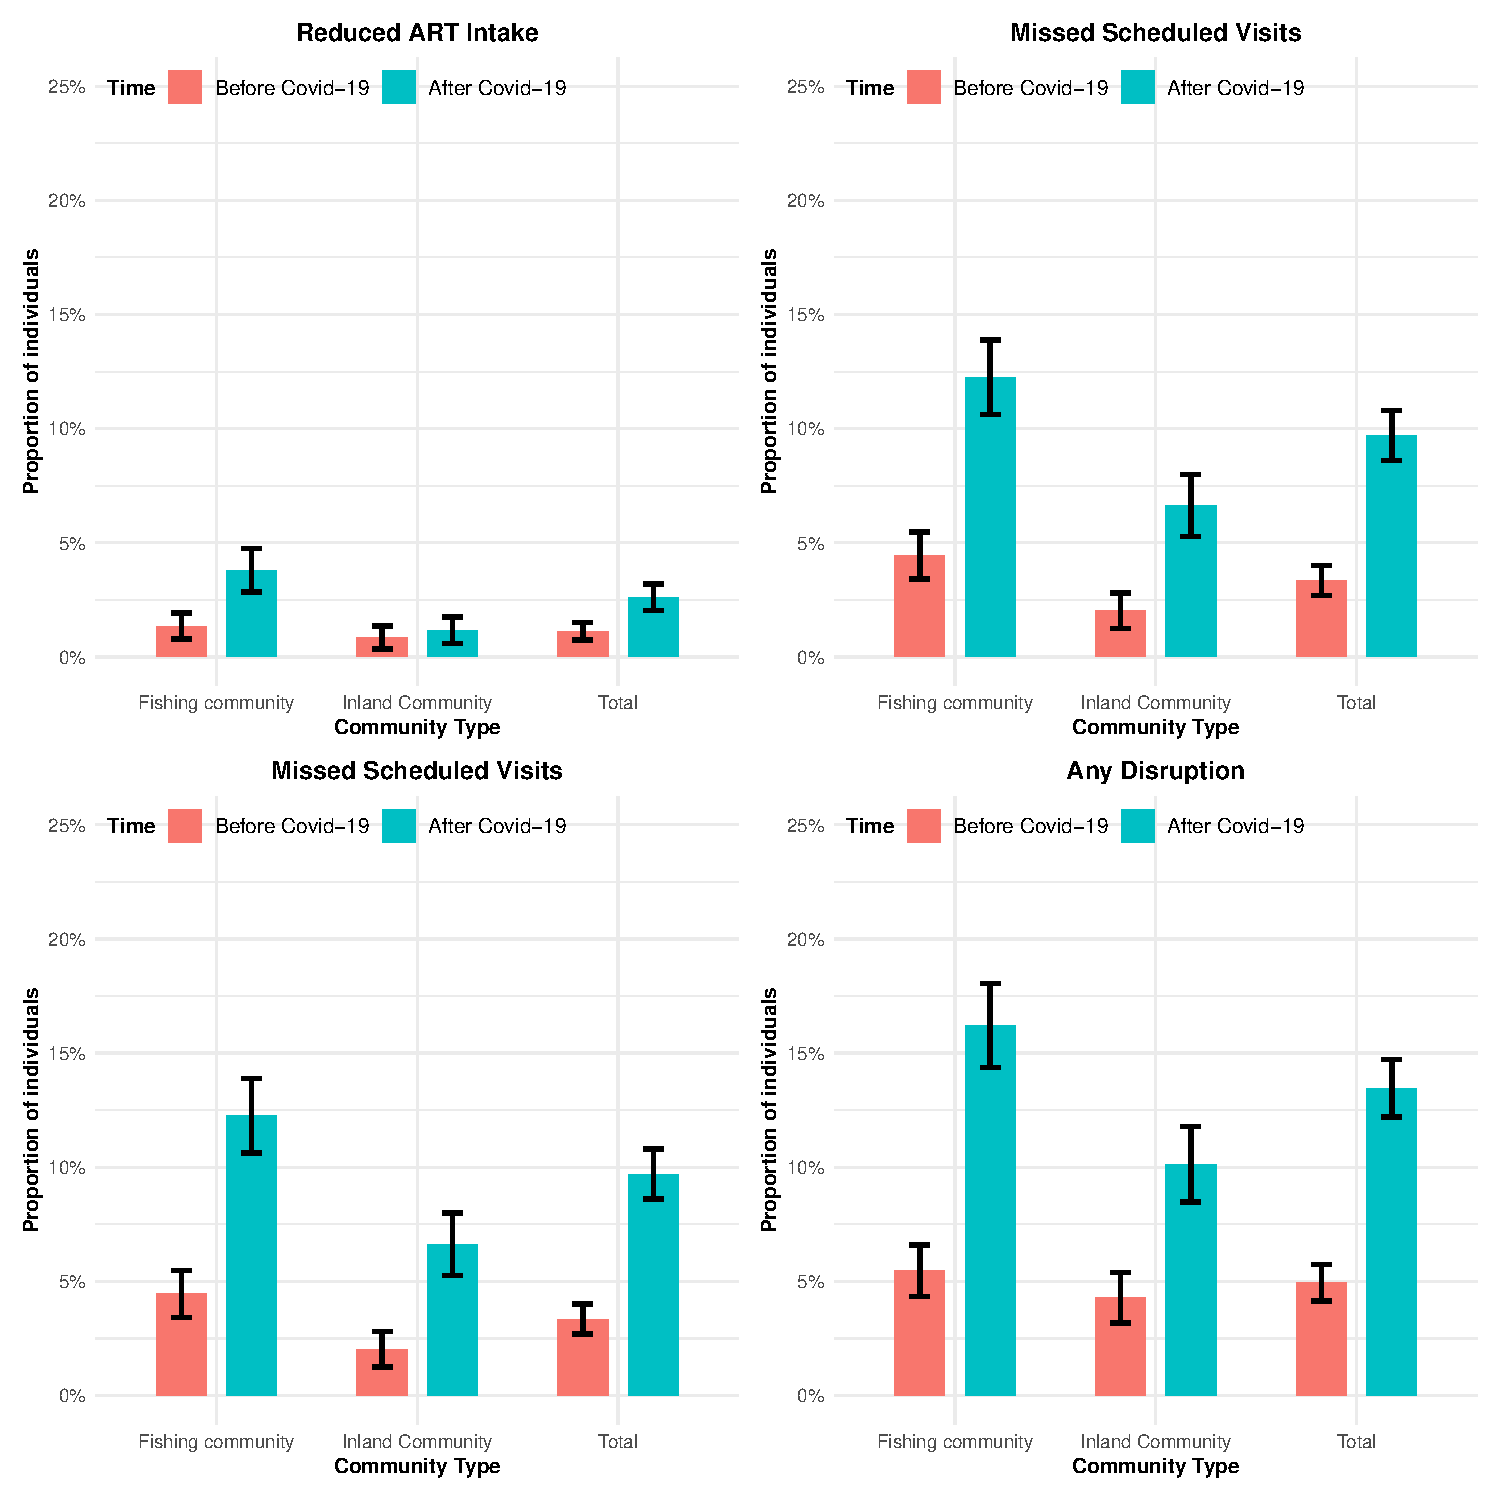
\includegraphics[keepaspectratio]{Rakai_revision_files/figure-pdf/unnamed-chunk-103-1.pdf}}

\subsubsection{Mobility}\label{mobility-1}

\begin{Shaded}
\begin{Highlighting}[]
\DocumentationTok{\#\#\# Combined plot}
\NormalTok{(pm1 }\SpecialCharTok{+}\NormalTok{ pm2)}\SpecialCharTok{/}\NormalTok{(pm3 }\SpecialCharTok{+}\NormalTok{pr4)}
\end{Highlighting}
\end{Shaded}

\pandocbounded{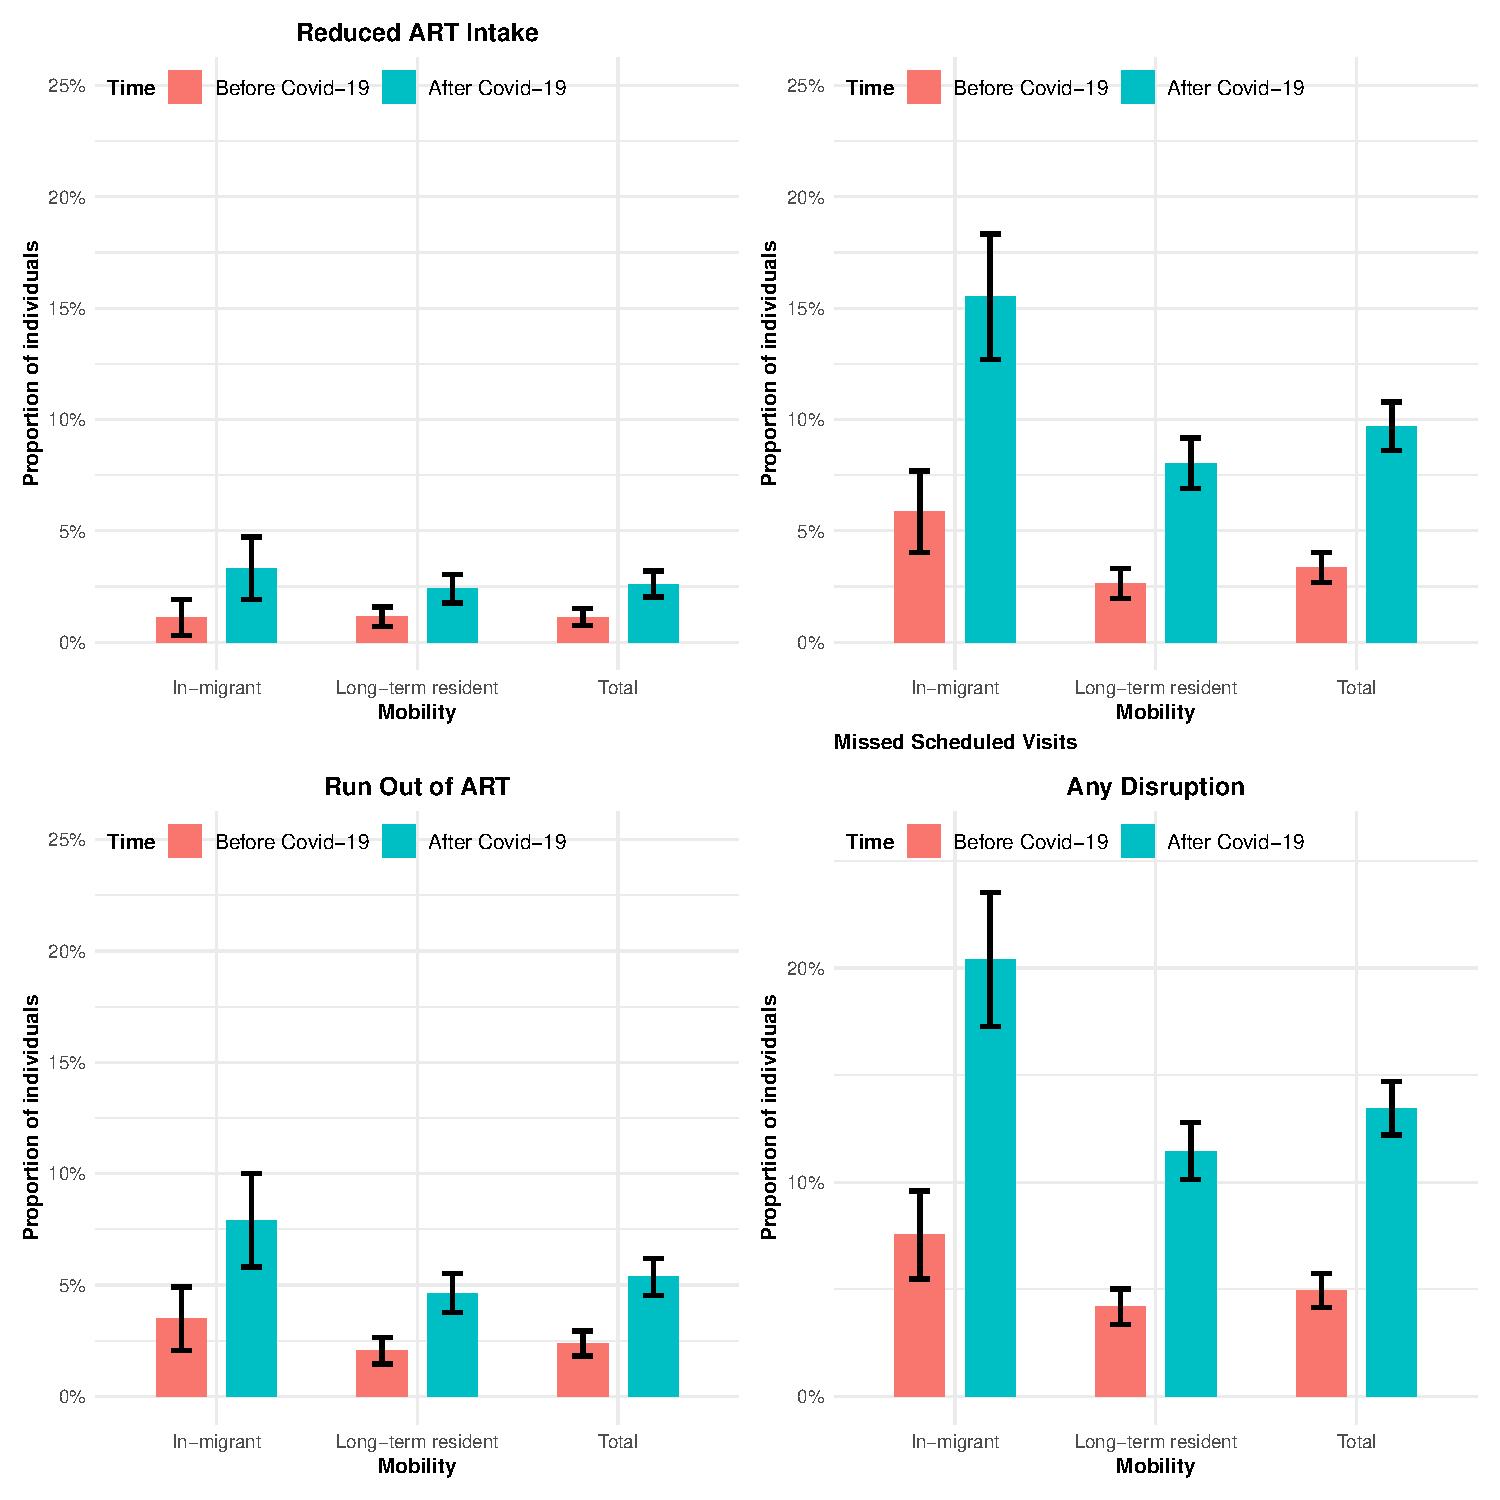
\includegraphics[keepaspectratio]{Rakai_revision_files/figure-pdf/unnamed-chunk-104-1.pdf}}

\subsubsection{ART Duration}\label{art-duration-1}

\begin{Shaded}
\begin{Highlighting}[]
\DocumentationTok{\#\#\# Combined plot}
\NormalTok{(pd1 }\SpecialCharTok{+}\NormalTok{ pd2)}\SpecialCharTok{/}\NormalTok{(pd3 }\SpecialCharTok{+}\NormalTok{ pr5)}
\end{Highlighting}
\end{Shaded}

\pandocbounded{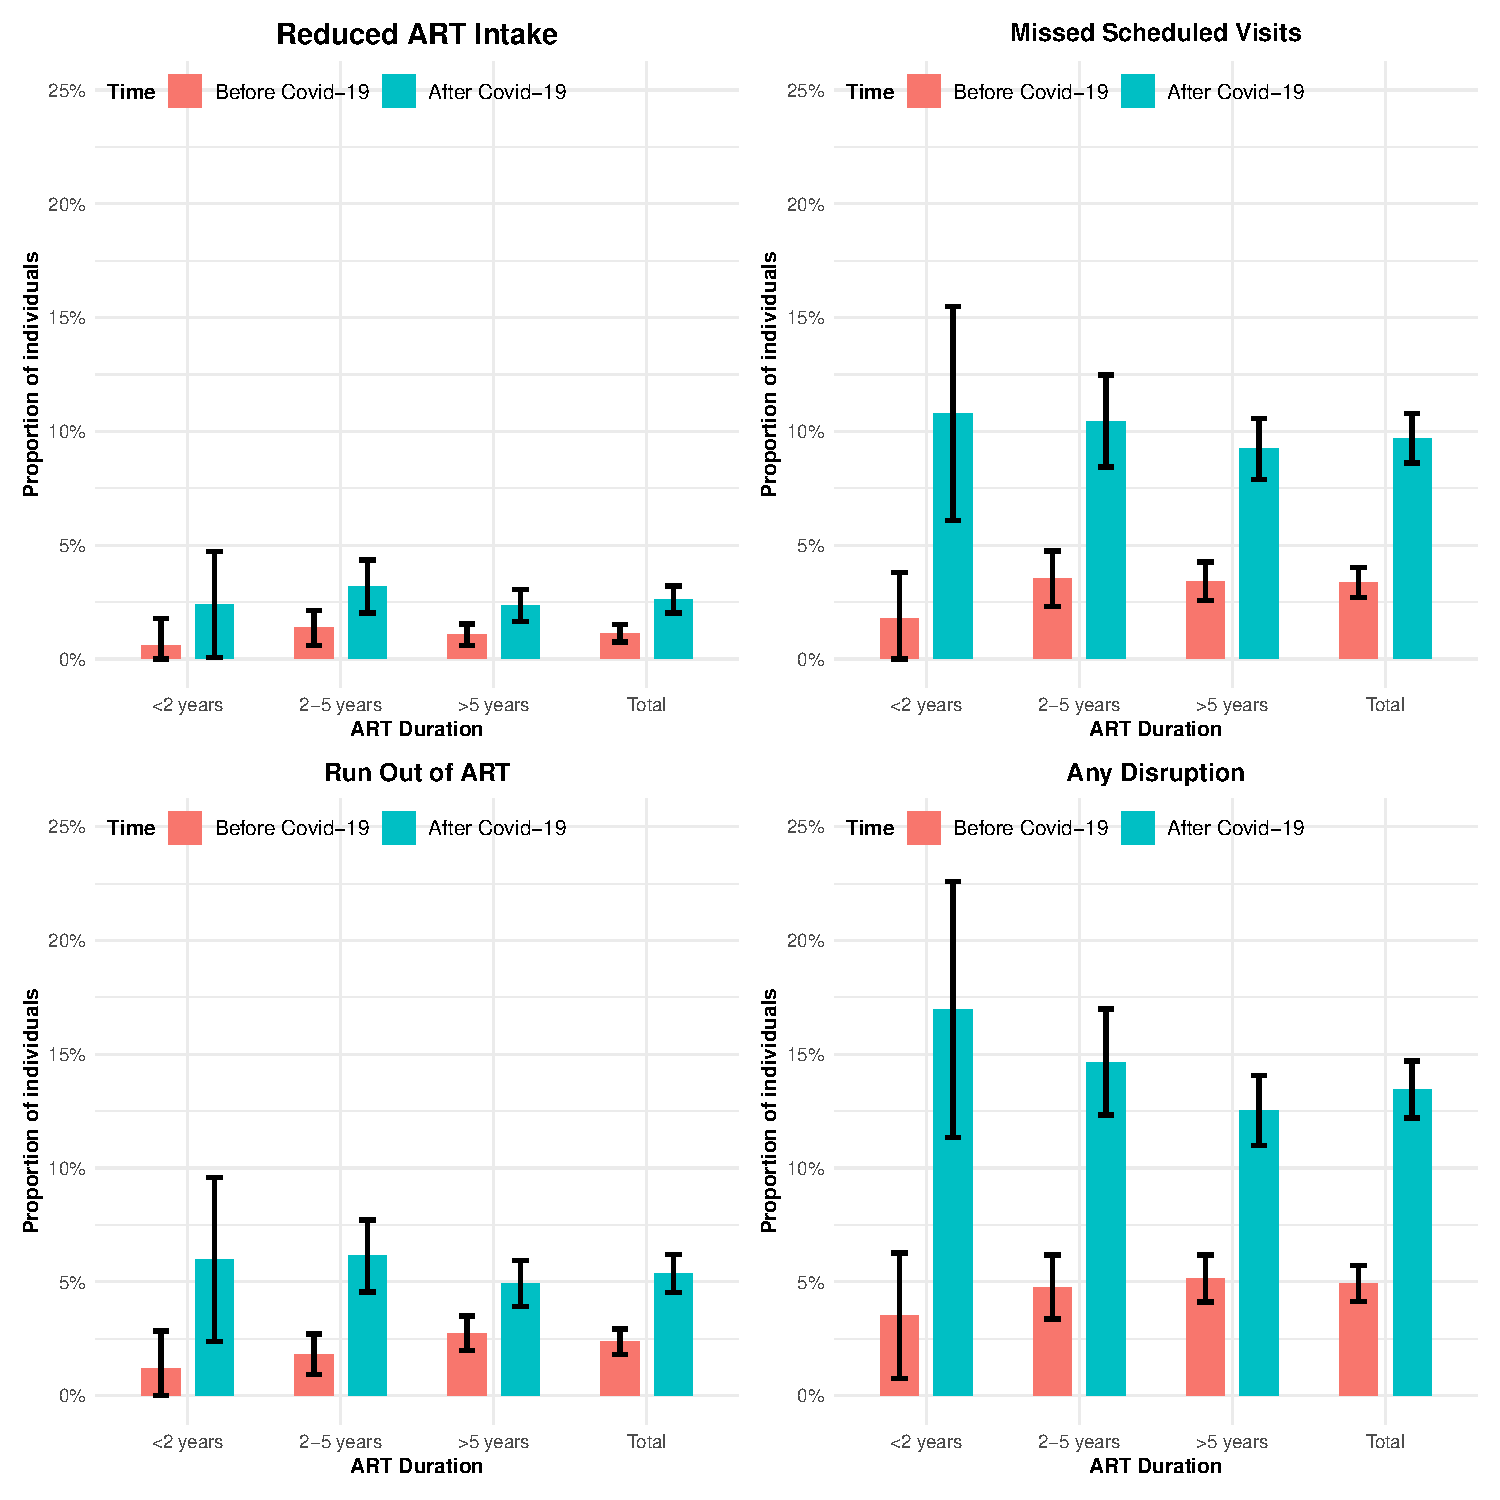
\includegraphics[keepaspectratio]{Rakai_revision_files/figure-pdf/unnamed-chunk-105-1.pdf}}

\subsubsection{Sex}\label{sex}

\begin{Shaded}
\begin{Highlighting}[]
\DocumentationTok{\#\#\# Combined plot}
\NormalTok{(ps1 }\SpecialCharTok{+}\NormalTok{ ps2)}\SpecialCharTok{/}\NormalTok{(ps3 }\SpecialCharTok{+}\NormalTok{ pr1)}
\end{Highlighting}
\end{Shaded}

\pandocbounded{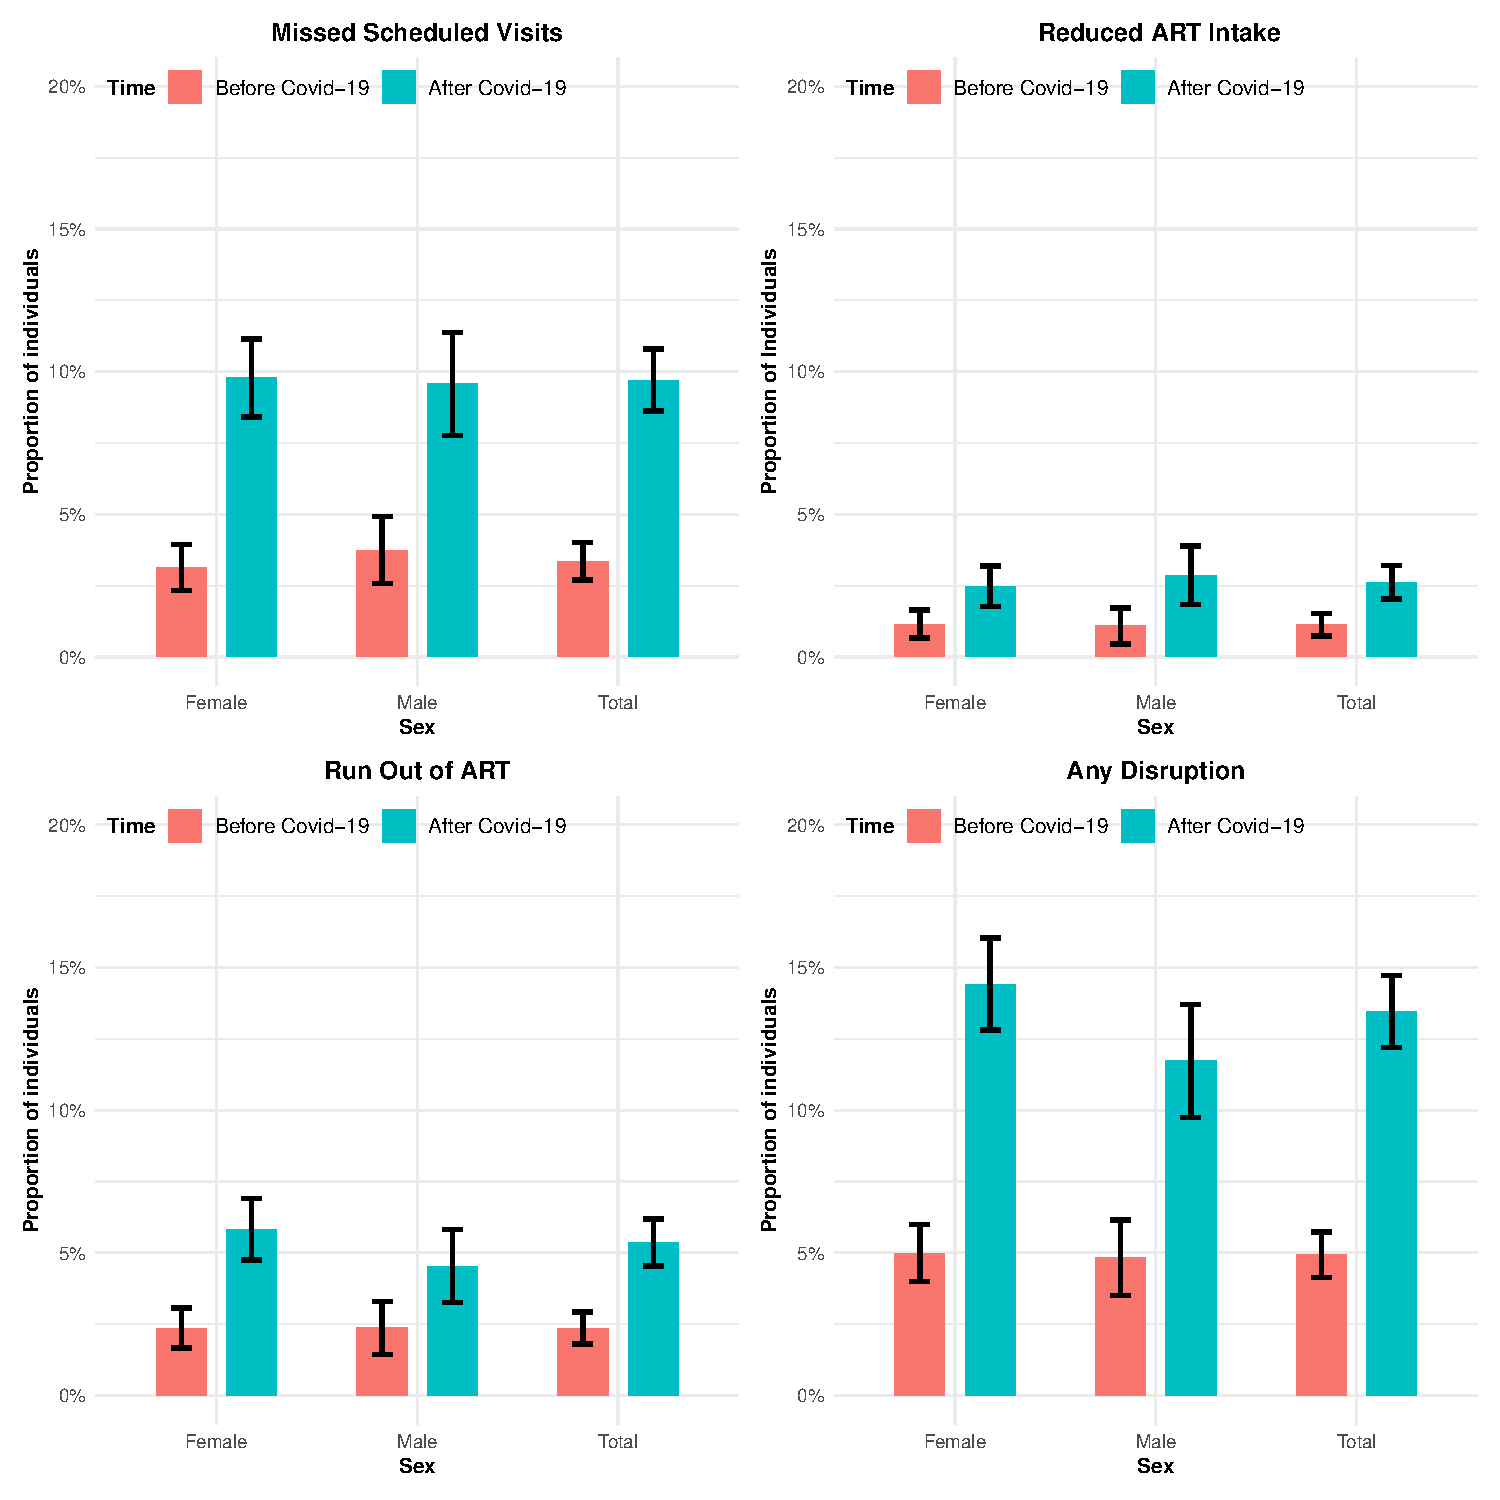
\includegraphics[keepaspectratio]{Rakai_revision_files/figure-pdf/unnamed-chunk-106-1.pdf}}




\end{document}
